% Options for packages loaded elsewhere
\PassOptionsToPackage{unicode}{hyperref}
\PassOptionsToPackage{hyphens}{url}
%
\documentclass[
  letterpaper,
  DIV=11,
  numbers=noendperiod]{scrreport}

\usepackage{amsmath,amssymb}
\usepackage{iftex}
\ifPDFTeX
  \usepackage[T1]{fontenc}
  \usepackage[utf8]{inputenc}
  \usepackage{textcomp} % provide euro and other symbols
\else % if luatex or xetex
  \usepackage{unicode-math}
  \defaultfontfeatures{Scale=MatchLowercase}
  \defaultfontfeatures[\rmfamily]{Ligatures=TeX,Scale=1}
\fi
\usepackage{lmodern}
\ifPDFTeX\else  
    % xetex/luatex font selection
  \setmonofont[Scale=0.8]{PT Mono}
\fi
% Use upquote if available, for straight quotes in verbatim environments
\IfFileExists{upquote.sty}{\usepackage{upquote}}{}
\IfFileExists{microtype.sty}{% use microtype if available
  \usepackage[]{microtype}
  \UseMicrotypeSet[protrusion]{basicmath} % disable protrusion for tt fonts
}{}
\makeatletter
\@ifundefined{KOMAClassName}{% if non-KOMA class
  \IfFileExists{parskip.sty}{%
    \usepackage{parskip}
  }{% else
    \setlength{\parindent}{0pt}
    \setlength{\parskip}{6pt plus 2pt minus 1pt}}
}{% if KOMA class
  \KOMAoptions{parskip=half}}
\makeatother
\usepackage{xcolor}
\setlength{\emergencystretch}{3em} % prevent overfull lines
\setcounter{secnumdepth}{2}
% Make \paragraph and \subparagraph free-standing
\ifx\paragraph\undefined\else
  \let\oldparagraph\paragraph
  \renewcommand{\paragraph}[1]{\oldparagraph{#1}\mbox{}}
\fi
\ifx\subparagraph\undefined\else
  \let\oldsubparagraph\subparagraph
  \renewcommand{\subparagraph}[1]{\oldsubparagraph{#1}\mbox{}}
\fi

\usepackage{color}
\usepackage{fancyvrb}
\newcommand{\VerbBar}{|}
\newcommand{\VERB}{\Verb[commandchars=\\\{\}]}
\DefineVerbatimEnvironment{Highlighting}{Verbatim}{commandchars=\\\{\}}
% Add ',fontsize=\small' for more characters per line
\usepackage{framed}
\definecolor{shadecolor}{RGB}{255,255,255}
\newenvironment{Shaded}{\begin{snugshade}}{\end{snugshade}}
\newcommand{\AlertTok}[1]{\textcolor[rgb]{0.00,0.00,0.00}{#1}}
\newcommand{\AnnotationTok}[1]{\textcolor[rgb]{0.00,0.00,0.00}{\textit{#1}}}
\newcommand{\AttributeTok}[1]{\textcolor[rgb]{0.00,0.00,0.00}{#1}}
\newcommand{\BaseNTok}[1]{\textcolor[rgb]{0.00,0.00,0.00}{#1}}
\newcommand{\BuiltInTok}[1]{\textcolor[rgb]{0.00,0.00,0.00}{#1}}
\newcommand{\CharTok}[1]{\textcolor[rgb]{0.00,0.00,0.00}{#1}}
\newcommand{\CommentTok}[1]{\textcolor[rgb]{0.00,0.00,0.00}{\textit{#1}}}
\newcommand{\CommentVarTok}[1]{\textcolor[rgb]{0.00,0.00,0.00}{\textit{#1}}}
\newcommand{\ConstantTok}[1]{\textcolor[rgb]{0.00,0.00,0.00}{#1}}
\newcommand{\ControlFlowTok}[1]{\textcolor[rgb]{0.00,0.00,0.00}{#1}}
\newcommand{\DataTypeTok}[1]{\textcolor[rgb]{0.00,0.00,0.00}{#1}}
\newcommand{\DecValTok}[1]{\textcolor[rgb]{0.00,0.00,0.00}{#1}}
\newcommand{\DocumentationTok}[1]{\textcolor[rgb]{0.00,0.00,0.00}{\textit{#1}}}
\newcommand{\ErrorTok}[1]{\textcolor[rgb]{0.00,0.00,0.00}{#1}}
\newcommand{\ExtensionTok}[1]{\textcolor[rgb]{0.00,0.00,0.00}{#1}}
\newcommand{\FloatTok}[1]{\textcolor[rgb]{0.00,0.00,0.00}{#1}}
\newcommand{\FunctionTok}[1]{\textcolor[rgb]{0.00,0.00,0.00}{#1}}
\newcommand{\ImportTok}[1]{\textcolor[rgb]{0.00,0.00,0.00}{#1}}
\newcommand{\InformationTok}[1]{\textcolor[rgb]{0.00,0.00,0.00}{\textit{#1}}}
\newcommand{\KeywordTok}[1]{\textcolor[rgb]{0.00,0.00,0.00}{#1}}
\newcommand{\NormalTok}[1]{\textcolor[rgb]{0.00,0.00,0.00}{#1}}
\newcommand{\OperatorTok}[1]{\textcolor[rgb]{0.00,0.00,0.00}{#1}}
\newcommand{\OtherTok}[1]{\textcolor[rgb]{0.00,0.00,0.00}{#1}}
\newcommand{\PreprocessorTok}[1]{\textcolor[rgb]{0.00,0.00,0.00}{#1}}
\newcommand{\RegionMarkerTok}[1]{\textcolor[rgb]{0.00,0.00,0.00}{#1}}
\newcommand{\SpecialCharTok}[1]{\textcolor[rgb]{0.00,0.00,0.00}{#1}}
\newcommand{\SpecialStringTok}[1]{\textcolor[rgb]{0.00,0.00,0.00}{#1}}
\newcommand{\StringTok}[1]{\textcolor[rgb]{0.00,0.00,0.00}{#1}}
\newcommand{\VariableTok}[1]{\textcolor[rgb]{0.00,0.00,0.00}{#1}}
\newcommand{\VerbatimStringTok}[1]{\textcolor[rgb]{0.00,0.00,0.00}{#1}}
\newcommand{\WarningTok}[1]{\textcolor[rgb]{0.00,0.00,0.00}{\textit{#1}}}

\providecommand{\tightlist}{%
  \setlength{\itemsep}{0pt}\setlength{\parskip}{0pt}}\usepackage{longtable,booktabs,array}
\usepackage{calc} % for calculating minipage widths
% Correct order of tables after \paragraph or \subparagraph
\usepackage{etoolbox}
\makeatletter
\patchcmd\longtable{\par}{\if@noskipsec\mbox{}\fi\par}{}{}
\makeatother
% Allow footnotes in longtable head/foot
\IfFileExists{footnotehyper.sty}{\usepackage{footnotehyper}}{\usepackage{footnote}}
\makesavenoteenv{longtable}
\usepackage{graphicx}
\makeatletter
\def\maxwidth{\ifdim\Gin@nat@width>\linewidth\linewidth\else\Gin@nat@width\fi}
\def\maxheight{\ifdim\Gin@nat@height>\textheight\textheight\else\Gin@nat@height\fi}
\makeatother
% Scale images if necessary, so that they will not overflow the page
% margins by default, and it is still possible to overwrite the defaults
% using explicit options in \includegraphics[width, height, ...]{}
\setkeys{Gin}{width=\maxwidth,height=\maxheight,keepaspectratio}
% Set default figure placement to htbp
\makeatletter
\def\fps@figure{htbp}
\makeatother
\newlength{\cslhangindent}
\setlength{\cslhangindent}{1.5em}
\newlength{\csllabelwidth}
\setlength{\csllabelwidth}{3em}
\newlength{\cslentryspacingunit} % times entry-spacing
\setlength{\cslentryspacingunit}{\parskip}
\newenvironment{CSLReferences}[2] % #1 hanging-ident, #2 entry spacing
 {% don't indent paragraphs
  \setlength{\parindent}{0pt}
  % turn on hanging indent if param 1 is 1
  \ifodd #1
  \let\oldpar\par
  \def\par{\hangindent=\cslhangindent\oldpar}
  \fi
  % set entry spacing
  \setlength{\parskip}{#2\cslentryspacingunit}
 }%
 {}
\usepackage{calc}
\newcommand{\CSLBlock}[1]{#1\hfill\break}
\newcommand{\CSLLeftMargin}[1]{\parbox[t]{\csllabelwidth}{#1}}
\newcommand{\CSLRightInline}[1]{\parbox[t]{\linewidth - \csllabelwidth}{#1}\break}
\newcommand{\CSLIndent}[1]{\hspace{\cslhangindent}#1}

\usepackage{booktabs}
\usepackage{longtable}

% create index
\usepackage{makeidx}
\makeindex

% Wrap 
\usepackage{listings}
\lstset{
basicstyle=\small\ttfamily,
columns=flexible,
breaklines=true
}

% wrap code blocks
\usepackage{fvextra}
    \DefineVerbatimEnvironment{Highlighting}{Verbatim}{breaklines,commandchars=\\\{\}}

% typography
\usepackage{microtype}

% https://github.com/hadley/r-pkgs/blob/main/latex/preamble.tex 
% No widow lines
\widowpenalty10000 % avoid leaving lines behind
\clubpenalty10000  % avoid creating orphans
\usepackage{booktabs}
\usepackage{longtable}
\usepackage{array}
\usepackage{multirow}
\usepackage{wrapfig}
\usepackage{float}
\usepackage{colortbl}
\usepackage{pdflscape}
\usepackage{tabu}
\usepackage{threeparttable}
\usepackage{threeparttablex}
\usepackage[normalem]{ulem}
\usepackage{makecell}
\usepackage{xcolor}
\KOMAoption{captions}{tableheading}
\makeatletter
\@ifpackageloaded{tcolorbox}{}{\usepackage[skins,breakable]{tcolorbox}}
\@ifpackageloaded{fontawesome5}{}{\usepackage{fontawesome5}}
\definecolor{quarto-callout-color}{HTML}{909090}
\definecolor{quarto-callout-note-color}{HTML}{0758E5}
\definecolor{quarto-callout-important-color}{HTML}{CC1914}
\definecolor{quarto-callout-warning-color}{HTML}{EB9113}
\definecolor{quarto-callout-tip-color}{HTML}{00A047}
\definecolor{quarto-callout-caution-color}{HTML}{FC5300}
\definecolor{quarto-callout-color-frame}{HTML}{acacac}
\definecolor{quarto-callout-note-color-frame}{HTML}{4582ec}
\definecolor{quarto-callout-important-color-frame}{HTML}{d9534f}
\definecolor{quarto-callout-warning-color-frame}{HTML}{f0ad4e}
\definecolor{quarto-callout-tip-color-frame}{HTML}{02b875}
\definecolor{quarto-callout-caution-color-frame}{HTML}{fd7e14}
\makeatother
\makeatletter
\makeatother
\makeatletter
\@ifpackageloaded{bookmark}{}{\usepackage{bookmark}}
\makeatother
\makeatletter
\@ifpackageloaded{caption}{}{\usepackage{caption}}
\AtBeginDocument{%
\ifdefined\contentsname
  \renewcommand*\contentsname{Table of contents}
\else
  \newcommand\contentsname{Table of contents}
\fi
\ifdefined\listfigurename
  \renewcommand*\listfigurename{List of Figures}
\else
  \newcommand\listfigurename{List of Figures}
\fi
\ifdefined\listtablename
  \renewcommand*\listtablename{List of Tables}
\else
  \newcommand\listtablename{List of Tables}
\fi
\ifdefined\figurename
  \renewcommand*\figurename{Figure}
\else
  \newcommand\figurename{Figure}
\fi
\ifdefined\tablename
  \renewcommand*\tablename{Table}
\else
  \newcommand\tablename{Table}
\fi
}
\@ifpackageloaded{float}{}{\usepackage{float}}
\floatstyle{ruled}
\@ifundefined{c@chapter}{\newfloat{codelisting}{h}{lop}}{\newfloat{codelisting}{h}{lop}[chapter]}
\floatname{codelisting}{File}
\newcommand*\listoflistings{\listof{codelisting}{List of Listings}}
\usepackage{amsthm}
\theoremstyle{definition}
\newtheorem{example}{Example}[chapter]
\theoremstyle{remark}
\AtBeginDocument{\renewcommand*{\proofname}{Proof}}
\newtheorem*{remark}{Remark}
\newtheorem*{solution}{Solution}
\makeatother
\makeatletter
\@ifpackageloaded{caption}{}{\usepackage{caption}}
\@ifpackageloaded{subcaption}{}{\usepackage{subcaption}}
\makeatother
\makeatletter
\@ifpackageloaded{tcolorbox}{}{\usepackage[skins,breakable]{tcolorbox}}
\makeatother
\makeatletter
\@ifundefined{shadecolor}{\definecolor{shadecolor}{rgb}{.97, .97, .97}}
\makeatother
\makeatletter
\@ifundefined{codebgcolor}{\definecolor{codebgcolor}{HTML}{f9f9f9}}
\makeatother
\makeatletter
\makeatother
\makeatletter
\@ifpackageloaded{fontawesome5}{}{\usepackage{fontawesome5}}
\makeatother
\ifLuaTeX
  \usepackage{selnolig}  % disable illegal ligatures
\fi
\IfFileExists{bookmark.sty}{\usepackage{bookmark}}{\usepackage{hyperref}}
\IfFileExists{xurl.sty}{\usepackage{xurl}}{} % add URL line breaks if available
\urlstyle{same} % disable monospaced font for URLs
% Make links footnotes instead of hotlinks:
\DeclareRobustCommand{\href}[2]{#2\footnote{\url{#1}}}
\hypersetup{
  pdftitle={Quantitative Text Analysis for Linguistics},
  pdfauthor={Jerid Francom},
  hidelinks,
  pdfcreator={LaTeX via pandoc}}

\title{Quantitative Text Analysis for Linguistics}
\usepackage{etoolbox}
\makeatletter
\providecommand{\subtitle}[1]{% add subtitle to \maketitle
  \apptocmd{\@title}{\par {\large #1 \par}}{}{}
}
\makeatother
\subtitle{Reproducible Research using R}
\author{Jerid Francom}
\date{August 2, 2023}

\begin{document}
\maketitle
\ifdefined\Shaded\renewenvironment{Shaded}{\begin{tcolorbox}[frame hidden, colback={codebgcolor}, breakable, boxrule=0pt, enhanced, sharp corners, borderline west={3pt}{0pt}{shadecolor}]}{\end{tcolorbox}}\fi

\renewcommand*\contentsname{Table of contents}
{
\setcounter{tocdepth}{2}
\tableofcontents
}
\bookmarksetup{startatroot}

\hypertarget{welcome}{%
\chapter*{Welcome}\label{welcome}}

\markboth{Welcome}{Welcome}

The goal of this textbook is to provide readers with foundational
knowledge and practical skills in quantitative text analysis using the R
programming language.

By the end of this textbook, readers will be able to identify, interpret
and evaluate data analysis procedures and results to support research
questions within language science. Additionally, readers will gain
experience in designing and implementing research projects that involve
processing and analyzing textual data employing modern programming
strategies. This textbook aims to instill a strong sense of reproducible
research practices, which are critical for promoting transparency,
verification, and sharing of research findings.

This textbook is geared towards advanced undergraduates, graduate
students, and researchers looking to expand their methodological
toolbox. It assumes no prior knowledge of programming or quantitative
methods and prioritizes practical application and intuitive
understanding over technical details.

\textbf{About the author}

Dr.~Jerid Francom is Associate Professor of Spanish and Linguistics at
Wake Forest University. His research focuses on the use of language
corpora from a variety of sources (news, social media, and other
internet sources) to better understand the linguistic and cultural
similarities and differences between language varieties for both
scholarly and pedagogical projects. He has published on topics including
the development, annotation, and evaluation of linguistic corpora and
analyzed corpora through corpus, psycholinguistic, and computational
methodologies. He also has experience working with and teaching
statistical programming with R.

\hypertarget{license}{%
\section*{License}\label{license}}
\addcontentsline{toc}{section}{License}

\markright{License}

This work by \href{https://francojc.github.io/}{Jerid C. Francom} is
licensed under a Creative Commons
Attribution-NonCommercial-NoDerivatives 4.0 International License.

\hypertarget{credits}{%
\section*{Credits}\label{credits}}
\addcontentsline{toc}{section}{Credits}

\markright{Credits}

\href{https://fontawesome.com/}{Font Awesome Icons} are SIL OFL 1.1
Licensed

\hypertarget{acknowledgements}{%
\section*{Acknowledgements}\label{acknowledgements}}
\addcontentsline{toc}{section}{Acknowledgements}

\markright{Acknowledgements}

The development of this book has benefited from the generous feedback
from the following people: Andrea Bowling, Caroline Brady, Declan
Golsen, Asya Little, Claudia Valdez, \emph{(add your name here!)}. As
always, any errors or omissions are my own.

\hypertarget{build-information}{%
\section*{Build information}\label{build-information}}
\addcontentsline{toc}{section}{Build information}

\markright{Build information}

This textbook was built with the \texttt{quarto} package
(\protect\hyperlink{ref-R-quarto}{Allaire 2022}) and the
\texttt{bookdown} package (\protect\hyperlink{ref-R-bookdown}{Xie
2023a}) for R. The source code for this book is available on
\href{https://github.com/qtalr/book}{GitHub}.

This version of the textbook was built with R version 4.3.1 (2023-06-16)
on macOS Ventura 13.4.1 with the following packages:

\begin{longtable}[]{@{}
  >{\raggedright\arraybackslash}p{(\columnwidth - 4\tabcolsep) * \real{0.1042}}
  >{\raggedright\arraybackslash}p{(\columnwidth - 4\tabcolsep) * \real{0.0833}}
  >{\raggedright\arraybackslash}p{(\columnwidth - 4\tabcolsep) * \real{0.8125}}@{}}
\toprule\noalign{}
\begin{minipage}[b]{\linewidth}\raggedright
package
\end{minipage} & \begin{minipage}[b]{\linewidth}\raggedright
version
\end{minipage} & \begin{minipage}[b]{\linewidth}\raggedright
source
\end{minipage} \\
\midrule\noalign{}
\endhead
\bottomrule\noalign{}
\endlastfoot
dplyr & 1.1.2 & CRAN (R 4.3.0) \\
forcats & 1.0.0 & CRAN (R 4.3.0) \\
ggplot2 & 3.4.2 & CRAN (R 4.3.0) \\
here & 1.0.1 & CRAN (R 4.3.0) \\
knitr & 1.43 & CRAN (R 4.3.0) \\
lubridate & 1.9.2 & CRAN (R 4.3.0) \\
purrr & 1.0.1 & CRAN (R 4.3.0) \\
qtalrkit & 0.0.2.0 & Github
(qtalr/qtalrkit@34a75e96a47e624b5af5f253c1d74f1659589ceb) \\
readr & 2.1.4 & CRAN (R 4.3.0) \\
readtext & 0.90 & CRAN (R 4.3.0) \\
rmarkdown & 2.23 & CRAN (R 4.3.1) \\
stringr & 1.5.0 & CRAN (R 4.3.0) \\
tadr & 0.1.2 & local
(/Users/francojc/Documents/Academic/Research/Projects/1Active/tad/tadr) \\
tibble & 3.2.1 & CRAN (R 4.3.0) \\
tidyr & 1.3.0 & CRAN (R 4.3.0) \\
tidytext & 0.4.1 & CRAN (R 4.3.0) \\
tidyverse & 2.0.0 & CRAN (R 4.3.1) \\
webshot & 0.5.5 & CRAN (R 4.3.1) \\
\end{longtable}

\bookmarksetup{startatroot}

\hypertarget{sec-preface}{%
\chapter*{Preface}\label{sec-preface}}
\addcontentsline{toc}{chapter}{Preface}

\markboth{Preface}{Preface}

\begin{tcolorbox}[enhanced jigsaw, leftrule=.75mm, title=\textcolor{quarto-callout-tip-color}{\faLightbulb}\hspace{0.5em}{Draft}, coltitle=black, opacityback=0, titlerule=0mm, arc=.35mm, bottomtitle=1mm, opacitybacktitle=0.6, colframe=quarto-callout-tip-color-frame, rightrule=.15mm, toptitle=1mm, left=2mm, colback=white, breakable, toprule=.15mm, bottomrule=.15mm, colbacktitle=quarto-callout-tip-color!10!white]

Ready for review.

\end{tcolorbox}

\begin{quote}
The journey of a thousand miles begins with one step.

--- Lao Tzu
\end{quote}

\begin{tcolorbox}[enhanced jigsaw, rightrule=.15mm, leftrule=.75mm, opacityback=0, arc=.35mm, colback=white, breakable, toprule=.15mm, bottomrule=.15mm, left=2mm]

\textbf{\faIcon{list-alt} Outcomes}

\begin{itemize}
\tightlist
\item
  Comprehend the book's rationale, learning goals, and pedagogical
  approach.
\item
  Navigate and engage with the book's structure and content effectively.
\item
  Interpret conventions used in the book reliably.
\item
  Set up the computing environment and utilize textbook and support
  resources for an optimal learning experience.
\end{itemize}

\end{tcolorbox}

The purpose of this chapter is to present the rationale behind this
textbook, outline the key learning objectives, describe the pedagogical
approach, and identify the intended audience. Additionally, this chapter
will provide readers with a guide to the book's structure and the scope
of its content, as well as instructions for the instructor and a summary
of supporting resources available. Finally, this chapter will provide
readers with information on setting up their computing environment and
where to seek support.

\hypertarget{sec-p-rationale}{%
\section*{Rationale}\label{sec-p-rationale}}
\addcontentsline{toc}{section}{Rationale}

\markright{Rationale}

Data science, an interdisciplinary field that combines knownledge and
skills from statistics, computer science, and domain-specific expertise
to extract meaningful insight from structured and unstructured data, has
emerged as an exciting and rapidly growing field in recent years, driven
in large part by the increase in computing power available to the
average individual and the abundance of electronic data now available
through the internet. These advances have become an integral part of the
modern scientific landscape, with data-driven insights now being used to
inform decision-making in a wide variety of academic fields, including
linguistics and language-related disciplines.

This textbook seeks to meet this growing demand by providing an
introduction to the fundamental concepts and practical programming
skills from data science applied to the task of quantitative text
analysis. It is intended primarily for undergraduate students, but may
also be useful for graduates and researchers seeking to expand their
methodological toolbox. The textbook takes a pedagogical approach which
assumes no prior experience with statistics or programming, making it an
accessible resource for novices beginning their exploration of
quantitative text analysis methods.

\hypertarget{sec-p-aims}{%
\section*{Aims}\label{sec-p-aims}}
\addcontentsline{toc}{section}{Aims}

\markright{Aims}

The overarching goal of this textbook is to provide readers with
foundational knowledge and practical skills to conduct and evaluate
quantitative text analysis using the R programming language and other
open source tools and technologies. The specific aims are to develop the
reader's proficiency in three main areas:

\begin{itemize}
\tightlist
\item
  \textbf{Data literacy:} Identify, interpret and evaluate data analysis
  procedures and results
\end{itemize}

\begin{quote}
Throughout this textbook we will explore topics which will help you
understand how data analysis methods derive insight from data. In this
process you will be encouraged to critically evaluate connections across
linguistic and language-related disciplines using data analysis
knowledge and skills. Data literacy is an invaluable skillset for
academics and professionals but also is an indispensable aptitude for in
the 21st century citizens to navigate and actively participate in the
`Information Age' in which we live
(\protect\hyperlink{ref-Carmi2020}{Carmi et al. 2020}).
\end{quote}

\begin{itemize}
\tightlist
\item
  \textbf{Research skills:} Design, implement, and communicate
  quantitative research
\end{itemize}

\begin{quote}
This aim does not differ significantly, in spirit, from common learning
outcomes in a research methods course. However, working with text will
incur a series of key steps in the selection, collection, and
preparation of the data that are unique to text analysis projects. In
addition, I will stress the importance of research documentation and
creating reproducible research as an integral part of modern scientific
inquiry (\protect\hyperlink{ref-Buckheit1995}{Buckheit and Donoho
1995}).
\end{quote}

\begin{itemize}
\tightlist
\item
  \textbf{Programming skills:} Apply programmatic strategies to develop
  and collaborate on reproducible research projects
\end{itemize}

\begin{quote}
Modern data analysis, and by extension, text analysis is conducted using
programming. There are various key reasons for this: a programming
approach (1) affords researchers unlimited research freedom --if you can
envision it, you can program it, (2) underlies well-documented and
reproducible research (\protect\hyperlink{ref-Gandrud2015}{Gandrud
2015}), and (3) invites researchers to engage more intimately with the
data and the methods for analysis.
\end{quote}

These aims are important for linguistics students because they provide a
foundation for concepts and in the skills required to succeed in the
rapidly evolving landscape of 21st-century research. These abilities
enable researchers to evaluate and conduct high-quality empirical
investigation across linguistic fields on a wide variety of topics.
Moreover, these skills go beyond linguistics research; they are widely
applicable across many disciplines where quantitative data analysis and
programming are becoming increasingly important. Thus, this textbook
provides students with a comprehensive introduction to quantitative text
analysis that is relevant to linguistics research and that equips them
with valuable skills for their future careers.

\hypertarget{sec-p-approach}{%
\section*{Approach}\label{sec-p-approach}}
\addcontentsline{toc}{section}{Approach}

\markright{Approach}

The approach taken in this textbook is designed to accomodate
linguistics students and researchers with little to no prior experience
with programming or quantitative methods. With this in mind the
objective is connect conceptual understanding with practical
application. Real-world data and research tasks relevant to linguistics
are used thoughtout the book to provide context and to motivate the
learning process\footnote{Research data and questions are primarily
  based on English for wide accessibility as it is the \emph{de facto}
  language of academics and research. However, the methods and
  techniques presented in this textbook are applicable to many other
  languages.}. Furthermore, as an introduction to the field, the
textbook focuses on the most common and fundamental methods and
techniques for quantitative text analysis and prioritizes breadth over
depth and intuitive understanding over technical explanations. On the
programming side, the Tidyverse approach to programming in R will be
adopted. This approach provides a consistent syntax across different
packages and is known for its legibility, making it easier for readers
to understand and write code. Together, these strategies form an
approach that is intended to provide readers with an accessible resource
to gain a foothold in the field and to equip them with the knowledge and
skills to apply quantitative text analysis in their own research.

\hypertarget{sec-p-structure}{%
\section*{Structure}\label{sec-p-structure}}
\addcontentsline{toc}{section}{Structure}

\markright{Structure}

The aims and approach described above is reflected in the overall
structure of the book and each chapter.

\hypertarget{sec-p-structure-book}{%
\subsection*{Book level}\label{sec-p-structure-book}}
\addcontentsline{toc}{subsection}{Book level}

At the book level, there are five interdependent parts:

Part I ``Orientation'' provides the necessary background knowledge to
situate quantitative text analysis in the wider context of data analysis
and linguistic research and to provide a clearer picture of what text
analysis entails and its range of applications.

The subsequent parts are directly aligned with the data analysis
process. The building blocks of this process are reflected in `Data to
Insight Hierarchy (DIKI)' visualized in
Figure~\ref{fig-diki-hierarchy}\footnote{Adapted from Ackoff
  (\protect\hyperlink{ref-Ackoff1989}{1989}) and Rowley
  (\protect\hyperlink{ref-Rowley2007}{2007}).}.

\begin{figure}[H]

{\centering 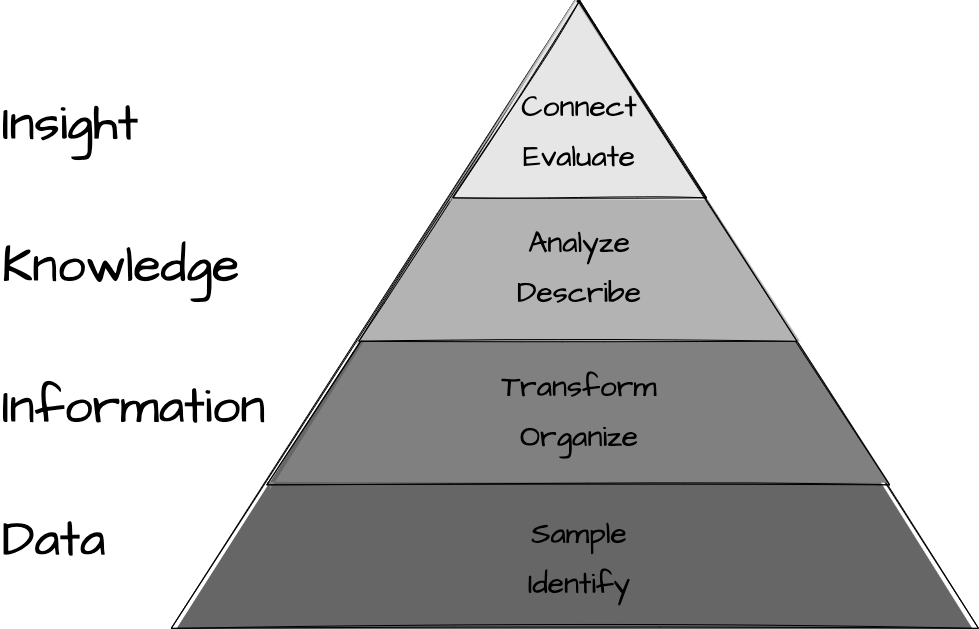
\includegraphics[width=3.26in,height=\textheight]{figures/preface/p-diki.drawio.png}

}

\caption{\label{fig-diki-hierarchy}Data to Insight Hierarchy (DIKI)}

\end{figure}

The DIKI Hierarchy highlights the stages and intermediate steps required
to derive insight from data. Part II ``Foundations'' provides a
conceptual introduction to the DIKI Hierarchy and establishes
foundational knowledge about data, information, knowledge, and insight
which is fundamental to developing a viable research plan.

Parts III ``Preparation'' and IV ``Analysis'' focus on the
implementation process. Part III covers the steps involved in preparing
data for analysis, including data acquisition, curation, and
transformation. Part IV covers the steps involved in conducting
analysis, including exploratory, predictive, and inferential data
analysis.

The final part, Part V ``Communication'', covers the final stage of the
data analysis process, which is to communicate the results of the
analysis. This includes the structure and content of research reports as
well as the process of publishing, sharing, and collaborating on
research.

\hypertarget{sec-p-structure-chapter}{%
\subsection*{Chapter level}\label{sec-p-structure-chapter}}
\addcontentsline{toc}{subsection}{Chapter level}

At the chapter level, both conceptual and programming skills are
developed in stages\footnote{These stages attempt to capture the general
  progression of learning reflected in Bloom's Taxonomy (see Krathwohl
  (\protect\hyperlink{ref-Krathwohl2002}{2002}) for a description and
  revision).}. The chapter-level structure is consistent across chapters
and can be seen in Table~\ref{tbl-structure-approach}.

\hypertarget{tbl-structure-approach}{}
\begin{longtable}[]{@{}
  >{\raggedright\arraybackslash}p{(\columnwidth - 6\tabcolsep) * \real{0.1500}}
  >{\raggedright\arraybackslash}p{(\columnwidth - 6\tabcolsep) * \real{0.5500}}
  >{\raggedright\arraybackslash}p{(\columnwidth - 6\tabcolsep) * \real{0.1500}}
  >{\raggedright\arraybackslash}p{(\columnwidth - 6\tabcolsep) * \real{0.1500}}@{}}
\caption{\label{tbl-structure-approach}The general structure of a
chapter including: the component, its purpose, where to find the
resource, and the target learning stage.}\tabularnewline
\toprule\noalign{}
\begin{minipage}[b]{\linewidth}\raggedright
Component
\end{minipage} & \begin{minipage}[b]{\linewidth}\raggedright
Purpose
\end{minipage} & \begin{minipage}[b]{\linewidth}\raggedright
Resource
\end{minipage} & \begin{minipage}[b]{\linewidth}\raggedright
Stage
\end{minipage} \\
\midrule\noalign{}
\endfirsthead
\toprule\noalign{}
\begin{minipage}[b]{\linewidth}\raggedright
Component
\end{minipage} & \begin{minipage}[b]{\linewidth}\raggedright
Purpose
\end{minipage} & \begin{minipage}[b]{\linewidth}\raggedright
Resource
\end{minipage} & \begin{minipage}[b]{\linewidth}\raggedright
Stage
\end{minipage} \\
\midrule\noalign{}
\endhead
\bottomrule\noalign{}
\endlastfoot
Outcomes & Identify the learning objectives for the chapter & Textbook &
Introduction \\
Overview & Provide a brief introduction to the chapter topic & Textbook
& Introduction \\
Coding Lessons & Teach programming techniques with hands-on interactive
exercises & GitHub & Skills \\
Content & Combine conceptual discussions and programming skills,
incorporating thought-provoking questions, relevant studies, and
advanced topic references & Textbook & Knowledge \\
Recipes & Offer step-by-step programming examples related to the chapter
& Resources website & Comprehension \\
Labs & Allow readers to apply chapter-specific concepts and techniques &
GitHub & Application \\
Summary & Review the key concepts and skills covered in the chapter &
Textbook & Review \\
Questions & Assess and expand the reader's knowledge and abilities &
Textbook & Assessment \\
\end{longtable}

Each chapter will begin with a list of key learning outcomes followed by
a brief introduction to the chapter's content. The goal is to orient the
reader to the chapter. Next there will be a prompt to complete the
interactive coding lesson(s) to introduce reader's to key programming
concepts related to the chapter though hands-on experience and then the
main content of the chapter will follow. The content will be a
combination of conceptual discussions and programming skills,
incorporating thought-provoking questions (`Consider this'), relevant
studies (`Case study'), and advanced topic references (`Dive deeper').
Together these components form the skills and knowledge phase. The next
phase is the application phase. This phase will include step-by-step
programming demonstrations related to the chapter (Recipes) and lab
exercises that allow readers to apply their knowledge and skills
chapter-related tasks. Finally the chapters conclude with a summary of
the key concepts and skills covered in the chapter and a set of
questions to assess and expand the reader's knowledge and abilities.

\hypertarget{sec-p-resources}{%
\section*{Resources}\label{sec-p-resources}}
\addcontentsline{toc}{section}{Resources}

\markright{Resources}

There are three main resources available to support the aims and
approach of this textbook. Firstly, the textbook itself provides prose
discussion, figures/ tables, R code, case studies, and thought and
practical exercises. Secondly, there is a companion R package called
\texttt{qtalrkit} (\protect\hyperlink{ref-R-qtalrkit}{Francom 2023}),
which includes functions for accessing data and datasets, as well as
various useful functions developed specifically for this textbook. In
addition, there is a comprehensive website
\href{https://qtalr.github.io/qtalrkit/}{Quantitative Text Analysis for
Linguistics Resources}(qtalr website) that includes programming
tutorials and demonstrations to enhance the reader's recognition of how
programming strategies are implemented. Finally, a
\href{https://github.com/qtalr}{GitHub repository} is provided which
contains both a set of interactive R programming lessons (Swirl) and lab
exercises designed to guide the reader through practical hands-on
programming applications. The companion \texttt{qtalrkit} package and
the GitHub repository are both under active development and will be
updated regularly to ensure that supplementary materials remain relevant
to the content of the text\footnote{Errata for the textbook is found on
  the qtalr website.}.

\hypertarget{sec-p-getting-started}{%
\section*{Getting started}\label{sec-p-getting-started}}
\addcontentsline{toc}{section}{Getting started}

\markright{Getting started}

Before jumping in to this and subsequent chapter's textbook activities,
it is important to prepare your computing environment and understand how
to take advantage of the resources available, both those directly and
indirectly associated with the textbook.

\hypertarget{sec-p-r-ides}{%
\subsection*{R and IDEs}\label{sec-p-r-ides}}
\addcontentsline{toc}{subsection}{R and IDEs}

Programming is the backbone for modern quantitative research. Among the
many programming languages available, R is a popular open-source
language and software environment for statistical computing. R is
popular with statisticians and has been adopted as the \emph{de facto}
language by many other fields in natural and social sciences, including
linguistics. It is freely downloadable from
\href{https://www.r-project.org/}{The R Project for Statistical
Programming} website and is available for
\href{https://cloud.r-project.org/}{macOS, Linux, and Windows} operating
systems.

Successfully installing R is rarely the last step in setting up your
R-enabled computing environment. The majority of R users also install an
\textbf{integrated development environment} (IDE). An IDE, such as
\href{https://posit.co/products/open-source/rstudio/}{RStudio} or
\href{https://code.visualstudio.com/}{Visual Studio Code}, provide a
\textbf{graphical user interface} (GUI) for working with R. In effect,
IDEs provide a dashboard for working with R and are designed to make it
easier to write and execute R code. IDEs also provide a number of other
useful features such as syntax highlighting, code completion, and
debugging. IDEs are not required to work with R but they are
\emph{highly} recommended.

Choosing to install R and an IDE on your personal computer, which is
know as your \textbf{local environment}, is not the only option to work
with R. You can also choose to work with R in the cloud, a
\textbf{remote environment}. There are a number of cloud-based options
for working with R, including
\href{https://www.rstudio.com/products/cloud/}{RStudio Cloud} and
\href{https://learn.microsoft.com/en-us/azure/architecture/data-guide/technology-choices/r-developers-guide}{Microsoft
Azure}. These options provide a pre-configured R environment that you
can access from any computer with an internet connection. The advantage
of working in the cloud is that you do not need to install R or an IDE
on your local computer. The disadvantage is that you will need to be
connected to the internet to work with R and the free tiers for these
services are limited.

If you are new to R, you may want to consider working in the cloud to
get started. If you plan to continue to work with R in the future, you
will most likely want to install R and an IDE on your local computer or
explore using a \textbf{virtual environment}. Virtual environments, such
as \href{https://www.docker.com/}{Docker}, provide a way to use a
pre-configured computing environment or create your own that you can
share with others. Virtual environments are a good option if you want to
ensure that everyone in your research group is working with the same
computing environment. Pre-configured virtual environments exist for R
through the \href{https://rocker-project.org/}{Rocker project} and can
be used locally or in the cloud.

There are trade-offs in terms of cost, convenience, and flexibility when
choosing to work with R in a local, remote, or virtual environment. The
choice is yours and you can always change your mind later. The important
thing is to get started and begin learning R. Furthermore, any of the
approaches described here will be compatible with this textbook.

For more information and instructions on setting up an R environment
consult the following guides.

\begin{tcolorbox}[enhanced jigsaw, rightrule=.15mm, leftrule=.75mm, opacityback=0, arc=.35mm, colback=white, breakable, toprule=.15mm, bottomrule=.15mm, left=2mm]

\textbf{\faIcon{file-code} Guides}

\begin{itemize}
\tightlist
\item
  \href{https://qtalr.github.io/qtalrkit/articles/guide-0.html}{Installing
  R}
\item
  \href{https://qtalr.github.io/qtalrkit/articles/guide-1.html}{Choosing
  and setting up an IDE}
\item
  \href{https://qtalr.github.io/qtalrkit/articles/guide-2.html}{Working
  with R in remote and virtual environments}
\end{itemize}

\end{tcolorbox}

\hypertarget{sec-p-r-packages}{%
\subsection*{R packages}\label{sec-p-r-packages}}
\addcontentsline{toc}{subsection}{R packages}

As you progress in your R programming experience, you'll find yourself
leveraging code from other R users, which is typically provided as
packages. Packages are sets of functions and/or datasets that are freely
accessible for download, designed to perform a specific set of
interrelated tasks. They enhance the capabilities of R. Official R
packages can be found in repositories like
\href{https://cran.r-project.org/}{CRAN} (Comprehensive R Archive
Network), while other packages can be obtained from code-sharing
platforms such as \href{https://github.com/}{GitHub}.

\begin{tcolorbox}[enhanced jigsaw, rightrule=.15mm, leftrule=.75mm, opacityback=0, arc=.35mm, colback=white, breakable, toprule=.15mm, bottomrule=.15mm, left=2mm]

\textbf{\faIcon{lightbulb} Consider this}

The Comprehensive R Archive Network (CRAN) includes groupings of popular
packages related to a given applied programming task called
\href{https://cran.r-project.org/web/views/}{Task Views}. Explore the
available CRAN Task Views listings. Note the variety of areas (tasks)
that are covered in this listing. Now explore in more detail one of the
following task views which are directly related to topics covered in
this textbook noting the associated packages and their descriptions: (1)
Cluster, (2) MachineLearning, (3) NaturalLanguageProcessing, or (4)
ReproducibleResearch.

\end{tcolorbox}

You will download a number of packages at different stages of this
textbook, but there is a set of packages that will be key to have from
the get go. Once you have access to a working R/ RStudio environment,
you can proceed to install the following packages.

Install the following packages from CRAN.

\begin{itemize}
\tightlist
\item
  \texttt{tidyverse} (\protect\hyperlink{ref-R-tidyverse}{Wickham 2023})
\item
  \texttt{rmarkdown} (\protect\hyperlink{ref-R-rmarkdown}{Allaire et al.
  2023})
\item
  \texttt{quarto} (\protect\hyperlink{ref-R-quarto}{Allaire 2022})
\item
  \texttt{tinytex} (\protect\hyperlink{ref-R-tinytex}{Xie 2023b})
\item
  \texttt{devtools} (\protect\hyperlink{ref-R-devtools}{Wickham et al.
  2022})
\item
  \texttt{usethis} (\protect\hyperlink{ref-R-usethis}{Wickham, Bryan, et
  al. 2023})
\item
  \texttt{swirl} (\protect\hyperlink{ref-R-swirl}{Kross et al. 2020})
\end{itemize}

You can do this by running the following code in an R console:

\begin{Shaded}
\begin{Highlighting}[]
 \CommentTok{\# install key packages from CRAN}
\FunctionTok{install.packages}\NormalTok{(}\FunctionTok{c}\NormalTok{(}\StringTok{"tidyverse"}\NormalTok{, }\StringTok{"rmarkdown"}\NormalTok{, }\StringTok{"quarto"}\NormalTok{, }\StringTok{"tinytex"}\NormalTok{, }\StringTok{"devtools"}\NormalTok{, }\StringTok{"usethis"}\NormalTok{, }\StringTok{"swirl"}\NormalTok{))}
\end{Highlighting}
\end{Shaded}

For instructions on how to install the \texttt{qtalrkit} package from
GitHub and download and use the interactive R programming lessons for
this textbook, see the following guides.

\begin{tcolorbox}[enhanced jigsaw, rightrule=.15mm, leftrule=.75mm, opacityback=0, arc=.35mm, colback=white, breakable, toprule=.15mm, bottomrule=.15mm, left=2mm]

\textbf{\faIcon{file-code} Guides}

\begin{itemize}
\tightlist
\item
  \href{https://qtalr.github.io/qtalrkit/articles/qtalrkit.html}{Getting
  started}
\end{itemize}

\end{tcolorbox}

\hypertarget{sec-p-git-github}{%
\subsection*{Git and GitHub}\label{sec-p-git-github}}
\addcontentsline{toc}{subsection}{Git and GitHub}

\href{https://github.com/}{GitHub} is a code sharing website. Modern
computing is highly collaborative and GitHub is a very popular platform
for sharing and collaborating on coding projects. The
\href{https://github.com/stars/francojc/lists/labs}{lab exercises for
this textbook} are shared on GitHub. To access and complete these
exercises you will need to
\href{https://github.com/signup?ref_cta=Sign+up\&ref_loc=header+logged+out\&ref_page=\%2F\&source=header-home}{sign
up for a (free) GitHub account} and then set up the version control
software \texttt{git} on your computing environment. \texttt{git} is the
conduit to interfacing GitHub and for many \texttt{git} will already be
installed on your computer (or cloud computing environment).

For more information and instructions on setting up version control
consult the following guide.

\begin{tcolorbox}[enhanced jigsaw, rightrule=.15mm, leftrule=.75mm, opacityback=0, arc=.35mm, colback=white, breakable, toprule=.15mm, bottomrule=.15mm, left=2mm]

\textbf{\faIcon{file-code} Guides}

\begin{itemize}
\tightlist
\item
  \href{https://qtalr.github.io/qtalrkit/articles/guide-3.html}{Setting
  up Git and GitHub}
\end{itemize}

\end{tcolorbox}

\hypertarget{sec-p-getting-help}{%
\subsection*{Getting help}\label{sec-p-getting-help}}
\addcontentsline{toc}{subsection}{Getting help}

The technologies employed in this approach to text analysis will include
a somewhat steep learning curve. And in all honesty, the learning never
stops! Both seasoned programmers and beginners alike need assistance.
Fortunately there is a very large community of programmers who have
developed many official support resources and who actively contribute to
official and unofficial discussion forums. Together these resources
provide many avenues for overcoming challenges.

In Table~\ref{tbl-support-resources}, I provide a list of steps for
seeking help with R.

\hypertarget{tbl-support-resources}{}
\begin{longtable}[]{@{}
  >{\raggedright\arraybackslash}p{(\columnwidth - 4\tabcolsep) * \real{0.0500}}
  >{\raggedright\arraybackslash}p{(\columnwidth - 4\tabcolsep) * \real{0.3000}}
  >{\raggedright\arraybackslash}p{(\columnwidth - 4\tabcolsep) * \real{0.6500}}@{}}
\caption{\label{tbl-support-resources}Recommended order for seeking help
with R.}\tabularnewline
\toprule\noalign{}
\begin{minipage}[b]{\linewidth}\raggedright
Order
\end{minipage} & \begin{minipage}[b]{\linewidth}\raggedright
Resource
\end{minipage} & \begin{minipage}[b]{\linewidth}\raggedright
Description
\end{minipage} \\
\midrule\noalign{}
\endfirsthead
\toprule\noalign{}
\begin{minipage}[b]{\linewidth}\raggedright
Order
\end{minipage} & \begin{minipage}[b]{\linewidth}\raggedright
Resource
\end{minipage} & \begin{minipage}[b]{\linewidth}\raggedright
Description
\end{minipage} \\
\midrule\noalign{}
\endhead
\bottomrule\noalign{}
\endlastfoot
1 & Official R Documentation & Access the official documentation by
running \texttt{help(package\ =\ "package\_name")} in an R console. Use
the \texttt{?} operator followed by the package or function name. Check
out available Vignettes by running
\texttt{browseVignettes("package\_name")}. \\
2 & Web Search & Look for package documentation and vignettes on the
web. A popular site for this is R-Universe. \\
3 & RStudio IDE Help Toolbar & If you're using RStudio IDE, use the
``Help'' toolbar menu. It provides links to help resources, guides, and
manuals. \\
4 & Online Discussion Forums & Sites like Stack Overflow and RStudio
Community are great platforms where the programming community asks and
answers questions related to real-world issues. \\
5 & Post Questions with Reprex & When posting a question, especially
those involving coding issues or errors, provide enough background and
include a reproducible example (reprex) - a minimal piece of code that
demonstrates your issue. This helps others understand and answer your
question effectively. \\
\end{longtable}

The first place to look for help with R is the official documentation of
the R package you are using. You can access this documentation by
running \texttt{help(package\ =\ "package\_name")} in an R console or
using the \texttt{?} operator and then the package or function name.
Many R packages often include ``Vignettes'' (long-form documentation and
demonstrations). These can be accessed either by running
\texttt{browseVignettes()} in an R console with the package name in
quotes (e.g.~\texttt{browseVignettes("tidyverse")}).

You can also search the web for package documentation and vignettes. A
popular site for this purpose is
\href{https://r-universe.dev/search/}{R-Universe}.

If you are using the RStudio IDE, the easiest and most convenient place
to get help with either R or RStudio is through the RStudio ``Help''
toolbar menu. There you will find links to help resources, guides, and
manuals.

There are a number of very popular discussion forum websites where the
programming community asks and answers questions to real-world issues.
These sites often have subsections dedicated to particular programming
languages or software. The most popular of these sites is
\href{https://stackoverflow.com/}{Stack Overflow}. There are also
R-specific discussion forums such as
\href{https://community.rstudio.com/}{RStudio Community}.

If you post a question on one of these communities ensure that if your
question involves some coding issue or error that you provide enough
background such that the community will be able to help you. This is
often referred to as a \textbf{reproducible example} or ``reprex''. A
reprex is a minimal piece of code that demonstrates the issue you are
having. It is a very useful tool for both asking and answering
questions.

For information on how to create a reprex consult the following guide.

\begin{tcolorbox}[enhanced jigsaw, rightrule=.15mm, leftrule=.75mm, opacityback=0, arc=.35mm, colback=white, breakable, toprule=.15mm, bottomrule=.15mm, left=2mm]

\textbf{\faIcon{file-code} Guides}

\begin{itemize}
\tightlist
\item
  \href{https://qtalr.github.io/qtalrkit/articles/guide-4.html}{Creating
  reproducible examples}
\end{itemize}

\end{tcolorbox}

The take-home message here is that you are not alone. There are many
people world-wide that are learning to program and/ or contribute to the
learning of others. The more you engage with these resources and
communities the more successful your learning will be. As soon as you
are able, pay it forward. Posting questions and offering answers helps
the community and engages and refines your skills --a win-win.

\hypertarget{sec-p-conventions}{%
\section*{Conventions}\label{sec-p-conventions}}
\addcontentsline{toc}{section}{Conventions}

\markright{Conventions}

To facilitate the learning process, this textbook will employ a number
of conventions. These conventions are intended to help the reader
navigate the text and to signal the reader's attention to important
concepts and information.

\hypertarget{sec-p-prose}{%
\subsection*{Prose}\label{sec-p-prose}}
\addcontentsline{toc}{subsection}{Prose}

The following typographic conventions are used throughout the text:

\begin{itemize}
\tightlist
\item
  \emph{Italics}

  \begin{itemize}
  \tightlist
  \item
    Filenames, file extensions, directory paths, and URLs.
  \end{itemize}
\item
  \texttt{Fixed-width}

  \begin{itemize}
  \tightlist
  \item
    Package names, function names, variable names, and in-line code
    including expressions and operators.
  \end{itemize}
\item
  \textbf{Bold}

  \begin{itemize}
  \tightlist
  \item
    Key concepts when first introduced.
  \end{itemize}
\item
  \href{https://qtalr.github.io/qtalrkit/}{Linked text}

  \begin{itemize}
  \tightlist
  \item
    Links to internal and external resources, footnotes, and citations
    including references to R packages when first introduced.
  \end{itemize}
\end{itemize}

\hypertarget{sec-p-code-blocks}{%
\subsection*{Code blocks}\label{sec-p-code-blocks}}
\addcontentsline{toc}{subsection}{Code blocks}

More lengthy code will be presented in code blocks, as seen in
Example~\ref{exm-code-block}.

\begin{example}[]\protect\hypertarget{exm-code-block}{}\label{exm-code-block}

~

\begin{Shaded}
\begin{Highlighting}[]
\CommentTok{\# A function that takes a name and returns a greeting}
\NormalTok{greet }\OtherTok{\textless{}{-}} \ControlFlowTok{function}\NormalTok{(name) \{ }\CommentTok{\# function definition}
  \FunctionTok{paste}\NormalTok{(}\StringTok{"Hello"}\NormalTok{, name) }\CommentTok{\# print greeting}
\NormalTok{\} }\CommentTok{\# end function definition}

\FunctionTok{greet}\NormalTok{(}\AttributeTok{name =} \StringTok{"Jerid"}\NormalTok{) }\CommentTok{\# apply function to a name}
\end{Highlighting}
\end{Shaded}

\begin{verbatim}
> [1] "Hello Jerid"
\end{verbatim}

\end{example}

There are a couple of things to note about the code in
Example~\ref{exm-code-block}. First, it shows the code that is run in R
as well as the ouput that is returned. The code will appear in a box and
the output will appear below the box. Both code and output will appear
in fixed-width font. Output which is text will be prefixed with
\texttt{\textgreater{}}. Second, the \texttt{\#} symbol is used to
signal a \textbf{code comment}, a human-facing description. Everything
right of a \texttt{\#} is not run as code. In this textbook you will see
code comments above code on a separate line and to the right of code on
the same line. It is good practice to comment your code to enhance
readability and to help others understand what your code is doing.

All figures, tables, and images in this textbook are generated by code
blocks but only code for those elements that are relevant for discussion
will be shown. However, if you wish to see the code for any element in
this textbook, you can visit the GitHub repository
\url{https://qtalr.github.io/book/}.

When a reference to a file and its contents is made, it will appear as
in File~\ref{lst-r}.

\begin{codelisting}

\caption{\texttt{example.R}: Example R script}

\hypertarget{lst-r}{%
\label{lst-r}}%
\begin{Shaded}
\begin{Highlighting}[]
\CommentTok{\# Load libraries}
\FunctionTok{library}\NormalTok{(tidyverse)}

\CommentTok{\# Add 1 and 1}
\DecValTok{1} \SpecialCharTok{+} \DecValTok{1}
\end{Highlighting}
\end{Shaded}

\end{codelisting}

\hypertarget{sec-p-callouts}{%
\subsection*{Callouts}\label{sec-p-callouts}}
\addcontentsline{toc}{subsection}{Callouts}

Callouts are used to signal the reader's attention to content, activity,
and other important sections. The following callouts are used in this
textbook:

\textbf{Content}

\begin{tcolorbox}[enhanced jigsaw, rightrule=.15mm, leftrule=.75mm, opacityback=0, arc=.35mm, colback=white, breakable, toprule=.15mm, bottomrule=.15mm, left=2mm]

\textbf{\faIcon{list-alt} Outcomes}

Learning outcomes for the chapter appear here.

\end{tcolorbox}

\begin{tcolorbox}[enhanced jigsaw, rightrule=.15mm, leftrule=.75mm, opacityback=0, arc=.35mm, colback=white, breakable, toprule=.15mm, bottomrule=.15mm, left=2mm]

\textbf{\faIcon{lightbulb} Consider this}

Points for you to consider and questions to explore appear here.

\end{tcolorbox}

\begin{tcolorbox}[enhanced jigsaw, rightrule=.15mm, leftrule=.75mm, opacityback=0, arc=.35mm, colback=white, breakable, toprule=.15mm, bottomrule=.15mm, left=2mm]

\textbf{\faIcon{file-alt} Case study}

Case studies for applying conceptual knowledge and coding skills covered
in the chapter appear here.

\end{tcolorbox}

\begin{tcolorbox}[enhanced jigsaw, rightrule=.15mm, leftrule=.75mm, opacityback=0, arc=.35mm, colback=white, breakable, toprule=.15mm, bottomrule=.15mm, left=2mm]

\textbf{\faIcon{medal} Dive deeper}

Links to additional resources for diving deeper into the topic appear
here.

\end{tcolorbox}

\textbf{Activities}

\begin{tcolorbox}[enhanced jigsaw, rightrule=.15mm, leftrule=.75mm, opacityback=0, arc=.35mm, colback=white, breakable, toprule=.15mm, bottomrule=.15mm, left=2mm]

\textbf{\faIcon{terminal} Swirl lesson}

Links to swirl lessons for practicing coding skills for the chapter
appear here.

\end{tcolorbox}

\begin{tcolorbox}[enhanced jigsaw, rightrule=.15mm, leftrule=.75mm, opacityback=0, arc=.35mm, colback=white, breakable, toprule=.15mm, bottomrule=.15mm, left=2mm]

\textbf{\faIcon{file-code} Recipe}

Links to demonstration programming tasks on the qtalr site for the
chapter appear here.

\end{tcolorbox}

\begin{tcolorbox}[enhanced jigsaw, rightrule=.15mm, leftrule=.75mm, opacityback=0, arc=.35mm, colback=white, breakable, toprule=.15mm, bottomrule=.15mm, left=2mm]

\textbf{\faIcon{flask} Lab}

Links to lab exercises for applying conceptual knowledge and coding
skills on the qtalr GitHub repository for the chapter appear here.

\end{tcolorbox}

\textbf{Other}

\begin{tcolorbox}[enhanced jigsaw, rightrule=.15mm, leftrule=.75mm, opacityback=0, arc=.35mm, colback=white, breakable, toprule=.15mm, bottomrule=.15mm, left=2mm]

\textbf{\faIcon{hand-point-up} Tip}

Tips for using R and related tools appear here.

\end{tcolorbox}

\begin{tcolorbox}[enhanced jigsaw, rightrule=.15mm, leftrule=.75mm, opacityback=0, arc=.35mm, colback=white, breakable, toprule=.15mm, bottomrule=.15mm, left=2mm]

\textbf{\faIcon{exclamation-triangle} Warning}

Warnings for using R and related tools appear here.

\end{tcolorbox}

\hypertarget{sec-p-instructor}{%
\section*{To the instructor}\label{sec-p-instructor}}
\addcontentsline{toc}{section}{To the instructor}

\markright{To the instructor}

Depending on the experience level and expectations of your readers, you
may want to consider adopting one of the following course designs for
using this textbook.

\hypertarget{sec-p-basic-intro}{%
\subsection*{Basic Introduction}\label{sec-p-basic-intro}}
\addcontentsline{toc}{subsection}{Basic Introduction}

\begin{itemize}
\tightlist
\item
  Cover chapters 1-5 in sequence to give your readers a foundational
  understanding of quantitative text analysis.
\item
  Culminate the course with a research proposal assignment that requires
  them to identify an interesting linguistic problem, propose ways of
  solving it using the methods covered in class, and identify potential
  data sources.
\item
  If your readers have little to no experience with R, you may want to
  consider using the RStudio Cloud platform to host the course. This
  will provide them with a pre-installed R environment and allow them to
  focus on learning the material rather than troubleshooting.
\end{itemize}

\hypertarget{sec-p-intermediate-intro}{%
\subsection*{Intermediate Introduction}\label{sec-p-intermediate-intro}}
\addcontentsline{toc}{subsection}{Intermediate Introduction}

\begin{itemize}
\tightlist
\item
  Cover chapters 1, 5-10 in sequence to give your readers a deeper
  understanding of quantitative text analysis methods. Explore
  additional case studies or dataset examples throughout the course if
  you wish to supplement your lectures.
\item
  Culminate the course with a research project assignment that allows
  your readers to apply what they've learned to linguistic content of
  their choice.
\item
  You may consider using the RStudio Cloud platform to host the course,
  but ensure that your readers have access to R and RStudio on their own
  computers as well.
\end{itemize}

\hypertarget{sec-p-advanced-intro}{%
\subsection*{Advanced Introduction}\label{sec-p-advanced-intro}}
\addcontentsline{toc}{subsection}{Advanced Introduction}

\begin{itemize}
\tightlist
\item
  Cover all 12 chapters to give your readers a thorough understanding of
  quantitative text analysis concepts and techniques. Devote more time
  chapters 5-10 providing demonstrations of how to approach different
  problems and evaluating alternative approaches.
\item
  Culminate the course with a collaborative research project that
  requires your readers to work in groups to conduct a comprehensive
  analysis of a given dataset.
\item
  Ensure that your readers install R and RStudio on their own computers
  as they will need full control over their coding environment.
\end{itemize}

For all course designs, it is strongly recommend that you evaluate the
readers' success in understanding the material by providing a
combination of quizzes, lab assignments, programming exercises, and
written reports. Additionally, encourage your readers to ask
questions\footnote{If you are using this textbook in a course, consider
  using a CMS (\emph{e.g.} Canvas, Blackboard, etc.) or the web-based
  social annotation tool \href{https://hypothes.is/}{Hypothes.is} to
  facilitate reader questions and discussion.}, collaborate with peers,
and seek help from the ample resources available online when they
encounter scope-limited programming problems.

For more information on how to use this textbook in your course, visit
the
\href{https://qtalr.github.io/qtalrkit/articles/instructor-guide.html}{Instructor
Guide} on the compansion website.

\hypertarget{sec-p-activities}{%
\section*{Activities}\label{sec-p-activities}}
\addcontentsline{toc}{section}{Activities}

\markright{Activities}

At this point you should have a working R environment with the core
packages including \texttt{qtalrkit} installed. You should also have
verified that you have a working Git environment and that you have a
GitHub account. If you have not completed these tasks, return to the
guides listed above in ``Getting started'' of this Preface and complete
them before proceeding.

The following activities are designed to help you become familiar with
the tools and resources that you will be using throughout this textbook.
These and subsequent activities are designed to be completed in the
order that they are presented in this textbook.

\begin{tcolorbox}[enhanced jigsaw, rightrule=.15mm, leftrule=.75mm, opacityback=0, arc=.35mm, colback=white, breakable, toprule=.15mm, bottomrule=.15mm, left=2mm]

\textbf{\faIcon{terminal} Swirl lesson}

\textbf{What}: \href{https://github.com/qtalr/swirl}{Intro to Swirl}\\
\textbf{How}: In the R console load \texttt{swirl}, run
\texttt{swirl()}, and follow prompts to select the lesson.\\
\textbf{Why}: To familiarize you with navigating, selecting, and
completing swirl lessons.

\end{tcolorbox}

\begin{tcolorbox}[enhanced jigsaw, rightrule=.15mm, leftrule=.75mm, opacityback=0, arc=.35mm, colback=white, breakable, toprule=.15mm, bottomrule=.15mm, left=2mm]

\textbf{\faIcon{file-code} Recipe}

\textbf{What}:
\href{https://qtalr.github.io/qtalrkit/articles/recipe-0.html}{Literate
programming I}\\
\textbf{How}: Read Recipe 0 and participate in collaborative discussion
with peers.\\
\textbf{Why}: To introduce the concept of Literate Programming and how
to create literate documents using R and Quarto.

\end{tcolorbox}

\begin{tcolorbox}[enhanced jigsaw, rightrule=.15mm, leftrule=.75mm, opacityback=0, arc=.35mm, colback=white, breakable, toprule=.15mm, bottomrule=.15mm, left=2mm]

\textbf{\faIcon{flask} Lab}

\textbf{What}: \href{https://github.com/qtalr/lab-0}{Literate
programming I}\\
\textbf{How}: Clone, fork, and complete the steps in Lab 0.\\
\textbf{Why}: To put literate programming techniques covered in Recipe 0
into practice. Specifically, you will create and edit a Quarto document
and render a report in PDF format.

\end{tcolorbox}

\hypertarget{sec-p-summary}{%
\section*{Summary}\label{sec-p-summary}}
\addcontentsline{toc}{section}{Summary}

\markright{Summary}

In the Preface, we lay the groundwork by introducing the textbook's
underlying principles, learning goals, teaching methods, and target
audience. The chapter also offers advice on how to navigate the book's
layout, comprehend its subject matter, and make use of supplementary
materials. Crucial insights from this section involve grasping the
book's objectives and aims, which center around instructing readers on
quantitative text analysis for linguistics using R while emphasizing
reproducible research. This chapter assists readers in setting up a
working R development environment ensuring they can effectively engage
with the material. Moreover, the Preface provides guidance on how to get
help with R and other related software tools and deciphering conventions
in the text. With this foundation, you're now prepared to delve into the
captivating realm of text analysis in the subsequent chapter, titled
``Text Analysis in Context.''

\hypertarget{sec-p-questions}{%
\section*{Questions}\label{sec-p-questions}}
\addcontentsline{toc}{section}{Questions}

\markright{Questions}

\begin{itemize}
\tightlist
\item[$\square$]
  \faIcon{wrench} Revise/ add questions.
\end{itemize}

\begin{tcolorbox}[enhanced jigsaw, rightrule=.15mm, leftrule=.75mm, opacityback=0, arc=.35mm, colback=white, breakable, toprule=.15mm, bottomrule=.15mm, left=2mm]

\textbf{Conceptual questions}

\begin{itemize}
\tightlist
\item
  How is the textbook designed to be accessible for both novice and
  seasoned practitioners in the area of quantitative text analysis?
\item
  What is the purpose of the textbook and what are the three areas it
  aims to scaffold?
\item
  What are the main components of each chapter, and how are they
  structured to support learning outcomes?
\item
  How does the structure of the textbook and associated resources work
  to support learning and proficiency in areas?
\item
  What is the role of programmatic approaches in quantitative text
  analysis?
\item
  What is the relationship between R and an IDE (e.g.~RStudio, VS Code)?
\item
  What is the relationship between R and a version control system
  (e.g.~Git)?
\end{itemize}

\end{tcolorbox}

\begin{tcolorbox}[enhanced jigsaw, rightrule=.15mm, leftrule=.75mm, opacityback=0, arc=.35mm, colback=white, breakable, toprule=.15mm, bottomrule=.15mm, left=2mm]

\textbf{Technical exercises}

\begin{itemize}
\tightlist
\item
  Install the latest version of R by following the instructions for your
  operating system. \url{https://cran.r-project.org/}
\item
  Install RStudio Desktop
  \url{https://www.rstudio.com/products/rstudio/download/}
\item
  Verify a Git installation or install Git (Windows:
  \url{https://git-scm.com/downloads}). Git a version control system
  that allows you to track changes to files and collaborate with others
  through GitHub.
\item
  Create a free GitHub account at \url{https://github.com/join}.
\item
  Install the \texttt{tidyverse} package in R by running
  \texttt{install.packages("tidyverse")} in the R Console pane.
\item
  Install the \texttt{swirl} package by running
  \texttt{install.packages("swirl")} in the R Console pane.
\item
  Open RStudio and create a new project for this textbook. This will
  help you keep your code and files organized.
\end{itemize}

\end{tcolorbox}

\part{Orientation}

\begin{itemize}
\tightlist
\item[$\square$]
  \faIcon{wrench} Update the overview of Part I ``Orientation'' to
  reflect the new structure of the chapter.
\end{itemize}

In this section the aims are to: 1) provide an overview of quantitative
research and their applications, by both highlighting visible
applications and notable research in various fields, 2) consider how
quantitative research contributes to language research, and 3) layout
the main types of research and situate quantitative text analysis inside
these.

\hypertarget{sec-text-analysis-in-context}{%
\chapter{Text analysis in context}\label{sec-text-analysis-in-context}}

\begin{tcolorbox}[enhanced jigsaw, leftrule=.75mm, title=\textcolor{quarto-callout-tip-color}{\faLightbulb}\hspace{0.5em}{Draft}, coltitle=black, opacityback=0, titlerule=0mm, arc=.35mm, bottomtitle=1mm, opacitybacktitle=0.6, colframe=quarto-callout-tip-color-frame, rightrule=.15mm, toptitle=1mm, left=2mm, colback=white, breakable, toprule=.15mm, bottomrule=.15mm, colbacktitle=quarto-callout-tip-color!10!white]

Ready for review.

\end{tcolorbox}

\begin{quote}
Everything about science is changing because of the impact of
information technology and the data deluge.

--- Jim Gray
\end{quote}

\begin{tcolorbox}[enhanced jigsaw, rightrule=.15mm, leftrule=.75mm, opacityback=0, arc=.35mm, colback=white, breakable, toprule=.15mm, bottomrule=.15mm, left=2mm]

\textbf{\faIcon{list-alt} Outcomes}

\begin{itemize}
\tightlist
\item
  Understand the role and goals of data analysis both within and outside
  of academia.
\item
  Describe the various approaches to quantitative language research.
\item
  Identify the applications of text analysis in different contexts.
\end{itemize}

\end{tcolorbox}

In this chapter I will aim to introduce the topic of text analysis and
provide the context needed to understand how text analysis fits in a
larger universe of science and the ever-ubiquitous methods of data
science, with attention to how linguistics and language-related studies
employ data analysis down to the particular area of text analysis.

\begin{tcolorbox}[enhanced jigsaw, rightrule=.15mm, leftrule=.75mm, opacityback=0, arc=.35mm, colback=white, breakable, toprule=.15mm, bottomrule=.15mm, left=2mm]

\textbf{\faIcon{terminal} Swirl lesson}

\textbf{What}: \href{https://github.com/qtalr/swirl}{Variables and
vectors, Workspace}\\
\textbf{How}: In an R console load \texttt{swirl}, run \texttt{swirl()},
and follow prompts to select the lesson.\\
\textbf{Why}: To explore some key building blocks of the R programming
language and to examine your local workspace in R and understand the
relationship between your R workspace and the file system of your
computing environment.

\end{tcolorbox}

\hypertarget{text-making-sense-of-a-complex-world}{%
\section{Making sense of a complex
world}\label{text-making-sense-of-a-complex-world}}

\hypertarget{heuristic-understanding}{%
\subsection{Heuristic Understanding}\label{heuristic-understanding}}

The world around us is full of actions and interactions so numerous that
it is difficult to really comprehend. As each individual sees and
experiences this world, we gain knowledge and build up heuristic
understanding about how it works and how we can interact with it. This
happens regardless of your educational background. As humans we are
built for this. Our minds process countless sensory inputs. They
underlie skills and abilities that we take for granted like being able
to predict what will happen if you see someone about to knock a wine
glass off a table and onto a concrete floor. You've never seen this
object before and this is the first time you've been to this winery, but
somehow and from somewhere you `instinctively' make an effort to warn
the would-be-glass-breaker before it is too late. You most likely have
not stopped to consider where this predictive knowledge comes from, or
if you have, you may have just chalked it up to `common sense'. As
common as it may be, it is an incredible display of the brain's capacity
to monitor your environment, relate the events and observations that
take place, and store that information all the time not making a big
fuss to tell your conscious mind what it's up to.

So wait, this is a textbook on text analysis, right? So what does all
this have to do with that? Well, there are two points to make that are
relevant for framing our journey: (1) the world is constantly churning
out data in real-time at a scale that is daunting and (2) for all the
power of the brain that works so efficiently behind the scene making
sense of the world, we are one individual living one life that has a
limited view of the world at large. Let me expand on these two points a
little more.

First let's be clear. There is no way for anyone to experience all
things at all times. But even extremely reduced slices of reality are
still vastly outside of our experiential capacity, at least in
real-time. One can make the point that since the inception of the
internet an individual's ability to experience larger slices of the
world has increased. But could you imagine reading, watching, and
listening to every file that is currently accessible on the web? Or has
been? (See the \href{https://web.archive.org/}{Wayback Machine}.) Scale
this down even further; let's take Wikipedia, the world's largest
encyclopedia. Can you imagine reading every wiki entry? As large as a
resource such as Wikipedia is \footnote{As of 22 July 2021, there are
  6,341,359 articles in the
  \href{https://en.wikipedia.org/wiki/English_Wikipedia}{English
  Wikipedia} containing over 3.9 billion words occupying around 19
  gigabytes of information.}, it is still a small fragment of the
written language that is produced on the web, just the web \footnote{For
  reference, \href{https://commoncrawl.org/big-picture/}{Common Crawl}
  has millions of gigabytes collected since 2008.}. Consider that for a
moment.

To my second framing point, which is actually two points in one. I
underscored the efficiency of our brain's capacity to make sense of the
world. That efficiency comes from some clever evolutionary twists that
lead our brain to take in the world but it makes some shortcuts that
compress the raw experience into heuristic understanding. What that
means is that the brain is not a supercomputer. It does not store every
experience in raw form, we do not have access to the records of our
experience like we would imagine a computer would have access to the
records logged in a database. Where our brains do excel is in making
associations and predictions that help us (most of the time) navigate
the complex world we inhabit. This point is key --our brains are doing
some amazing work, but that work can give us the impression that we
understand the world in more detail that we actually do. Let's do a
little thought experiment. Close your eyes and think about the last time
you saw your best friend. What were they wearing? Can you remember the
colors? If your like me, or any other human, you probably will have a
pretty confident feeling that you know the answers to these questions
and there is a chance you a right. But it has been demonstrated in
numerous experiments on human memory that our confidence does not
correlate with accuracy (\protect\hyperlink{ref-Talarico2003}{Talarico
and Rubin 2003}; \protect\hyperlink{ref-Roediger2000}{Roediger and
McDermott 2000}). You've experienced an event, but there is no real
reason that we should bet our lives on what we experienced. It's a
little bit scary, for sure, but the magic is that it works `good enough'
for practical purposes.

So here's the deal: as humans we are (1) clearly unable to experience
large swaths of experience by the simple fact that we are individuals
living individual lives and (2) the experiences we do live are not
recorded in memory with perfect precision and therefore we cannot
`trust' our intuitions, at least not in an absolute sense.

\begin{tcolorbox}[enhanced jigsaw, rightrule=.15mm, leftrule=.75mm, opacityback=0, arc=.35mm, colback=white, breakable, toprule=.15mm, bottomrule=.15mm, left=2mm]

\textbf{\faIcon{lightbulb} Consider this}

How might your own experiences and biases influence your understanding
of the world? What are some ways that you can mitigate these biases? Is
ever possible to be completely objective? How might biases influence the
way you approach text analysis?

\end{tcolorbox}

\hypertarget{science-to-advance-understanding}{%
\subsection{Science to advance
understanding}\label{science-to-advance-understanding}}

What does that mean for our human curiosity about the world around us
and our ability to reliably make sense of it? In short it means that we
need to approach understanding our world with the tools of science.
Science starts with a question, identifies and collects data, careful
selected slices of the complex world, submits this data to analysis
through clearly defined and reproducible procedures, and reports the
results for others to evaluate. This process is repeated, modifying, and
manipulating the procedures, asking new questions and positing new
explanations, all in an effort to make inroads to bring the complex into
tangible view.

In essence what science does is attempt to subvert our inherent
limitations in understanding by drawing on carefully and purposefully
collected slices of observable experience and letting the analysis of
these observations speak, even if it goes against our intuitions (those
powerful but sometime spurious heuristics that our brains use to make
sense of the world).

\hypertarget{data-analysis}{%
\section{Data analysis}\label{data-analysis}}

\hypertarget{emergence-of-data-science}{%
\subsection{Emergence of data science}\label{emergence-of-data-science}}

At this point I've sketched an outline strengths and limitations of
humans' ability to make sense of the world and why science is used to
address these limitations. This science I've described is the one you
are familiar with and it has been an indispensable tool to make sense of
the world. If you are like me, this description of science may be
associated with visions of white coats, labs, and petri dishes. While
science's foundation still stands strong in the 21st century, a series
of intellectual and technological events mid-20th century set in motion
changes that have changed aspects about how science is done, not why it
is done. We could call this Science 2.0, but let's use the more
popularized term \index{data science}\textbf{data science}. The
recognized beginnings of data science are attributed to work in the
``Statistics and Data Analysis Research'' department at Bell Labs during
the 1960s. Although primarily conceptual and theoretic at the time, a
framework for quantitative data analysis took shape that would
anticipate what would come: sizable datasets which would ``{[}\ldots{]}
require advanced statistical and computational techniques {[}\ldots{]}
and the software to implement them.''
(\protect\hyperlink{ref-Chambers2020}{Chambers 2020}) This framework
emphasized both the inference-based research of traditional science, but
also embraced exploratory research and recognized the need to address
practical considerations that would arise when working with and deriving
insight from an abundance of machine-readable data.

Fast-forward to the 21st century a world in which machine-readable data
is truly in abundance. With increased computing power, the emergence of
the world wide web, and wide adoption of mobile devices electronic
communication skyrocketed around the globe. To put this in perspective,
in 2019 it was estimated that every minute 511 thousand tweets were
posted, 18.1 million text messages were sent, and 188 million emails
were sent (\protect\hyperlink{ref-DataNeverSleeps08-2021}{{``Data Never
Sleeps 7.0 Infographic''} 2019}). The data flood has not been limited to
language, there are more sensors and recording devices than ever before
which capture evermore swaths of the world we live in
(\protect\hyperlink{ref-Desjardins2019}{Desjardins 2019}). Where
increased computing power gave rise to the influx of data, it is also
one of the primary methods for gathering, preparing, transforming,
analyzing, and communicating insight derived from this data
(\protect\hyperlink{ref-Donoho2017}{Donoho 2017}). The vision laid out
in the 1960s at Bell Labs had come to fruition.

\hypertarget{computing-skills-statistical-knowledge-and-domain-knowledge}{%
\subsection{Computing skills, statistical knowledge, and domain
knowledge}\label{computing-skills-statistical-knowledge-and-domain-knowledge}}

Data science is not predicated on data alone. Turning data into insight
takes \textbf{computing skills} (i.e.~programming), \textbf{statistical
knowledge}, and \textbf{domain expertise}. This triad has been popularly
represented as a Venn diagram such as in
Figure~\ref{fig-intro-data-science-venn}.

\begin{figure}[H]

{\centering 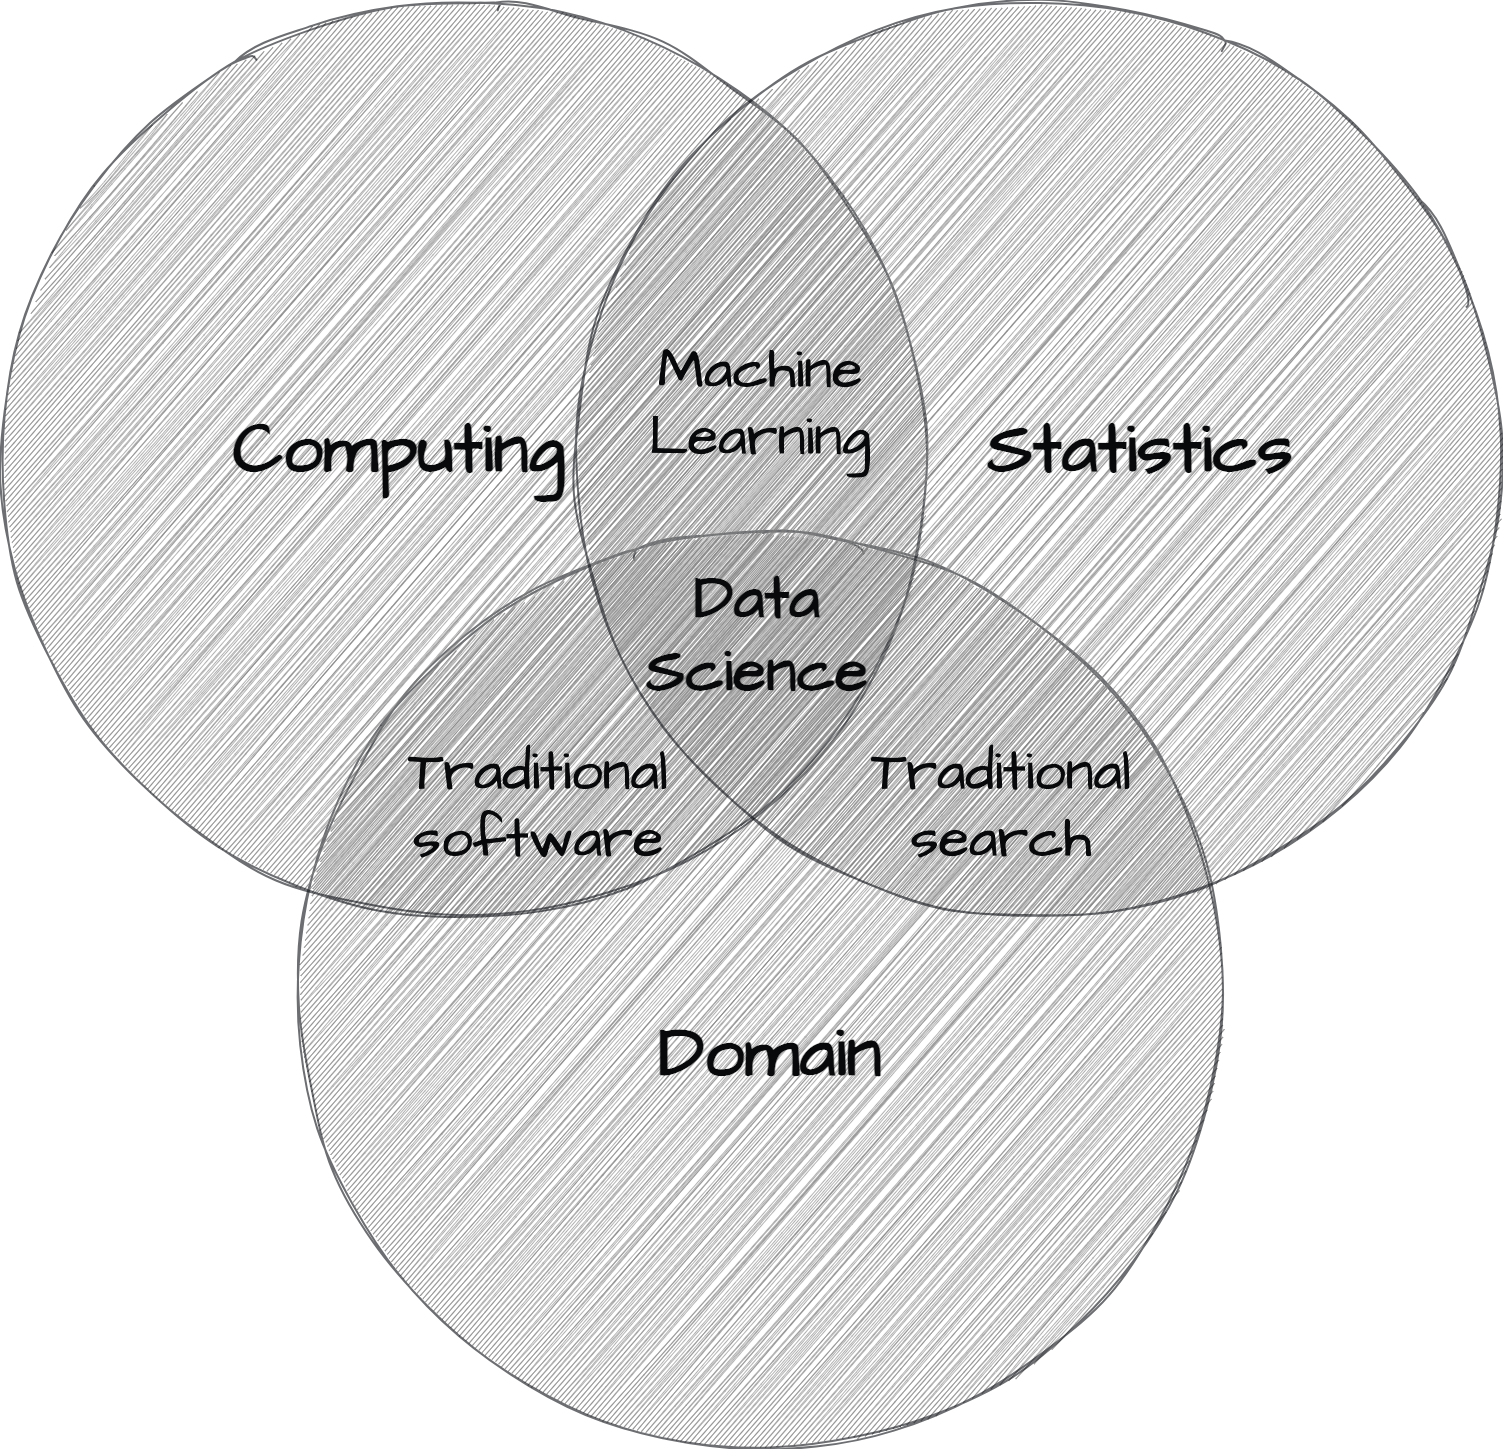
\includegraphics[width=0.5\textwidth,height=\textheight]{figures/text-analysis/ta-ds-venn.drawio.png}

}

\caption{\label{fig-intro-data-science-venn}Data Science Venn Diagram
adapted from
\href{http://drewconway.com/zia/2013/3/26/the-data-science-venn-diagram}{Drew
Conway}.}

\end{figure}

The \textbf{computing skills} component of data science is the ability
to write code to perform the data analysis process. This is the primary
approach for working with data at scale. The \textbf{statistical
knowledge} component of data science is the ability to apply statistical
methods to data to derive insight. \textbf{Domain expertise} provides
researchers insight at key junctures in the development of a research
project and aid researchers in evaluating results.

This triad of skills in combination with reproducible research practices
is the foundational toolbelt of data science
(\protect\hyperlink{ref-Hicks2019}{Hicks and Peng 2019}).
\textbf{Reproducible research}\index{reproducible research} entails the
use of computational tools to automate the process of data analysis.
This automation is achieved by writing code that can be executed to
replicate the data analysis. This code can then be shared through code
sharing repositories, such as GitHub, where it can be viewed,
downloaded, and executed by others. This adds transparency to the
process and allows others to build on previous work. This is in contrast
to traditional approaches where data analysis is performed
(semi-)manually, results are reported in a static document such as a
report or journal article, and the data analysis process is not shared.
This approach is not reproducible because the data analysis process is
not transparent and cannot be replicated. This is problematic because it
is difficult to evaluate the results and build on previous work.
Reproducible research practices are a key component of data science and
are emphasized throughout this book.

\hypertarget{applications-of-data-science}{%
\subsection{Applications of data
science}\label{applications-of-data-science}}

Equipped with the data science toolbelt, the interest in deriving
insight from the available data is now almost ubiquitous. The science of
data has now reached deep into all aspects of life where making sense of
the world is sought. Predicting whether a loan applicant will get a loan
(\protect\hyperlink{ref-Bao2019}{Bao, Lianju, and Yue 2019}), whether a
lump is cancerous (\protect\hyperlink{ref-Saxena2020}{Saxena and
Gyanchandani 2020}), what films to recommend based on your previous
viewing history (\protect\hyperlink{ref-Gomez-Uribe2015}{Gomez-Uribe and
Hunt 2015}), what players a sports team should sign
(\protect\hyperlink{ref-Lewis2004}{Lewis 2004}) all now incorporate a
common set of data analysis tools.

The data science toolbelt also underlies well-known public-facing
language applications. From the language-capable chat applications,
plagiarism detection software, machine translation algorithms, and
search engines, tangible results of quantitative approaches to language
are becoming standard fixtures in our lives, as seen in
Figure~\ref{fig-intro-language-applications}.

\begin{figure}[H]

{\centering 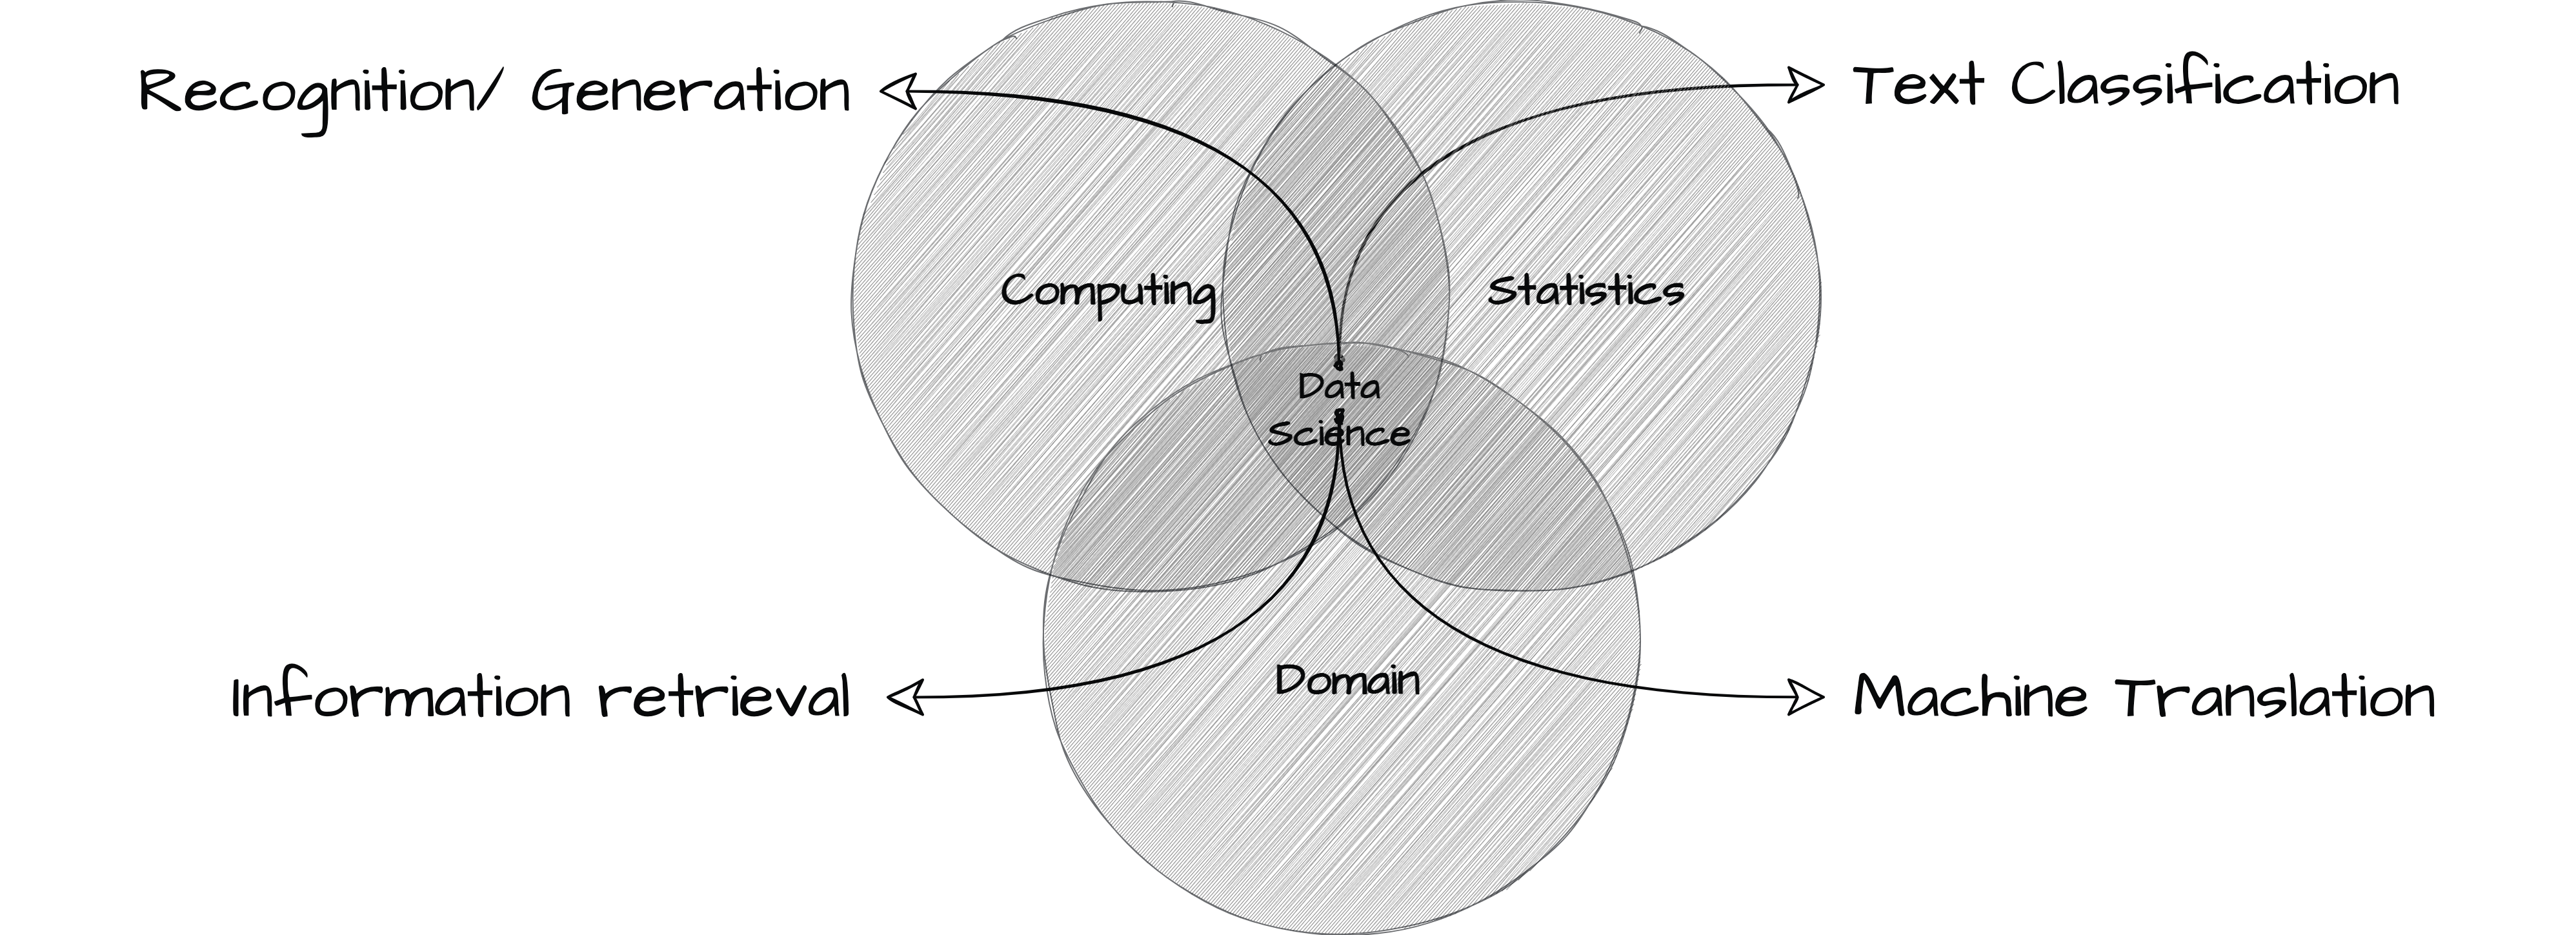
\includegraphics[width=1\textwidth,height=\textheight]{figures/text-analysis/ta-lang-venn.drawio.png}

}

\caption{\label{fig-intro-language-applications}Well-known public-facing
language applications}

\end{figure}

The spread of quantitative data analysis too has taken root in academia.
Even in areas that on first blush don't appear readily approachable in a
quantitative manner, such as fields in the social sciences and
humanities, data science is making important and sometimes disciplinary
changes to the way that academic research is conducted. This textbook
focuses in on a domain that cuts across many of these fields; namely
language. At this point let's turn to quantitative approaches to
language analysis as we work closer to contextualizing text analysis.

\hypertarget{language-analysis}{%
\section{Language analysis}\label{language-analysis}}

Language is a defining characteristic of our species. Since antiquity,
language has attracted interest across disciplines and schools of
thought. In the early 20th century, the development of the rigorous
approach to study of language as a field in its own right took root
(\protect\hyperlink{ref-Campbell2001}{Campbell 2001}), yet a plurality
of theoretical views and methodological approaches remained.
Contemporary linguistics bares this complex history and is far from
theoretically and methodologically unified.

Either based on the tenets of theoretical frameworks and/or the objects
of study of particular fields, approaches to language research vary. On
the one hand some language research commonly applies qualitative
assessment of language structure and/ or use. \textbf{Qualitative
approaches} describe and account for characteristics, or ``qualities'',
that can be observed, but not measured (\emph{e.g.} introspective
methods, ethnographic methods, \emph{etc.})

On the other hand other language research programs employ quantitative
research methods either out of necessity given the object of study
(phonetics, psycholinguistics, \emph{etc.}) or based on theoretical
principles (Cognitive Linguistics, Connectionism, \emph{etc.}).
\textbf{Quantitative approaches} involve measurements of properties of
language that can be observed and measured (\emph{e.g.} frequency of
use, reaction time, \emph{etc.}).

These latter research areas and theoretical paradigms employ methods
that share much of the common data analysis toolbox described in the
previous section. In effect, this establishes a common methodological
language between other language research fields but also with research
outside of linguistics.

However, there is never a one-size-fits all approach to anything --much
less data analysis. And even in quantitative language analysis there is
a key methodological distinction that has downstream effects in terms of
procedure but also in terms of interpretation. The key distinction that
we need to make at this point, which will provide context for our
introduction to quantitative text analysis, comes down to the approach
to collecting language data and the nature of that data. This
distinction is between \textbf{experimental
data}\index{experimental data} and \textbf{observational
data}\index{observational data}.

Experimental approaches start with a intentionally designed hypothesis
and lay out a research methodology with appropriate instruments and a
plan to collect data that shows promise for shedding light on the
validity of the hypothesis. Experimental approaches are conducted under
controlled contexts, usually a lab environment, in which participants
are recruited to perform a language related task with stimuli that have
been carefully curated by researchers to elicit some aspect of language
behavior of interest. Experimental approaches to language research are
heavily influenced by procedures adapted from psychology. This link is
logical as language is a central area of study in cognitive psychology.
This approach looks much like the white-coat science that we made
reference to earlier but, as in most quantitative research, has now
taken advantage of the data analysis toolbelt to collect and organize
much larger quantities of data and conduct statistically more robust
analysis procedures and communicate findings more efficiently.

Observational approaches are a bit more of a mixed bag in terms of the
rationale for the study; they may either start with a testable
hypothesis or in other cases may start with a more open-ended research
question to explore. But a more fundamental distinction between the two
is drawn in the amount of control the researcher has on contexts and
conditions in which the language behavior data to be collected is
produced. Observational approaches seek out records of language behavior
that is produced by language speakers for communicative purposes in
natural(istic) contexts. This may take place in labs (language
development, language disorders, \emph{etc.}), but more often than not,
language is collected from sources where speakers are performing
language as part of their daily lives --whether that be posting on
social media, speaking on the telephone, making political speeches,
writing class essays, reporting the latest news for a newspaper, or
crafting the next novel destined to be a New York Times best-seller.
What is more, data collected from the `wild' varies more in structure
relative to data collected in experimental approaches and requires a
number of steps to prepare the data to sync up with the data analysis
toolbelt.

I liken this distinction between experimental and observational data
collection to the difference between farming and foraging. Experimental
approaches are like farming; the groundwork for a research plan is
designed, much as a field is prepared for seeding, then the researcher
performs as series of tasks to produce data, just as a farmer waters and
cares for the crops, the results of the process bear fruit, data in our
case, and this data is harvested. Observational approaches are like
foraging; the researcher scans the available environmental landscape for
viable sources of data from all the naturally existing sources, these
sources are assessed as to their usefulness and value to address the
research question, the most viable is selected, and then the data is
collected.

The data acquired from both of these approaches have their trade-offs,
just as farming and foraging. Experimental approaches directly elicit
language behavior in highly controlled conditions. This directness and
level of control has the benefit of allowing researchers to precisely
track how particular experimental conditions effect language behavior.
As these conditions are an explicit part of the design and therefore the
resulting language behavior can be more precisely attributed to the
experimental manipulation. The primary shortcoming of experimental
approaches is that there is a level of artificialness to this directness
and control. Whether it is the language materials used in the task, the
task itself, or the fact that the procedure takes place under
supervision the language behavior elicited can diverge quite
significantly from language behavior performed in natural communicative
settings. Observational approaches show complementary strengths and
shortcomings.

Whereas experimental approaches may diverge from natural language use,
observational approaches strive to identify and collected language
behavior data in natural, uncontrolled, and unmonitored contexts, as
seen in Figure~\ref{fig-data-collection-methods}. In this way
observational approaches do not have to question to what extent the
language behavior data is or is not performed as a natural communicative
act. On the flipside, the contexts in which natural language
communication take place are complex relative to experimental contexts.
Language collected from natural contexts are nested within the complex
workings of a complex world and as such inevitably include a host of
factors and conditions which can prove challenging to disentangle from
the language phenomenon of interest but must be addressed in order to
draw reliable associations and conclusions.

\begin{figure}[H]

{\centering 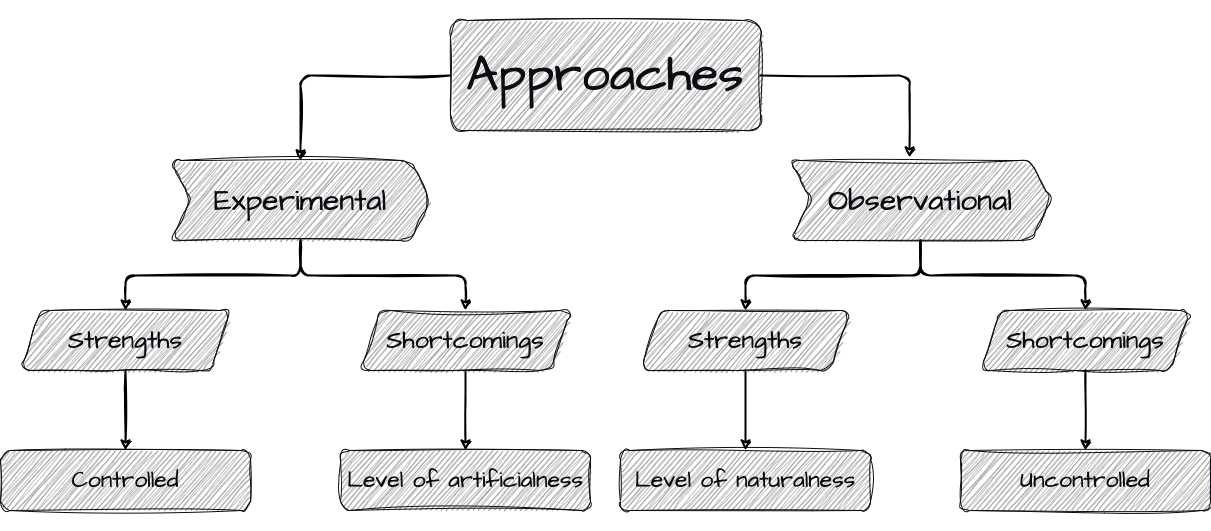
\includegraphics[width=4.04in,height=\textheight]{figures/text-analysis/ta-data-collection-methods.drawio.png}

}

\caption{\label{fig-data-collection-methods}Trade-offs between
experimental and observational data collection methods.}

\end{figure}

The upshot, then, is twofold: (1) data collection methods matter for
research design and interpretation and (2) there is no single best
approach to data collection, each have their strengths and shortcomings.
In the ideal, a robust science of language will include insight from
both experimental and observational approaches
(\protect\hyperlink{ref-Gilquin2009}{Gilquin and Gries 2009}). And
evermore there is greater appreciation for the complementary nature of
experimental and observational approaches and a growing body of research
which highlights this recognition.

\begin{tcolorbox}[enhanced jigsaw, rightrule=.15mm, leftrule=.75mm, opacityback=0, arc=.35mm, colback=white, breakable, toprule=.15mm, bottomrule=.15mm, left=2mm]

\textbf{\faIcon{file-alt} Case study}

Manning (\protect\hyperlink{ref-Manning2003}{2003}) discusses the use of
probabilistic models in syntax to account for the variability in
language usage and the presence of both hard and soft constraints in
grammar. The paper touches on the statistical methods in text analysis,
the importance of distinguishing between external and internal language,
and the limitations of Generative Grammar. Overall, the paper suggests
that usage-based and formal syntax can learn from each other to better
understand language variation and change.

\end{tcolorbox}

Given their particular trade-offs observational data is often used as an
exploratory starting point to help build insight and form predictions
that can then be submitted to experimental conditions. In this way,
studies based on observational data serve as an exploratory tool to
gather a better and more externally valid view of language use which can
then serve to make prediction that can be explored with more precision
in an experimental paradigm. However, this is not always the case;
observational data is also often used in hypothesis-testing contexts as
well. And furthermore, some in some language-related fields, a
hypothesis-testing is not the approach for deriving knowledge and
insight.

\hypertarget{text-analysis}{%
\section{Text analysis}\label{text-analysis}}

In a nutshell, \textbf{text analysis}\index{Text analysis} is the
process of leveraging the data science toolbelt to derive insight from
textual data collected through observational methods. In the next
subsections, I will unpack this definition and discuss the primary
components that make up text analysis including research appoaches and
technical implementation, as well as practical applications.

\hypertarget{approaches}{%
\subsection{Approaches}\label{approaches}}

Text analysis is a multifacited research methodology. It can be used use
facilitate the qualitative exploration of smaller, human-digestable
textual information, but is more often employed quantitatively to bring
to the surface patterns and relationships in large samples of textual
data that would be otherwise difficult, if not impossible, to identify
manually.

Text being text, there are a series of \textbf{data prepration} steps
that must be taken to ready the data for analysis. In addition to
collecting the data, the data must be organized, cleaned, and
transformed into a format that is amenable to statistical analysis.

The statistical and evaluative approach employed in the analysis is
dependent on the aim of the research. For research aimed at exploring
and uncovering patterns and relationships in a data-driven manner,
\textbf{Exploratory Data Analysis} (EDA) is employed. EDA combines
descriptive statistics, visualizations, and statistical learning methods
in an iterative and interactive way to provide the researcher the
ability to identify patterns and relationships and to evaluate whether
and why they are meaningful.

\textbf{Predictive Data Analysis} (PDA), applied in research for outcome
prediction, is a supervised machine learning task. It uses feature sets
to predict an outcome variable. Its primary evaluation metric is the
prediction accuracy on new data. However, for many text analysis tasks,
human interpretation is crucial to provide context and assess the
significance of the results.

Research aimed at explaining relationships between variables and the
population from which the sample was drawn will adopt an
\textbf{Inferential Data Analysis} (IDA) approach. IDA is a
theory-driven process that employs statistical models for hypothesis
testing. The extent to which the results can be confidently generalized
to the population is the primary evaluation metric.

As we see, text analysis can be used for a variety of purposes; from
data-driven exploration and discovery to hypothesis testing and
generalization.

\hypertarget{implementation}{%
\subsection{Implementation}\label{implementation}}

To ensure that the results of text analysis projects are replicable and
transparent, programming strategies play an integral role at each stage
of the implementation of a research project. While there are a number of
programming languages that can be used for text analysis, R widely
adopted in linguistics research. R is a free and open-source programming
language that is specifically designed for statistical computing and
graphics. It has a large and active community of users and developers,
and a robust ecosystem of packages which make it a powerful and flexible
language that is well-suited for core text analysis tasks: data
collection, organization, transformation, analysis, and visualization.
When combined with Quarto for literate programming and GitHub for
version control and collaboration, R provides a robust and reproducible
workflow for text analysis.

\hypertarget{applications}{%
\subsection{Applications}\label{applications}}

So what are some applications of text analysis? Most public facing
applications stem from Computational Linguistic research, often known as
\textbf{Natural Language Processing} (NLP) by practitioners. Whether it
be using search engines, online translators, submitting your paper to
plagiarism detection software, \emph{etc.} many of the text analysis
methods we will cover are at play.

\begin{tcolorbox}[enhanced jigsaw, rightrule=.15mm, leftrule=.75mm, opacityback=0, arc=.35mm, colback=white, breakable, toprule=.15mm, bottomrule=.15mm, left=2mm]

\textbf{\faIcon{lightbulb} Consider this}

What are some other public facing applications of text analysis that you
are aware of?

\end{tcolorbox}

In academia the use of quantitative text analysis is even more
widespread, despite the lack of public fanfare. In linguistics, text
analysis is applied to a wide range of topics and research questions in
both theoretical and applied subfields, as seen in
Example~\ref{exm-linguistic-theory} and
Example~\ref{exm-linguistic-applied}.

\begin{example}[]\protect\hypertarget{exm-linguistic-theory}{}\label{exm-linguistic-theory}

Theoretical linguistics

\begin{itemize}
\tightlist
\item
  Hay (\protect\hyperlink{ref-Hay2002}{2002}) use a corpus study to
  investigate the role of frequency and phonotatics in affix ordering in
  English.
\item
  Riehemann (\protect\hyperlink{ref-Riehemann2001}{2001}) explores the
  extent to which idiomatic expressions (\emph{e.g.} `raise hell') are
  lexical or syntactic units.
\item
  Bresnan (\protect\hyperlink{ref-Bresnan2007a}{2007}) investigate the
  claim that possessed deverbal nouns in English (\emph{e.g.} `the
  city's destruction') are subject to a syntactic constraint that
  requires the possessor to be affected by the action denoted by the
  deverbal noun.
\end{itemize}

\end{example}

\begin{example}[]\protect\hypertarget{exm-linguistic-applied}{}\label{exm-linguistic-applied}

Applied linguistics

\begin{itemize}
\tightlist
\item
  Wulff, Stefanowitsch, and Gries
  (\protect\hyperlink{ref-Wulff2007}{2007}) explore differences between
  British and American English at the lexico-syntactic level in the
  \emph{into}-causative construction (\emph{e.g.} `He tricked me into
  employing him.').
\item
  Eisenstein et al. (\protect\hyperlink{ref-Eisenstein2012}{2012}) track
  the geographic spread of neologisms (\emph{e.g.} `bruh', `af',
  '-\_\_-') from city to city in the United States using Twitter data
  collected between 6/2009 and 5/2011.
\item
  Bychkovska and Lee (\protect\hyperlink{ref-Bychkovska2017}{2017})
  investigates possible differences between L1-English and L1-Chinese
  undergraduate students' use of lexical bundles, multiword sequences
  which are extended collocations (\emph{e.g.} `as the result of'), in
  argumentative essays.
\item
  Jaeger and Snider (\protect\hyperlink{ref-Jaeger2007}{2007}) use a
  corpus study to investigate the phenomenon of syntactic persistence,
  the increased tendency for speakers to use a particular syntactic form
  over an alternate when the syntactic form has been recently processed.
\item
  Voigt et al. (\protect\hyperlink{ref-Voigt2017}{2017}) explore
  potential racial disparities in officer respect in police body camera
  footage.
\item
  Olohan (\protect\hyperlink{ref-Olohan2008}{2008}) investigate the
  extent to which translated texts differ from native texts do to
  `explicitation'.
\end{itemize}

\end{example}

So too, text analysis is used in a variety of other fields where insight
from language is sought, as seen in Example~\ref{exm-other-fields}.

\begin{example}[]\protect\hypertarget{exm-other-fields}{}\label{exm-other-fields}

Language-related fields

\begin{itemize}
\tightlist
\item
  Kloumann et al. (\protect\hyperlink{ref-Kloumann2012}{2012}) explore
  the extent to which languages are positively, neutrally, or negatively
  biased.
\item
  Mosteller and Wallace (\protect\hyperlink{ref-Mosteller1963}{1963})
  provide a method for solving the authorship debate surrounding The
  Federalist papers.
\item
  Conway et al. (\protect\hyperlink{ref-Conway2012}{2012}) investigate
  whether the established drop in language complexity of rhetoric in
  election seasons is associated with election outcomes.
\end{itemize}

\end{example}

\begin{tcolorbox}[enhanced jigsaw, rightrule=.15mm, leftrule=.75mm, opacityback=0, arc=.35mm, colback=white, breakable, toprule=.15mm, bottomrule=.15mm, left=2mm]

\textbf{\faIcon{lightbulb} Consider this}

Language is a key component of human communication and interaction. What
are some other areas of research in and outside linguistics that you
think could be explored using text analysis methods?

\end{tcolorbox}

These studies in Examples \ref{exm-linguistic-theory},
\ref{exm-linguistic-applied}, and \ref{exm-other-fields} are just a few
illustrations of the contributions of text analysis as the primary
method to gain a deeper understanding of language structure, function,
variation, and acquisition. As a method, however, text analysis can also
be used to support other research methods. For example, text analysis
can be used collect data, generate authentic materials, provide
linguistic annotation, to generate hypotheses, for either qualitative
and/ or quantitative approaches. Together these efforts contribute to a
more robust language science by incorporating externally valid data and
providing methodological triangulation
(\protect\hyperlink{ref-Francom2022}{Francom 2022}).

In sum, the applications highlighted in this section underscore the
versatility of text analysis as a research method. Whether it be in the
public sphere or in academia, text analysis methods furnish a set of
powerful tools for gaining insight from language data.

\hypertarget{summary}{%
\section*{Summary}\label{summary}}
\addcontentsline{toc}{section}{Summary}

\markright{Summary}

In this chapter I started with some general observations about the
difficulty of making sense of a complex world. The standard approach to
overcoming inherent human limitations in sense making is science. In the
21st century the toolbelt for doing scientific research and exploration
has grown in terms of the amount of data available, the statistical
methods for analyzing the data, and the computational power to manage,
store, and share the data, methods, and results from quantitative
research. The methods and tools for deriving insight from data have made
significant inroads in and outside academia, and increasingly figure in
the quantitative investigation of language. Text analysis is a
particular branch of this enterprise based on observational data from
real-world language and is used in a wide variety of fields.

In the end I hope that you enjoy this exploration into text analysis.
Although the learning curve at times may seem steep --the experience you
will gain will not only improve your data literacy, research skills, and
programmings skills but also enhance your appreciation for the richness
of human language and its important role in our everyday lives.

\hypertarget{actitivies}{%
\section*{Actitivies}\label{actitivies}}
\addcontentsline{toc}{section}{Actitivies}

\markright{Actitivies}

The following activities build on your introduction to R and Quarto in
the previous chapter. In these activities you will uncover more features
offered by Quarto which will enhance your ability to produce
comprehensive reproducible research documents. You will apply the
capabilities of Quarto in a practical context conveying the objectives
and key discoveries from a primary research article.

\begin{tcolorbox}[enhanced jigsaw, rightrule=.15mm, leftrule=.75mm, opacityback=0, arc=.35mm, colback=white, breakable, toprule=.15mm, bottomrule=.15mm, left=2mm]

\textbf{\faIcon{file-code} Recipe}

\textbf{What}:
\href{https://qtalr.github.io/qtalrkit/articles/recipe-.html}{Literate
programming II}\\
\textbf{How}: Read Recipe 1 and participate in the Hypothes.is online
social annotation.\\
\textbf{Why}: To explore additional functionality in Quarto: numbered
sections, table of contents, in-line citations and a document-final
references list, and cross-referenced tables and figures.

\end{tcolorbox}

\begin{tcolorbox}[enhanced jigsaw, rightrule=.15mm, leftrule=.75mm, opacityback=0, arc=.35mm, colback=white, breakable, toprule=.15mm, bottomrule=.15mm, left=2mm]

\textbf{\faIcon{flask} Lab}

\textbf{What}: \href{https://github.com/qtalr/lab-1}{Literate
programming II}\\
\textbf{How}: Clone, fork, and complete the steps in Lab 1.\\
\textbf{Why}: To put into practice Quarto functionality to communicate
the aim(s) and main finding(s) from a primary research article and to
interpret a related plot.

\end{tcolorbox}

\hypertarget{questions}{%
\section*{Questions}\label{questions}}
\addcontentsline{toc}{section}{Questions}

\markright{Questions}

\begin{tcolorbox}[enhanced jigsaw, rightrule=.15mm, leftrule=.75mm, opacityback=0, arc=.35mm, colback=white, breakable, toprule=.15mm, bottomrule=.15mm, left=2mm]

\textbf{Conceptual questions}

\begin{itemize}
\tightlist
\item
  How has scientific research and exploration changed in the 21st
  century?
\item
  What are the three basic skill sets that make up the data science
  toolbelt?
\item
  What are the benefits of reproducible research in data science?
\item
  Explain the trade-offs between experimental and observational data
  collection methods.
\item
  What is text analysis and how is it used in various fields?
\item
  Identify research in an area of interest in linguistics that has taken
  a quantitative approach to text analysis.
\item
  In your own words, define literate programming?
\item
  What are the benefits of literate programming?
\item
  What are the benefits of using R and Quarto for literate programming?
\end{itemize}

\end{tcolorbox}

\begin{tcolorbox}[enhanced jigsaw, rightrule=.15mm, leftrule=.75mm, opacityback=0, arc=.35mm, colback=white, breakable, toprule=.15mm, bottomrule=.15mm, left=2mm]

\textbf{Technical exercises}

\begin{itemize}
\tightlist
\item
  Create a literate programming document in Quarto. Edit the yaml header
  to reflect details of the work and add your work with the data types
  in R to code chunks. Add, commit, and push the project to GitHub.
\item
  In the Quarto document, explore using R to create vectors and explore
  their properties.
\item
  Explore the following resources and with the goal to identify a
  quantitative text analysis project. \href{https://rpubs.com/}{Rpubs},
  \href{https://github.com}{GitHub},
  \href{https://datacamp.com}{DataCamp},
  \href{https://kaggle.com}{Kaggle},
  \href{https://r-bloggers.com}{R-bloggers}.
\item
  \faIcon{wrench} \ldots{} more to come \ldots{}
\end{itemize}

\end{tcolorbox}

\part{Foundations}

Before working on the specifics of a data project, it is important to
establish a fundamental understanding of the characteristics of each of
the levels in the ``Data, Information, Knowledge, and Insight Hierarchy
(DIKI)'' (see Figure~\ref{fig-diki-hierarchy}) and the roles each of
these levels have in deriving insight from data. In
Chapter~\ref{sec-understanding-data} we will explore the Data and
Information levels drawing a distinction between two main types of data
(populations and samples) and then cover how data is structured and
transformed to generate information (datasets) that is fit for
statistical analysis. In Chapter~\ref{sec-approaching-analysis} I will
outline the importance and distinct types of statistical procedures
(descriptive and analytic) that are commonly used in text analysis.
Chapter~\ref{sec-framing-research} aims to tie these concepts together
and cover the required steps for preparing a research blueprint to
conduct an original text analysis project.

\hypertarget{sec-understanding-data}{%
\chapter{Understanding data}\label{sec-understanding-data}}

\begin{tcolorbox}[enhanced jigsaw, leftrule=.75mm, title=\textcolor{quarto-callout-tip-color}{\faLightbulb}\hspace{0.5em}{Draft}, coltitle=black, opacityback=0, titlerule=0mm, arc=.35mm, bottomtitle=1mm, opacitybacktitle=0.6, colframe=quarto-callout-tip-color-frame, rightrule=.15mm, toptitle=1mm, left=2mm, colback=white, breakable, toprule=.15mm, bottomrule=.15mm, colbacktitle=quarto-callout-tip-color!10!white]

Ready for review.

\end{tcolorbox}

\begin{quote}
The goal is to turn data into information, and information into insight.

--- Carly Fiorina
\end{quote}

\begin{tcolorbox}[enhanced jigsaw, rightrule=.15mm, leftrule=.75mm, opacityback=0, arc=.35mm, colback=white, breakable, toprule=.15mm, bottomrule=.15mm, left=2mm]

\textbf{\faIcon{list-alt} Outcomes}

\begin{itemize}
\tightlist
\item
  Describe the difference between data and information.
\item
  Understand how the tidy approach to data organization can enhance the
  quality and usability of data.
\item
  Articulate the importance of documentation in promoting reproducible
  research.
\end{itemize}

\end{tcolorbox}

In this chapter, the groundwork is laid for deriving insights from text
analysis by focusing on content and structure of data and information.
The concepts of populations and samples are introduced, highlighting
their similarities and key differences. Connecting these topics to text
analysis, language samples, or corpora, are explored, discussing their
types, sources, formats, and ethical considerations. Subsequently, key
concepts in creating information from data, such as organization and
transformation, are examined. Finally, the importance of documentation
in quantitative research is emphasized through addressing data origin
and data dictionaries.

\begin{tcolorbox}[enhanced jigsaw, rightrule=.15mm, leftrule=.75mm, opacityback=0, arc=.35mm, colback=white, breakable, toprule=.15mm, bottomrule=.15mm, left=2mm]

\textbf{\faIcon{terminal} Swirl lesson}

\textbf{What}: \href{https://github.com/qtalr/swirl}{Objects, Packages
and functions}\\
\textbf{How}: In the R Console pane load \texttt{swirl}, run
\texttt{swirl()}, and follow prompts to select the lesson.\\
\textbf{Why}: To introduce you to the main types of objects in R and to
understand the role and use of functions and packages in R programming.

\end{tcolorbox}

\hypertarget{sec-ud-data}{%
\section{Data}\label{sec-ud-data}}

Data is data, right? The term `data' is so common in popular vernacular
it is easy to assume we know what we mean when we say `data'. But as in
most things, where there are common assumptions there are important
details that require more careful consideration. Let's turn to the first
key distinction that we need to make to start to break down the term
`data': the difference between populations and samples.

\hypertarget{sec-ud-populations}{%
\subsection{Populations}\label{sec-ud-populations}}

The first thing that comes to many people's mind when the term
population is used is human populations (derived from Latin `populus').
Say for example we pose the question --What's the population of
Milwuakee? When we speak of a population in these terms we are talking
about the total sum of individuals living within the geographical
boundaries of Milwaukee. In concrete terms, a
\index{population}\textbf{population} an idealized set of objects or
events in reality which share a common characteristic or belong to a
specific category. The term to highlight here is idealized. Although we
can look up the US Census report for Milwaukee and retrieve a figure for
the population, this cannot truly be the population. Why is that? Well,
whatever method that was used to derive this numerical figure was surely
incomplete. If not incomplete, by the time someone recorded the figure
some number of residents of Milwaukee moved out, moved in, were born, or
passed away. In either case, this example serves to point out that
populations are not fixed and are subject to change over time.

Likewise when we talk about populations in terms of language we dealing
with an idealized aspect of linguistic reality. Let's take the words of
the English language as an analog to our previous example population. In
this case the words are the people and English is the grouping
characteristic. Just as people, words move out, move in, are born, and
pass away. Any compendium of the words of English at any moment is
almost instananeously incomplete. This is true for all populations, save
those relatively rare cases in which the grouping characteristics select
a narrow slice of reality which is objectively measurable and whose
membership is fixed (the complete works of Shakespeare, for example).

In sum, (most) populations are amorphous moving targets. We subjectively
hold them to exist, but in practical terms we often cannot nail down the
specifics of populations. So how do researchers go about studying
populations if they are theoretically impossible to access directly? The
strategy employed is called sampling.

\hypertarget{sec-ud-samples}{%
\subsection{Samples}\label{sec-ud-samples}}

A \index{sample}\textbf{sample} is the product of a subjective process
of selecting a finite set of observations from an idealized population
with the goal of capturing the relevant characteristics of the target
population. The \textbf{degree of representativeness}
\index{sample!representativeness} of a sample is the extent to which the
sample reflects the characteristics of the population. The degree of
representativeness is crucial for research as it directly impacts of any
findings based on the sample.

To maximize the representativeness of a sample, researchers employ a
variety of strategies. One of the first and sometimes the easiest
strategy is to increase the \index{sample size}\textbf{sample size}. A
larger sample will always be more representative than a smaller sample.
Sample size, however, is often not enough. It is not hard to imagine a
large sample which by chance captures only a subset of the features of
the population. Another step to enhance sample representativeness is to
apply \textbf{random sampling}. Together a large random sample has an
even better chance of reflecting the main characteristics of the
population better than a large or random sample. But, random as random
is, we still run the risk of acquiring a skewed sample (\emph{i.e.} a
sample with low representativeness).

To help mitigate these issues, there are two more strategies that can be
applied to improve sample representativeness. Note, however, that while
size and random samples can be applied to any sample with few
assumptions about internal characteristics of the population, these next
two strategies require decisions depend on the presumed internal
characteristics of the population.

The first of these more informed sampling strategies is called
\textbf{stratified sampling}. Stratified samples make (educated)
assumptions about sub-components within the population of interest. With
these sub-populations in mind, large random samples are acquired for
each sub-population, or strata. At a minimum, stratified samples can be
no less representative than random sampling alone, but the chances that
the sample is better increases. Can there be problems in the approach?
Yes, and on two fronts. First knowledge of the internal components of a
population are often based on a limited or incomplete knowledge of the
population (remember populations are idealized). In other words, strata
are selected subjectively by researchers using various heuristics some
of which are based on some sense of `common knowledge'.

The second front on which stratified sampling can err concerns the
relative sizes of the sub-components relative to the whole population,
which is known as \textbf{balance}. Even if the relevant sub-components
are identified, their relative size adds another challenge which
researchers must address in order to maximize the representativeness of
a sample.

Together, large randomly selected and balanced stratified samples set
the benchmark for sampling. However, hitting this ideal is not always
feasible. There are situations where sizeable samples are not
accessible. Alternatively, there may be instances where the population
or its strata are not well understood. In such scenarios, researchers
have to work with the most suitable sample they can obtain given the
limitations of their research project.

\hypertarget{corpora}{%
\subsection{Corpora}\label{corpora}}

A key feature of a sample is that it is purposely selected to model a
target population. In text analysis, a purposely sampled collection of
texts, of the type defined here, is known as a \textbf{corpus}
(\emph{pl.} corpora). A set of texts or documents which have not been
selected purposely lack a \textbf{sampling frame}, and therefore is not
a corpus. The sampling frame, hence the populations modeled, in any
given corpus will vary. It is key to vet corpora to ensure that the
resource's sampling frame and the research project's target populations
align as closely as possible to safeguard the integrity of research
findings later in the research process.

\begin{tcolorbox}[enhanced jigsaw, rightrule=.15mm, leftrule=.75mm, opacityback=0, arc=.35mm, colback=white, breakable, toprule=.15mm, bottomrule=.15mm, left=2mm]

\textbf{\faIcon{lightbulb} Consider this}

\begin{figure}[H]

\begin{minipage}[t]{0.48\linewidth}
The `Standard Sample of Present-Day American English' (known commonly as
the Brown Corpus) is widely recognized as one of the first large,
machine-readable corpora. Compiled by Kucera and Francis
(\protect\hyperlink{ref-Kucera1967}{1967}), the corpus is comprised of
1,014,312 words from edited English prose published in the United States
in 1961.Given the sampling frame for this corpus visualized in
Figure~\ref{fig-ud-brown-distribution}, can you determine what language
population this corpus aims to represent? What types of research might
this corpus support or not support?\end{minipage}%
%
\begin{minipage}[t]{0.03\linewidth}
~\end{minipage}%
%
\begin{minipage}[t]{0.48\linewidth}

\begin{figure}[H]

{\centering 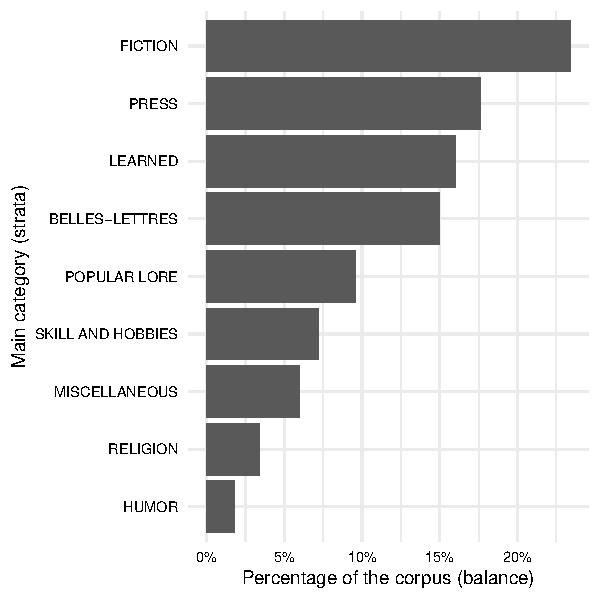
\includegraphics{understanding-data_files/figure-pdf/fig-ud-brown-distribution-1.pdf}

}

\caption{\label{fig-ud-brown-distribution}Overview of the sampling frame
of the Brown Corpus.}

\end{figure}

\end{minipage}%

\end{figure}

\end{tcolorbox}

\hypertarget{types}{%
\subsubsection{Types}\label{types}}

Let's take a look at some key characteristics, attributes, and features
that distinguish corpora.

\hypertarget{reference}{%
\paragraph{Reference}\label{reference}}

The least common and most ambitious corpus resources are those which aim
to model the characteristics of a language population. These are known
as \textbf{reference corpora}. These are projects designed with wide
sampling frames, and require significant investments of time in corpus
design and implementation (and continued development) that are usually
undertaken by research teams (\protect\hyperlink{ref-Adel2020}{Ädel
2020}).

The \href{https://www.anc.org/}{American National Corpus (ANC)} or the
\href{http://www.natcorp.ox.ac.uk/}{British National Corpus (BNC)} are
corpora which aim to model the general characteristics of a variety of
the English language, the former of American English and the later
British English. Reference corpora exist for other languages as well:
Spanish \href{http://corpus.rae.es/creanet.html}{Reference Corpus of
Present-Day Spanish (CREA)}, German
\href{https://www.ids-mannheim.de/digspra/kl/projekte/korpora/}{The
German Reference Corpus (DeReKo)}, Turkish
\href{https://www.tnc.org.tr/}{Turkish National Corpus (TNC)}, and many
others.

\begin{tcolorbox}[enhanced jigsaw, rightrule=.15mm, leftrule=.75mm, opacityback=0, arc=.35mm, colback=white, breakable, toprule=.15mm, bottomrule=.15mm, left=2mm]

\textbf{\faIcon{lightbulb} Consider this}

Of note is the fact that, at present, most of the world's languages lack
reference corpus resources, or any corpus resources whatsoever.
``Low-resourced'' languages are often less studied, resource scarce,
less available in born-digital formats, etc.
(\protect\hyperlink{ref-Magueresse2020}{Magueresse, Carles, and
Heetderks 2020}).

Visit the
\href{https://www.clarin.eu/resource-families/reference-corpora}{Clarin
overview} on reference corpora and then visit
\href{https://lremap.elra.info/}{LRE Map}. Can you find a reference
corpus for a language you speak or are interested in studying? If not,
consider what can be done to address this gap in the research community.

\end{tcolorbox}

\hypertarget{specialized}{%
\paragraph{Specialized}\label{specialized}}

\textbf{Specialized corpora} aim to represent more specific populations.
The population may be defined either by modality, genre, time, location,
or speaker-oriented characteristics, or some combination thereof. What
specialized corpora lack in breadth of coverage, they make up for in
depth of coverage by providing a more targeted representation of
specific language populations.

The
\href{https://www.linguistics.ucsb.edu/research/santa-barbara-corpus}{Santa
Barbara Corpus of Spoken American English (SBCSAE)}, as you can imagine
from the name of the resource, aims to model spoken American English. No
claim to written English is included. There are even more specific types
of corpora which attempt to model other types of sub-populations such as
\href{https://www.coventry.ac.uk/research/research-directories/current-projects/2015/british-academic-written-english-corpus-bawe/}{academic
writing},
\href{https://www.clarin.eu/resource-families/cmc-corpora}{computer-mediated
communication (CMC)}, language use in specific
\href{http://ice-corpora.net/ice/index.html}{regions of the world}, a
\href{https://www.wgtn.ac.nz/lals/resources/corpora-default/corpora-wsc}{country},
a \href{https://cesa.arizona.edu}{region of a country}, \emph{etc}.

\begin{tcolorbox}[enhanced jigsaw, rightrule=.15mm, leftrule=.75mm, opacityback=0, arc=.35mm, colback=white, breakable, toprule=.15mm, bottomrule=.15mm, left=2mm]

\textbf{\faIcon{lightbulb} Consider this}

\begin{figure}[H]

\begin{minipage}[t]{0.58\linewidth}
Grieve, Nini, and Guo (\protect\hyperlink{ref-Grieve2018}{2018})
compiled a 8.9 billion-word corpus of geotagged posts from Twitter
between 2013-2014 in the United States. The authors provide a
\href{https://isogloss.shinyapps.io/isogloss/}{search interface} to
explore relationship between lexical usage and geographic location.
Explore this corpus searching for terms related to slang (``hella'',
``wicked''), geographical (``mountain'', ``river''), meteorological
(``snow'', ``rain''), and/ or any other term types. What types of
patterns do you find? What are the benefits and/ or limitations of this
type of data and/ or interface?\end{minipage}%
%
\begin{minipage}[t]{0.03\linewidth}
~\end{minipage}%
%
\begin{minipage}[t]{0.39\linewidth}

\begin{figure}[H]

{\centering 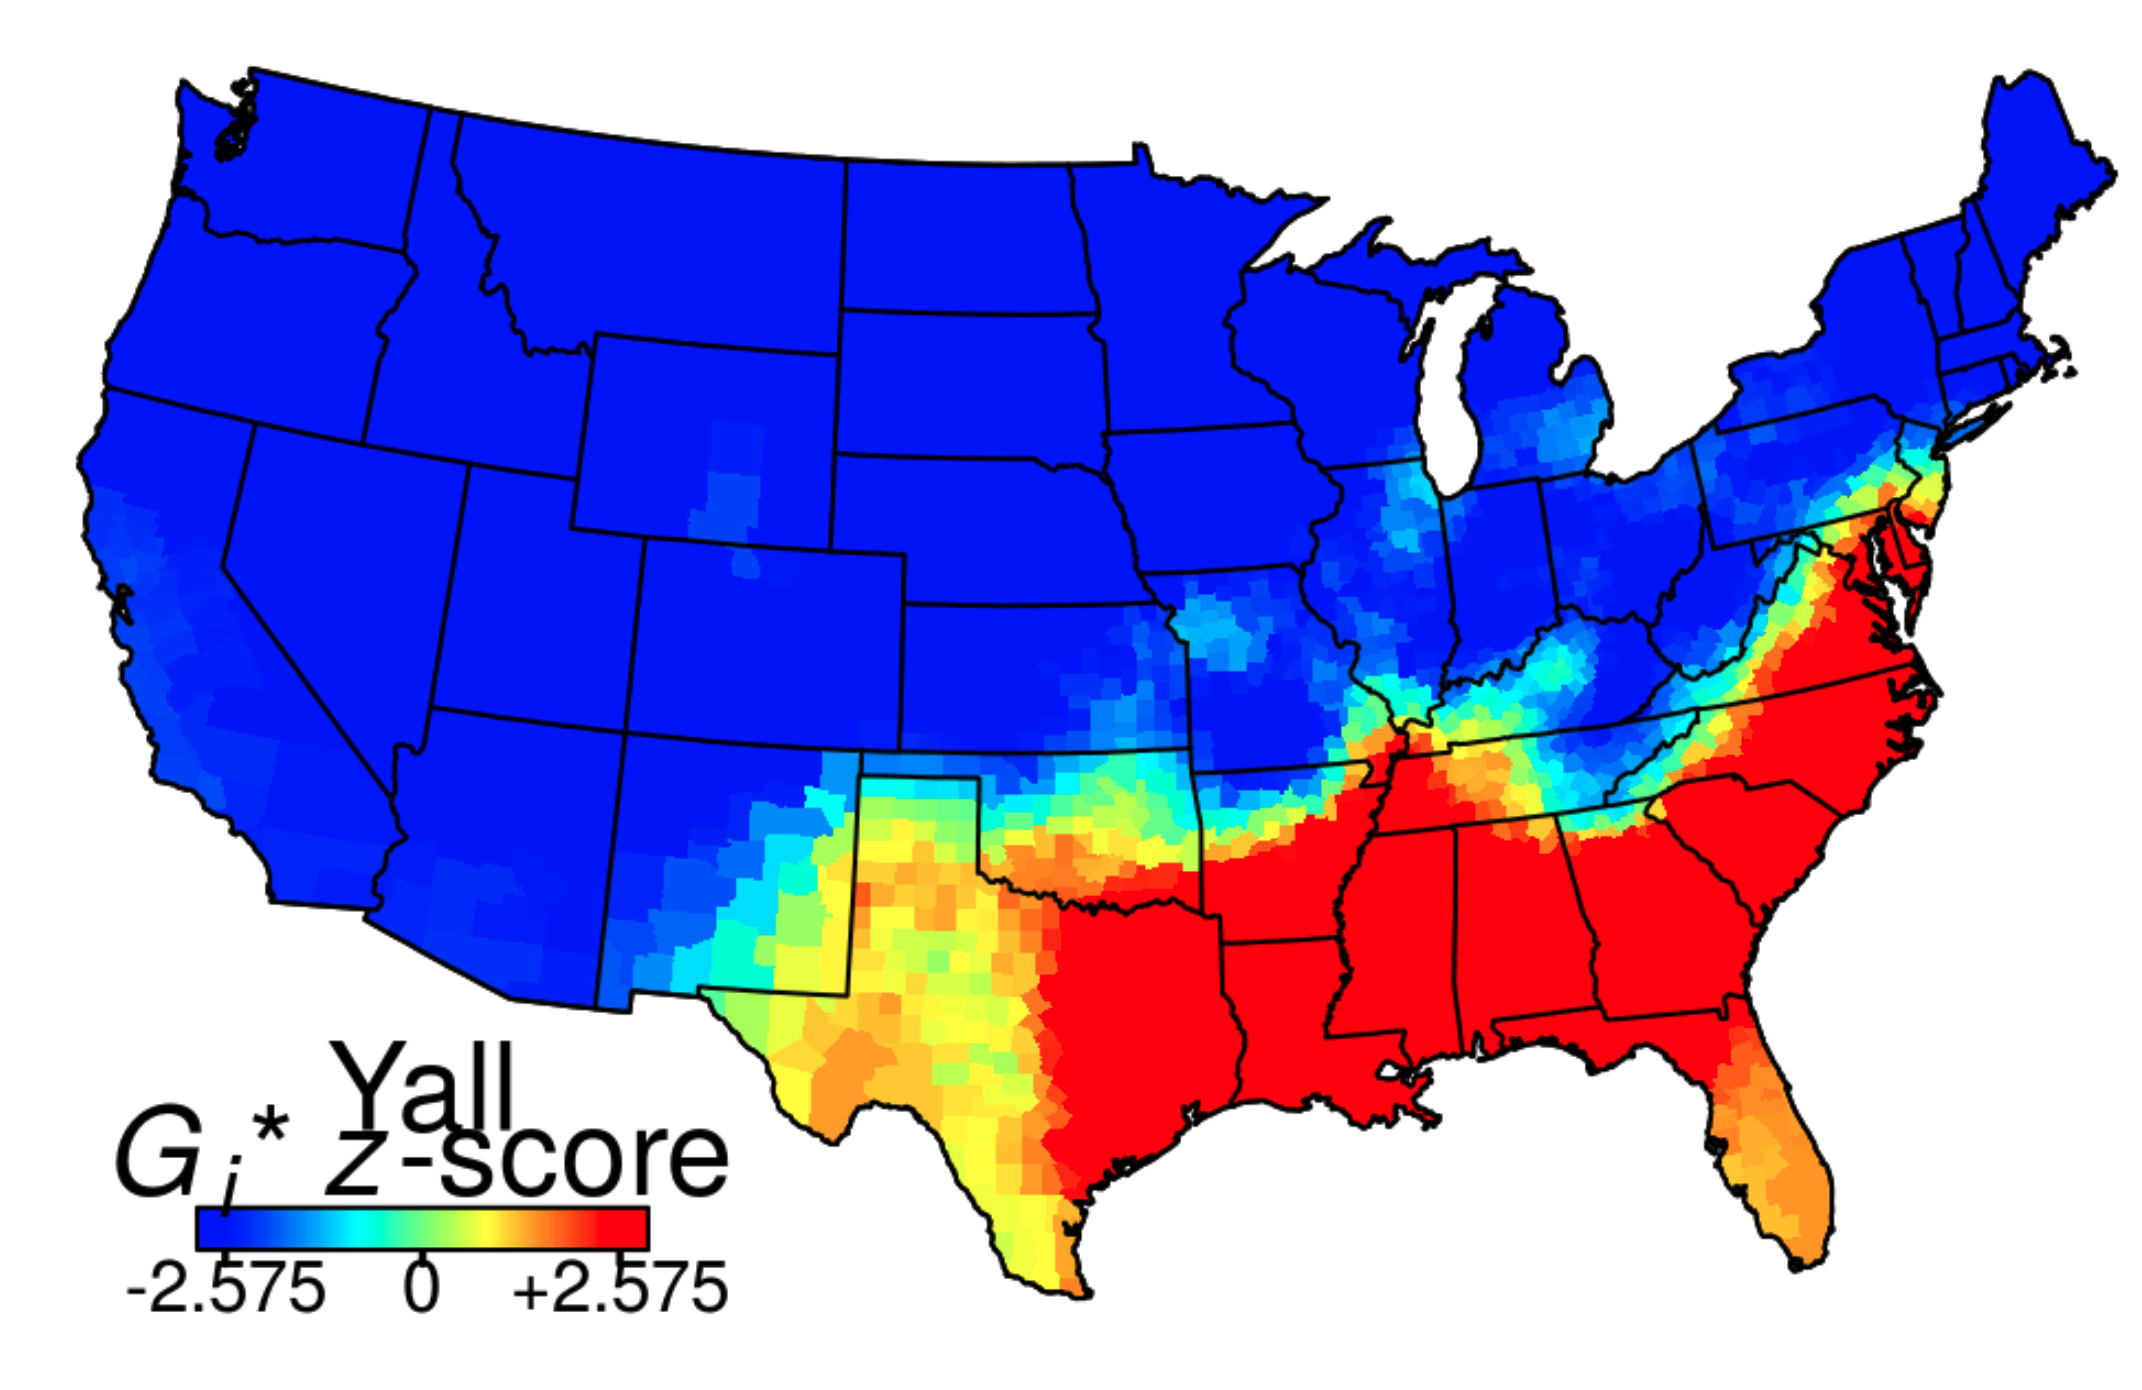
\includegraphics[width=0.8\textwidth,height=\textheight]{figures/understanding-data/word-mapper.png}

}

\caption{\label{fig-ud-word-mapper}Example distribution of the term
`Ya'll' the Word Mapper project.}

\end{figure}

\end{minipage}%

\end{figure}

\end{tcolorbox}

Another set of specialized corpora are resources which aim to compile
texts from different languages or different language varieties for
direct or indirect comparison. Corpora that are directly comparable,
that is they include source and translated texts, are called
\textbf{parallel corpora}. Parallel corpora include different languages
or language varieties that are indexed and aligned at some linguistic
level (\emph{i.e.} word, phrase, sentence, paragraph, or document), see
\href{https://opus.nlpl.eu/}{OPUS}. Corpora that are compiled with
different languages or language varieties but are not directly aligned
are called \textbf{comparable corpora}. The comparable language or
language varieties are sampled with the same or similar sampling frame,
for example
\href{https://ota.bodleian.ox.ac.uk/repository/xmlui/handle/20.500.12024/0402}{Brown}
and
\href{https://ota.bodleian.ox.ac.uk/repository/xmlui/handle/20.500.12024/0167}{LOB}
corpora.

The aim of the quantitative text researcher is to select the corpus, or
corpora, which best align with the purpose of the research. For example,
a general corpus such as the American National Corpus may be better
suited to address a question dealing with the way American English
works, but this general resource may lack detail in certain areas, such
as \href{https://mtsamples.com/index.asp}{medical language}, that may be
vital for a research project aimed at understanding changes in medical
terminology. Furthermore, a researcher studying spoken language might
collect a corpus of transcribed conversations from a particular
community or region, such as the SBCSAE. While this would not include
every possible spoken utterance produced by members of that group, it
could be considered a representative sample of the population of speech
in that context.

\hypertarget{sources}{%
\subsubsection{Sources}\label{sources}}

\hypertarget{published}{%
\paragraph{Published}\label{published}}

The most common source of data used in contemporary quantitative
research is the internet. On the web an investigator can access corpora
published for research purposes. Many organizations exist around the
globe that provide access to published corpora in browsable catalogs, or
\textbf{repositories}. There are repositories dedicated to language
research, in general, such as the
\href{https://www.ldc.upenn.edu/}{Language Data Consortium} or that
specialize in specific domains, such as the spoken language repository
\href{http://talkbank.org/}{TalkBank}. It is always advisable to start
looking for the available language data in a repository. The advantage
of beginning your data search in repositories is that a repository,
especially those geared towards the linguistic community, will make
identifying language corpora faster than through a general web search.
Furthermore, repositories often require certain standards for corpus
format and documentation for publication.

Repositories are by no means the only source of published corpora on the
web. Researchers from around the world provide access to corpora and
datasets on their own sites or through data sharing platforms. Corpora
of various sizes and scopes will often be accessible on a dedicated
homepage or appear on the homepage of a sponsoring institution. These
resources may be available for download or via search inferaces. Finding
these resources is often a matter of doing a web search with the word
`corpus' and a list of desired attributes, including language, modality,
register, \emph{etc}.

As part of a general movement towards reproducibility, more corpora are
available on \textbf{data sharing platforms} such as
\href{https://github.com/}{GitHub}, \href{https://zenodo.org/}{Zenodo},
\href{http://www.re3data.org/}{Re3data}, \href{https://osf.io/}{OSF},
\emph{etc}. These platforms enable researchers to securely store,
manage, and share data with others. Support is provided for various
types of data, including documents and code, and as such they are a good
place to look as they often include reproducible research projects as
well.

\hypertarget{develop}{%
\paragraph{Develop}\label{develop}}

Language corpora prepared by researchers and research groups listed on
repositories or hosted by the researchers themselves is often the first
place to look for data. The web, however, contains a wealth of language
and language-related data that can be accessed by researcher to compile
their own corpus. There are two primary ways to attain language data
from the web. The first is through an \textbf{Application Programming
Interface} (API). APIs are, as the title suggests, programming
interfaces which allow access, under certain conditions, to information
that a website or database accessible via the web contains.

The second, more involved, way to acquire data from the web is is
through the process of web scraping. \textbf{Web scraping} is the
process of harvesting data from the public-facing web. Language texts
may be found on sites as uploaded files, such as pdf or doc (Word)
documents, or found displayed as the primary text of a site. Given the
wide variety of documents uploaded and language behavior recorded daily
on news sites, blogs and the like, compiling a corpus has never been
easier. Having said that, how the data is structured and how much data
needs to be retrieved can pose practical obstacles to collecting data
from the web, particularly if the approach is to acquire the data by
manually instead of automating the task.

\begin{tcolorbox}[enhanced jigsaw, rightrule=.15mm, leftrule=.75mm, opacityback=0, arc=.35mm, colback=white, breakable, toprule=.15mm, bottomrule=.15mm, left=2mm]

\textbf{\faIcon{medal} Dive deeper}

The process of corpus development is a topic in and of itself. For a
more in-depth discussion of the process, see Ädel
(\protect\hyperlink{ref-Adel2020}{2020}).

\end{tcolorbox}

\begin{tcolorbox}[enhanced jigsaw, rightrule=.15mm, leftrule=.75mm, opacityback=0, arc=.35mm, colback=white, breakable, toprule=.15mm, bottomrule=.15mm, left=2mm]

\textbf{\faIcon{lightbulb} Consider this}

Explore some of the resources listed on the
\href{https://qtalr.github.io/qtalrkit/articles/guide-5.html}{qtalrkit
compansion site} and consider their sampling frames. Can you think of a
research question or questions that this resource may be well-suited to
support research into? What types of questions would be
less-than-adequate for a given resource?

\end{tcolorbox}

\hypertarget{ethical-considerations}{%
\paragraph{Ethical considerations}\label{ethical-considerations}}

Just because data is available on the web does not mean it is free to
use. Repositories, APIs, and individual data resources often have
licensing agreements and terms of use, ranging from public domain to
proprietary licenses. Public domain licenses, such as those found in
Project Gutenberg, allow anyone to use the data for any purpose.
\href{https://creativecommons.org/about/cclicenses/}{Creative Commons
licenses}, like those used by the American National Corpus, Wikipedia,
and TalkBank, span from public domain to more restrictive uses,
including requirements for attribution or prohibiting commercial use.
Even more restrictive licenses, such as those for the Corpus of
Contemporary American English and the British National Corpus, may
require a fee to access and use the data, even for research purposes.

Respecting intellectual property rights is crucial when working with
corpus data. Violating these rights can lead to legal and ethical
issues, including lawsuits, fines, and damage to one's professional
reputation. To avoid these problems, researchers must ensure they have
the necessary permissions to use copyrighted works in their corpora.
Obtaining permissions involves contacting the author or publisher and
requesting consent to use their work for research purposes. Documenting
all obtained permissions and providing attribution and/ or citation is
essential respecting the intellectual property rights of others.

\hypertarget{formats}{%
\subsubsection{Formats}\label{formats}}

Whether you are using a published corpus or developing your own, it is
important to understand how the data you want to work with is formatted.
When referring to the format of a corpus, this includes the folder and
file structure, the file types, the internal structure of the files
themselves, and how file content is encoded electronically.

\hypertarget{folder-and-file-structure}{%
\paragraph{Folder and file structure}\label{folder-and-file-structure}}

Some corpus resources are contained in a single file, such as a
spreadsheet or a text file, but more often than not a corpus will be
comprised of multiple files and folders. The folder and file structure
will reflect the organization of the corpus and may include sub-folders
for different types or groupings of data. In addition to the corpus data
itself, metadata and documentation will often be included in the corpus
folder structure. The corpus data may be grouped by language, modality,
register, or other attributes such as types of linguistic annotation.

To illustrate, in Example~\ref{exm-toy-corpus} we have the file and
folder structure of a toy corpus.

\begin{example}[]\protect\hypertarget{exm-toy-corpus}{}\label{exm-toy-corpus}

Toy corpus structure

\begin{Shaded}
\begin{Highlighting}[]
\ExtensionTok{corpus/}
\ExtensionTok{├──}\NormalTok{ documentation/}
\ExtensionTok{│}\NormalTok{   ├── README.md}
\ExtensionTok{│}\NormalTok{   ├── LICENSE}
\ExtensionTok{├──}\NormalTok{ metadata/}
\ExtensionTok{│}\NormalTok{   ├── speakers.csv}
\ExtensionTok{├──}\NormalTok{ data/}
\ExtensionTok{│}\NormalTok{   ├── spoken/}
\ExtensionTok{│}\NormalTok{   │   ├── inter{-}09{-}a.xml}
\ExtensionTok{│}\NormalTok{   │   ├── inter{-}09{-}b.xml}
\ExtensionTok{│}\NormalTok{   │   ├── convo{-}09{-}a.xml}
\ExtensionTok{│}\NormalTok{   │   ├── ...}
\ExtensionTok{│}\NormalTok{   ├── written/}
\ExtensionTok{│}\NormalTok{   │   ├── essay{-}09{-}a.xml}
\ExtensionTok{│}\NormalTok{   │   ├── essay{-}09{-}b.xml}
\ExtensionTok{│}\NormalTok{   │   ├── respo{-}09{-}a.xml}
\ExtensionTok{│}\NormalTok{   │   ├── ...}
\end{Highlighting}
\end{Shaded}

\end{example}

In this example, we have a corpus folder with three sub-folders:
\emph{documentation/}, \emph{metadata/}, and \emph{data/}. The
\emph{data/} folder contains two sub-folders: \emph{spoken/} and
\emph{written/}. Each folder contains the relevant data files.

Where a single file is easy to download from the web, a corpus with a
more complex folder structure can be more difficult to access. For that
reason, many corpus resources are packaged into and made into a single
compressed file. \textbf{File compression} has two benefits: it
preserves the folder structure in a format which is contained in a
single file and it also reduces the overall storage size. Common file
compression formats are \emph{.zip} and \emph{.tar.gz}. So a compressed
corpus file for the example above may be named something like
\emph{corpus.zip} or \emph{corpus.tar.gz}. To access the original data
within a compressed file, one must use a decompression tool or software
to extract the contents after downloading it.

\hypertarget{file-types}{%
\paragraph{File types}\label{file-types}}

In our toy corpus example, you may have noticed that each of the
filenames appear with either \emph{.md}, \emph{.csv}, \emph{.xml}, or
nothing appended. These are examples of \textbf{file extensions}. File
extensions a short sequence of characters, usually preceded by a period
(\emph{.}) which are used to indicate the type or format of file. File
extensions help both users and software programs to identify the content
and purpose of a file.

\begin{tcolorbox}[enhanced jigsaw, rightrule=.15mm, leftrule=.75mm, opacityback=0, arc=.35mm, colback=white, breakable, toprule=.15mm, bottomrule=.15mm, left=2mm]

\textbf{\faIcon{exclamation-triangle} Warning}

If you are working on your own desktop computer, you may not see the
file extensions. This is because the file explorer is configured to hide
them by default. To see the file extensions, you will need to change the
settings in your file explorer. Use a search engine to find instructions
for your operating system.

\end{tcolorbox}

In addition to those listed above, other file extensions often
encountered when working with data for text analysis include
\emph{.txt}, \emph{.pdf}, \emph{.docx}, \emph{.xlsx}, \emph{.json}, and
\emph{.html}. Common file extensions will often be associated with
specific software programs on your computer, especially those which are
directly associated with proprietary software such as \emph{.docx} for
Microsoft Word or \emph{.xlsx} for Microsoft Excel. However, many file
extensions are not directly associated with any specific software
program and can be opened and edited with any text editor.

It is important to note that file extensions are helpful conventions,
but they are not a guarantee of the file type or structure of the file
content. Furthermore, corpus developers may create their own file
extensions to signal the unique structure of their data. For example,
the \emph{.utt} file extension used in the Switchboard Dialogue Act
Corpus (SWDA) or the \emph{.cha} extension used for TalkBank resource
transcripts signal project-specific structuring. In either case, it is
recommended to open the file in a text editor to inspect the structure
of the file content to confirm the file structure before processing the
data contained therein.

\hypertarget{file-content}{%
\paragraph{File content}\label{file-content}}

The internal structure of the content of corpus data files is an
important aspect of any corpus both in terms of what data is included
and how to approach accessing and processing the data. A corpus may
include various types of linguistic (\emph{e.g.} part of speech,
syntactic structure, named entities, \emph{etc.}) or non-linguistic
(\emph{e.g.} source, dates, speaker information, \emph{etc.})
attributes. These attributes are known as \textbf{metadata}, or data
about data. As a general rule, files which include more metadata tend to
be more internally structured. Internal file structure refers to the
degree to which the content is easy to query and analyze by a computer.
Let's review characteristics of the three main types of file structure
types and associate common file extensions that files in each have.

\textbf{Unstructured data} is data which does not have a
machine-readable internal structure. This is the case for plain text
files (\emph{.txt}), which are simply a sequence of characters. For
example, in Example~\ref{exm-masc-text} we see a snippet of a plain text
file from the the Manually Annotated Sub-Corpus of American English
(MASC) (\protect\hyperlink{ref-Ide2008}{Ide et al. 2008}):

\begin{example}[]\protect\hypertarget{exm-masc-text}{}\label{exm-masc-text}

MASC plain text

\begin{Shaded}
\begin{Highlighting}[]
\NormalTok{\textgreater{}Hotel California}

\NormalTok{Fact: Sound is a vibration. Sound travels as a mechanical wave through a medium, and in space, there is no}
\NormalTok{medium. So when my shuttle malfunctioned and the airlocks didn\textquotesingle{}t keep the air in, I heard nothing. After the}
\NormalTok{first whoosh of the air being sucked away, there was lightning, but no thunder. Eyes bulging in}
\NormalTok{panic, but no screams. Quiet and peaceful, right? Such a relief to never again hear my crewmate Jesse natter}
\NormalTok{about his girl back on Earth and that all{-}expenses{-}paid vacation{-}for{-}two she won last time he was on leave. I}
\NormalTok{swore, if I ever had to see a photo of him in a skimpy bathing suit again, giving the camera a cheesy thumbs{-}up}
\NormalTok{from a lounge chair on one of those white sandy beaches, I\textquotesingle{}d kiss a monkey. Metaphorically, of course.}
\end{Highlighting}
\end{Shaded}

\end{example}

Other examples of files which often contain unstructured data include
\emph{.pdf} and \emph{.docx} files. While these file types may contain
data which appears structured to the human eye, the structure is not
designed to be machine-readable. As such the data would typically be
read into R as a vector of \textbf{character strings}. It is possible to
perform only the most rudimentary queries on this type of data, such as
string matches. For anything more informative, it is necessary to
further process this data.

On the other end of the spectrum, \textbf{structured data} is data which
conforms to a tabular format in which elements in tables and
relationships between tables are defined. This makes querying and
analyzing easy and efficient. Relational databases (\emph{e.g.} MySQL,
PostgreSQL, etc.) are designed to store and query structured data. The
data frame object in R is also a structured data format. In each case,
the data is stored in a tabular format in which each row represents a
single observation and each column represents a single attribute whose
values are of the same type.

In Example~\ref{exm-masc-df} we see an example of an R data frame object
which overlaps with the data in the plain text file above in
Example~\ref{exm-masc-text}:

\begin{example}[]\protect\hypertarget{exm-masc-df}{}\label{exm-masc-df}

MASC data frame

\begin{Shaded}
\begin{Highlighting}[]
\NormalTok{   title             date modality domain          ref\_num word  lemma pos  }
\NormalTok{   \textless{}}\KeywordTok{chr}\NormalTok{\textgreater{}            \textless{}}\KeywordTok{dbl}\NormalTok{\textgreater{} \textless{}}\KeywordTok{fct}\NormalTok{\textgreater{}    \textless{}}\KeywordTok{chr}\NormalTok{\textgreater{}             \textless{}}\KeywordTok{dbl}\NormalTok{\textgreater{} \textless{}}\KeywordTok{chr}\NormalTok{\textgreater{} \textless{}}\KeywordTok{chr}\NormalTok{\textgreater{} \textless{}}\KeywordTok{chr}\NormalTok{\textgreater{}}
\NormalTok{ 1 Hotel California  2008 Writing  General Fiction       0 \textgreater{}     \textgreater{}     NN   }
\NormalTok{ 2 Hotel California  2008 Writing  General Fiction       1 Hotel hotel NNP  }
\NormalTok{ 3 Hotel California  2008 Writing  General Fiction       2 Cali… cali… NNP  }
\NormalTok{ 4 Hotel California  2008 Writing  General Fiction       3 Fact  fact  NNP  }
\NormalTok{ 5 Hotel California  2008 Writing  General Fiction       4 :     :     :    }
\NormalTok{ 6 Hotel California  2008 Writing  General Fiction       5 Sound sound NNP  }
\NormalTok{ 7 Hotel California  2008 Writing  General Fiction       6 is    be    VBZ  }
\NormalTok{ 8 Hotel California  2008 Writing  General Fiction       7 a     a     DT   }
\NormalTok{ 9 Hotel California  2008 Writing  General Fiction       8 vibr… vibr… NN   }
\NormalTok{10 Hotel California  2008 Writing  General Fiction       9 .     .     .    }
\NormalTok{11 Hotel California  2008 Writing  General Fiction      10 Sound sound NNP  }
\end{Highlighting}
\end{Shaded}

\end{example}

Here we see that the data is stored in a tabular format with each row
representing a single observation (\texttt{word}) and each column
representing a single attribute. Internally, R applies a schema to
ensure the values in each column are of the same type (\emph{e.g.}
\texttt{\textless{}chr\textgreater{}},
\texttt{\textless{}dbl\textgreater{}},
\texttt{\textless{}fct\textgreater{}}, \emph{etc.}). This structured
format is designed to be easy to query and analyze and as such is the
primary format for data analysis in R.

\begin{tcolorbox}[enhanced jigsaw, rightrule=.15mm, leftrule=.75mm, opacityback=0, arc=.35mm, colback=white, breakable, toprule=.15mm, bottomrule=.15mm, left=2mm]

\textbf{\faIcon{hand-point-up} Tip}

It is conventional to work with column names for datasets in R using the
same conventions that are used for naming objects. It is a matter of
taste which convention is used, but I have adopted
\href{https://bookdown.org/content/d1e53ac9-28ce-472f-bc2c-f499f18264a3/names.html\#snake_case}{snake
case} as my personal preference (\emph{e.g} \texttt{ref\_num}). There
are also
\href{https://bookdown.org/content/d1e53ac9-28ce-472f-bc2c-f499f18264a3/names.html}{alternatives}.
Regardless of the convention you choose, it is good practice to be
consistent.

It is also of note that the column names should be balanced for
meaningfulness and brevity. This brevity is of practical concern but can
be somewhat opaque. For questions into the meaning of the column and is
values consult the resource's dataset documentation, consult
Section~\ref{sec-ud-documentation}.

\end{tcolorbox}

\textbf{Semi-structured data} falls between unstructured and structured
data. This covers a wide range of file structuring approaches. For
example, a otherwise plain text file with part-of-speech tags appended
to each word is minimally structured (Example~\ref{exm-masc-pos}).

\begin{example}[]\protect\hypertarget{exm-masc-pos}{}\label{exm-masc-pos}

MASC plain text with part-of-speech tags

\begin{Shaded}
\begin{Highlighting}[]
\NormalTok{\textgreater{}/NN Hotel/NNP California/NNP Fact/NNP :/: Sound/NNP is/VBZ a/DT vibration/NN ./. Sound/NNP travels/VBZ as/IN a/DT mechanical/JJ wave/NN through/IN a/DT medium/NN ,/, and/CC in/IN space/NN ,/, there/EX is/VBZ no/DT medium/NN ./. So/RB when/WRB my/PRP$ shuttle/NN malfunctioned/JJ and/CC the/DT airlocks/NNS did/VBD n\textquotesingle{}t/RB keep/VB the/DT air/NN in/IN ,/, I/PRP heard/VBD nothing/NN ./. After/IN the/DT}
\end{Highlighting}
\end{Shaded}

\end{example}

Towards the more structured end of semi-structured data, many file
formats including \emph{.xml} and \emph{.json} contain highly
structured, hierarchical data. For example, in
Example~\ref{exm-masc-xml} shows a snippet from a \emph{.xml} file from
the MASC corpus.

\begin{example}[]\protect\hypertarget{exm-masc-xml}{}\label{exm-masc-xml}

MASC XML

\begin{Shaded}
\begin{Highlighting}[]
\NormalTok{\textless{}}\KeywordTok{a}\OtherTok{ xml:id=}\StringTok{"penn{-}N65571"}\OtherTok{ label=}\StringTok{"tok"}\OtherTok{ ref=}\StringTok{"penn{-}n0"}\OtherTok{ as=}\StringTok{"anc"}\NormalTok{\textgreater{}                                                                                                                                                        }
\NormalTok{  \textless{}}\KeywordTok{fs}\NormalTok{\textgreater{}}
\NormalTok{    \textless{}}\KeywordTok{f}\OtherTok{ name=}\StringTok{"base"}\OtherTok{ value=}\StringTok{"}\DecValTok{\&gt;}\StringTok{"}\NormalTok{/\textgreater{}}
\NormalTok{    \textless{}}\KeywordTok{f}\OtherTok{ name=}\StringTok{"msd"}\OtherTok{ value=}\StringTok{"NN"}\NormalTok{/\textgreater{}}
\NormalTok{    \textless{}}\KeywordTok{f}\OtherTok{ name=}\StringTok{"string"}\OtherTok{ value=}\StringTok{"}\DecValTok{\&gt;}\StringTok{"}\NormalTok{/\textgreater{}}
\NormalTok{  \textless{}/}\KeywordTok{fs}\NormalTok{\textgreater{}}
\NormalTok{\textless{}/}\KeywordTok{a}\NormalTok{\textgreater{}}
\NormalTok{\textless{}}\KeywordTok{node}\OtherTok{ xml:id=}\StringTok{"penn{-}n1"}\NormalTok{\textgreater{}}
\NormalTok{  \textless{}}\KeywordTok{link}\OtherTok{ targets=}\StringTok{"seg{-}r1"}\NormalTok{/\textgreater{}}
\NormalTok{\textless{}/}\KeywordTok{node}\NormalTok{\textgreater{}}
\NormalTok{\textless{}}\KeywordTok{a}\OtherTok{ xml:id=}\StringTok{"penn{-}N65599"}\OtherTok{ label=}\StringTok{"tok"}\OtherTok{ ref=}\StringTok{"penn{-}n1"}\OtherTok{ as=}\StringTok{"anc"}\NormalTok{\textgreater{}}
\NormalTok{  \textless{}}\KeywordTok{fs}\NormalTok{\textgreater{}}
\NormalTok{    \textless{}}\KeywordTok{f}\OtherTok{ name=}\StringTok{"base"}\OtherTok{ value=}\StringTok{"hotel"}\NormalTok{/\textgreater{}}
\NormalTok{    \textless{}}\KeywordTok{f}\OtherTok{ name=}\StringTok{"msd"}\OtherTok{ value=}\StringTok{"NNP"}\NormalTok{/\textgreater{}}
\NormalTok{    \textless{}}\KeywordTok{f}\OtherTok{ name=}\StringTok{"string"}\OtherTok{ value=}\StringTok{"Hotel"}\NormalTok{/\textgreater{}}
\NormalTok{  \textless{}/}\KeywordTok{fs}\NormalTok{\textgreater{}}
\NormalTok{\textless{}/}\KeywordTok{a}\NormalTok{\textgreater{}}
\end{Highlighting}
\end{Shaded}

\end{example}

The format of semi-structured data is often influenced by
characteristics of the data or reflect an author's individual
preferences. It is sometimes the case that data will be semi-structured
in a less-standard format. For example, the SWDA corpus includes a
\emph{.utt} file extension for files which contain utterances annotated
with dialogue act tags.

\begin{example}[]\protect\hypertarget{exm-swda-utt}{}\label{exm-swda-utt}

SWDA \emph{.utt} file

\begin{Shaded}
\begin{Highlighting}[]
\NormalTok{o          A.1 utt1: Okay.  /}
\NormalTok{qw          A.1 utt2: \{D So, \}}

\NormalTok{qy\^{}d          B.2 utt1: [ [ I guess, +}

\NormalTok{+          A.3 utt1: What kind of experience [ do you, + do you ] have, then with child care? /}

\NormalTok{+          B.4 utt1: I think, ] + \{F uh, \} I wonder ] if that worked. /}

\NormalTok{qy          A.5 utt1: Does it say something? /}
\end{Highlighting}
\end{Shaded}

\end{example}

Whether standard or not, semi-structured data is often designed to be
machine-readable. As with unstructured data, the ultimate goal is to
convert the data into a structured format and augment the data where
necessary to prepare it for a particular research analysis.

\hypertarget{file-encoding}{%
\paragraph{File encoding}\label{file-encoding}}

The last aspect to consider about corpus formats is \textbf{file
encoding}. For a computer to display and process text characters, it
must be encoded in a way that the computer can understand (\emph{i.e.}
1's and 0's). Historically, character encoding schemes were developed to
represent characters from specific character script sets (\emph{e.g.}
ASCII only includes characters from the English alphabet). However, as
the need for a consistent and more inclusive way to encode characters
from multiple languages and scripts became apparent, the Unicode
standard, Unicode Transformation Format (UTF), was developed in the
early 1990s. UTF encodings (UTF-8, UTF-16, and UTF-32) are now the most
common way to encode text data and modern computers typically use them
by default. Although other more script-specific encoding schemes can
still be found in older data (e.g.~ISO-8859, Windows-1252, Shift JIS).

When working with corpus data, it is important to know if the encoding
scheme used for the data is compatible with your computing environment's
default (most likely UTF). If it is not, you will need to convert the
data to a compatible encoding scheme. Rest assured, there is support in
R for converting between different encoding schemes if the need arises.

\hypertarget{information}{%
\section{Information}\label{information}}

Identifying an adequate corpus resource, in terms of content, licensing,
and formatting, for the target research question is the first step in
moving a quantitative text research project forward. The next step is to
select the components or characteristics of this resource that are
relevant for the research and then move to organize the attributes of
this data into a more informative format. This is the process of
converting corpus data into a \index{dataset}\textbf{dataset} --a
tabular representation of particular attributes of the data as the basis
for generating information. Once the data represented as dataset, it is
often manipulated and transformed adjusting and augmenting the data such
that it better aligns with the research question and the analytical
approach.

\hypertarget{sec-ud-organization}{%
\subsection{Organization}\label{sec-ud-organization}}

Data alone is not informative. Only through explicit organization of the
data in a way that makes relationships and meaning explicit does data
become information. In this form, our data is called a dataset. This is
a particularly salient hurdle in text analysis research. Many textual
sources are unstructured or semi-structured, that is relationships that
will be used in the analysis have yet to be purposefully drawn and
organized from the data.

\hypertarget{sec-ud-tidy-data}{%
\subsubsection{Tidy Data}\label{sec-ud-tidy-data}}

The selection of the attributes from a corpus and the juxtaposition of
these attributes in a relational format, or dataset, that converts data
into information is known as \textbf{data curation}. The process of data
curation minimally involves creating a base dataset, or \emph{curated
dataset}, which establishes the main informational associations
according to philosophical approach outlined by Wickham
(\protect\hyperlink{ref-Wickham2014a}{2014}).

In this work, a \textbf{tidy dataset} refers both to the structural
(physical) and informational (semantic) organization of the dataset.
Physically, a tidy dataset is a tabular data structure, illustrated in
Figure~\ref{fig-ud-tidy-format-image}, where each \emph{row} is an
observation and each \emph{column} is a variable that contains measures
of a feature or attribute of each observation. Each cell where a given
row-column intersect contains a \emph{value} which is a particular
attribute of a particular observation for the particular
observation-feature pair also known as a \emph{data point}.

\begin{figure}[H]

{\centering 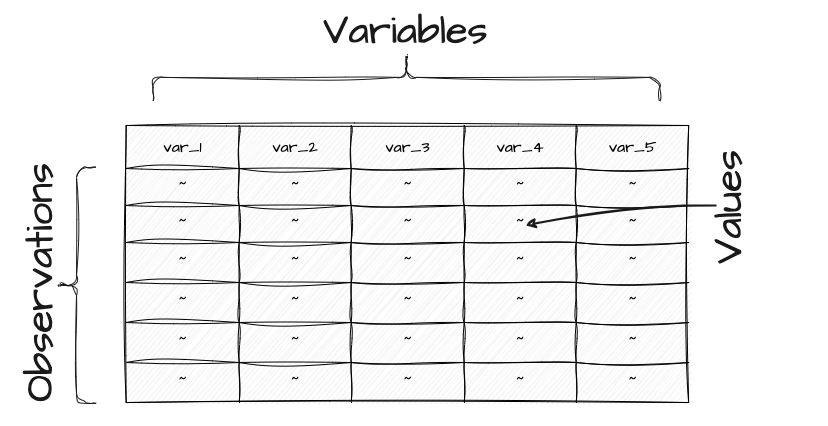
\includegraphics[width=2.76in,height=\textheight]{figures/understanding-data/ud-tidy.drawio.png}

}

\caption{\label{fig-ud-tidy-format-image}Visual summary of the tidy
format.}

\end{figure}

In terms of semantics, columns and rows both contribute to the
informational value of the dataset. Let's start with columns. In a tidy
dataset, each column is a variable, an attribute that can take on a
number of values. Although variables vary in terms of values, they do
not in type. A variable is of one and only one informational type.
Statistically speaking, informational types are defined as
\textbf{levels of measurement}, a classification system used to
semantically distiguish between types of variables. There are four
levels (or types) in this system: nominal, ordinal, interval, and ratio.

In practice, however, text analysis researchers often group these levels
into three main informational types: categorical, ordinal, and numeric
(\protect\hyperlink{ref-Gries2021a}{S. T. Gries 2021}). What do these
informational types represent? \textbf{Categorical data} is for labeled
data or classes that answer the question ``what?'' \textbf{Ordinal data}
is categorical data with rank order that answers the question ``what
order?'' \textbf{Numeric data} is ordinal data with equal intervals
between values that answers the question ``how much or how many?''

Let's look at an example of a tidy dataset. Using the criteria just
described, let's see if we can identify the informational values
(categorical, ordinal, or numeric) of the variables that appear in a
snippet from the MASC corpus in dataset form in
Table~\ref{tbl-ud-info-values-masc}.

\hypertarget{tbl-ud-info-values-masc}{}
\begin{longtable}[]{@{}
  >{\raggedright\arraybackslash}p{(\columnwidth - 12\tabcolsep) * \real{0.2576}}
  >{\raggedright\arraybackslash}p{(\columnwidth - 12\tabcolsep) * \real{0.1364}}
  >{\raggedleft\arraybackslash}p{(\columnwidth - 12\tabcolsep) * \real{0.0758}}
  >{\raggedleft\arraybackslash}p{(\columnwidth - 12\tabcolsep) * \real{0.1212}}
  >{\raggedright\arraybackslash}p{(\columnwidth - 12\tabcolsep) * \real{0.1667}}
  >{\raggedright\arraybackslash}p{(\columnwidth - 12\tabcolsep) * \real{0.0606}}
  >{\raggedleft\arraybackslash}p{(\columnwidth - 12\tabcolsep) * \real{0.1818}}@{}}
\caption{\label{tbl-ud-info-values-masc}MASC dataset
variables.}\tabularnewline
\toprule\noalign{}
\begin{minipage}[b]{\linewidth}\raggedright
title
\end{minipage} & \begin{minipage}[b]{\linewidth}\raggedright
modality
\end{minipage} & \begin{minipage}[b]{\linewidth}\raggedleft
date
\end{minipage} & \begin{minipage}[b]{\linewidth}\raggedleft
ref\_num
\end{minipage} & \begin{minipage}[b]{\linewidth}\raggedright
word
\end{minipage} & \begin{minipage}[b]{\linewidth}\raggedright
pos
\end{minipage} & \begin{minipage}[b]{\linewidth}\raggedleft
num\_letters
\end{minipage} \\
\midrule\noalign{}
\endfirsthead
\toprule\noalign{}
\begin{minipage}[b]{\linewidth}\raggedright
title
\end{minipage} & \begin{minipage}[b]{\linewidth}\raggedright
modality
\end{minipage} & \begin{minipage}[b]{\linewidth}\raggedleft
date
\end{minipage} & \begin{minipage}[b]{\linewidth}\raggedleft
ref\_num
\end{minipage} & \begin{minipage}[b]{\linewidth}\raggedright
word
\end{minipage} & \begin{minipage}[b]{\linewidth}\raggedright
pos
\end{minipage} & \begin{minipage}[b]{\linewidth}\raggedleft
num\_letters
\end{minipage} \\
\midrule\noalign{}
\endhead
\bottomrule\noalign{}
\endlastfoot
Hotel California & Writing & 2008 & 0 & \textgreater{} & NN & 1 \\
Hotel California & Writing & 2008 & 1 & Hotel & NNP & 5 \\
Hotel California & Writing & 2008 & 2 & California & NNP & 10 \\
Hotel California & Writing & 2008 & 3 & Fact & NNP & 4 \\
Hotel California & Writing & 2008 & 4 & : & : & 1 \\
Hotel California & Writing & 2008 & 5 & Sound & NNP & 5 \\
Hotel California & Writing & 2008 & 6 & is & VBZ & 2 \\
Hotel California & Writing & 2008 & 7 & a & DT & 1 \\
Hotel California & Writing & 2008 & 8 & vibration & NN & 9 \\
Hotel California & Writing & 2008 & 9 & . & . & 1 \\
\end{longtable}

We have seven variables listed as headers for each of the columns. We
could go one-by-one left-to-right but let's take another tack. Instead,
let's identify all those variables that cannot be numeric --these are
all the non-numeral variables: \texttt{title}, \texttt{modality},
\texttt{word}, and \texttt{pos}. The question to ask of these variables
is whether they represent an order or rank. Since titles, modalities,
words, and parts-of-speech are not ordered values, they are all
categorical.

Now in relation to \texttt{date}, \texttt{ref\_num}, and
\texttt{num\_letters}. All three are numerals, so they could be numeric.
But they could also be numeral representations of ordinal data. Before
we can move forward, we need to make sure we understand what each
variable means and how it is measured, or \textbf{operationalized}. The
variable name and the values can be helpful in this respect.
\texttt{date} is what it sounds like, a date, and is operationalized as
a year in the Gregorian calendar. And \texttt{num\_letters} seems quite
descriptive as well, number of letters, appearing as a letter count. But
in some cases it may be opaque as to what is being measured by the
variable name alone, for example \texttt{ref\_num}, and one will have to
refer to the dataset documentation. In this case \texttt{ref\_num} is a
reference number operationalized as a unique identifier for each word
per document in the corpus.

With this in mind, let's return to the question of whether
\texttt{date}, \texttt{ref\_num}, and \texttt{num\_letters} are numeric
or ordinal. Starting with the trickiest one, \texttt{date}, we can ask
the question to identify numeric data: ``how much or how many?''. In the
case of \texttt{date}, the answer is neither. A date is a point in time,
not a quantity. So \texttt{date} is not numeric. But it does provide
information about order. Hence, \texttt{date} is ordinal.
\texttt{ref\_num} is also ordinal because the question ``what order?''
can be asked of it. Finally, \texttt{num\_letters} is numeric because it
answers the question ``how many?''.

Let's turn to the second semantic value of a tidy dataset. In a tidy
dataset, each row is an observation. But an observation of what? This
depends on what the unit of observation is. That sounds circular, but
its not. The \textbf{unit of observation} is simply the primary entity
that is being observed. Without context, it can it can be identified in
a dataset by looking at the level of specificity of the variable values
and asking what each variable describes. When one variable appears to be
the most individualized and other variables appear to describe that
variable, then the most individualized variable is likely the unit of
observation of the dataset, \emph{i.e.} the meaning of each observation.

Applying these strategies to the Table in \ref{tbl-ud-info-values-masc},
we can see that each observation at its core is a word. We see that the
values of each observation are the attributes of each word.
\texttt{word} is the most individualized variable and the \texttt{pos}
(part-of-speech), \texttt{num\_letters}, and \texttt{ref\_num} all
describe the word.

The other variables \texttt{title}, \texttt{modality}, and \texttt{date}
are not direct attributes of the word. Instead, they are attributes of
the document in which the word appears. Together, however, they all
provide information about the word.

\begin{tcolorbox}[enhanced jigsaw, rightrule=.15mm, leftrule=.75mm, opacityback=0, arc=.35mm, colback=white, breakable, toprule=.15mm, bottomrule=.15mm, left=2mm]

\textbf{\faIcon{lightbulb} Consider this}

Data can be organized in many ways. It is important to make clear that
data in tabular format in itself does not constitute a dataset, in the
tidy sense we will be using. Can you think of examples of tabular
information that would not be in a tidy format? What would be the
implications of this for data analysis?

\end{tcolorbox}

As we round out this section on data organization, it is important to
stress that the purpose of curation is to represent the corpus data in
an informative, tidy format. A curated dataset serves as a reference
point making relationships explicit, enabling more efficient querying,
and paving the way for further processing before analysis. In the
subsequent section, we will highlight common approaches to modifying the
curated dataset, either row-wise or column-wise, to make it more
amenable to the particular aims of a given analysis.

\hypertarget{sec-ud-transformation}{%
\subsection{Transformation}\label{sec-ud-transformation}}

At this point have introduced the first step creating a dataset ready
for analysis, data curation. However, a curated dataset is rarely the
final organizational step before proceeding to statistical analysis.
Many times, if not always, the curated dataset requires \textbf{data
transformation} to derive or generate new data for the dataset. This
process may incur row-wise (observation) or column-wise (variable) level
changes, as illustrated in Figure~\ref{fig-ud-transformations}.

\begin{figure}[H]

{\centering 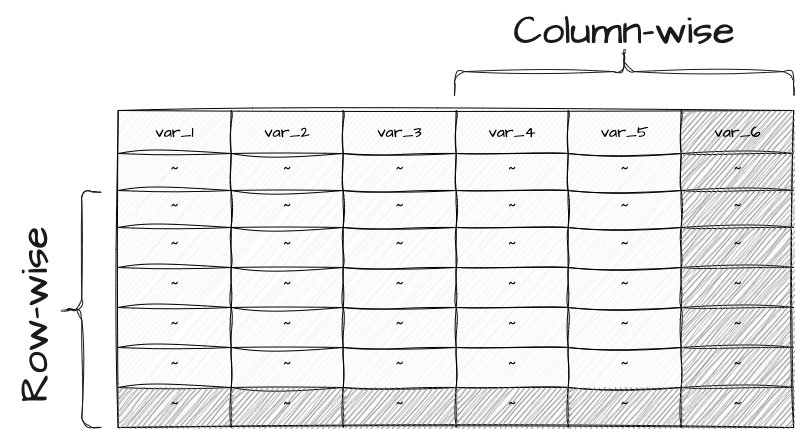
\includegraphics[width=2.65in,height=\textheight]{figures/understanding-data/ud-transformations.drawio.png}

}

\caption{\label{fig-ud-transformations}Visualization of row-wise and
column-wise transformation operations on a dataset.}

\end{figure}

The results build on and manipulate the curated dataset to produce a
\emph{derived dataset}. While there is typically one curated dataset
that serves as the base organizational dataset, there may be multiple
derived datasets, each aligning with the informational needs of specific
analyses in the research project.

In what follows, we will discuss the most common types of data
transformation: text normalization, text tokenization, variable
recoding, variable generation, and observation/ variable merging. Note,
however, that the order in which these transformations are applied in a
given research project is not fixed and will vary depending on the
dataset and the research question(s) to be addressed.

\hypertarget{sec-ud-text-normalization}{%
\subsubsection{Text normalization}\label{sec-ud-text-normalization}}

The process of text normalization aims to prepare and standardize text.
It is often a preliminary step in data transformation processes which
include variables with text. The aim is to convert the text into a
uniform format to reduce unwanted variation and noise.

Let's take a toy dataset, in Table~\ref{tbl-ud-text-dataset}, as an
example starting point. In this dataset, we have two variables,
\texttt{text\_id} and \texttt{text}. It only has one observation.

\hypertarget{tbl-ud-text-dataset}{}
\begin{longtable}[]{@{}
  >{\raggedright\arraybackslash}p{(\columnwidth - 2\tabcolsep) * \real{0.1000}}
  >{\raggedright\arraybackslash}p{(\columnwidth - 2\tabcolsep) * \real{0.9000}}@{}}
\caption{\label{tbl-ud-text-dataset}A toy dataset with two variables,
\texttt{text\_id} and \texttt{text}.}\tabularnewline
\toprule\noalign{}
\begin{minipage}[b]{\linewidth}\raggedright
text\_id
\end{minipage} & \begin{minipage}[b]{\linewidth}\raggedright
text
\end{minipage} \\
\midrule\noalign{}
\endfirsthead
\toprule\noalign{}
\begin{minipage}[b]{\linewidth}\raggedright
text\_id
\end{minipage} & \begin{minipage}[b]{\linewidth}\raggedright
text
\end{minipage} \\
\midrule\noalign{}
\endhead
\bottomrule\noalign{}
\endlastfoot
1 & It's a beautiful day in the US, and our group decided to visit the
famous Grand Canyon. As we reached the destination, Jane said, ``I can't
believe we're finally here!'' The breathtaking view left us speechless;
indeed, it was a sight to behold. During our trip, we encountered
tourists from different countries, sharing stories and laughter. For all
of us, this experience will be cherished forever. \\
\end{longtable}

The types of transformations we apply will depend on the specific needs
of the project, but can include those found in
Table~\ref{tbl-ud-text-normalization}.

\hypertarget{tbl-ud-text-normalization}{}
\begin{longtable}[]{@{}
  >{\raggedright\arraybackslash}p{(\columnwidth - 4\tabcolsep) * \real{0.2500}}
  >{\raggedright\arraybackslash}p{(\columnwidth - 4\tabcolsep) * \real{0.3000}}
  >{\raggedright\arraybackslash}p{(\columnwidth - 4\tabcolsep) * \real{0.4500}}@{}}
\caption{\label{tbl-ud-text-normalization}Common text normalization
tasks}\tabularnewline
\toprule\noalign{}
\begin{minipage}[b]{\linewidth}\raggedright
Task name
\end{minipage} & \begin{minipage}[b]{\linewidth}\raggedright
Relevant example
\end{minipage} & \begin{minipage}[b]{\linewidth}\raggedright
Typical purpose
\end{minipage} \\
\midrule\noalign{}
\endfirsthead
\toprule\noalign{}
\begin{minipage}[b]{\linewidth}\raggedright
Task name
\end{minipage} & \begin{minipage}[b]{\linewidth}\raggedright
Relevant example
\end{minipage} & \begin{minipage}[b]{\linewidth}\raggedright
Typical purpose
\end{minipage} \\
\midrule\noalign{}
\endhead
\bottomrule\noalign{}
\endlastfoot
Lowercasing & \texttt{"Text"} to \texttt{"text"} & Minimizing case
sensitivity in subsequent analysis \\
Removal of Punctuation and Special Characters &
\texttt{"Hello,\ World!"} to \texttt{"Hello\ World"} & Removing
non-alphanumeric characters that may not carry semantic value \\
Adjustment of Forms & \texttt{"colour"} to \texttt{"color"},
\texttt{"it\textquotesingle{}s"} to \texttt{"it\ is"}, \texttt{"1"} to
\texttt{"one"} & Standardizing variations in spelling, contractions, and
numeric forms to a common format \\
Stopword Removal & \texttt{"This\ is\ a\ sentence"} to
\texttt{"This\ sentence"} & Discarding common words that usually do not
contain meaningful semantic information \\
\end{longtable}

These transformations are column-wise operations, meaning they preserve
the number of rows in the dataset. They also preserve the number of
columns, but \emph{do} change the values of the variables. These tasks
should be applied with an understanding of how the changes will impact
the analysis. For example, lowercasing can be useful for reducing
differences between words that are otherwise identical, yet differ in
case due to word position in a sentence (``The'' versus ``the'').
However, lowercasing can also be problematic if the case of the word
carries semantic value, such as in the case of ``US'' (United States)
and ``us'' (first person plural pronoun). The same can be said for
removing or adjusting particular characters and discarding stopwords.

\begin{tcolorbox}[enhanced jigsaw, rightrule=.15mm, leftrule=.75mm, opacityback=0, arc=.35mm, colback=white, breakable, toprule=.15mm, bottomrule=.15mm, left=2mm]

\textbf{\faIcon{medal} Dive deeper}

Stopwords are words that are so commonly used in a language that they
tend not to contribute much to the meaning of a sentence. There are
various predefined lists of stopwords for different languages available
on the web and through R in the \texttt{stopwords} package
(\protect\hyperlink{ref-R-stopwords}{Benoit, Muhr, and Watanabe 2021}).
However, it is important to note the criteria used to determine which
words are considered stopwords in a particular resource may not fit a
researcher's needs or the characteristics of the data. Learn more about
stopwords in Kaur and Buttar (\protect\hyperlink{ref-Kaur2018}{2018}).

\end{tcolorbox}

Let's be conservative and only apply lowercasing to our toy dataset as
seen in Table~\ref{tbl-ud-text-dataset-lowercase}.

\hypertarget{tbl-ud-text-dataset-lowercase}{}
\begin{longtable}[]{@{}
  >{\raggedright\arraybackslash}p{(\columnwidth - 2\tabcolsep) * \real{0.1000}}
  >{\raggedright\arraybackslash}p{(\columnwidth - 2\tabcolsep) * \real{0.9000}}@{}}
\caption{\label{tbl-ud-text-dataset-lowercase}A toy dataset with two
variables, \texttt{text\_id} and \texttt{text}, where the text has been
lowercased.}\tabularnewline
\toprule\noalign{}
\begin{minipage}[b]{\linewidth}\raggedright
text\_id
\end{minipage} & \begin{minipage}[b]{\linewidth}\raggedright
text
\end{minipage} \\
\midrule\noalign{}
\endfirsthead
\toprule\noalign{}
\begin{minipage}[b]{\linewidth}\raggedright
text\_id
\end{minipage} & \begin{minipage}[b]{\linewidth}\raggedright
text
\end{minipage} \\
\midrule\noalign{}
\endhead
\bottomrule\noalign{}
\endlastfoot
1 & it's a beautiful day in the us, and our group decided to visit the
famous grand canyon. as we reached the destination, jane said, ``i can't
believe we're finally here!'' the breathtaking view left us speechless;
indeed, it was a sight to behold. during our trip, we encountered
tourists from different countries, sharing stories and laughter. for all
of us, this experience will be cherished forever. \\
\end{longtable}

When text normalization steps are motivated and applied with foresight
they serve to enhance the quality of the data and improves the
reliability of subsequent transformation steps.

\hypertarget{sec-ud-text-tokenization}{%
\subsubsection{Text tokenization}\label{sec-ud-text-tokenization}}

Another text-oriented transformation step is \textbf{text tokenization}.
This process involves adapting the text such that it reflects the target
linguistic unit that will be used in the analysis. This is a row-wise
operation expanding the number of rows, if the linguistic unit is
smaller than the original variable, or reducing the number of rows, if
the linguistic unit is larger than the original variable. At its core,
tokenization is the process which enables the quantitative analysis of
text.

Text variables can be tokenized at any linguistic level. To illustrate,
consider our toy dataset from Table~\ref{tbl-ud-text-dataset-lowercase}.
We can tokenize the text at the sentence level, in
Table~\ref{tbl-ud-text-dataset-tokenization-sentence}, by splitting the
text at the period followed by a space. This results in a dataset with
four observations, one for each sentence in the original text.

\hypertarget{tbl-ud-text-dataset-tokenization-sentence}{}
\begin{longtable}[]{@{}
  >{\raggedright\arraybackslash}p{(\columnwidth - 2\tabcolsep) * \real{0.1000}}
  >{\raggedright\arraybackslash}p{(\columnwidth - 2\tabcolsep) * \real{0.9000}}@{}}
\caption{\label{tbl-ud-text-dataset-tokenization-sentence}A toy dataset
with two variables, \texttt{text\_id} and \texttt{sentence}, where the
text has been tokenized at the sentence level.}\tabularnewline
\toprule\noalign{}
\begin{minipage}[b]{\linewidth}\raggedright
text\_id
\end{minipage} & \begin{minipage}[b]{\linewidth}\raggedright
sentence
\end{minipage} \\
\midrule\noalign{}
\endfirsthead
\toprule\noalign{}
\begin{minipage}[b]{\linewidth}\raggedright
text\_id
\end{minipage} & \begin{minipage}[b]{\linewidth}\raggedright
sentence
\end{minipage} \\
\midrule\noalign{}
\endhead
\bottomrule\noalign{}
\endlastfoot
1 & it's a beautiful day in the us, and our group decided to visit the
famous grand canyon \\
1 & as we reached the destination, jane said, ``i can't believe we're
finally here!'' the breathtaking view left us speechless; indeed, it was
a sight to behold \\
1 & during our trip, we encountered tourists from different countries,
sharing stories and laughter \\
1 & for all of us, this experience will be cherished forever. \\
\end{longtable}

It is important to make explicit what the operationalization of our
linguistic unit is as common terms such as sentence, word, \emph{etc.}
can be defined in different ways. For example, the sentence tokenization
above is based on the assumption that sentences are separated by a
period followed by a space. This is a suitable definition for this text,
but likely will not be for other English text or for other languages/
writing scripts. For words, a very simple operationalization is to use
whitespace separation (\emph{e.g.} ``I cannot believe it.'' -- {[}``I'',
``cannot'', ``believe'', ``it.''{]}). However, this approach does not
handle puntuation marks (\emph{e.g.} {[}``it.''{]}) or contractions
(\emph{e.g.} {[}``can't''{]}). A more sophisticated operationalization
will be necessary for these, and possibly other, cases.

Another important token unit is the \(n\)-gram. Words or characters can
be grouped into contiguous sequences with a moving window of a certain
size \(n\). Single unit windows are referred to as unigrams, two units
as bigrams, three units as trigrams, and so on. Let's tokenize our toy
dataset at the bigram level for words using a simple whitespace
separation for words, as seen in Table~\ref{tbl-ud-text-dataset-bigram}.

\hypertarget{tbl-ud-text-dataset-bigram}{}
\begin{longtable}[]{@{}ll@{}}
\caption{\label{tbl-ud-text-dataset-bigram}A toy dataset with two
variables, \texttt{text\_id} and \texttt{bigram}, where the text has
been tokenized at the bigram word level.}\tabularnewline
\toprule\noalign{}
text\_id & word \\
\midrule\noalign{}
\endfirsthead
\toprule\noalign{}
text\_id & word \\
\midrule\noalign{}
\endhead
\bottomrule\noalign{}
\endlastfoot
1 & it's a \\
1 & a beautiful \\
1 & beautiful day \\
1 & day in \\
1 & in the \\
1 & the us \\
1 & us and \\
1 & and our \\
1 & our group \\
1 & group decided \\
\end{longtable}

In Table~\ref{tbl-ud-text-dataset-bigram} we see that the first bigram
is ``it's a'' --the first two words (based on whitespace separation) in
the text. The second bigram is ``a toy'' --the second and third words in
the text. This continues to the end of the text. \(N\)-gram tokenization
can be useful to capture context that would otherwise would be lost from
tokenizing words or characters at the unigram level.

Up to this point our tokens have been surface forms. That is, they are
the actual words or characters as they appear in the text. However, we
may want to reduce the tokens to their base form, removing their
inflectional forms. This is known as \textbf{lemmatization}. For
example, the word ``run'' is the lemma of the words ``running'',
``runs'', and ``ran''. Let's lemmatize the third sentence in our toy
dataset. For comparison, \texttt{word} and \texttt{lemma} are shown
side-by-side in Table~\ref{tbl-ud-text-dataset-lemmatization}.

\hypertarget{tbl-ud-text-dataset-lemmatization}{}
\begin{longtable}[]{@{}lll@{}}
\caption{\label{tbl-ud-text-dataset-lemmatization}A toy dataset with two
variables, \texttt{text\_id} and \texttt{word}, where the text has been
tokenized at the unigram word level and lemmatized.}\tabularnewline
\toprule\noalign{}
text\_id & word & lemma \\
\midrule\noalign{}
\endfirsthead
\toprule\noalign{}
text\_id & word & lemma \\
\midrule\noalign{}
\endhead
\bottomrule\noalign{}
\endlastfoot
1 & during & during \\
1 & our & our \\
1 & trip & trip \\
1 & we & we \\
1 & encountered & encounter \\
1 & tourists & tourist \\
1 & from & from \\
1 & different & different \\
1 & countries & country \\
1 & sharing & share \\
1 & stories & story \\
1 & and & and \\
1 & laughter & laughter \\
\end{longtable}

\begin{tcolorbox}[enhanced jigsaw, rightrule=.15mm, leftrule=.75mm, opacityback=0, arc=.35mm, colback=white, breakable, toprule=.15mm, bottomrule=.15mm, left=2mm]

\textbf{\faIcon{file-alt} Case study}

Inflectional family size is the number of inflectional forms for a given
word and can be calculated from a corpus by counting the number of
surface forms for each lemma in the corpus
(\protect\hyperlink{ref-Kostic2003}{Kostić, Marković, and Baucal 2003}).
Baayen, Feldman, and Schreuder
(\protect\hyperlink{ref-Baayen2006}{2006}) found that words with larger
inflectional family size are associated with faster word recognition
times in lexical processing tasks.

\end{tcolorbox}

Together tokenization and lemmatization are powerful tools for
transforming text. If our dataset contains more robust linguistic
annotation or that annotation can be generated (see
Section~\ref{sec-ud-variable-generation}), this information can also be
leveraged to tokenize language into a format that is easier to explore
and quantify in an analysis.

\hypertarget{sec-ud-variable-recoding}{%
\subsubsection{Variable recoding}\label{sec-ud-variable-recoding}}

Recoding is the process of transforming the values of one or more
variables into new values which are more amenable to analysis. The aim
is to simplify complex variables, making it easier to identify patterns
and trends relevant for the research question. This is a column-wise
operation which can be applied to categorical or numeric variables.

Let's return to the MASC dataset and demonstrate recoding of categorical
and numeric variables. In Table~\ref{tbl-ud-info-values-masc} the
\texttt{pos} variable whose values represent the part-of-speech (POS) of
each token in the text. The measure is a POS tag from the Penn Treebank
tagset (\protect\hyperlink{ref-Marcus1993}{Marcus, Santorini, and
Marcinkiewicz 1993}). This tagset makes twelve major and 45 minor
grammatical class distinctions. In an analysis that aims to explore only
major class distinctions, it would be useful to recode the \texttt{pos}
variable into major classes only (\emph{i.e.} noun, pronoun, adjective,
verb, adverb, \emph{etc.}) to facilitate queries, summaries, and
visualizations.

\hypertarget{tbl-ud-recode-categorical}{}
\begin{longtable}[]{@{}
  >{\raggedright\arraybackslash}p{(\columnwidth - 14\tabcolsep) * \real{0.2179}}
  >{\raggedright\arraybackslash}p{(\columnwidth - 14\tabcolsep) * \real{0.1154}}
  >{\raggedleft\arraybackslash}p{(\columnwidth - 14\tabcolsep) * \real{0.0641}}
  >{\raggedleft\arraybackslash}p{(\columnwidth - 14\tabcolsep) * \real{0.1026}}
  >{\raggedright\arraybackslash}p{(\columnwidth - 14\tabcolsep) * \real{0.1410}}
  >{\raggedright\arraybackslash}p{(\columnwidth - 14\tabcolsep) * \real{0.0513}}
  >{\raggedright\arraybackslash}p{(\columnwidth - 14\tabcolsep) * \real{0.1538}}
  >{\raggedleft\arraybackslash}p{(\columnwidth - 14\tabcolsep) * \real{0.1538}}@{}}
\caption{\label{tbl-ud-recode-categorical}A toy dataset with three
variables, \texttt{text\_id}, \texttt{pos}, \texttt{major\_pos}, where
the \texttt{pos} variable has been recoded into major grammatical
classes \texttt{major\_pos}.}\tabularnewline
\toprule\noalign{}
\begin{minipage}[b]{\linewidth}\raggedright
title
\end{minipage} & \begin{minipage}[b]{\linewidth}\raggedright
modality
\end{minipage} & \begin{minipage}[b]{\linewidth}\raggedleft
date
\end{minipage} & \begin{minipage}[b]{\linewidth}\raggedleft
ref\_num
\end{minipage} & \begin{minipage}[b]{\linewidth}\raggedright
word
\end{minipage} & \begin{minipage}[b]{\linewidth}\raggedright
pos
\end{minipage} & \begin{minipage}[b]{\linewidth}\raggedright
major\_pos
\end{minipage} & \begin{minipage}[b]{\linewidth}\raggedleft
num\_letters
\end{minipage} \\
\midrule\noalign{}
\endfirsthead
\toprule\noalign{}
\begin{minipage}[b]{\linewidth}\raggedright
title
\end{minipage} & \begin{minipage}[b]{\linewidth}\raggedright
modality
\end{minipage} & \begin{minipage}[b]{\linewidth}\raggedleft
date
\end{minipage} & \begin{minipage}[b]{\linewidth}\raggedleft
ref\_num
\end{minipage} & \begin{minipage}[b]{\linewidth}\raggedright
word
\end{minipage} & \begin{minipage}[b]{\linewidth}\raggedright
pos
\end{minipage} & \begin{minipage}[b]{\linewidth}\raggedright
major\_pos
\end{minipage} & \begin{minipage}[b]{\linewidth}\raggedleft
num\_letters
\end{minipage} \\
\midrule\noalign{}
\endhead
\bottomrule\noalign{}
\endlastfoot
Hotel California & Writing & 2008 & 0 & \textgreater{} & NN & noun &
1 \\
Hotel California & Writing & 2008 & 1 & Hotel & NNP & noun & 5 \\
Hotel California & Writing & 2008 & 2 & California & NNP & noun & 10 \\
Hotel California & Writing & 2008 & 3 & Fact & NNP & noun & 4 \\
Hotel California & Writing & 2008 & 4 & : & : & punctuation & 1 \\
Hotel California & Writing & 2008 & 5 & Sound & NNP & noun & 5 \\
Hotel California & Writing & 2008 & 6 & is & VBZ & verb & 2 \\
Hotel California & Writing & 2008 & 7 & a & DT & determiner & 1 \\
Hotel California & Writing & 2008 & 8 & vibration & NN & noun & 9 \\
Hotel California & Writing & 2008 & 9 & . & . & punctuation & 1 \\
\end{longtable}

In Table~\ref{tbl-ud-recode-categorical}, the \texttt{pos} variable has
been recoded into major grammatical classes. The \texttt{major\_pos}
variable is a categorical variable with 12 levels, one for each major
grammatical class in the Penn Treebank tagset. While the demonstration
here demonstrates the simplification of a categorical variable, recoding
can also be used to transliterate categorical variables. Continuing with
the theme of POS tags, the \texttt{pos} variable could be recoded into a
different tagset, such as the Universal Dependencies tagset
(\protect\hyperlink{ref-Nivre2016}{Nivre et al. 2016}).

Now, let's look at recoding the numeric variable \texttt{num\_letters}.
This variable represents the number of letters in each token. In the
MASC dataset, the \texttt{num\_letters} variable is a numeric variable
with a range of values from 1 to 21. In some analyses, it may be useful
to recode this variable into discrete categories, or bins, such as
short, medium, and long words.

\hypertarget{tbl-ud-recode-numeric}{}
\begin{longtable}[]{@{}
  >{\raggedright\arraybackslash}p{(\columnwidth - 16\tabcolsep) * \real{0.1889}}
  >{\raggedright\arraybackslash}p{(\columnwidth - 16\tabcolsep) * \real{0.1000}}
  >{\raggedleft\arraybackslash}p{(\columnwidth - 16\tabcolsep) * \real{0.0556}}
  >{\raggedleft\arraybackslash}p{(\columnwidth - 16\tabcolsep) * \real{0.0889}}
  >{\raggedright\arraybackslash}p{(\columnwidth - 16\tabcolsep) * \real{0.1222}}
  >{\raggedright\arraybackslash}p{(\columnwidth - 16\tabcolsep) * \real{0.0444}}
  >{\raggedright\arraybackslash}p{(\columnwidth - 16\tabcolsep) * \real{0.1333}}
  >{\raggedleft\arraybackslash}p{(\columnwidth - 16\tabcolsep) * \real{0.1333}}
  >{\raggedright\arraybackslash}p{(\columnwidth - 16\tabcolsep) * \real{0.1333}}@{}}
\caption{\label{tbl-ud-recode-numeric}The MASC dataset with the
\texttt{num\_letters} variable recoded into three categories: short,
medium, and long words in \texttt{word\_length}.}\tabularnewline
\toprule\noalign{}
\begin{minipage}[b]{\linewidth}\raggedright
title
\end{minipage} & \begin{minipage}[b]{\linewidth}\raggedright
modality
\end{minipage} & \begin{minipage}[b]{\linewidth}\raggedleft
date
\end{minipage} & \begin{minipage}[b]{\linewidth}\raggedleft
ref\_num
\end{minipage} & \begin{minipage}[b]{\linewidth}\raggedright
word
\end{minipage} & \begin{minipage}[b]{\linewidth}\raggedright
pos
\end{minipage} & \begin{minipage}[b]{\linewidth}\raggedright
major\_pos
\end{minipage} & \begin{minipage}[b]{\linewidth}\raggedleft
num\_letters
\end{minipage} & \begin{minipage}[b]{\linewidth}\raggedright
word\_length
\end{minipage} \\
\midrule\noalign{}
\endfirsthead
\toprule\noalign{}
\begin{minipage}[b]{\linewidth}\raggedright
title
\end{minipage} & \begin{minipage}[b]{\linewidth}\raggedright
modality
\end{minipage} & \begin{minipage}[b]{\linewidth}\raggedleft
date
\end{minipage} & \begin{minipage}[b]{\linewidth}\raggedleft
ref\_num
\end{minipage} & \begin{minipage}[b]{\linewidth}\raggedright
word
\end{minipage} & \begin{minipage}[b]{\linewidth}\raggedright
pos
\end{minipage} & \begin{minipage}[b]{\linewidth}\raggedright
major\_pos
\end{minipage} & \begin{minipage}[b]{\linewidth}\raggedleft
num\_letters
\end{minipage} & \begin{minipage}[b]{\linewidth}\raggedright
word\_length
\end{minipage} \\
\midrule\noalign{}
\endhead
\bottomrule\noalign{}
\endlastfoot
Hotel California & Writing & 2008 & 0 & \textgreater{} & NN & noun & 1 &
short \\
Hotel California & Writing & 2008 & 1 & Hotel & NNP & noun & 5 &
medium \\
Hotel California & Writing & 2008 & 2 & California & NNP & noun & 10 &
long \\
Hotel California & Writing & 2008 & 3 & Fact & NNP & noun & 4 &
medium \\
Hotel California & Writing & 2008 & 4 & : & : & punctuation & 1 &
short \\
Hotel California & Writing & 2008 & 5 & Sound & NNP & noun & 5 &
medium \\
Hotel California & Writing & 2008 & 6 & is & VBZ & verb & 2 & short \\
Hotel California & Writing & 2008 & 7 & a & DT & determiner & 1 &
short \\
Hotel California & Writing & 2008 & 8 & vibration & NN & noun & 9 &
long \\
Hotel California & Writing & 2008 & 9 & . & . & punctuation & 1 &
short \\
\end{longtable}

In Table~\ref{tbl-ud-recode-numeric} the variable \texttt{word\_length}
appears with the values \texttt{short}, \texttt{medium}, and
\texttt{long}. This is now a categorical variable of type ordinal. Of
note, is that the operational definition of used to create these word
length bins should be made explicit in the documentation of the dataset.

In sum, recoding is a useful data transformation technique that can be
used to simplify complex variables, making it easier to identify
patterns and trends relevant for the research question.

\hypertarget{sec-ud-variable-generation}{%
\subsubsection{Variable generation}\label{sec-ud-variable-generation}}

The process of variable generation aims to augment existing variables or
create new ones, and as such is a column-wise operation. Generation can
include applying calculations or extracting relevant information from
existing variables or enhancing text variables with linguistic
annotation. Simplifying a bit, generation helps make implicit attributes
explicit. The results of this process enables direct access during
analysis to features that were otherwise hidden or difficult to access.

Let's highlight a some common calculation and extraction examples that
generate variables. First, let's look at the calculation of measures. In
text analysis, measures are often used to describe the properties of a
document or linguistic unit. For example, the number of words in a
corpus document, the lengths of sentences, the number of clauses in a
sentence, \emph{etc.}. In turn, these measures can be used to calculate
other measures, such as lexical diversity or syntactic complexity
measures.

In terms of extraction, the goal is to distill relevant information from
existing variables. For example, extracting the year from a date
variable, or extracting the first name from a full name variable. In
text analysis, extraction is often used to extract information from text
variables. Say we have a dataset with a variable containing conversation
utterances. We may want to extract some characteristic from those
utterances and capture their occurrence in a new variable.

But what if we want to extract linguistic information from a text
variable that is not explicitly present in the text? This is where
linguistic annotation comes in. Linguistic annotation is the process of
enriching text with linguistic information, such as morphological
features, part-of-speech tags, syntactic structure, \emph{etc.}. This
can be done manually by linguist coders and/ or done using natural
language processing (NLP) tools, many of which are available in R (see
Chapter~\ref{sec-transform-datasets}).

To illustrate the process of generating linguistic annotation with
existing tools, I will use the plain text version of the MASC. In
Table~\ref{tbl-ud-masc-plain-dataset}, the text has been organized into
a dataset and tokenized into sentences. The \texttt{text\_id} variable
is a unique identifier for each document, and the \texttt{sentence\_id}
variable is a unique identifier for each sentence.

\hypertarget{tbl-ud-masc-plain-dataset}{}
\begin{longtable}[]{@{}
  >{\raggedright\arraybackslash}p{(\columnwidth - 4\tabcolsep) * \real{0.1500}}
  >{\raggedleft\arraybackslash}p{(\columnwidth - 4\tabcolsep) * \real{0.1500}}
  >{\raggedright\arraybackslash}p{(\columnwidth - 4\tabcolsep) * \real{0.7000}}@{}}
\caption{\label{tbl-ud-masc-plain-dataset}A MASC sample document in
dataset tokenized into sentences.}\tabularnewline
\toprule\noalign{}
\begin{minipage}[b]{\linewidth}\raggedright
text\_id
\end{minipage} & \begin{minipage}[b]{\linewidth}\raggedleft
sentence\_id
\end{minipage} & \begin{minipage}[b]{\linewidth}\raggedright
sentence
\end{minipage} \\
\midrule\noalign{}
\endfirsthead
\toprule\noalign{}
\begin{minipage}[b]{\linewidth}\raggedright
text\_id
\end{minipage} & \begin{minipage}[b]{\linewidth}\raggedleft
sentence\_id
\end{minipage} & \begin{minipage}[b]{\linewidth}\raggedright
sentence
\end{minipage} \\
\midrule\noalign{}
\endhead
\bottomrule\noalign{}
\endlastfoot
1 & 1 & \textgreater Hotel California Fact: Sound is a vibration. \\
1 & 2 & Sound travels as a mechanical wave through a medium, and in
space, there is no medium. \\
1 & 3 & So when my shuttle malfunctioned and the airlocks didn't keep
the air in, I heard nothing. \\
1 & 4 & After the first whoosh of the air being sucked away, there was
lightning, but no thunder. \\
1 & 5 & Eyes bulging in panic, but no screams. \\
\end{longtable}

Applying a pre-trained model from the
\href{https://universaldependencies.org/}{Universal Dependencies
(UD)}\footnote{The Universal Dependency project is an effort to develop
  cross-linguistically consistent treebank annotation for many
  languages. The project has developed a set of annotation guidelines
  and a set of tools for generating linguistic annotation. The project
  has also developed a set of pre-trained models for many languages.}
project, we can generate linguistic annotation for each token in the
MASC.

\hypertarget{tbl-ud-generate-annotation}{}
\begin{longtable}[]{@{}
  >{\raggedright\arraybackslash}p{(\columnwidth - 12\tabcolsep) * \real{0.0515}}
  >{\raggedleft\arraybackslash}p{(\columnwidth - 12\tabcolsep) * \real{0.0882}}
  >{\raggedright\arraybackslash}p{(\columnwidth - 12\tabcolsep) * \real{0.0662}}
  >{\raggedright\arraybackslash}p{(\columnwidth - 12\tabcolsep) * \real{0.0735}}
  >{\raggedright\arraybackslash}p{(\columnwidth - 12\tabcolsep) * \real{0.0368}}
  >{\raggedright\arraybackslash}p{(\columnwidth - 12\tabcolsep) * \real{0.5441}}
  >{\raggedright\arraybackslash}p{(\columnwidth - 12\tabcolsep) * \real{0.1397}}@{}}
\caption{\label{tbl-ud-generate-annotation}Automatic linguistic
annotation for grammatical category and syntactic structure for an
example English sentence from the MASC.}\tabularnewline
\toprule\noalign{}
\begin{minipage}[b]{\linewidth}\raggedright
doc\_id
\end{minipage} & \begin{minipage}[b]{\linewidth}\raggedleft
sentence\_id
\end{minipage} & \begin{minipage}[b]{\linewidth}\raggedright
token\_id
\end{minipage} & \begin{minipage}[b]{\linewidth}\raggedright
token
\end{minipage} & \begin{minipage}[b]{\linewidth}\raggedright
xpos
\end{minipage} & \begin{minipage}[b]{\linewidth}\raggedright
features
\end{minipage} & \begin{minipage}[b]{\linewidth}\raggedright
syntactic\_relation
\end{minipage} \\
\midrule\noalign{}
\endfirsthead
\toprule\noalign{}
\begin{minipage}[b]{\linewidth}\raggedright
doc\_id
\end{minipage} & \begin{minipage}[b]{\linewidth}\raggedleft
sentence\_id
\end{minipage} & \begin{minipage}[b]{\linewidth}\raggedright
token\_id
\end{minipage} & \begin{minipage}[b]{\linewidth}\raggedright
token
\end{minipage} & \begin{minipage}[b]{\linewidth}\raggedright
xpos
\end{minipage} & \begin{minipage}[b]{\linewidth}\raggedright
features
\end{minipage} & \begin{minipage}[b]{\linewidth}\raggedright
syntactic\_relation
\end{minipage} \\
\midrule\noalign{}
\endhead
\bottomrule\noalign{}
\endlastfoot
1 & 4 & 1 & After & IN & NA & mark \\
1 & 4 & 2 & the & DT & Definite=Def\textbar PronType=Art & det \\
1 & 4 & 3 & first & JJ & Degree=Pos\textbar NumType=Ord & amod \\
1 & 4 & 4 & whoosh & NN & Number=Sing & nsubj:pass \\
1 & 4 & 5 & of & IN & NA & case \\
1 & 4 & 6 & the & DT & Definite=Def\textbar PronType=Art & det \\
1 & 4 & 7 & air & NN & Number=Sing & nmod \\
1 & 4 & 8 & being & VBG & VerbForm=Ger & aux:pass \\
1 & 4 & 9 & sucked & VBN &
Tense=Past\textbar VerbForm=Part\textbar Voice=Pass & advcl \\
1 & 4 & 10 & away & RB & NA & advmod \\
1 & 4 & 11 & , & , & NA & punct \\
1 & 4 & 12 & there & EX & NA & expl \\
1 & 4 & 13 & was & VBD &
Mood=Ind\textbar Number=Sing\textbar Person=3\textbar Tense=Past\textbar VerbForm=Fin
& root \\
1 & 4 & 14 & lightning & NN & Number=Sing & nsubj \\
1 & 4 & 15 & , & , & NA & punct \\
1 & 4 & 16 & but & CC & NA & cc \\
1 & 4 & 17 & no & DT & NA & det \\
1 & 4 & 18 & thunder & NN & Number=Sing & conj \\
1 & 4 & 19 & . & . & NA & punct \\
\end{longtable}

The annotated dataset now includes the key variables \texttt{xpos} (Penn
treebank tags), \texttt{features} (morphological features), and
\texttt{syntactic\_relation}. The results of this process can then be
further transformed as need be to fit the needs of the analysis.

A word of caution: automated linguistic annotation offers rapid access
to abundant and highly dependable linguistic data for numerous
languages. However, linguistic annotation tools are not infallible. They
are tools developed by training computational algorithms to identify
patterns in previously annotated and verified datasets, resulting in a
language model. This model is then employed to predict linguistic
annotations for new language data (as seen in
Table~\ref{tbl-ud-generate-annotation}). The accuracy of the linguistic
annotation heavily relies on the congruence between the language
sampling framework of the trained data and the language data set to be
automatically annotated.

\hypertarget{sec-ud-obs-variable-merging}{%
\subsubsection{Observation/ variable
merging}\label{sec-ud-obs-variable-merging}}

The processing of merging datasets is a transformation step which can be
row-wise or column-wise. Row-wise merging is the process of combining
datasets by appending observations from one dataset to another.
Column-wise merging is the process of combining datasets by appending
variables from one dataset to another. In either case, merging provides
a way to enrich a dataset by incorporating additional information.

To merge in row-wise manner the datasets involved in the process must
have the same variables and variable types. This process is often
referred to as \textbf{concatenating datasets}. It can be thought of as
stacking datasets on top of each other to create a larger dataset.
Remember, having the sample variables and variable types is not the same
has having the same values.

Take, for example, a case when a corpus resource contains data for two
populations. In the course of curating and transforming the datasets it
may make more sense to work with the datasets separately. However, when
it comes time to analyze the data, it may be more convenient to work
with the datasets as a single dataset. In this case, the datasets can be
concatenated to create a single dataset.

To illustate, consider the toy datasets in
Table~\ref{tbl-ud-merge-dataset-written} and
Table~\ref{tbl-ud-merge-dataset-spoken}.

\hypertarget{tbl-ud-merge-dataset-written}{}
\begin{longtable}[]{@{}
  >{\raggedright\arraybackslash}p{(\columnwidth - 6\tabcolsep) * \real{0.1500}}
  >{\raggedright\arraybackslash}p{(\columnwidth - 6\tabcolsep) * \real{0.1500}}
  >{\raggedright\arraybackslash}p{(\columnwidth - 6\tabcolsep) * \real{0.1500}}
  >{\raggedright\arraybackslash}p{(\columnwidth - 6\tabcolsep) * \real{0.5500}}@{}}
\caption{\label{tbl-ud-merge-dataset-written}Toy dataset of written text
data.}\tabularnewline
\toprule\noalign{}
\begin{minipage}[b]{\linewidth}\raggedright
participant\_id
\end{minipage} & \begin{minipage}[b]{\linewidth}\raggedright
text\_id
\end{minipage} & \begin{minipage}[b]{\linewidth}\raggedright
modality
\end{minipage} & \begin{minipage}[b]{\linewidth}\raggedright
text
\end{minipage} \\
\midrule\noalign{}
\endfirsthead
\toprule\noalign{}
\begin{minipage}[b]{\linewidth}\raggedright
participant\_id
\end{minipage} & \begin{minipage}[b]{\linewidth}\raggedright
text\_id
\end{minipage} & \begin{minipage}[b]{\linewidth}\raggedright
modality
\end{minipage} & \begin{minipage}[b]{\linewidth}\raggedright
text
\end{minipage} \\
\midrule\noalign{}
\endhead
\bottomrule\noalign{}
\endlastfoot
P1 & T1 & Written & Technology has revolutionized our lives in many
ways. It has made communication easier, faster, and more efficient. \\
P3 & T3 & Written & Climate change is a pressing issue that affects
everyone on Earth. We must take immediate action to reduce our carbon
footprint. \\
P5 & T5 & Written & Education is the key to personal and societal
growth. Investing in quality education will lead to a brighter future
for all. \\
\end{longtable}

\hypertarget{tbl-ud-merge-dataset-spoken}{}
\begin{longtable}[]{@{}
  >{\raggedright\arraybackslash}p{(\columnwidth - 6\tabcolsep) * \real{0.1500}}
  >{\raggedright\arraybackslash}p{(\columnwidth - 6\tabcolsep) * \real{0.1500}}
  >{\raggedright\arraybackslash}p{(\columnwidth - 6\tabcolsep) * \real{0.1500}}
  >{\raggedright\arraybackslash}p{(\columnwidth - 6\tabcolsep) * \real{0.5500}}@{}}
\caption{\label{tbl-ud-merge-dataset-spoken}Toy dataset of spoken text
data.}\tabularnewline
\toprule\noalign{}
\begin{minipage}[b]{\linewidth}\raggedright
participant\_id
\end{minipage} & \begin{minipage}[b]{\linewidth}\raggedright
text\_id
\end{minipage} & \begin{minipage}[b]{\linewidth}\raggedright
modality
\end{minipage} & \begin{minipage}[b]{\linewidth}\raggedright
text
\end{minipage} \\
\midrule\noalign{}
\endfirsthead
\toprule\noalign{}
\begin{minipage}[b]{\linewidth}\raggedright
participant\_id
\end{minipage} & \begin{minipage}[b]{\linewidth}\raggedright
text\_id
\end{minipage} & \begin{minipage}[b]{\linewidth}\raggedright
modality
\end{minipage} & \begin{minipage}[b]{\linewidth}\raggedright
text
\end{minipage} \\
\midrule\noalign{}
\endhead
\bottomrule\noalign{}
\endlastfoot
P2 & T2 & Spoken & Hello, my name is X. I am a software engineer working
at XYZ company. \\
P4 & T4 & Spoken & Hi, I'm X, and I work as a project manager. My main
responsibility is to ensure that projects are completed on time and
within budget. \\
P6 & T6 & Spoken & Hi, my name is X, and I'm a teacher. I teach English
at a local high school. \\
\end{longtable}

These datasets, in Table~\ref{tbl-ud-merge-dataset-written} and
Table~\ref{tbl-ud-merge-dataset-spoken}, contain the same variables and
variable types, but different observations --one in which the sample
contains written language and the other spoken. Conveniently, they can
be concatenated to create a single dataset that contains all of the
observations, as seen in Table~\ref{tbl-ud-merge-dataset-concat}.

\hypertarget{tbl-ud-merge-dataset-concat}{}
\begin{longtable}[]{@{}
  >{\raggedright\arraybackslash}p{(\columnwidth - 6\tabcolsep) * \real{0.1500}}
  >{\raggedright\arraybackslash}p{(\columnwidth - 6\tabcolsep) * \real{0.1500}}
  >{\raggedright\arraybackslash}p{(\columnwidth - 6\tabcolsep) * \real{0.1500}}
  >{\raggedright\arraybackslash}p{(\columnwidth - 6\tabcolsep) * \real{0.5500}}@{}}
\caption{\label{tbl-ud-merge-dataset-concat}Toy dataset of written and
spoken text data concatenated.}\tabularnewline
\toprule\noalign{}
\begin{minipage}[b]{\linewidth}\raggedright
participant\_id
\end{minipage} & \begin{minipage}[b]{\linewidth}\raggedright
text\_id
\end{minipage} & \begin{minipage}[b]{\linewidth}\raggedright
modality
\end{minipage} & \begin{minipage}[b]{\linewidth}\raggedright
text
\end{minipage} \\
\midrule\noalign{}
\endfirsthead
\toprule\noalign{}
\begin{minipage}[b]{\linewidth}\raggedright
participant\_id
\end{minipage} & \begin{minipage}[b]{\linewidth}\raggedright
text\_id
\end{minipage} & \begin{minipage}[b]{\linewidth}\raggedright
modality
\end{minipage} & \begin{minipage}[b]{\linewidth}\raggedright
text
\end{minipage} \\
\midrule\noalign{}
\endhead
\bottomrule\noalign{}
\endlastfoot
P1 & T1 & Written & Technology has revolutionized our lives in many
ways. It has made communication easier, faster, and more efficient. \\
P3 & T3 & Written & Climate change is a pressing issue that affects
everyone on Earth. We must take immediate action to reduce our carbon
footprint. \\
P5 & T5 & Written & Education is the key to personal and societal
growth. Investing in quality education will lead to a brighter future
for all. \\
P2 & T2 & Spoken & Hello, my name is X. I am a software engineer working
at XYZ company. \\
P4 & T4 & Spoken & Hi, I'm X, and I work as a project manager. My main
responsibility is to ensure that projects are completed on time and
within budget. \\
P6 & T6 & Spoken & Hi, my name is X, and I'm a teacher. I teach English
at a local high school. \\
\end{longtable}

Merging datasets can be performed in a column-wise manner as well. In
this process, the datasets need not have the exact same variables and
variable types, rather it is required that the datasets share a common
variable of the same informational type that can be used to index the
datasets. This process is often referred to as \textbf{joining
datasets}.

Corpus resources often include metadata in stand-off annotation format.
That is, the metadata is not embedded in the corpus files, but rather is
stored in a separate file. The metatdata and corpus files will share a
common variable which is used to join the metadata with the corpus
files.

To exemplify, here's another toy dataset that shares the
\texttt{participant\_id} index with the previous dataset in
Table~\ref{tbl-ud-merge-dataset-concat} and includes the variables
\texttt{native\_speaker\_eng}, \texttt{age}, and \texttt{gender}:

\hypertarget{tbl-ud-merge-vars-participant}{}
\begin{longtable}[]{@{}llrl@{}}
\caption{\label{tbl-ud-merge-vars-participant}Toy dataset of participant
data with a shared variable \texttt{participant\_id} to index the
datasets.}\tabularnewline
\toprule\noalign{}
participant\_id & native\_speaker\_eng & age & gender \\
\midrule\noalign{}
\endfirsthead
\toprule\noalign{}
participant\_id & native\_speaker\_eng & age & gender \\
\midrule\noalign{}
\endhead
\bottomrule\noalign{}
\endlastfoot
P1 & Yes & 28 & M \\
P2 & No & 35 & M \\
P3 & Yes & 42 & F \\
P4 & No & 26 & F \\
P5 & Yes & 31 & M \\
P6 & No & 39 & F \\
\end{longtable}

This dataset provides additional information about each participant,
such as their English native speaker status, age, and gender.

Since the two datasets share the \texttt{participant\_id} variable, we
can merge them to create a new dataset that combines the information
from both datasets, as we see in Table~\ref{tbl-ud-merge-join}.

\hypertarget{tbl-ud-merge-join}{}
\begin{longtable}[]{@{}
  >{\raggedright\arraybackslash}p{(\columnwidth - 12\tabcolsep) * \real{0.0800}}
  >{\raggedright\arraybackslash}p{(\columnwidth - 12\tabcolsep) * \real{0.0800}}
  >{\raggedright\arraybackslash}p{(\columnwidth - 12\tabcolsep) * \real{0.0800}}
  >{\raggedright\arraybackslash}p{(\columnwidth - 12\tabcolsep) * \real{0.5000}}
  >{\raggedright\arraybackslash}p{(\columnwidth - 12\tabcolsep) * \real{0.0800}}
  >{\raggedleft\arraybackslash}p{(\columnwidth - 12\tabcolsep) * \real{0.0800}}
  >{\raggedright\arraybackslash}p{(\columnwidth - 12\tabcolsep) * \real{0.0800}}@{}}
\caption{\label{tbl-ud-merge-join}Joining variables from two datasets
based on a shared index variable.}\tabularnewline
\toprule\noalign{}
\begin{minipage}[b]{\linewidth}\raggedright
participant\_id
\end{minipage} & \begin{minipage}[b]{\linewidth}\raggedright
text\_id
\end{minipage} & \begin{minipage}[b]{\linewidth}\raggedright
modality
\end{minipage} & \begin{minipage}[b]{\linewidth}\raggedright
text
\end{minipage} & \begin{minipage}[b]{\linewidth}\raggedright
native\_speaker\_eng
\end{minipage} & \begin{minipage}[b]{\linewidth}\raggedleft
age
\end{minipage} & \begin{minipage}[b]{\linewidth}\raggedright
gender
\end{minipage} \\
\midrule\noalign{}
\endfirsthead
\toprule\noalign{}
\begin{minipage}[b]{\linewidth}\raggedright
participant\_id
\end{minipage} & \begin{minipage}[b]{\linewidth}\raggedright
text\_id
\end{minipage} & \begin{minipage}[b]{\linewidth}\raggedright
modality
\end{minipage} & \begin{minipage}[b]{\linewidth}\raggedright
text
\end{minipage} & \begin{minipage}[b]{\linewidth}\raggedright
native\_speaker\_eng
\end{minipage} & \begin{minipage}[b]{\linewidth}\raggedleft
age
\end{minipage} & \begin{minipage}[b]{\linewidth}\raggedright
gender
\end{minipage} \\
\midrule\noalign{}
\endhead
\bottomrule\noalign{}
\endlastfoot
P1 & T1 & Written & Technology has revolutionized our lives in many
ways. It has made communication easier, faster, and more efficient. &
Yes & 28 & M \\
P3 & T3 & Written & Climate change is a pressing issue that affects
everyone on Earth. We must take immediate action to reduce our carbon
footprint. & Yes & 42 & F \\
P5 & T5 & Written & Education is the key to personal and societal
growth. Investing in quality education will lead to a brighter future
for all. & Yes & 31 & M \\
P2 & T2 & Spoken & Hello, my name is X. I am a software engineer working
at XYZ company. & No & 35 & M \\
P4 & T4 & Spoken & Hi, I'm X, and I work as a project manager. My main
responsibility is to ensure that projects are completed on time and
within budget. & No & 26 & F \\
P6 & T6 & Spoken & Hi, my name is X, and I'm a teacher. I teach English
at a local high school. & No & 39 & F \\
\end{longtable}

Another common case where joining datasets is useful is when there are
external resources that can be used to enrich the dataset. For example,
a dataset of text data may include a variable that identifies the
language of each document. This variable can be used to join the dataset
with a dataset of language metadata, such as the number of speakers of
each language, as long as the language metadata dataset includes a
variable that identifies the language of each document in the same
format as the language variable in the text dataset.

\begin{center}\rule{0.5\linewidth}{0.5pt}\end{center}

In sum, the transformation steps described here collectively aim to
produce higher quality datasets that are relevant in content and
structure to submit to analysis. The process may include one or more of
the previous transformations but is rarely linear and is most often
iterative. It is typical to do some normalization then generation, then
recoding, and then return to normalizing, and so forth. This process is
highly idiosyncratic given the characteristics of the curated dataset
and the ultimate goal for the derived dataset(s).

\hypertarget{sec-ud-documentation}{%
\section{Documentation}\label{sec-ud-documentation}}

As we have seen in this chapter, acquiring corpus data and converting
that data into information involves a number of conscious decisions and
implementation steps. As a favor to ourselves, as researchers, and to
the research community, it is crucial to document these decisions and
steps. This makes it both possible to retrace our own steps and also
provides a guide for future researchers that want to reproduce and/ or
build on your research. A programmatic approach to quantitative research
helps ensure that the implementation steps are documented and
reproducible but it is also vital that the decisions that are made are
documented as well. This includes data origin information for the
acquired corpus data and data dictionaries for the curated and derived
datasets.

\hypertarget{sec-ud-data-origin}{%
\subsection{Data origin}\label{sec-ud-data-origin}}

Data acquired from corpus resources should be accompanied by information
about the \textbf{data origin}. Table~\ref{tbl-ud-data-origin} provides
a list of the types of information that should be included in the data
origin information.

\hypertarget{tbl-ud-data-origin}{}
\begin{longtable}[]{@{}
  >{\raggedright\arraybackslash}p{(\columnwidth - 2\tabcolsep) * \real{0.2500}}
  >{\raggedright\arraybackslash}p{(\columnwidth - 2\tabcolsep) * \real{0.7500}}@{}}
\caption{\label{tbl-ud-data-origin}Data origin
information.}\tabularnewline
\toprule\noalign{}
\begin{minipage}[b]{\linewidth}\raggedright
Information
\end{minipage} & \begin{minipage}[b]{\linewidth}\raggedright
Description
\end{minipage} \\
\midrule\noalign{}
\endfirsthead
\toprule\noalign{}
\begin{minipage}[b]{\linewidth}\raggedright
Information
\end{minipage} & \begin{minipage}[b]{\linewidth}\raggedright
Description
\end{minipage} \\
\midrule\noalign{}
\endhead
\bottomrule\noalign{}
\endlastfoot
Resource name & Name of the corpus resource. \\
Data source & URL, DOI, \emph{etc.} \\
Data sampling frame & Language, language variety, modality, genre,
\emph{etc.} \\
Data collection date(s) & The date or date range of the data
collection. \\
Data format & Plain text, XML, HTML, \emph{etc.} \\
Data schema & Relationships between data elements: files, folders,
\emph{etc.} \\
License & CC BY, CC BY-NC, \emph{etc.} \\
Attribution & Citation information for the data source. \\
\end{longtable}

For many corpus resources, the corpus documentation will include all or
most of this information as part of the resource download or documented
online. If this information is not present in the corpus resource or you
compile your own, it is important to document this information yourself.
This information can be documented in file, such as a plain text file or
spreadsheet, that is included with the corpus resource.

\hypertarget{sec-ud-data-dictionaries}{%
\subsection{Data dictionaries}\label{sec-ud-data-dictionaries}}

The process of organizing the data into a dataset, curation, and
modifications to the dataset in preparation for analysis,
transformation, each include a number of project-specific decisions.
These decisions should be documented.

On the one hand each dataset that is created should have a \textbf{data
dictionary} file. A data dictionary is a document, usually in a
spreadsheet format, that describes the variables in a dataset. The key
information that should be included in a data dictionary is provided in
Table~\ref{tbl-ud-data-dictionary}.

\hypertarget{tbl-ud-data-dictionary}{}
\begin{longtable}[]{@{}
  >{\raggedright\arraybackslash}p{(\columnwidth - 2\tabcolsep) * \real{0.2500}}
  >{\raggedright\arraybackslash}p{(\columnwidth - 2\tabcolsep) * \real{0.7500}}@{}}
\caption{\label{tbl-ud-data-dictionary}Data dictionary
information.}\tabularnewline
\toprule\noalign{}
\begin{minipage}[b]{\linewidth}\raggedright
Information
\end{minipage} & \begin{minipage}[b]{\linewidth}\raggedright
Description
\end{minipage} \\
\midrule\noalign{}
\endfirsthead
\toprule\noalign{}
\begin{minipage}[b]{\linewidth}\raggedright
Information
\end{minipage} & \begin{minipage}[b]{\linewidth}\raggedright
Description
\end{minipage} \\
\midrule\noalign{}
\endhead
\bottomrule\noalign{}
\endlastfoot
Variable name & The name of the variable as it appears in the dataset,
\emph{e.g.} \texttt{participant\_id}, \texttt{modality}, \emph{etc.} \\
Readable variable name & A human-readable name for the variable,
\emph{e.g.} `Participant ID', `Language modality', \emph{etc.} \\
Variable type & The type of information that the variable contains,
\emph{e.g.} `categorical', `ordinal', \emph{etc.} \\
Variable description & A prose description expanding on the readable
name and can include measurement units, allowed values, \emph{etc.} \\
\end{longtable}

Organizing this information in a tabular format, such as a spreadsheet,
can make it easy for others to read and understand your data dictionary.

On the other hand, the data curation and transformation steps should be
documented in the code that is used to create the dataset. This is one
of the valuable features of a programmatic approach to quantitative
research. The transparency of this documentation is enhanced by using
\textbf{literate programming} strategies to intermingling prose
descriptions and code the steps in the same, reproducible document.

By providing a comprehensive data dictionary and using a programmatic
approach to data curation and transformation, you ensure that others can
easily understand and work with your dataset, facilitating collaboration
and reproducibility.

\hypertarget{summary-1}{%
\section*{Summary}\label{summary-1}}
\addcontentsline{toc}{section}{Summary}

\markright{Summary}

In this chapter we have focused on data and information --the first two
components of DIKI Hierarchy. This process is visualized in
Figure~\ref{fig-understanding-data-vis-sum}.

\begin{figure}[H]

{\centering 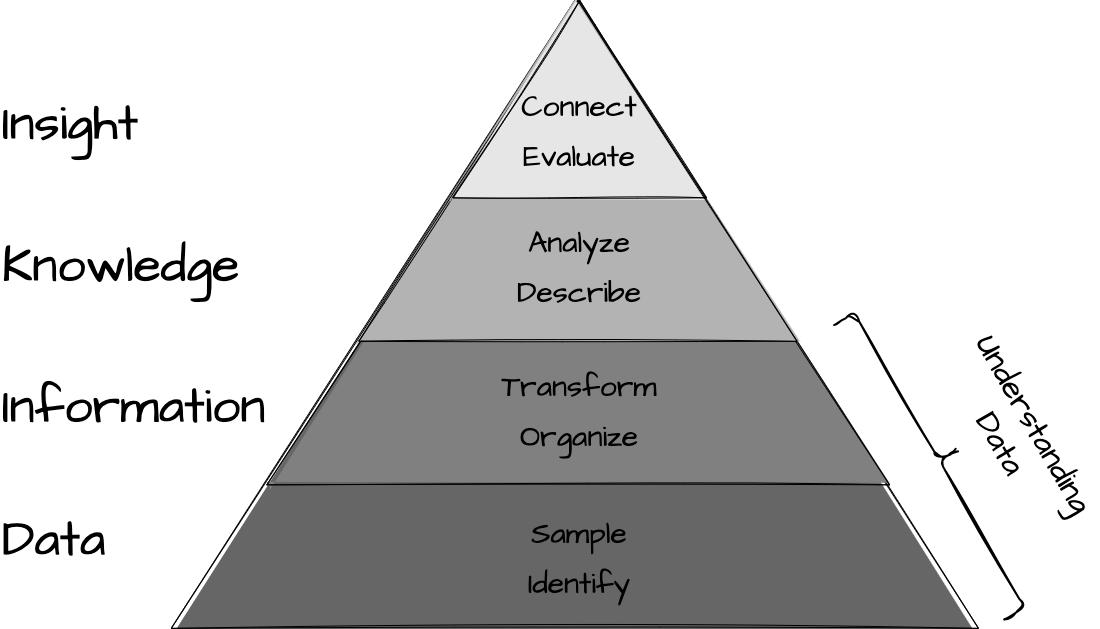
\includegraphics[width=0.75\textwidth,height=\textheight]{figures/understanding-data/ud-diki.drawio.png}

}

\caption{\label{fig-understanding-data-vis-sum}Understanding data:
visual summary}

\end{figure}

First a distinction is made between populations and samples, the latter
being a intentional and subjective selection of observations from the
world which attempt to represent the population of interest. The result
of this process is known as a corpus. Whether developing a corpus or
selecting an existing a corpus it is important to vet the sampling frame
for its applicability and viability as a resource for a given research
project.

Once a viable corpus is identified, then that corpus is converted into a
curated dataset which adopts the tidy dataset format where each column
is a variable, each row is an observation, and the intersection of
columns and rows contain values. This curated dataset serves to
establish the base informational relationships from which your research
will stem.

The curated dataset will most likely require transformations which may
include normalization, tokenization, recoding, generation, and/ or
merging to enhance the usefulness of the information to analysis. A
derived dataset or set of datasets will the result from this process.

Finally, documentation should be implemented at the acquisition,
curation, and transformation stages of the analysis project process. The
combination of data origin, data dictionary, and literate programming
files establishes documentation of the data and implementation steps to
ensure transparent and reproducible research.

\hypertarget{activities}{%
\section*{Activities}\label{activities}}
\addcontentsline{toc}{section}{Activities}

\markright{Activities}

In the following activities you will learn how to read, inspect, and
write data and datasets in R using reproducible strategies.

\begin{tcolorbox}[enhanced jigsaw, rightrule=.15mm, leftrule=.75mm, opacityback=0, arc=.35mm, colback=white, breakable, toprule=.15mm, bottomrule=.15mm, left=2mm]

\textbf{\faIcon{file-code} Recipe}

\textbf{What}:
\href{https://qtalr.github.io/qtalrkit/articles/recipe-2.html}{Reading,
inspecting, and writing data}\\
\textbf{How}: Read Recipe 2 and participate in the Hypothes.is online
social annotation.\\
\textbf{Why}: To use literate programming in Quarto to work with R
coding strategies for reading, inspecting, and writing datasets.

\end{tcolorbox}

\begin{tcolorbox}[enhanced jigsaw, rightrule=.15mm, leftrule=.75mm, opacityback=0, arc=.35mm, colback=white, breakable, toprule=.15mm, bottomrule=.15mm, left=2mm]

\textbf{\faIcon{flask} Lab}

\textbf{What}: \href{https://github.com/qtalr/lab-2}{Reading,
inspecting, and writing data}\\
\textbf{How}: Clone, fork, and complete the steps in Lab 2.\\
\textbf{Why}: To read datasets from packages and from plain-text files,
inspect and report characteristics of datasets, and write datasets to
plain-text files.

\end{tcolorbox}

\hypertarget{questions-1}{%
\section*{Questions}\label{questions-1}}
\addcontentsline{toc}{section}{Questions}

\markright{Questions}

\begin{tcolorbox}[enhanced jigsaw, rightrule=.15mm, leftrule=.75mm, opacityback=0, arc=.35mm, colback=white, breakable, toprule=.15mm, bottomrule=.15mm, left=2mm]

\textbf{Conceptual questions}

\begin{itemize}
\tightlist
\item
  What is the difference between a population and a sample?
\item
  Why is it important to vet a corpus before using it in a research
  project?
\item
  What is a curated dataset in the context of linguistic research?
\item
  What is the difference between a variable, an observation, and a
  value?
\item
  Why is it important to identify the informationasl types of variables
  in a dataset?
\item
  What kinds of transformations may be performed on a curated dataset to
  enhance its usefulness for analysis?
\item
  What is an transformed dataset and why is it important in linguistic
  research?
\item
  Why is documentation important in the process of conducting linguistic
  analysis?
\item
  How does a programmatic approach enhance documentation in linguistic
  research?
\item
  How does documenting the corpus data and the curated and derived
  datasets contribute to transparent and reproducible research in
  linguistics?
\end{itemize}

\end{tcolorbox}

\begin{tcolorbox}[enhanced jigsaw, rightrule=.15mm, leftrule=.75mm, opacityback=0, arc=.35mm, colback=white, breakable, toprule=.15mm, bottomrule=.15mm, left=2mm]

\faIcon{wrench} \textbf{Technical questions}

\begin{itemize}
\tightlist
\item
  Creating a sample corpus.
\item
  Writing a corpus documentation.
\item
  Converting a corpus to a derived dataset.
\item
  Writing a data dictionary.
\item
  Transforming a derived dataset.
\item
  Merging datasets.
\item
  Writing a dataset to disk.
\item
  Consider (an example dataset) and its data dictionary, write a script
  to read the dataset, inspect it, and write it to disk.
\item
  Consider a dataset and its data dictionary what appears to be the unit
  of analysis and the unit of observation?
\end{itemize}

\end{tcolorbox}

\hypertarget{sec-approaching-analysis}{%
\chapter{Approaching analysis}\label{sec-approaching-analysis}}

\begin{tcolorbox}[enhanced jigsaw, leftrule=.75mm, title=\textcolor{quarto-callout-tip-color}{\faLightbulb}\hspace{0.5em}{Draft}, coltitle=black, opacityback=0, titlerule=0mm, arc=.35mm, bottomtitle=1mm, opacitybacktitle=0.6, colframe=quarto-callout-tip-color-frame, rightrule=.15mm, toptitle=1mm, left=2mm, colback=white, breakable, toprule=.15mm, bottomrule=.15mm, colbacktitle=quarto-callout-tip-color!10!white]

Ready for review.

\end{tcolorbox}

\begin{quote}
Statistical thinking will one day be as necessary for efficient
citizenship as the ability to read and write.

--- H.G. Wells
\end{quote}

\begin{tcolorbox}[enhanced jigsaw, rightrule=.15mm, leftrule=.75mm, opacityback=0, arc=.35mm, colback=white, breakable, toprule=.15mm, bottomrule=.15mm, left=2mm]

\textbf{\faIcon{list-alt} Outcomes}

\begin{itemize}
\tightlist
\item
  Recall the fundamental concepts and principles of statistics in data
  analysis.
\item
  Articulate the roles of diagnostic, analytic, and interpretive
  statistics in quantitative analysis.
\item
  Compare the similarities and differences between analytic approaches
  to data analysis.
\end{itemize}

\end{tcolorbox}

In this chapter I will build on the notions of data and information from
the previous chapter. The aim of analysis is to derive knowledge from
information, the next step in the DIKI Hierarchy. Where the creation of
information from data involves human intervention and conscious
decisions, as we have seen, deriving knowledge from information involves
another level of intervention. The goal is to break down complex
information into simpler components which are more readily
interpretable. In what follows, we will cover the main steps in the
process of analysis. The first is to inspect the data to ensure its
quality and understand its characteristics. The second is to interrogate
the data to uncover patterns and relationships and interpret the
findings. To conclude this chapter I will outline methods to and the
importance of communicating the analysis results and procedure in a
transparent and reproducible manner.

\begin{tcolorbox}[enhanced jigsaw, rightrule=.15mm, leftrule=.75mm, opacityback=0, arc=.35mm, colback=white, breakable, toprule=.15mm, bottomrule=.15mm, left=2mm]

\textbf{\faIcon{terminal} Swirl lesson}

\textbf{What}: \href{https://github.com/qtalr/swirl}{Data
visualization}\\
\textbf{How}: In the R Console pane load \texttt{swirl}, run
\texttt{swirl()}, and follow prompts to select the lesson.\\
\textbf{Why}: To explore data visually in text and in graphics.

\end{tcolorbox}

\hypertarget{sec-aa-diagnose}{%
\section{Diagnose}\label{sec-aa-diagnose}}

The purpose of diagnostic measures is to inspect your data to ensure its
quality and understand its characteristics. There are two primary types
of diagnostic measures: verfication and description. Verification
methods are applied to catch missing or erroneous data while descriptive
methods are used to gain a better understanding of the data. Although
treated in two separate sections, in practice these methods are
complementary and are often addressed in tandem.

To ground this discussion I will introduce a new dataset. This dataset
is drawn from the Barcelona English Language Corpus (BELC)
(\protect\hyperlink{ref-Munoz2006}{Muñoz 2006}), which is found in the
TalkBank repository. I've selected the ``Written composition'' task from
this corpus which contains 80 writing samples from 36 second language
learners of English at different ages. Participants were given the task
of writing for 15 minutes on the topic of ``Me: my past, present and
future''. Data was collected for participants from one to three times
over the course of seven years (at 10, 12, 16, and 17 years of age).

In Table~\ref{tbl-aa-belc-dd} we see the data dictionary for the BELC
dataset which reflects structural and transformational steps I've done
so we start with a tidy dataset with \texttt{word} as the unit of
observation.

\hypertarget{tbl-aa-belc-dd}{}
\begin{longtable}[]{@{}
  >{\raggedright\arraybackslash}p{(\columnwidth - 6\tabcolsep) * \real{0.0962}}
  >{\raggedright\arraybackslash}p{(\columnwidth - 6\tabcolsep) * \real{0.2692}}
  >{\raggedright\arraybackslash}p{(\columnwidth - 6\tabcolsep) * \real{0.5000}}
  >{\raggedright\arraybackslash}p{(\columnwidth - 6\tabcolsep) * \real{0.1346}}@{}}
\caption{\label{tbl-aa-belc-dd}Data dictionary for the BELC
dataset.}\tabularnewline
\toprule\noalign{}
\begin{minipage}[b]{\linewidth}\raggedright
variable
\end{minipage} & \begin{minipage}[b]{\linewidth}\raggedright
name
\end{minipage} & \begin{minipage}[b]{\linewidth}\raggedright
description
\end{minipage} & \begin{minipage}[b]{\linewidth}\raggedright
variable\_type
\end{minipage} \\
\midrule\noalign{}
\endfirsthead
\toprule\noalign{}
\begin{minipage}[b]{\linewidth}\raggedright
variable
\end{minipage} & \begin{minipage}[b]{\linewidth}\raggedright
name
\end{minipage} & \begin{minipage}[b]{\linewidth}\raggedright
description
\end{minipage} & \begin{minipage}[b]{\linewidth}\raggedright
variable\_type
\end{minipage} \\
\midrule\noalign{}
\endhead
\bottomrule\noalign{}
\endlastfoot
part\_id & Participant ID & Unique identifier for each participant &
categorical \\
sex & Participant's sex & Sex of the participant & categorical \\
group & Time group & Longitudinal group to which the participant belongs
& ordinal \\
month\_age & Participant's age in months & Age of the participant in
months & numeric \\
utt\_id & Utterance ID & Unique identifier for each utterance &
numeric \\
word\_id & Word ID & Unique identifier for each word within an utterance
& numeric \\
word & Word & The word spoken by the participant & categorical \\
lemma & Word lemma & Base form of the word & categorical \\
pos & Part of speech & Grammatical category of the word & categorical \\
\end{longtable}

The data dictionary provides a easily accessible overview of the
dataset. This includes a human-readable mapping from variable names to
variable descriptions. Further, it provides information about the type
of variable (e.g., categorical, ordinal, numeric). As we will see the
informational type of variables is key to diagnostic measures, as well
as all other components of analysis.

\hypertarget{sec-aa-verfiy}{%
\subsection{Verify}\label{sec-aa-verfiy}}

Although a dataset has undergone curation and transformation, it is
still important to verify the data. This is a process of checking the
data to ensure that it is accurate and complete. In the case that it is
not, consideration should be given to how to address the issues.

The most basic and usually the first step is to check for
\textbf{missing data} to ensure that all necessary data points are
present. In Table~\ref{tbl-aa-belc-skim-missing}, there are missing
values for the \texttt{lemma} and \texttt{pos} variables in the BELC
dataset.

\hypertarget{tbl-aa-belc-skim-missing}{}
\begin{longtable}[]{@{}llrr@{}}
\caption{\label{tbl-aa-belc-skim-missing}Summary output for missing
values in the BELC dataset.}\tabularnewline
\toprule\noalign{}
variable & type & n\_missing & complete\_rate \\
\midrule\noalign{}
\endfirsthead
\toprule\noalign{}
variable & type & n\_missing & complete\_rate \\
\midrule\noalign{}
\endhead
\bottomrule\noalign{}
\endlastfoot
part\_id & character & 0 & 1.000 \\
sex & character & 0 & 1.000 \\
group & character & 0 & 1.000 \\
word & character & 0 & 1.000 \\
lemma & character & 79 & 0.985 \\
pos & character & 23 & 0.996 \\
month\_age & numeric & 0 & 1.000 \\
utt\_id & numeric & 0 & 1.000 \\
word\_id & numeric & 0 & 1.000 \\
\end{longtable}

There are two primary approaches to dealing with missing data: deletion
and recoding. Since these missing values account for only 1.5\% and
0.4\% of the data respectively, we might be safe to remove these
observations. Another approach is to recode the missing values by either
applying a unique value for missing values (e.g., \texttt{NULL}) or by
imputing values. Imputing values is usually done by replacing missing
values with some middle-of-the-road value (e.g., mean, median, mode),
but other, more nuanced approaches are possible.

\begin{tcolorbox}[enhanced jigsaw, rightrule=.15mm, leftrule=.75mm, opacityback=0, arc=.35mm, colback=white, breakable, toprule=.15mm, bottomrule=.15mm, left=2mm]

\textbf{\faIcon{medal} Dive deeper}

For more information on missing data, see the \faIcon{wrench} in this
book.

\end{tcolorbox}

In either case, it is important to consider the implications of missing
data for the analysis. For example, if the missing data is not at random
or include a sizeable portion of the values of interest, then the
analysis may be biased.

Value coding schemes, annotation errors, or other issues may result in
\textbf{anomalies} in the data. These are values that are unusual,
unexpected, or inconsistent with the rest of the data or effect the
treatment of the data for the particular analysis to be performed.

For categorical variables, this may include values that are not expected
or are not in the set of values that are expected. A summary of the
values for a given variable can be used as a first step to identify
anomalies. In Table~\ref{tbl-aa-belc-skim-categorical}, we see the
minimum and maximum number of characters and the number of unique values
for each categorical variable in the BELC dataset.

\hypertarget{tbl-aa-belc-skim-categorical}{}
\begin{longtable}[]{@{}lrrr@{}}
\caption{\label{tbl-aa-belc-skim-categorical}Summary output for
categorical variables in the BELC dataset.}\tabularnewline
\toprule\noalign{}
variable & min\_chars & max\_chars & num\_unique \\
\midrule\noalign{}
\endfirsthead
\toprule\noalign{}
variable & min\_chars & max\_chars & num\_unique \\
\midrule\noalign{}
\endhead
\bottomrule\noalign{}
\endlastfoot
part\_id & 3 & 3 & 36 \\
sex & 4 & 6 & 2 \\
group & 2 & 2 & 4 \\
word & 1 & 20 & 913 \\
lemma & 1 & 20 & 774 \\
pos & 1 & 9 & 38 \\
\end{longtable}

From our knowledge of the data, we can gauge whether these values are
expected. For example, \texttt{sex} has two values; likely corresponding
to some coding of `male' and `female'. The variable \texttt{part\_id}
has 36 distinct values, which is expected since there are 36
participants and \texttt{group} has four, corresponding to the
longitudinal time groups. It is also possible to gauge the expected
values for \texttt{lemma} as we know that these are the base words and
should be less than the number of words in the dataset.

Further verfication of the categorical variables is need, of course.
This may include aggregating the data to see the distribution of values
and/ or checking the values against the documentation.

Let's now consider numeric variables. Numeric variables, by their very
nature, do not lend themselves to the same type of summary used for
categorical variables (\emph{i.e.} character lengths, number of unique
values, or aggregation) to detect anomalies. For numeric variables there
are two types of anomalies that we will consider: outliers and errors in
coding. \textbf{Outliers} are anomalies that are extreme values that are
not representative of the great majority of the data points. To
determine what is extreme, we need to consider the distribution of the
data, that is, the range of values and the frequency of values. It is
rarely the case that we can eyeball the distribution of the data based
on raw values. Instead, a combination of summary statistics and
visualizations are used to determine the distribution of the data. For
this reason, the detection of outliers is often carried out as part of
the descriptive assessment of the data, as we will see in
Section~\ref{sec-aa-describe}.

On the other hand, coding anomalies are values that are not expected or
are not in the set of values that are expected. These can sometimes be
detected by visual inspection of the data. For example, in
Table~\ref{tbl-aa-belc-numeric}, we see the first 10 observations for
each variable in the BELC dataset.

\hypertarget{tbl-aa-belc-numeric}{}
\begin{longtable}[]{@{}
  >{\raggedright\arraybackslash}p{(\columnwidth - 16\tabcolsep) * \real{0.1081}}
  >{\raggedright\arraybackslash}p{(\columnwidth - 16\tabcolsep) * \real{0.0946}}
  >{\raggedright\arraybackslash}p{(\columnwidth - 16\tabcolsep) * \real{0.0811}}
  >{\raggedleft\arraybackslash}p{(\columnwidth - 16\tabcolsep) * \real{0.1351}}
  >{\raggedleft\arraybackslash}p{(\columnwidth - 16\tabcolsep) * \real{0.0946}}
  >{\raggedleft\arraybackslash}p{(\columnwidth - 16\tabcolsep) * \real{0.1081}}
  >{\raggedright\arraybackslash}p{(\columnwidth - 16\tabcolsep) * \real{0.1351}}
  >{\raggedright\arraybackslash}p{(\columnwidth - 16\tabcolsep) * \real{0.1351}}
  >{\raggedright\arraybackslash}p{(\columnwidth - 16\tabcolsep) * \real{0.1081}}@{}}
\caption{\label{tbl-aa-belc-numeric}First 10 observations for variables
in the BELC dataset.}\tabularnewline
\toprule\noalign{}
\begin{minipage}[b]{\linewidth}\raggedright
part\_id
\end{minipage} & \begin{minipage}[b]{\linewidth}\raggedright
sex
\end{minipage} & \begin{minipage}[b]{\linewidth}\raggedright
group
\end{minipage} & \begin{minipage}[b]{\linewidth}\raggedleft
month\_age
\end{minipage} & \begin{minipage}[b]{\linewidth}\raggedleft
utt\_id
\end{minipage} & \begin{minipage}[b]{\linewidth}\raggedleft
word\_id
\end{minipage} & \begin{minipage}[b]{\linewidth}\raggedright
word
\end{minipage} & \begin{minipage}[b]{\linewidth}\raggedright
lemma
\end{minipage} & \begin{minipage}[b]{\linewidth}\raggedright
pos
\end{minipage} \\
\midrule\noalign{}
\endfirsthead
\toprule\noalign{}
\begin{minipage}[b]{\linewidth}\raggedright
part\_id
\end{minipage} & \begin{minipage}[b]{\linewidth}\raggedright
sex
\end{minipage} & \begin{minipage}[b]{\linewidth}\raggedright
group
\end{minipage} & \begin{minipage}[b]{\linewidth}\raggedleft
month\_age
\end{minipage} & \begin{minipage}[b]{\linewidth}\raggedleft
utt\_id
\end{minipage} & \begin{minipage}[b]{\linewidth}\raggedleft
word\_id
\end{minipage} & \begin{minipage}[b]{\linewidth}\raggedright
word
\end{minipage} & \begin{minipage}[b]{\linewidth}\raggedright
lemma
\end{minipage} & \begin{minipage}[b]{\linewidth}\raggedright
pos
\end{minipage} \\
\midrule\noalign{}
\endhead
\bottomrule\noalign{}
\endlastfoot
L01 & female & T2 & 153 & 0 & 0 & I & I & pro:sub \\
L01 & female & T2 & 153 & 0 & 1 & was & be & cop \\
L01 & female & T2 & 153 & 0 & 2 & born & born & adj \\
L01 & female & T2 & 153 & 0 & 3 & in & in & prep \\
L01 & female & T2 & 153 & 0 & 4 & Barcelona & Barcelona & n:prop \\
L01 & female & T2 & 153 & 0 & 5 & and & and & coord \\
L01 & female & T2 & 153 & 0 & 6 & I & I & pro:sub \\
L01 & female & T2 & 153 & 0 & 7 & live & live & v \\
L01 & female & T2 & 153 & 0 & 8 & in & in & prep \\
L01 & female & T2 & 153 & 0 & 9 & Barcelona & Barcelona & n:prop \\
\end{longtable}

Leaving \texttt{month\_age} aside, we see that the other two numeric
variables \texttt{utt\_id} and \texttt{word\_id} index utterances and
words respectively. However, in contrast to \texttt{part\_id} which is a
categorical variable as it serves as a unique identifier for each
participant, these variables are numeric as they serve to not only index
utterances and words but also to provide a measure of how many
utterances or words have been produced. Seen in this light, \texttt{0}
for the first value of \texttt{utt\_id} and \texttt{word\_id} is
unexpected. To adjust for this, we can add \texttt{1} to each value of
these variables.

\hypertarget{sec-aa-describe}{%
\subsection{Describe}\label{sec-aa-describe}}

The goal of descriptive statistics is to summarize the data in order to
understand and prepare the data for the analysis approach to be
performed. This is accomplished through a combination of statistic
measures and/ or tabular or graphic summaries. The choice of descriptive
statistics is guided by the type of data, as well as the question(s)
being asked of the data.

To that end, let's consider a reconfiguration of the BELC dataset, in
Table~\ref{tbl-aa-belc-reconfig}, which will provide a more illustrative
dataset.

\hypertarget{tbl-aa-belc-reconfig}{}
\begin{longtable}[]{@{}llllrrrr@{}}
\caption{\label{tbl-aa-belc-reconfig}First 10 observations of the
reconfigured BELC dataset.}\tabularnewline
\toprule\noalign{}
essay\_id & part\_id & sex & group & tokens & types & ttr & prop\_l2 \\
\midrule\noalign{}
\endfirsthead
\toprule\noalign{}
essay\_id & part\_id & sex & group & tokens & types & ttr & prop\_l2 \\
\midrule\noalign{}
\endhead
\bottomrule\noalign{}
\endlastfoot
E1 & L01 & female & T2 & 79 & 46 & 0.582 & 0.987 \\
E2 & L02 & female & T1 & 18 & 18 & 1.000 & 0.667 \\
E3 & L02 & female & T3 & 101 & 53 & 0.525 & 1.000 \\
E4 & L05 & female & T1 & 20 & 17 & 0.850 & 0.900 \\
E5 & L05 & female & T3 & 158 & 80 & 0.506 & 0.987 \\
E6 & L05 & female & T4 & 184 & 94 & 0.511 & 0.995 \\
E7 & L07 & male & T3 & 98 & 60 & 0.612 & 1.000 \\
E8 & L07 & male & T4 & 134 & 84 & 0.627 & 0.978 \\
E9 & L10 & female & T1 & 38 & 28 & 0.737 & 0.974 \\
E10 & L10 & female & T3 & 118 & 74 & 0.627 & 1.000 \\
\end{longtable}

In this new configuration, the unit of observation is now
\texttt{essay\_id}. Each of the following variable are attributes or
measures of this variable. The new variables in this dataset are
aggregates of the previous BELC dataset: \texttt{tokens} is the number
of total words, \texttt{types} is the number of unique words,
\texttt{ttr} is the ratio of unique words to total words. This is known
as the Type-Token Ratio and it is a standard metric for measuring
lexical diversity. Finally, the proportion of L2 words (English) to the
total words (tokens) is provided in \texttt{prop\_l2}.

In descriptive statistics, there are four basic questions that are asked
of each of the variables in the dataset. Each correspond to a different
type of descriptive measure.

\begin{enumerate}
\def\labelenumi{\arabic{enumi}.}
\tightlist
\item
  Central Tendency: Where do the data points tend to be located?
\item
  Dispersion: How spread out are the data points?
\item
  Distribution: What is the overall shape of of the data points?
\item
  Interdependence: How are these data points related to other data?
\end{enumerate}

\hypertarget{sec-aa-central-tendency}{%
\subsubsection{Central tendency}\label{sec-aa-central-tendency}}

The central tendency is measure which aims to summarize the data points
in a variable as the most representative, middle or most typical value.
There are three common measures of central tendency: the mode, mean and
median. Each differ in how they summarize the data points.

The \textbf{mode} is the value, or values, that appears most frequently
in a set of values. If there are multiple values with the highest
frequency, then the variable is said to be multimodal. The most
versatile of the central tendency measures as it can be applied to all
levels of measurement, although the mode is not often used for numeric
variables as it is not as informative as other measures.

The more common measures for numeric variables are the mean and the
median. The \textbf{mean} is a summary statistic calculated by summing
all the values and dividing by the number of values. The \textbf{median}
is calculated by sorting all the values in the variable and then
selecting the middle value. Given that the mean and median are
calculated differently, they will not always yield the same result.
Differences that appear between the mean and median will be of interest
to us later in this chapter.

\hypertarget{dispersion}{%
\subsubsection{Dispersion}\label{dispersion}}

The mean, median, and mode provide summary information where data points
tend to be located. However, they do not provide us with any
understanding as to how representative this value is. To provide this
context, the spread of the values around the central tendency, or
\textbf{dispersion}, is calculated.

For categorical variables, the spread is framed in terms of how balanced
the values are across the levels. One way to do this is to calculate the
(normalized) entropy. \textbf{Entropy} is a measure of uncertainty. The
more balanced the values are across the levels, the higher the entropy.
The less balanced the values are across the levels, the lower the
entropy. Normalized entropy scores range from 0 to 1, with 0 indicating
that all the values are the same and 1 indicating that all the values
are different.

The most common measure of dispersion for numeric variables is the
\textbf{standard deviation}. The standard deviation is calculated by
taking the square root of the variance. The \textbf{variance} is the
average of the squared differences from the mean. So, more succinctly,
the standard deviation is a measure of the spread of the values around
the mean. Where the standard deviation is anchored to the mean, the
\textbf{interquartile range} (IQR) is tied to the median. The median
represents the sorted middle of the values, in other words the 50th
percentile. The IQR is the difference between the 75th percentile and
the 25th percentile. Again, just as the mean and the median, the
standard deviation and the IQR are calculated in different ways, they
are not always the same.

Let's now consider the relevant central tendency and dispersion of the
variables in the BELC dataset in
Table~\ref{tbl-aa-belc-descriptive-stats}.

\begin{table}

\caption{\label{tbl-aa-belc-descriptive-stats}Central tendency and
dispersion of the variables in the BELC
dataset}\begin{minipage}[t]{0.50\linewidth}
\subcaption{\label{tbl-aa-belc-descriptive-stats-1}Categorical
variables}

{\centering 

\begin{tabular}[t]{llr}
\toprule
variable & top\_counts & norm\_entropy\\
\midrule
essay\_id & E1: 1, E10: 1, E11: 1, E12: 1 & 1.000\\
part\_id & L05: 3, L10: 3, L11: 3, L12: 3 & 0.983\\
sex & fem: 48, mal: 32 & 0.971\\
group & T1: 25, T3: 24, T2: 16, T4: 15 & 0.981\\
\bottomrule
\end{tabular}

}

\end{minipage}%
%
\begin{minipage}[t]{0.50\linewidth}
\subcaption{\label{tbl-aa-belc-descriptive-stats-2}Numeric variables}

{\centering 

\begin{tabular}[t]{lrrrr}
\toprule
variable & mean & median & sd & iqr\\
\midrule
tokens & 67.62 & 56.50 & 44.20 & 61.25\\
types & 41.85 & 38.50 & 23.03 & 31.50\\
ttr & 0.68 & 0.66 & 0.13 & 0.15\\
prop\_l2 & 0.96 & 0.99 & 0.10 & 0.03\\
\bottomrule
\end{tabular}

}

\end{minipage}%

\end{table}

In Table~\ref{tbl-aa-belc-descriptive-stats-1} we see the measures for
categorical variables. The \texttt{top\_counts} variable gives us a
short list of the most frequent levels of the variable. From
\texttt{top\_count} we can gather whether the variable has one mode or
is multimodel. Both \texttt{essay\_id} and \texttt{part\_id} have the
same most frequent value for the levels listed. On the other hand,
\texttt{sex} and \texttt{group} have a single mode. We can also
appreciate the dispersion of these variables based on the
\texttt{norm\_entropy} of each variable. \texttt{essay\_id} is
completely balanced across the levels, so it has a normalized entropy of
1. the other variables are not as balanced, but still quite balanced as
the normalized entropy is close to 1.

In Table~\ref{tbl-aa-belc-descriptive-stats-2} the numeric variables
have a column for the mean, median, standard deviation, and IQR for
each. The variable \texttt{tokens} has a larger difference between the
mean and median than the other variables and the standard deviation is
relatively large suggesting that the values are more spread out around
the mean. In the case of \texttt{ttr} the mean and median are quite
close and the standard deviation is relatively small suggesting that the
values are more tightly clustered around the mean.

When interpreting these summary values, it is important to only directly
compare column-wise. That is, focusing only on a single variable, not
across variables. Each variable, as is, is measured on a different scale
and only relative to itself can we make sense of the values.

However, we can transform the central tendency and dispersion scores for
numeric variables to make them more comparable by standardizing the
scale of the values. \textbf{Standardization} is a scale-based
transformation that changes the scale of the values to a common scale,
or \emph{z-scores}. It involves two separate transformations: centering
and scaling. \textbf{Centering} is a transformation that subtracts the
mean or median from each value. The result is a mean and median of zero.
\textbf{Scaling} is a transformation that divides each value by the
standard deviation or IQR.

In Table~\ref{tbl-aa-belc-descriptive-stats-standardized}, we see the
same summary statistics as in
Table~\ref{tbl-aa-belc-descriptive-stats-2}, but the values have been
standardized for the mean and standard deviation. The mean is now zero
and the standard deviation is one. This allows us to compare the median
and IQR of the variables more directly.

\hypertarget{tbl-aa-belc-descriptive-stats-standardized}{}
\begin{longtable}[]{@{}lrrrr@{}}
\caption{\label{tbl-aa-belc-descriptive-stats-standardized}Standardized
central tendency and dispersion of numeric variables}\tabularnewline
\toprule\noalign{}
variable & mean & median & sd & iqr \\
\midrule\noalign{}
\endfirsthead
\toprule\noalign{}
variable & mean & median & sd & iqr \\
\midrule\noalign{}
\endhead
\bottomrule\noalign{}
\endlastfoot
tokens & 0 & -0.25 & 1 & 1.39 \\
types & 0 & -0.15 & 1 & 1.37 \\
ttr & 0 & -0.19 & 1 & 1.14 \\
prop\_l2 & 0 & 0.25 & 1 & 0.27 \\
\end{longtable}

One more caveat to keep in mind is that we need to be mindful of the
nature of the data being standardized and what the standardized values
mean. For example, the variables \texttt{tokens} and \texttt{types} were
originally counts. But the standardized values are not interpretable as
counts, they are now on a different scale --specifically a z-score
scale. In the same way since the \texttt{ttr} and \texttt{prop\_l2}
variables were originally proportions, the standardized values are also
not interpretable as proportions. One additional twist, however, is that
the original scales for these pairs of variables were not the same:
\texttt{tokens} and \texttt{types} were counts, but \texttt{ttr} and
\texttt{prop\_l2} were proportions. So, even though the standardized
values are on the same scale, they are not directly comparable.

Beyond comparing central tendency and dispersion across variables,
standarization is useful for analytic statistics to mitigate the
influence of variables with large values. In some cases, the statistical
method will require standardization of variables before analysis.

\hypertarget{distributions}{%
\subsubsection{Distributions}\label{distributions}}

Summary statistics of the central tendency and dispersion of a variable
provide a sense of the most representative value and how spread out the
data is around this value. However, to gain a more comprehensive
understanding of the variable, it is key to consider the frequencies of
all the data points. The \textbf{distribution} of a variable is the
pattern or shape of the data that emerges when the frequencies of all
data points are considered. This can reveal patterns that might not be
immediately apparent from summary statistics alone. Understanding the
frequency and distribution of data points is vital as it informs
subsequent choices of statistical analysis and evaluative methods,
ensuring they are appropriate for the specific characteristics of the
data.

When assessing the distribution of categorical variables, we can use a
frequency table or bar plot. A \textbf{frequency table} is a useful
method to display the frequency and proportion of each level in a
categorical variable in a clear and concise manner. In
Table~\ref{tbl-aa-belc-frequency-table} we see the frequency table for
the variable \texttt{sex}.

\hypertarget{tbl-aa-belc-frequency-table}{}
\begin{longtable}[]{@{}lrr@{}}
\caption{\label{tbl-aa-belc-frequency-table}Frequency table for the
variable \texttt{sex}.}\tabularnewline
\toprule\noalign{}
sex & frequency & proportion \\
\midrule\noalign{}
\endfirsthead
\toprule\noalign{}
sex & frequency & proportion \\
\midrule\noalign{}
\endhead
\bottomrule\noalign{}
\endlastfoot
female & 48 & 0.6 \\
male & 32 & 0.4 \\
\end{longtable}

A \textbf{bar plot} is a type of plot where the x-axis is a categorical
variable and the y-axis is the frequency of the values. The frequency is
represented by the height of the bar. The variables can be ordered by
frequency, alphabetically, or some other order.
Figure~\ref{fig-aa-belc-barplots} is a bar chart for the variables
\texttt{sex}, \texttt{group}, and \texttt{part\_id}, ordered
alphabetically.

\begin{figure}

\begin{minipage}[t]{0.33\linewidth}

{\centering 

\raisebox{-\height}{

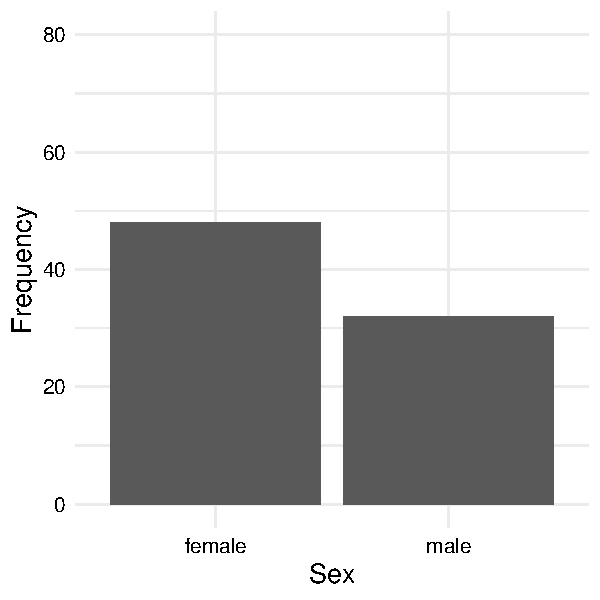
\includegraphics{approaching-analysis_files/figure-pdf/fig-aa-belc-barplots-1.pdf}

}

}

\subcaption{\label{fig-aa-belc-barplots-1}Sex}
\end{minipage}%
%
\begin{minipage}[t]{0.33\linewidth}

{\centering 

\raisebox{-\height}{

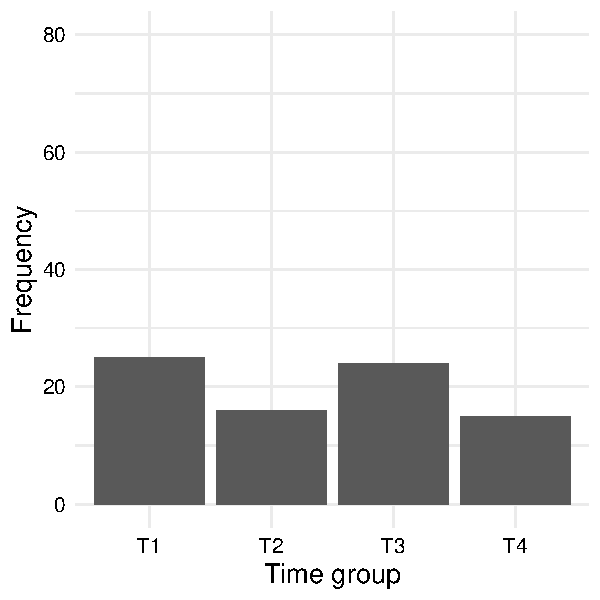
\includegraphics{approaching-analysis_files/figure-pdf/fig-aa-belc-barplots-2.pdf}

}

}

\subcaption{\label{fig-aa-belc-barplots-2}Time group}
\end{minipage}%
%
\begin{minipage}[t]{0.33\linewidth}

{\centering 

\raisebox{-\height}{

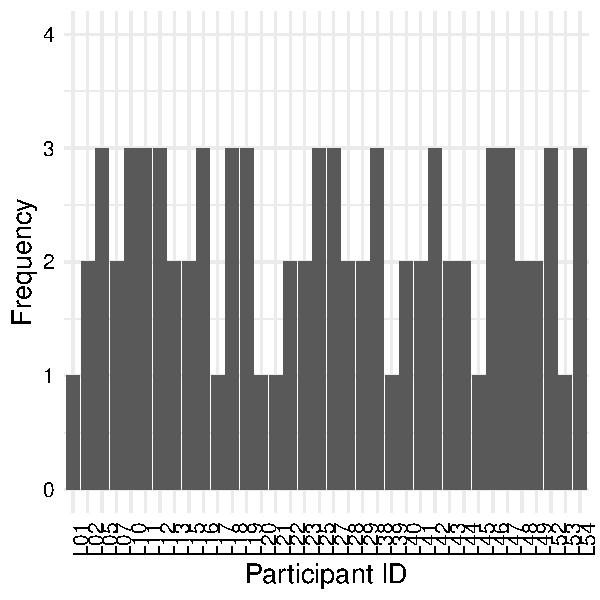
\includegraphics{approaching-analysis_files/figure-pdf/fig-aa-belc-barplots-3.pdf}

}

}

\subcaption{\label{fig-aa-belc-barplots-3}Participant ID}
\end{minipage}%

\caption{\label{fig-aa-belc-barplots}Bar plots for categorical variables
\texttt{sex}, \texttt{group}, \texttt{part\_id} in the BELC dataset.}

\end{figure}

So for a frequency table or barplot, we can see the frequency of each
level of a categorical variable. This gives us some knowledge about the
BELC dataset: there are more girls in the dataset, more essays appear in
first and third time groups, and the number of essays written by each
participant is scattered from one to three. If we were to see any
clearly loopsided categories, this would be a sign of imbalance in the
data and we would need to consider how this might impact our analysis.

\begin{tcolorbox}[enhanced jigsaw, rightrule=.15mm, leftrule=.75mm, opacityback=0, arc=.35mm, colback=white, breakable, toprule=.15mm, bottomrule=.15mm, left=2mm]

\textbf{\faIcon{lightbulb} Consider this}

The goal of descriptive statistics is to summarize the data in a way
that is meaningful and interpretable. With this in mind, compare the
frequency table in \ref{tbl-aa-belc-frequency-table} and bar plot in
\ref{fig-aa-belc-barplots-1}. Does one provide a more interpretable
summary of the data? Why or why not? Are there any other ways you might
communicate this distribution more effectively?

\end{tcolorbox}

For numeric variables, understanding the distribution is more complex,
and also more important. In essence, however, we are assessing two
things: the appearance of outliers in relation to and the overall shape
of the distribution.

Now, a frequency table, as in Table~\ref{tbl-aa-belc-frequency-table},
does not summarize the distribution of a numeric variable in a concise,
readily human-consumable format. Instead, the distribution of a numeric
variable is best understood visually.

The most common visualizations of the distribution of a numeric variable
are histograms and density plots. \textbf{Histograms} are a type of bar
plot where the x-axis is a numeric variable and the y-axis is the
frequency of the values falling within a determined range of values, or
bins. The frequency of values within each bin is represented by the
height of the bars. \textbf{Density plots} are a smoothed version of
histograms. The y-axis of a density plot is the probability of the
values. When frequent values appear closely together, the plot line is
higher. When the frequency of values is lower or more spread out, the
plot line is lower. An example of these plots is show in
Figure~\ref{fig-aa-belc-histogram-density-tokens} for the variable
\texttt{tokens}.

\begin{figure}

\begin{minipage}[t]{0.50\linewidth}

{\centering 

\raisebox{-\height}{

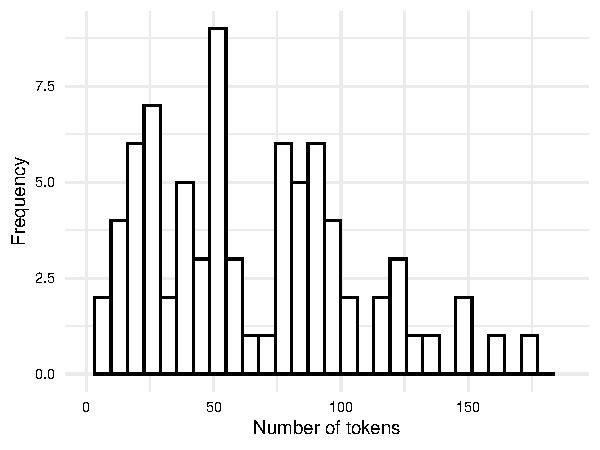
\includegraphics{approaching-analysis_files/figure-pdf/fig-aa-belc-histogram-density-tokens-1.pdf}

}

}

\subcaption{\label{fig-aa-belc-histogram-density-tokens-1}Histogram}
\end{minipage}%
%
\begin{minipage}[t]{0.50\linewidth}

{\centering 

\raisebox{-\height}{

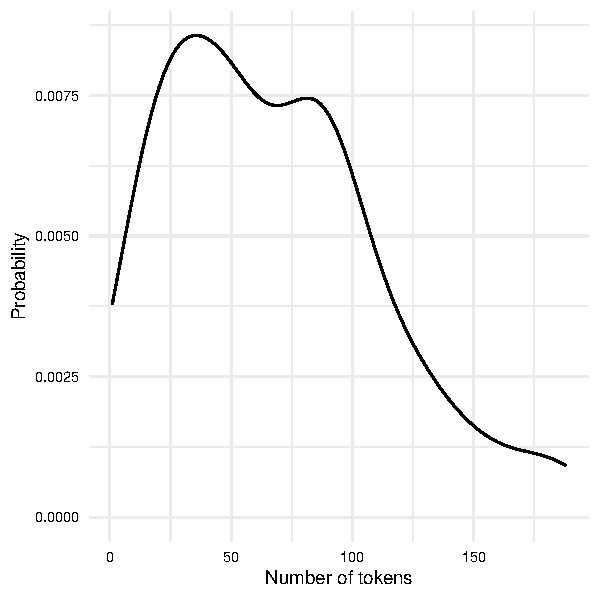
\includegraphics{approaching-analysis_files/figure-pdf/fig-aa-belc-histogram-density-tokens-2.pdf}

}

}

\subcaption{\label{fig-aa-belc-histogram-density-tokens-2}Density plot}
\end{minipage}%

\caption{\label{fig-aa-belc-histogram-density-tokens}Distribution plots
for the variable \texttt{tokens}.}

\end{figure}

Both the histogram in
Figure~\ref{fig-aa-belc-histogram-density-tokens-1} and the density plot
in Figure~\ref{fig-aa-belc-histogram-density-tokens-2} show the
distribution of the variable \texttt{tokens} in slightly different ways
which translate into trade-offs in terms of interpretability.

The histogram shows the frequency of the values in bins. The number of
bins and/ or binwidth can be changed for more or less granularity. A
rough grain histogram shows the general shape of the distribution, but
it is difficult to see the details of the distribution. A fine grain
histogram shows the details of the distribution, but it is difficult to
see the general shape of the distribution. The density plot shows the
general shape of the distribution, but it hides the details of the
distribution. Given this trade-off, it is often useful explore outliers
with histograms and the overall shape of the distribution with density
plots.

In Figure~\ref{fig-aa-belc-histograms} we see histograms for the
variables \texttt{tokens}, \texttt{types}, and \texttt{ttr}.

\begin{figure}

\begin{minipage}[t]{0.33\linewidth}

{\centering 

\raisebox{-\height}{

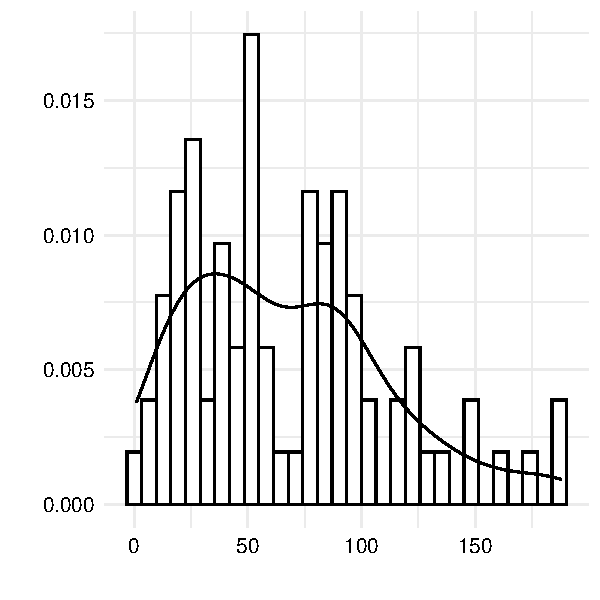
\includegraphics{approaching-analysis_files/figure-pdf/fig-aa-belc-histograms-1.pdf}

}

}

\subcaption{\label{fig-aa-belc-histograms-1}Number of tokens}
\end{minipage}%
%
\begin{minipage}[t]{0.33\linewidth}

{\centering 

\raisebox{-\height}{

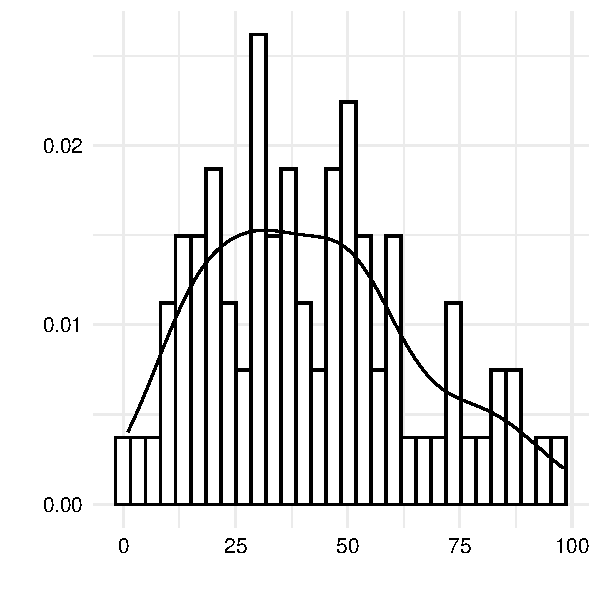
\includegraphics{approaching-analysis_files/figure-pdf/fig-aa-belc-histograms-2.pdf}

}

}

\subcaption{\label{fig-aa-belc-histograms-2}Number of types}
\end{minipage}%
%
\begin{minipage}[t]{0.33\linewidth}

{\centering 

\raisebox{-\height}{

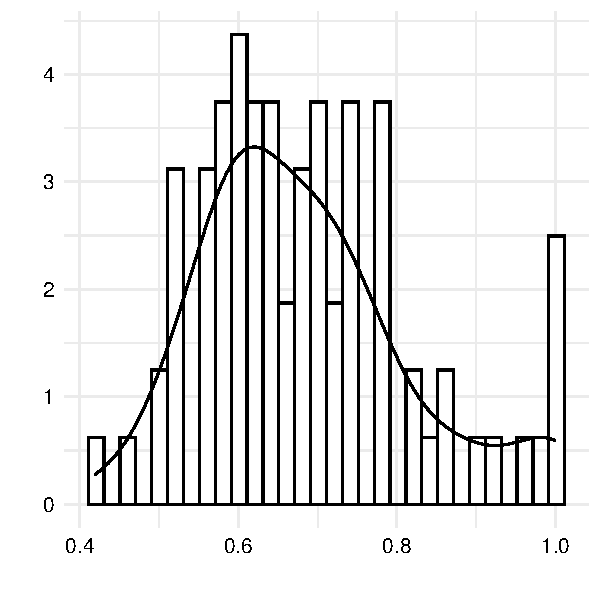
\includegraphics{approaching-analysis_files/figure-pdf/fig-aa-belc-histograms-3.pdf}

}

}

\subcaption{\label{fig-aa-belc-histograms-3}Type-token ratio score}
\end{minipage}%

\caption{\label{fig-aa-belc-histograms}Histograms for numeric variables
\texttt{tokens}, \texttt{types}, and \texttt{ttr}.}

\end{figure}

Focusing on the details captured in the histogram we are better able to
detect potential outliers. Outliers can reflect valid values that are
simply extreme or they can reflect something erroneous in the data. To
distinguish between these two possibilities, it is important to know the
context of the data. Take, for example,
Figure~\ref{fig-aa-belc-histograms-3}. We see that there is a bin near
the value 1.0. Given that the type-token ratio is a ratio of the number
of types to the number of tokens, it is unlikely that the type-token
ratio would be exactly 1.0 as this would mean that every word in an
essay is unique. Another, less dramatic, example is the bin to the far
right of Figure~\ref{fig-aa-belc-histograms-1}. In this case, the bin
represents the number of tokens in an essay. An uptick in the number of
essays with a large number of tokens is not surprising and would not
typically be considered an outlier. On the other hand, consider the bin
near the value 0 in the same plot. It is unlikely that a true essay
would have 0, or near 0, words and therefore a closer look at the data
is warranted.

It is important to recognize that outliers contribute undue influence to
overall measures of central tendency and dispersion. To appreciate this,
let's consider another helpful visualization called a \textbf{boxplot}.
A boxplot is a visual representation which aims to represent the central
tendency, dispersion, and distribution of a numeric variable in one
plot.

\begin{figure}[H]

{\centering 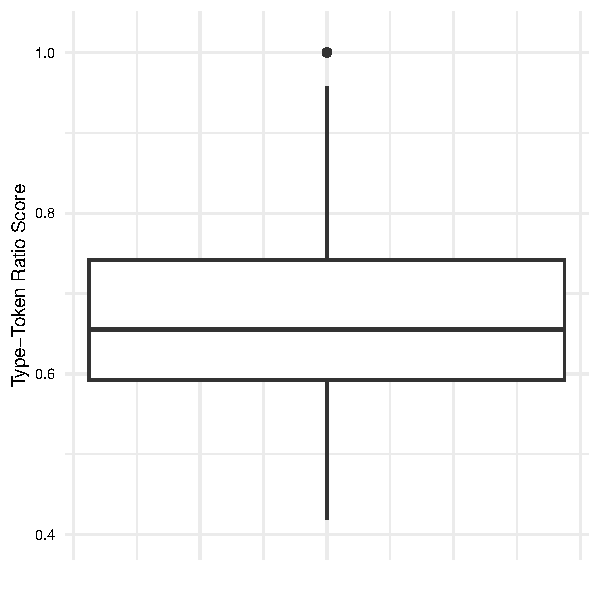
\includegraphics{approaching-analysis_files/figure-pdf/fig-aa-belc-boxplot-1.pdf}

}

\caption{\label{fig-aa-belc-boxplot}Boxplot for the variable
\texttt{ttr}.}

\end{figure}

In Figure~\ref{fig-aa-belc-boxplot} we see a boxplot for \texttt{ttr}
variable. The box in the middle of the plot represents the interquartile
range (IQR) which is the range of values between the first quartile and
the third quartile. The solid line in the middle of the box represents
the median. The lines extending from the box are called `whiskers' and
provide the range of values which are within 1.5 times the IQR. Values
outside of this range are plotted as individual points.

Now let's consider boxplots from another angle. In
Figure~\ref{fig-aa-belc-histogram-boxplot-comparison-2} I've plotted the
boxplot horizontally, right below the histogram in
Figure~\ref{fig-aa-belc-histogram-boxplot-comparison-1}. In this view,
we can see that a boxplot is a simplifed histogram augmented with
central tendency and dispersion statistics. While histograms focus on
the frequency distribution of data points, boxplots focus on the data's
quartiles and potential outliers.

\begin{figure}

\begin{minipage}[t]{\linewidth}

{\centering 

\raisebox{-\height}{

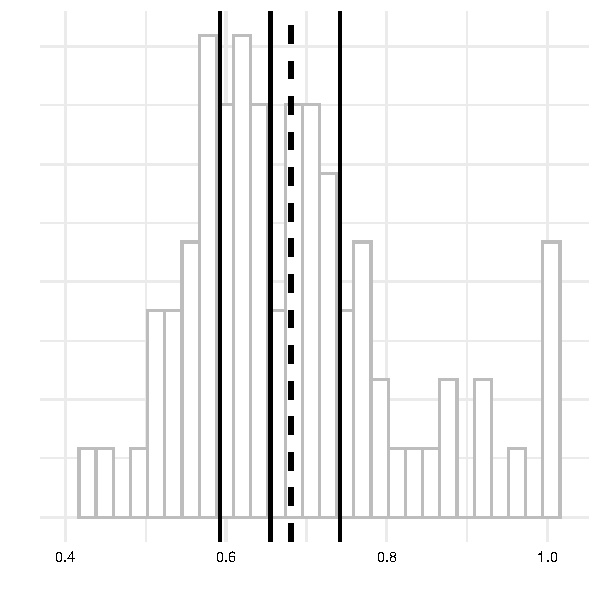
\includegraphics{approaching-analysis_files/figure-pdf/fig-aa-belc-histogram-boxplot-comparison-1.pdf}

}

}

\subcaption{\label{fig-aa-belc-histogram-boxplot-comparison-1}Histogram}
\end{minipage}%
\newline
\begin{minipage}[t]{\linewidth}

{\centering 

\raisebox{-\height}{

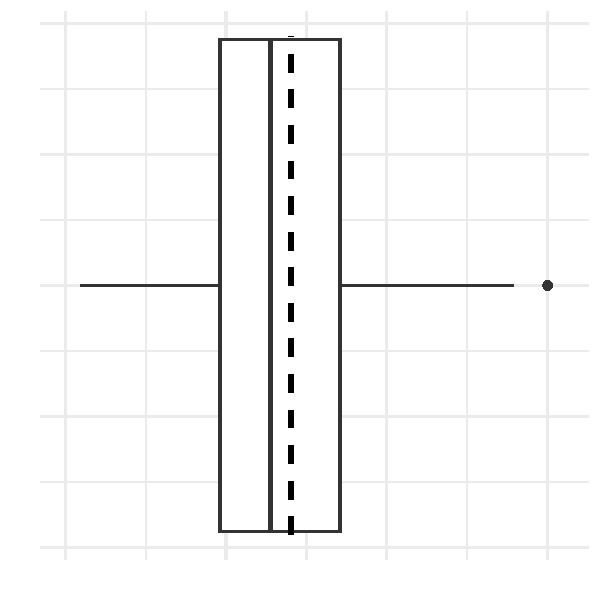
\includegraphics{approaching-analysis_files/figure-pdf/fig-aa-belc-histogram-boxplot-comparison-2.pdf}

}

}

\subcaption{\label{fig-aa-belc-histogram-boxplot-comparison-2}Boxplot
(horizontal)}
\end{minipage}%

\caption{\label{fig-aa-belc-histogram-boxplot-comparison}Histogram and
boxplot for the variable \texttt{ttr}.}

\end{figure}

I've added a dashed line in
Figure~\ref{fig-aa-belc-histogram-boxplot-comparison-1} and
Figure~\ref{fig-aa-belc-histogram-boxplot-comparison-2} to signal the
mean in this set of plots, but it is not typically included. I include
the dashed line to make a point: the mean is more sensitive to outliers
than the median. As I pointed out in
Section~\ref{sec-aa-central-tendency}, the mean is the sum of all values
divided by the number of values. If there are extreme values, the mean
will be pulled in the direction of the extreme values. The median,
however, is the middle value and a few extreme values have less effect.
So, when central tendency is reported, if there is a sizeable difference
between the mean and the median, measures of dispersion will be larger
and the direction of the difference can be used to infer the presence of
outliers.

Returning to outliers, it is important to address them to safeguard the
accuracy of the analysis. There are two main ways to address outliers:
1) transform the data and 2) eliminate observations with outliers
(\textbf{trimming}). Trimming is more extreme as it removes data but can
be the best approach for true outliers. Transforming the data is an
approach to mitigating the influence of extreme but valid values.
\textbf{Transformation} involves applying a mathematical function to the
data which changes the scale and/ or shape of the distribution, but does
not remove data nor does it change the relative order of the values.

In Figure~\ref{fig-aa-belc-histogram-density-trimmed}, we see two
boxplots. Figure~\ref{fig-aa-belc-boxplot-trimmed-1} is the original
\texttt{ttr} data and Figure~\ref{fig-aa-belc-boxplot-trimmed-2}
reflects the data trimmed to remove outliers. In this case, we have
removed essays with a type-token ratio of 1.

\begin{figure}

\begin{minipage}[t]{0.50\linewidth}

{\centering 

\raisebox{-\height}{

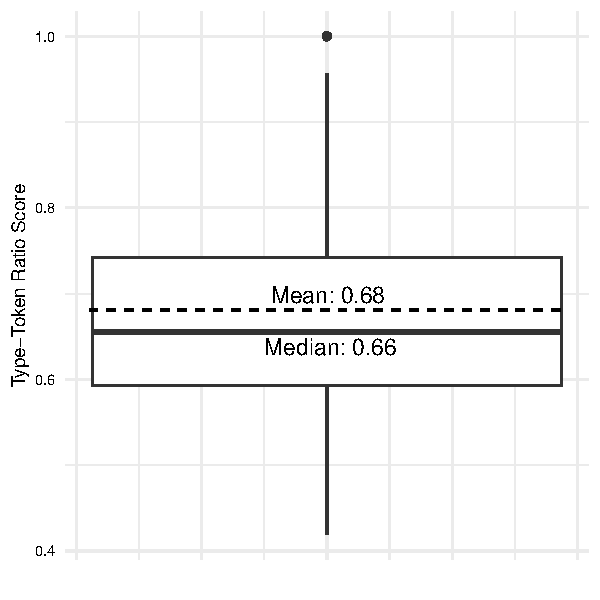
\includegraphics{approaching-analysis_files/figure-pdf/fig-aa-belc-boxplot-trimmed-1.pdf}

}

}

\subcaption{\label{fig-aa-belc-boxplot-trimmed-1}Type-token ratio score}
\end{minipage}%
%
\begin{minipage}[t]{0.50\linewidth}

{\centering 

\raisebox{-\height}{

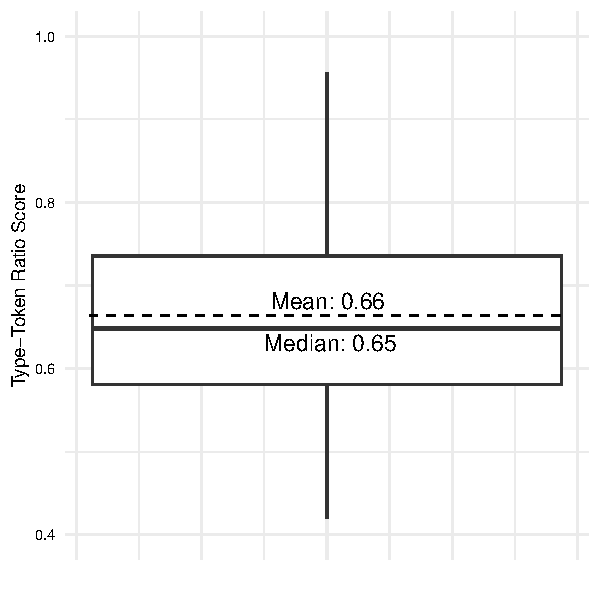
\includegraphics{approaching-analysis_files/figure-pdf/fig-aa-belc-boxplot-trimmed-2.pdf}

}

}

\subcaption{\label{fig-aa-belc-boxplot-trimmed-2}Type-token ratio score
(trimmed)}
\end{minipage}%

\caption{\label{fig-aa-belc-boxplot-trimmed}Boxplots for \texttt{ttr}
before and after trimming.}

\end{figure}

We can now appreciate the relatively larger effect that the outliers had
on the mean value of the \texttt{ttr} variable. As outliers are removed
as the difference between the mean and median will become smaller.

The exploration the data points with histograms and boxplots has helped
us to identify outliers. Now we turn to the question of the overall
shape of the distribution. The key question is whether the observed
distribution of each variable approximates the Normal Distribution, or
not.

The \textbf{Normal Distribution} is a theoretical distribution where the
values are symmetrically dispersed around the central tendency (mean/
median). In terms we can now understand, this means that the mean and
median are the same. The Normal Distribution is important because many
statistical tests assume that the data distribution is normal or near
normal.

Stepping away from our BELC dataset, I've created simulated data that
fit normal and non-normal, or skewed, distributions. I present each of
these distributions as density plots with mean and median line overlays
in Figure~\ref{fig-aa-distributions}.

\begin{figure}

\begin{minipage}[t]{0.33\linewidth}

{\centering 

\raisebox{-\height}{

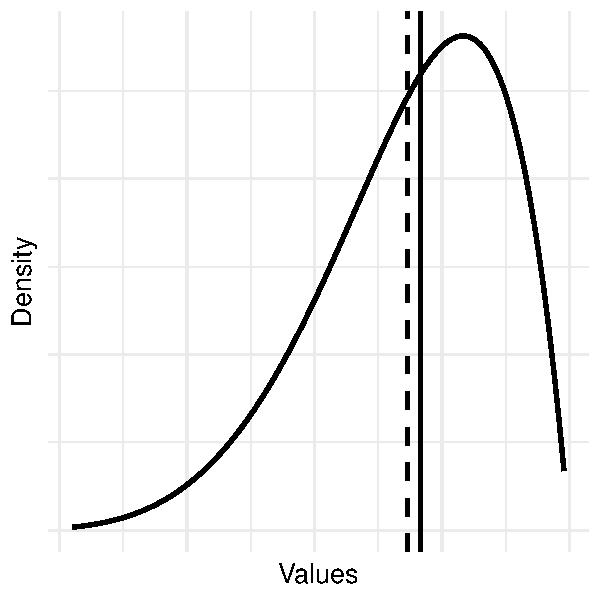
\includegraphics{approaching-analysis_files/figure-pdf/fig-aa-distributions-1.pdf}

}

}

\subcaption{\label{fig-aa-distributions-1}Left skewed distribution}
\end{minipage}%
%
\begin{minipage}[t]{0.33\linewidth}

{\centering 

\raisebox{-\height}{

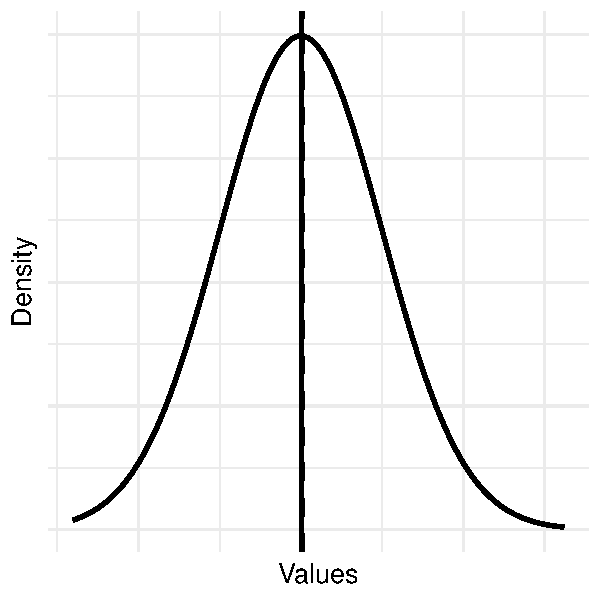
\includegraphics{approaching-analysis_files/figure-pdf/fig-aa-distributions-2.pdf}

}

}

\subcaption{\label{fig-aa-distributions-2}Normal distribution}
\end{minipage}%
%
\begin{minipage}[t]{0.33\linewidth}

{\centering 

\raisebox{-\height}{

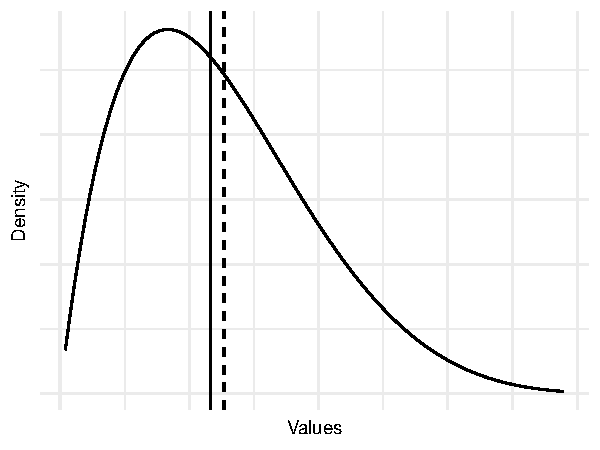
\includegraphics{approaching-analysis_files/figure-pdf/fig-aa-distributions-3.pdf}

}

}

\subcaption{\label{fig-aa-distributions-3}Right skewed distribution}
\end{minipage}%

\caption{\label{fig-aa-distributions}Mean and median for normal and
skewed distributions.}

\end{figure}

A \textbf{Normal Distribution}, illustrated in
Figure~\ref{fig-aa-distributions-2}, is a distribution where the values
are symmetrically dispersed around the central tendency (mean/ median).
This means that in a theoretical distribution that the mean and median
are the same. The Normal Distribution is also known as the
\textbf{Gaussian Distribution} or the \textbf{Bell Curve}, for the
hallmark bell shape of the distribution. In this distribution, extreme
values are less likely than values near the center.

A \textbf{skewed distribution} is not a specific type of distribution
but rather a characteristic than many distributions can exhibit where
the values are not symmetrically dispersed around the central tendency.
A distribution in which values tend to disperse to the left of the
central tendency is \textbf{left skewed} as in
Figure~\ref{fig-aa-distributions-1} and dispersion to the right is
\textbf{right skewed} as in Figure~\ref{fig-aa-distributions-3}.

Data that are normally, or near-normally distributed are often analyzed
using parametric tests while data that exhibit a skewed distributed are
often analyzed using non-parametric tests. Divergence from normality is
not a binary distinction. Rather, it is a matter of degree. A visual
inspection is usually sufficient for experienced researchers to
determine whether a distribution is normal or skewed. However, for those
who are less experienced or if you want to be more precise, there are
two primary measures which can help ascertain the degree to which a
distribution is normal: skewness and kurtosis. \textbf{Skewness} is a
measure of the degree to which a distribution is asymmetrical.
\textbf{Kurtosis} is a measure of the degree to which a distribution is
peaked.

In Table~\ref{tbl-aa-skewness-kurtosis} I provide the skewness and
kurtosis scores for our simulated distributions along with central
tendency measures for context.

\hypertarget{tbl-aa-skewness-kurtosis}{}
\begin{longtable}[]{@{}lrrlrr@{}}
\caption{\label{tbl-aa-skewness-kurtosis}Skewness and kurtosis for
normal and skewed distributions.}\tabularnewline
\toprule\noalign{}
distribution & mean & median & histogram & skewness & kurtosis \\
\midrule\noalign{}
\endfirsthead
\toprule\noalign{}
distribution & mean & median & histogram & skewness & kurtosis \\
\midrule\noalign{}
\endhead
\bottomrule\noalign{}
\endlastfoot
Left skew & 0.746 & 0.767 & ▁▂▅▇▆ & -0.711 & 3.27 \\
Normal & 0.016 & 0.009 & ▁▅▇▃▁ & 0.065 & 2.93 \\
Right skew & 0.254 & 0.233 & ▆▇▅▂▁ & 0.711 & 3.27 \\
\end{longtable}

All things distribution are matters of degree, so there are no hard and
fast rules for determining whether a distribution is normal or skewed.
However, there are some general guidelines that can be used to determine
the degree to which a distribution is normal or skewed, as shown in
Table~\ref{tbl-aa-skewness-kurtosis}.

\begin{table}

\caption{\label{tbl-aa-skewness-kurtosis}Rules of thumb for skewness and
kurtosis scores.}\begin{minipage}[t]{0.50\linewidth}
\subcaption{\label{tbl-aa-skewness}Skewness scores}

{\centering 

\begin{tabular}[t]{ll}
\toprule
Score Range & Evaluation\\
\midrule
-0.5 to 0.5 & Approximately symmetric\\
-1 to -0.5 or 0.5 to 1 & Moderately skewed\\
\textless{} -1 or \textgreater{} 1 & Highly skewed\\
\bottomrule
\end{tabular}

}

\end{minipage}%
%
\begin{minipage}[t]{0.50\linewidth}
\subcaption{\label{tbl-aa-kurtosis}Kurtosis scores}

{\centering 

\begin{tabular}[t]{ll}
\toprule
Score Range & Evaluation\\
\midrule
\textless{} 3 & Less peaked than normal\\
Equal to 3 & Normal peak\\
\textgreater{} 3 & More peaked than normal\\
\bottomrule
\end{tabular}

}

\end{minipage}%

\end{table}

\begin{tcolorbox}[enhanced jigsaw, rightrule=.15mm, leftrule=.75mm, opacityback=0, arc=.35mm, colback=white, breakable, toprule=.15mm, bottomrule=.15mm, left=2mm]

\textbf{\faIcon{medal} Dive deeper}

Another approach for visually summarizing a single numeric variable is
the Empirical Cumulative Distribution Function, or \emph{ECDF}. An ECDF
plot is a summary of the cummulative proportion of each of the values of
a numeric variable. In addition to providing insight into the
distribution of a variable, ECDF plots can be useful in determing what
proportion of the values fall above or below a certain percentage of the
data.

\end{tcolorbox}

The question is which type of distribution does each numeric variable in
the BELC dataset fit? Comparing the variables \texttt{ttr},
\texttt{types} and \texttt{prop\_l2} in
Figure~\ref{fig-aa-belc-histogram-density-trimmed} to the three
distributions in Figure~\ref{fig-aa-distributions}, we see that all
three numeric variables in the BELC dataset are skewed to some degree.

\begin{figure}

\begin{minipage}[t]{0.33\linewidth}

{\centering 

\raisebox{-\height}{

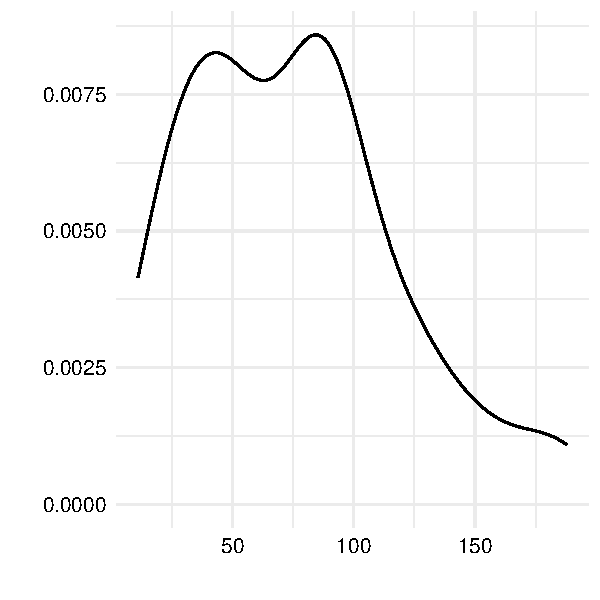
\includegraphics{approaching-analysis_files/figure-pdf/fig-aa-belc-histogram-density-trimmed-1.pdf}

}

}

\subcaption{\label{fig-aa-belc-histogram-density-trimmed-1}Type-token
ratio score}
\end{minipage}%
%
\begin{minipage}[t]{0.33\linewidth}

{\centering 

\raisebox{-\height}{

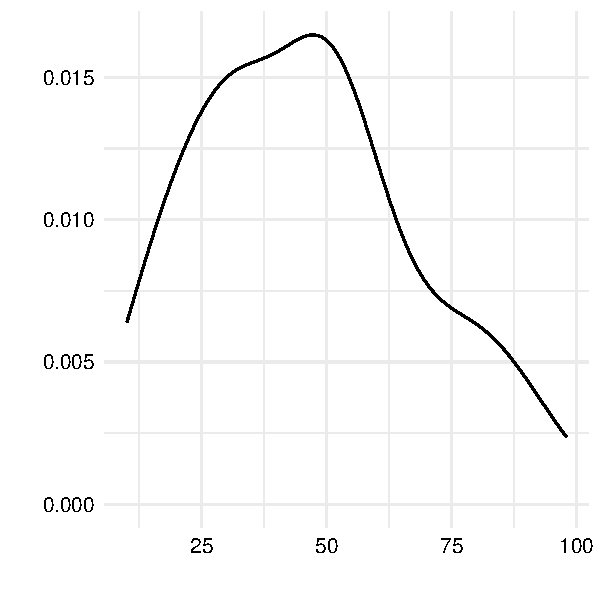
\includegraphics{approaching-analysis_files/figure-pdf/fig-aa-belc-histogram-density-trimmed-2.pdf}

}

}

\subcaption{\label{fig-aa-belc-histogram-density-trimmed-2}Number of
types}
\end{minipage}%
%
\begin{minipage}[t]{0.33\linewidth}

{\centering 

\raisebox{-\height}{

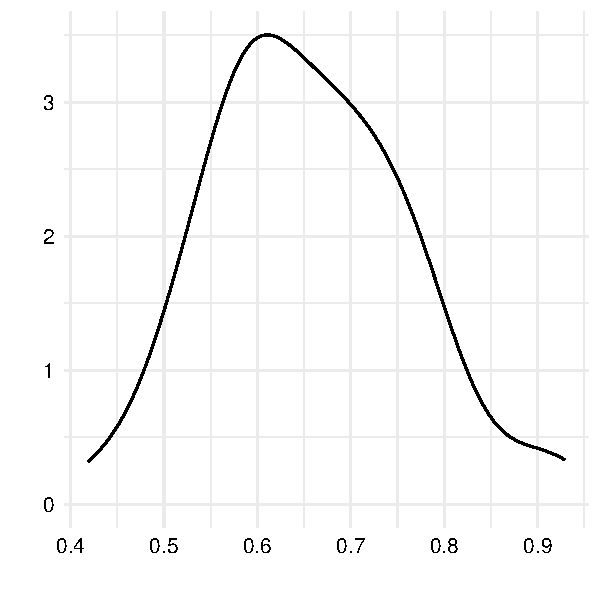
\includegraphics{approaching-analysis_files/figure-pdf/fig-aa-belc-histogram-density-trimmed-3.pdf}

}

}

\subcaption{\label{fig-aa-belc-histogram-density-trimmed-3}Proportion of
L2 words}
\end{minipage}%

\caption{\label{fig-aa-belc-histogram-density-trimmed}Histogram/ Density
plots for numeric variables in the BELC dataset.}

\end{figure}

Figure~\ref{fig-aa-belc-histogram-density-trimmed-1} for \texttt{ttr}
has some right skewing but not as much as \texttt{types} in
Figure~\ref{fig-aa-belc-histogram-density-trimmed-2}. \texttt{prop\_l2}
in Figure~\ref{fig-aa-belc-histogram-density-trimmed-3} is the most
skewed of the three variables. As mentioned earlier, skewed
distributions can take many forms, some are more skewed than others.

To view statistics on our three variables in
Figure~\ref{fig-aa-belc-histogram-density-trimmed}, we can calculate the
skewness and kurtosis.

\hypertarget{tbl-aa-belc-skewness-kurtosis}{}
\begin{longtable}[]{@{}lrrlrr@{}}
\caption{\label{tbl-aa-belc-skewness-kurtosis}Skewness and kurtosis for
numeric variables in the BELC dataset.}\tabularnewline
\toprule\noalign{}
distribution & mean & median & histogram & skewness & kurtosis \\
\midrule\noalign{}
\endfirsthead
\toprule\noalign{}
distribution & mean & median & histogram & skewness & kurtosis \\
\midrule\noalign{}
\endhead
\bottomrule\noalign{}
\endlastfoot
ttr & 0.655 & 0.648 & ▂▇▇▆▁ & 0.319 & 2.90 \\
types & 46.044 & 46.000 & ▅▇▇▃▂ & 0.407 & 2.45 \\
tokens & 75.338 & 77.000 & ▇▇▇▃▂ & 0.669 & 2.98 \\
prop\_l2 & 0.986 & 0.990 & ▁▁▂▃▇ & -1.273 & 4.13 \\
\end{longtable}

Given the characteristics of the numeric variables in the BELC dataset,
although none of them are perfectly normal, but only \texttt{prop\_l2}
is highly skewed. Therefore, if we intend to use these variables `as-is'
in statistical measures or tests, we now know whether to choose
parametric or non-parametric alternatives.

In the case that a variable is highly skewed, it is often useful to
attempt transform the variable to reduce the skewness. In contrast to
scale-based transformations (\emph{e.g.} centering and scaling),
shape-based transformations change the scale and the shape of the
distribution. The most common shape-based transformation is the
logarithmic transformation. The \textbf{logarithmic transformation}
(log-transformation) takes the log (typically base 10) of each value in
a variable. The log-transformation is useful for reducing the skewness
of a variable as it compresses large values and expands small values. If
the skewness is due to these factors, the log-transformation can help.

It is important to note, however, that if scale-based transformations
are to be applied to a variable, they should be applied after the
log-transformation as the log of negative values is undefined.

\hypertarget{interdependence}{%
\subsubsection{Interdependence}\label{interdependence}}

We have covered the first three of the four questions we are interested
in asking in a descriptive analysis. The fourth, and last, question is
whether there is mutual dependence between variables. If so, what is the
directionality and how strong is the dependence? Knowing the answers to
these questions will help frame our approach to analysis.

To assess interdependence, the number and information types of the
variables under consideration are important. Let's start by considering
two variables. If we are working with two variables, we are dealing with
a \textbf{bivariate} relationship. Given there are three informational
types (categorical, ordinal, and numeric), there are six logical
bivariate combinations: categorical-categorical, categorical-ordinal,
categorical-numeric, ordinal-ordinal, ordinal-numeric, and
numeric-numeric.

The directionality of a relationship will take the form of a tabular or
graphic summary depending on the informational value of the variables
involved. In Table~\ref{tbl-aa-summary-types}, we see the appropriate
summary types for each of the six bivariate combinations.

\hypertarget{tbl-aa-summary-types}{}
\begin{longtable}[]{@{}
  >{\raggedright\arraybackslash}p{(\columnwidth - 6\tabcolsep) * \real{0.1400}}
  >{\raggedright\arraybackslash}p{(\columnwidth - 6\tabcolsep) * \real{0.2200}}
  >{\raggedright\arraybackslash}p{(\columnwidth - 6\tabcolsep) * \real{0.3000}}
  >{\raggedright\arraybackslash}p{(\columnwidth - 6\tabcolsep) * \real{0.2200}}@{}}
\caption{\label{tbl-aa-summary-types}Appropriate summary types for
different combinations of variable types.}\tabularnewline
\toprule\noalign{}
\begin{minipage}[b]{\linewidth}\raggedright
\end{minipage} & \begin{minipage}[b]{\linewidth}\raggedright
Categorical
\end{minipage} & \begin{minipage}[b]{\linewidth}\raggedright
Ordinal
\end{minipage} & \begin{minipage}[b]{\linewidth}\raggedright
Numeric
\end{minipage} \\
\midrule\noalign{}
\endfirsthead
\toprule\noalign{}
\begin{minipage}[b]{\linewidth}\raggedright
\end{minipage} & \begin{minipage}[b]{\linewidth}\raggedright
Categorical
\end{minipage} & \begin{minipage}[b]{\linewidth}\raggedright
Ordinal
\end{minipage} & \begin{minipage}[b]{\linewidth}\raggedright
Numeric
\end{minipage} \\
\midrule\noalign{}
\endhead
\bottomrule\noalign{}
\endlastfoot
\textbf{Categorical} & Contingency table & Contingency table/ Bar plot &
Pivot table/ Boxplot \\
\textbf{Ordinal} & - & Contingency table/ Bar plot & Pivot table/
Boxplot \\
\textbf{Numeric} & - & - & Scatterplot \\
\end{longtable}

Let's first start with the combinations that include a categorical or
ordinal variable. Categorical and ordinal variables reflect measures of
class-type information, with add meaningful ranks to ordinal variables.
To assess a relationship with these variable types, a table is always a
good place to start. When combined together, a contingency table is the
appropriate table. A \textbf{contingency table} is a cross-tabulation of
two class-type variables, basically a two-way frequency table. This
means that three of the six bivariate combinations are assessed with a
contingency table: categorical-categorical, categorical-ordinal, and
ordinal-ordinal.

In Table~\ref{tbl-aa-belc-contingency-tables} we see contingency tables
for the categorical variable \texttt{sex} and ordinal variable
\texttt{group} in the BELC dataset.

\begin{table}

\caption{\label{tbl-aa-belc-contingency-tables}Contingency tables for
categorical variable \texttt{sex} and ordinal variable \texttt{group} in
the BELC dataset.}\begin{minipage}[t]{0.50\linewidth}
\subcaption{\label{tbl-aa-belc-contingency-tables-1}Counts}

{\centering 

\begin{tabular}[t]{lrrr}
\toprule
group & female & male & Total\\
\midrule
T1 & 7 & 9 & 16\\
T2 & 11 & 4 & 15\\
T3 & 13 & 10 & 23\\
T4 & 9 & 5 & 14\\
Total & 40 & 28 & 68\\
\bottomrule
\end{tabular}

}

\end{minipage}%
%
\begin{minipage}[t]{0.50\linewidth}
\subcaption{\label{tbl-aa-belc-contingency-tables-2}Percentages}

{\centering 

\begin{tabular}[t]{llll}
\toprule
group & female & male & Total\\
\midrule
T1 & 43.75\% & 56.25\% & 100.00\%\\
T2 & 73.33\% & 26.67\% & 100.00\%\\
T3 & 56.52\% & 43.48\% & 100.00\%\\
T4 & 64.29\% & 35.71\% & 100.00\%\\
Total & 58.82\% & 41.18\% & 100.00\%\\
\bottomrule
\end{tabular}

}

\end{minipage}%

\end{table}

A contingency table may include only counts, as in
Table~\ref{tbl-aa-belc-contingency-tables-1}, or may include proportions
or percentages in an effort to normalize the counts and make them more
comparable, as in Table~\ref{tbl-aa-belc-contingency-tables-2}.

It is sometimes helpful to visualize a contingency table as a bar plot
when there are a larger number of levels in either or both of the
variables. Again, looking at the relationship between \texttt{sex} and
\texttt{group}, we see that we can plot the counts or the proportions.
In Figure~\ref{fig-aa-belc-bar-plots}, we see both.

\begin{figure}

\begin{minipage}[t]{0.50\linewidth}

{\centering 

\raisebox{-\height}{

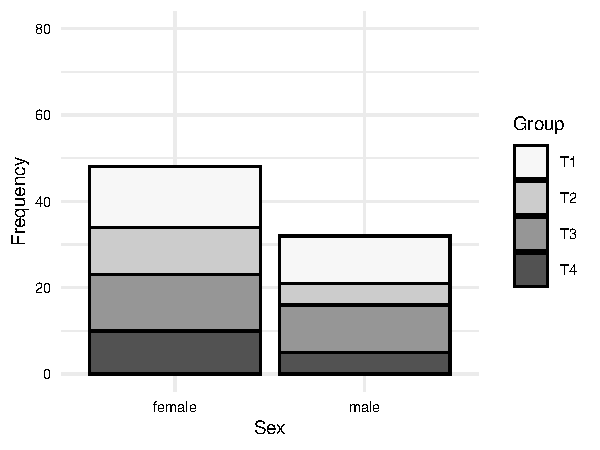
\includegraphics{approaching-analysis_files/figure-pdf/fig-aa-belc-bar-plots-1.pdf}

}

}

\subcaption{\label{fig-aa-belc-bar-plots-1}Counts}
\end{minipage}%
%
\begin{minipage}[t]{0.50\linewidth}

{\centering 

\raisebox{-\height}{

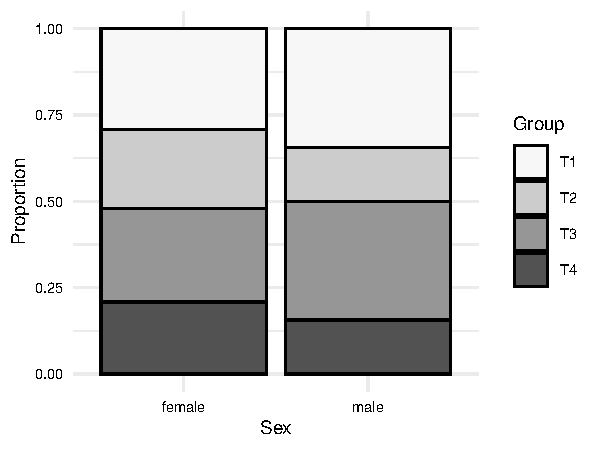
\includegraphics{approaching-analysis_files/figure-pdf/fig-aa-belc-bar-plots-2.pdf}

}

}

\subcaption{\label{fig-aa-belc-bar-plots-2}Proportions}
\end{minipage}%

\caption{\label{fig-aa-belc-bar-plots}Bar plots for the relationship
between \texttt{sex} and \texttt{group} in the BELC dataset.}

\end{figure}

To summarize and assess the relationship between a categorical or an
ordinal variable and a numeric variable, we cannot use a contingency
table. Instead, this type of relationship is best summarized in a table
using a summary statistic in a \textbf{pivot table}. A pivot table is a
table in which a class-type variable is used to group a numeric variable
by some summary statistic appropriate for numeric variables, \emph{e.g.}
mean, median, standard deviation, \emph{etc.}

In Table~\ref{tbl-aa-belc-pivot-table}, we see a pivot table for the
relationship between \texttt{group} and \texttt{tokens} in the BELC
dataset. Specifically, we see the mean number of tokens by group.

\hypertarget{tbl-aa-belc-pivot-table}{}
\begin{longtable}[]{@{}lr@{}}
\caption{\label{tbl-aa-belc-pivot-table}Pivot table for the relationship
between \texttt{group} and \texttt{tokens} in the BELC
dataset.}\tabularnewline
\toprule\noalign{}
group & mean\_tokens \\
\midrule\noalign{}
\endfirsthead
\toprule\noalign{}
group & mean\_tokens \\
\midrule\noalign{}
\endhead
\bottomrule\noalign{}
\endlastfoot
T1 & 35.4 \\
T2 & 62.5 \\
T3 & 85.0 \\
T4 & 118.9 \\
\end{longtable}

We see that the mean number of tokens increases from Group T1 to T4,
which is consistent with the idea that the students in the higher groups
are writing longer essays.

Although a pivot table may be appropriate for targeted numeric
summaries, a visualization is often more informative for assessing the
dispersion and distribution of a numeric variable by a categorical or
ordinal variable. There are two main types of visualizations for this
type of relationship: a boxplot and a \textbf{violin plot}. A violin
plot is a visualization that summarizes the distribution of a numeric
variable by a categorical or ordinal variable, adding the overall shape
of the distribution, much as a density plot does for histograms.

In Figure~\ref{fig-aa-belc-boxplot-violin-plot}, we see both a boxplot
and a violin plot for the relationship between \texttt{group} and
\texttt{tokens} in the BELC dataset.

\begin{figure}

\begin{minipage}[t]{0.50\linewidth}

{\centering 

\raisebox{-\height}{

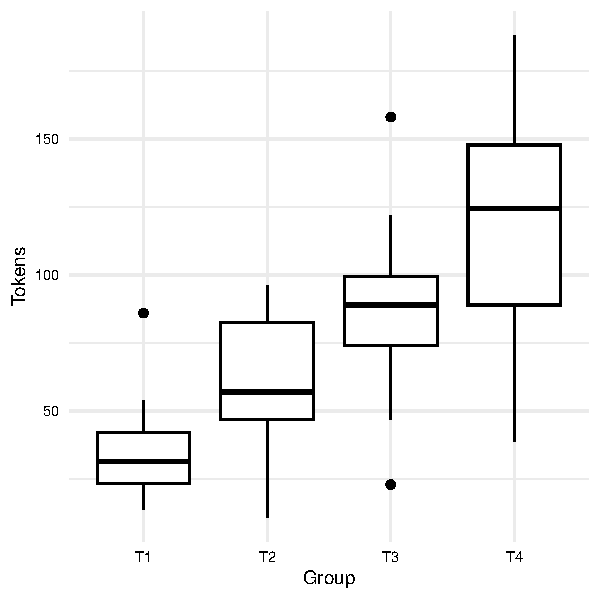
\includegraphics{approaching-analysis_files/figure-pdf/fig-aa-belc-boxplot-violin-plot-1.pdf}

}

}

\subcaption{\label{fig-aa-belc-boxplot-violin-plot-1}Boxplot}
\end{minipage}%
%
\begin{minipage}[t]{0.50\linewidth}

{\centering 

\raisebox{-\height}{

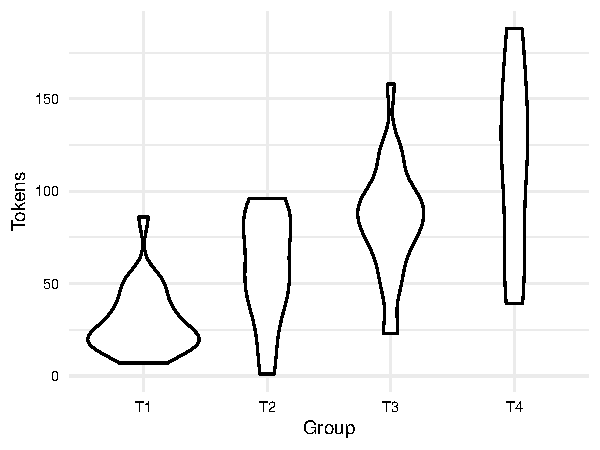
\includegraphics{approaching-analysis_files/figure-pdf/fig-aa-belc-boxplot-violin-plot-2.pdf}

}

}

\subcaption{\label{fig-aa-belc-boxplot-violin-plot-2}Violin plot}
\end{minipage}%

\caption{\label{fig-aa-belc-boxplot-violin-plot}Boxplot and violin plot
for the relationship between \texttt{group} and \texttt{tokens} in the
BELC dataset.}

\end{figure}

From the boxplot in Figure~\ref{fig-aa-belc-boxplot-violin-plot-1}, we
see that the general trend towards more tokens used by students in
higher groups. But we can also appreciate the dispersion of the data
within each group looking at the boxes and whiskers. On the surface it
appears that the data for groups T1 and T3 are closer to each other than
groups T2 and T4, in which there is more variability within these
groups. Furthermore, we can see outliers in groups T1 and T3, but not in
groups T2 and T4. From the violin plot in
Figure~\ref{fig-aa-belc-boxplot-violin-plot-2}, we can see the same
information, but we can also see the overall shape of the distribution
of tokens within each group. In this plot, it is very clear that group
T4 includes a wide range of token counts.

The last bivariate combination is numeric-numeric. To summarize this
type of relationship a scatterplot is used. A \textbf{scatterplot} is a
visualization that plots each data point as a point in a two-dimensional
space, with one numeric variable on the x-axis and the other numeric
variable on the y-axis. Depending on the type of relationship you are
trying to assess, you may want to add a trend line to the scatterplot. A
trend line is a line that summarizes the overall trend in the
relationship between the two numeric variables. To assess the extent to
which the relationship is linear, a straight line is drawn which
minimizes the distance between the line and the points.

In Figure~\ref{fig-aa-belc-scatter-plot}, we see a scatterplot and a
scatterplot with a trend line for the relationship between \texttt{ttr}
and \texttt{types} in the BELC dataset.

\begin{figure}

\begin{minipage}[t]{0.50\linewidth}

{\centering 

\raisebox{-\height}{

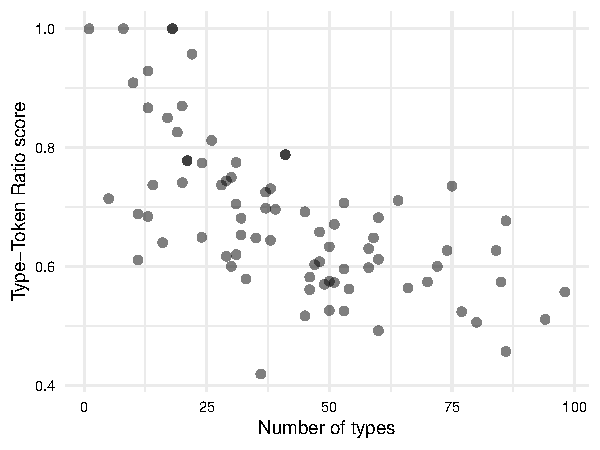
\includegraphics{approaching-analysis_files/figure-pdf/fig-aa-belc-scatter-plot-1.pdf}

}

}

\subcaption{\label{fig-aa-belc-scatter-plot-1}Points}
\end{minipage}%
%
\begin{minipage}[t]{0.50\linewidth}

{\centering 

\raisebox{-\height}{

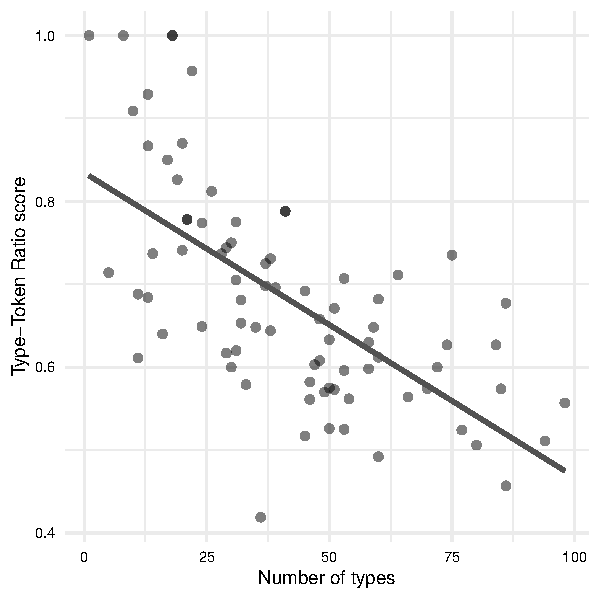
\includegraphics{approaching-analysis_files/figure-pdf/fig-aa-belc-scatter-plot-2.pdf}

}

}

\subcaption{\label{fig-aa-belc-scatter-plot-2}Points with a linear trend
line}
\end{minipage}%

\caption{\label{fig-aa-belc-scatter-plot}Scatter plot for the
relationship between \texttt{ttr} and \texttt{types} in the BELC
dataset.}

\end{figure}

We see that there is an apparent positive relationship between these two
variables, which is consistent with the idea that as the number of types
increases, the type-token ratio increases. In other words, as the number
of unique words increases, so does the lexical diversity of the text.
Since we are evaluating a linear relationship, we are assessing the
extent to which there is a \textbf{correlation} between \texttt{ttr} and
\texttt{types}. A correlation simply means that as the values of one
variable change, the values of the other variable change in a consistent
manner.

Once a sense of the directionality of a relationship can be established,
the next step is to gauge the relative strength, or association.
\textbf{Association} refers to any relationship in which there is a
dependency between two variables. Quantitative measures of association,
in combination with tabular and visual summaries, can provide a more
complete picture of the relationship between two variables.

There are a number of measures of assocation, depending on the types of
variables being assessed and, for numeric variables, whether the
distribution is normal (parametric) or non-normal (non-parametric), as
seen in Table~\ref{tbl-aa-association-measures}.

\hypertarget{tbl-aa-association-measures}{}
\begin{longtable}[]{@{}
  >{\raggedright\arraybackslash}p{(\columnwidth - 8\tabcolsep) * \real{0.2000}}
  >{\raggedright\arraybackslash}p{(\columnwidth - 8\tabcolsep) * \real{0.2000}}
  >{\raggedright\arraybackslash}p{(\columnwidth - 8\tabcolsep) * \real{0.2000}}
  >{\raggedright\arraybackslash}p{(\columnwidth - 8\tabcolsep) * \real{0.2000}}
  >{\raggedright\arraybackslash}p{(\columnwidth - 8\tabcolsep) * \real{0.2000}}@{}}
\caption{\label{tbl-aa-association-measures}Measures of association or
correlation strength for different combinations of variable
types.}\tabularnewline
\toprule\noalign{}
\begin{minipage}[b]{\linewidth}\raggedright
\end{minipage} & \begin{minipage}[b]{\linewidth}\raggedright
Categorical
\end{minipage} & \begin{minipage}[b]{\linewidth}\raggedright
Ordinal
\end{minipage} & \begin{minipage}[b]{\linewidth}\raggedright
Numeric\emph{Non-parametric}
\end{minipage} & \begin{minipage}[b]{\linewidth}\raggedright
Numeric\emph{Parametric}
\end{minipage} \\
\midrule\noalign{}
\endfirsthead
\toprule\noalign{}
\begin{minipage}[b]{\linewidth}\raggedright
\end{minipage} & \begin{minipage}[b]{\linewidth}\raggedright
Categorical
\end{minipage} & \begin{minipage}[b]{\linewidth}\raggedright
Ordinal
\end{minipage} & \begin{minipage}[b]{\linewidth}\raggedright
Numeric\emph{Non-parametric}
\end{minipage} & \begin{minipage}[b]{\linewidth}\raggedright
Numeric\emph{Parametric}
\end{minipage} \\
\midrule\noalign{}
\endhead
\bottomrule\noalign{}
\endlastfoot
\textbf{Categorical} & Chi-square \(\chi^2\), Cramér's \(V\) & Goodman
and Kruskal's \(\gamma\) & Rank biserial Correlation & Point-biseral
Correlation \\
\textbf{Ordinal} & - & Kendall's \(\tau\) & Kendall's \(\tau\) &
Pearson's \(r\) \\
\textbf{Numeric}\emph{Non-parametric} & - & - & Kendall's \(\tau\) &
Pearson's \(r\) \\
\textbf{Numeric}\emph{Parametric} & - & - & - & Pearson's \(r\) \\
\end{longtable}

Association measures often are expressed as a number between -1 and 1,
where 0 indicates no association, -1 indicates a perfect negative
association, and 1 indicates a perfect positive association. The closer
the number is to 0, the weaker the association. The closer the number is
to -1 or 1, the stronger the association. Association statistics are
often accompanied by a \textbf{confidence interval} (CI), which is a
range of values that is likely to contain the true value of the
association in the population. The confidence interval is expressed as a
percentage, such as 95\%, which means that if we were to repeat the
study 100 times, 95 of those studies would produce a confidence interval
that contains the true value of the association in the population. If
the range between the lower and higher bounds of the confidence interval
contains 0, then the association is likely no different than chance.

Given these measures and interpretations, let's consider the different
types of bivariate relationships we have seen so far in the BELC
dataset. The first interdependence we explored involved the categorical
variable \texttt{sex} and the ordinal variable \texttt{group}. This
relationship may not be of primary interest to a study on L2 writing,
but it is a good example of how to assess the strength of an association
between a categorical and ordinal variable. Furthermore, it could be the
case that we want to assess whether we have widely unbalanced female/
male proportions in our time groups.

Using Table~\ref{tbl-aa-association-measures}, we see that we can use
Goodman and Kruskal's \(\gamma\) (gamma) to assess the strength of the
association between these two variables. The measures of association in
Table~\ref{tbl-aa-gamma} suggest that the proportion of male
participants is higher in group T1 and lower in group T2. However, these
associations are moderately strong, as the gamma value is near \(\pm\)
0.4.

\hypertarget{tbl-aa-gamma}{}
\begin{longtable}[]{@{}llrrrr@{}}
\caption{\label{tbl-aa-gamma}Gamma for the relationship between
\texttt{sex} and \texttt{group} in the BELC dataset.}\tabularnewline
\toprule\noalign{}
Parameter1 & Parameter2 & r & CI & CI\_low & CI\_high \\
\midrule\noalign{}
\endfirsthead
\toprule\noalign{}
Parameter1 & Parameter2 & r & CI & CI\_low & CI\_high \\
\midrule\noalign{}
\endhead
\bottomrule\noalign{}
\endlastfoot
sex.female & group.T1 & -0.381 & 0.95 & -0.568 & -0.157 \\
sex.female & group.T2 & 0.389 & 0.95 & 0.167 & 0.575 \\
sex.male & group.T1 & 0.381 & 0.95 & 0.157 & 0.568 \\
sex.male & group.T2 & -0.389 & 0.95 & -0.575 & -0.167 \\
\end{longtable}

When paired with Figure~\ref{fig-aa-belc-bar-plots} we can appreciate
that groups T1 and T2 have contrasting proportions of females to males
and that groups T3 and T4 are more closely proportioned. This
observation should be considered when approaching statistical analyses
in which categorical variables required (near) equal proportions of
categories.

Now let's take a look at a more interesting relationship, the one
between the ordinal variable \texttt{group} and the numeric variable
\texttt{tokens}. Since we determined that \texttt{tokens} was near
normally distributed, we can choose the parametric version of our
association measure, Pearson's \(r\). The measures of association in
Table~\ref{tbl-aa-pearson} suggest that there is a negative association
between group T1 and a positive one betwen group T4 and \texttt{tokens},
which is consistent with the idea that as the group number increases,
the number of tokens increases. These associations are moderate to
strong, as the Pearson's \(r\) values are near \(\pm\) 0.5. However, the
other groups (T2 and T3) have very weak assocations with \texttt{tokens}
and the CI includes 0, which means that the association is likely no
different than chance.

\hypertarget{tbl-aa-pearson}{}
\begin{longtable}[]{@{}llrrrr@{}}
\caption{\label{tbl-aa-pearson}Pearson's r for the relationship between
\texttt{group} and \texttt{tokens} in the BELC dataset.}\tabularnewline
\toprule\noalign{}
Parameter1 & Parameter2 & r & CI & CI\_low & CI\_high \\
\midrule\noalign{}
\endfirsthead
\toprule\noalign{}
Parameter1 & Parameter2 & r & CI & CI\_low & CI\_high \\
\midrule\noalign{}
\endhead
\bottomrule\noalign{}
\endlastfoot
group.T1 & tokens & -0.520 & 0.95 & -0.675 & -0.322 \\
group.T2 & tokens & -0.160 & 0.95 & -0.384 & 0.082 \\
group.T3 & tokens & 0.161 & 0.95 & -0.080 & 0.385 \\
group.T4 & tokens & 0.521 & 0.95 & 0.322 & 0.675 \\
\end{longtable}

These association measures suggest that there is a relationship between
\texttt{group} and \texttt{tokens}, but that the relationship is not the
same for all groups. This may due to a number of factors, such as the
number of participants in each group, the effect of outliers within
particular levels, etc. or may simply underscore that the relationship
between \texttt{group} and \texttt{tokens} is not linear. What we do
with this information will depend on our research aims. Whatever the
case, we can use these measures to inform our next steps, as we will see
in the next section.

Finally, let's look at the relationship between the numeric variables
\texttt{ttr} and \texttt{types}. Since we determined both \texttt{ttr}
and \texttt{types} are normally distributed, we can choose the
parametric version of our association measure, Pearson's \(r\). The
measures of association in Table~\ref{tbl-aa-pearson-2} suggest that
there is a negative association between \texttt{ttr} and \texttt{types},
which is consistent with the idea that as the number of types increases,
the type-token ratio decreases. This association is strong, as Pearson's
\(r\) value is near 0.6.

\hypertarget{tbl-aa-pearson-2}{}
\begin{longtable}[]{@{}llrrrr@{}}
\caption{\label{tbl-aa-pearson-2}Pearson's r for the relationship
between \texttt{ttr} and \texttt{types} in the BELC
dataset.}\tabularnewline
\toprule\noalign{}
Parameter1 & Parameter2 & r & CI & CI\_low & CI\_high \\
\midrule\noalign{}
\endfirsthead
\toprule\noalign{}
Parameter1 & Parameter2 & r & CI & CI\_low & CI\_high \\
\midrule\noalign{}
\endhead
\bottomrule\noalign{}
\endlastfoot
ttr & types & -0.606 & 0.95 & -0.738 & -0.43 \\
\end{longtable}

Before moving on to the next section, it is important to remember than
through the process of diagnostic measures, we gain a thorough
understanding of our data's characteristics and quality, preparing us
for the next step in our analysis. However, remember that these measures
do not exist in isolation. The decisions we make at this stage, from
handling missing data to understanding the distribution of our
variables, can have significant implications on our subsequent analysis.
So, this initial step of data analysis deserves our careful attention
and scrutiny.

\hypertarget{sec-aa-analyze}{%
\section{Analyze}\label{sec-aa-analyze}}

Having ensured that our dataset is clean, valid, and thoroughly
understood, we can proceed to the next key stage of our data analysis
process - employing analytic methods. The goal of analysis, generally,
is to generate knowledge from information. The type of knowledge
generated and the process by which it is generated, however, differ and
can be broadly grouped into three analysis types: exploratory,
predictive, and inferential.

In this section I will provide an overview of how each of these analysis
types are tied to research aims and how the general purpose of each type
affect: (1) how to \emph{identify} the variables of interest, (2) how to
\emph{interrogate} these variables, and (3) how to \emph{interpret} the
results. I will structure the discussion of these analysis types moving
from the least structured (inductive) to most structured (deductive)
approach to deriving knowledge from information with the aim to provide
enough information for you to identify these research approaches in the
literature and to make appropriate decisions as to which approach your
research should adopt.

\hypertarget{sec-aa-explore}{%
\subsection{Explore}\label{sec-aa-explore}}

In \textbf{Exploratory Data Analysis (EDA)}, we use a variety of methods
to identify patterns, trends, and relations within and between
variables. The goal of EDA is uncover insights in an inductive,
data-driven manner. That is to say, that we do not enter into EDA with a
fixed hypothesis in mind, but rather we explore intuition, probe
anecdote, and follow hunches to identify patterns and relationships and
to evaluate whether and why they are meaningful. We are admittedly
treading new or unfamiliar terrain letting the data guide our analysis.
This means that we can use and reuse the same data to explore different
angles and approaches adjusting our methods and measures as we go. In
this way, EDA is an iterative, meaning generating process.

In line with the investigative nature of EDA, the identification of
variables of interest is a discovery process. We most likely have a
intution about the variables we would like to explore, but we are able
to adjust our variables as need be to suit our research aims. When the
identification and selection of variables is open, the process is known
as \textbf{feature engineering}. A process that is much an art as a
science, feature engineering leverages a mixture of relevant domain
knowledge, intuition, and trial and error to identify features that
serve to best represent the data and to best serve the research aims.
Furthermore, the roles of features in EDA are fluid --no variable has a
special status, as seen in Figure~\ref{fig-eda-variables}. We will see
that in other types of analysis, some or all the roles of the variables
are fixed.

\begin{figure}[H]

{\centering 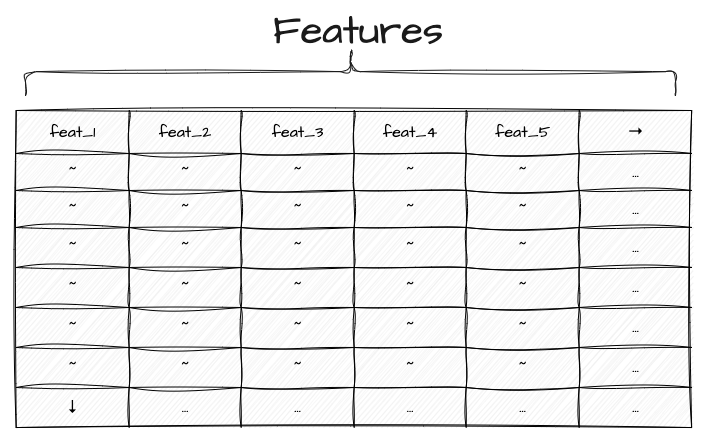
\includegraphics[width=0.5\textwidth,height=\textheight]{figures/approaching-analysis/aa-eda-variables.drawio.png}

}

\caption{\label{fig-eda-variables}Roles of variables in EDA.}

\end{figure}

For illustrative purposes let's consider the State of the Union Corpus
(SOTU) (\protect\hyperlink{ref-R-quanteda.corpora}{Benoit 2020}). The
presidential addresses and a set of metadata variables are included in
the corpus. I've subsetted this corpus to only include U.S. presidents
since 1946. A tabular preview of the first 10 addresses (truncated for
display) can be found in Table~\ref{tbl-eda-sotu-corpus}.

\hypertarget{tbl-eda-sotu-corpus}{}
\begin{longtable}[]{@{}
  >{\raggedright\arraybackslash}p{(\columnwidth - 8\tabcolsep) * \real{0.1183}}
  >{\raggedright\arraybackslash}p{(\columnwidth - 8\tabcolsep) * \real{0.1183}}
  >{\raggedright\arraybackslash}p{(\columnwidth - 8\tabcolsep) * \real{0.0968}}
  >{\raggedright\arraybackslash}p{(\columnwidth - 8\tabcolsep) * \real{0.1183}}
  >{\raggedright\arraybackslash}p{(\columnwidth - 8\tabcolsep) * \real{0.5484}}@{}}
\caption{\label{tbl-eda-sotu-corpus}First ten addresses from the SOTU
Corpus.}\tabularnewline
\toprule\noalign{}
\begin{minipage}[b]{\linewidth}\raggedright
president
\end{minipage} & \begin{minipage}[b]{\linewidth}\raggedright
date
\end{minipage} & \begin{minipage}[b]{\linewidth}\raggedright
delivery
\end{minipage} & \begin{minipage}[b]{\linewidth}\raggedright
party
\end{minipage} & \begin{minipage}[b]{\linewidth}\raggedright
addresses
\end{minipage} \\
\midrule\noalign{}
\endfirsthead
\toprule\noalign{}
\begin{minipage}[b]{\linewidth}\raggedright
president
\end{minipage} & \begin{minipage}[b]{\linewidth}\raggedright
date
\end{minipage} & \begin{minipage}[b]{\linewidth}\raggedright
delivery
\end{minipage} & \begin{minipage}[b]{\linewidth}\raggedright
party
\end{minipage} & \begin{minipage}[b]{\linewidth}\raggedright
addresses
\end{minipage} \\
\midrule\noalign{}
\endhead
\bottomrule\noalign{}
\endlastfoot
Truman & 1946-01-21 & written & Democratic & To the Congress of the
United States: A quarter\ldots{} \\
Truman & 1947-01-06 & spoken & Democratic & Mr.~President, Mr.~Speaker,
Members of the Cong\ldots{} \\
Truman & 1948-01-07 & spoken & Democratic & Mr.~President, Mr.~Speaker,
and Members of the \ldots{} \\
Truman & 1949-01-05 & spoken & Democratic & Mr.~President, Mr.~Speaker,
Members of the Cong\ldots{} \\
Truman & 1950-01-04 & spoken & Democratic & Mr.~President, Mr.~Speaker,
Members of the Cong\ldots{} \\
Truman & 1951-01-08 & spoken & Democratic & Mr.~President, Mr.~Speaker,
Members of the Cong\ldots{} \\
Truman & 1952-01-09 & spoken & Democratic & Mr.~President, Mr.~Speaker,
Members of the Cong\ldots{} \\
Truman & 1953-01-07 & written & Democratic & To the Congress of the
United States: I have th\ldots{} \\
Eisenhower & 1953-02-02 & spoken & Republican & Mr.~President,
Mr.~Speaker, Members of the Eigh\ldots{} \\
Eisenhower & 1954-01-07 & spoken & Republican & Mr.~President,
Mr.~Speaker, Members of the Eigh\ldots{} \\
\end{longtable}

A dataset such as this one could serve as a starting point to explore
many different types of research questions. In order to maintain
research coherence so our efforts to not careen into a free-for-all, we
need to tether our feature engineering to a unit of analysis that is
relevant to the research question. A \textbf{unit of analysis} is the
entity that we are interested in studying. Not to be confused with the
unit of observation, which is the entity that we are able to observe and
measure.

To demonstrate the distinction, let's look consider different approaches
to analyzing the SOTU dataset. For example, the unit of analysis could
be the language of particular presidents, party ideology, or political
rhetoric in general and the unit of observation could be individual
words, phrases, sentences, etc. In some cases the unit of analysis and
the unit of observation are the same. For example, if we were interested
in potential changes use of the word ``terrorist'' over time in SOTU
addresses, the unit of analysis and the unit of observation would be the
same --individual addresses. So, depending on the perspective we are
interested in investigating, the choice of how to approach engineering
features to gain insight will vary.

By the same token, approaches for interrogating the dataset can differ
significantly, between research projects and within the same project,
but for instructive purposes, let's draw a distinction between
descriptive methods and unsupervised learning methods, as seen in
Table~\ref{tbl-eda-methods}.

\hypertarget{tbl-eda-methods}{}
\begin{longtable}[]{@{}ll@{}}
\caption{\label{tbl-eda-methods}Some common EDA methods}\tabularnewline
\toprule\noalign{}
Descriptive methods & Unsupervised learning methods \\
\midrule\noalign{}
\endfirsthead
\toprule\noalign{}
Descriptive methods & Unsupervised learning methods \\
\midrule\noalign{}
\endhead
\bottomrule\noalign{}
\endlastfoot
Frequency analysis & Cluster analysis \\
Keyness analysis & Topic Modeling \\
Co-occurence analysis & Vector Space Models \\
\end{longtable}

The first group, \textbf{descriptive methods} can be seen as a (more
robust) extenstion of the descriptive statistics covered earlier in this
chapter including statistic, tabular, and visual techniques. For
example, a frequency analysis of the SOTU dataset could be used to
identify the most common words used by U.S. political parties in their
addresses, in Figure~\ref{fig-aa-eda-sotu-descriptive-1}, or a
co-occurence analysis could be used to identify the most common words
the appear after the term ``free'', in
Figure~\ref{fig-aa-eda-sotu-descriptive-2}, in the dataset.

\begin{figure}

\begin{minipage}[t]{0.50\linewidth}

{\centering 

\raisebox{-\height}{

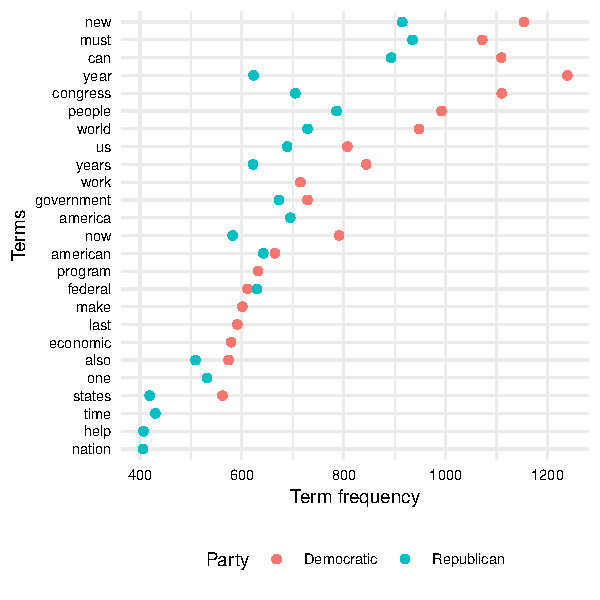
\includegraphics{approaching-analysis_files/figure-pdf/fig-aa-eda-sotu-descriptive-1.pdf}

}

}

\subcaption{\label{fig-aa-eda-sotu-descriptive-1}Frequency analysis of
the 20 most frequent terms by party.}
\end{minipage}%
%
\begin{minipage}[t]{0.50\linewidth}

{\centering 

\raisebox{-\height}{

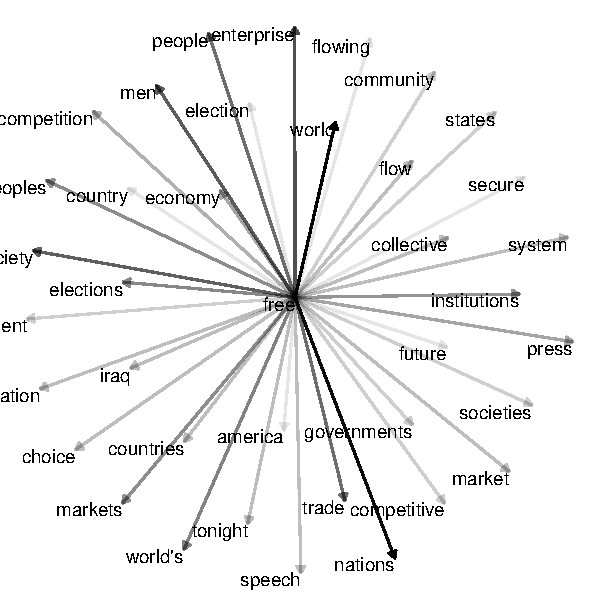
\includegraphics{approaching-analysis_files/figure-pdf/fig-aa-eda-sotu-descriptive-2.pdf}

}

}

\subcaption{\label{fig-aa-eda-sotu-descriptive-2}Co-occurence analysis
of the terms that appear after the term `free'.}
\end{minipage}%

\caption{\label{fig-aa-eda-sotu-descriptive}Example of descriptive
methods applied to the SOTU dataset.}

\end{figure}

The second group, \textbf{unsupervised learning} is a subtype of machine
learning in which an algorithm is used to find patterns within and
between variables in the data without any guidance (supervision). In
this way, the algorithm, or machine learner, is left to make connections
and associations wherever they may appear in the input data. If we were
interested in finding word-use continuities and discontinuities between
presidents, we could use a clustering algorithm, seen in
Figure~\ref{fig-aa-eda-sotu-unsupervised-1}. Or if we wanted to uncover
themes \ldots{} \faIcon{wrench} {[}ADD: modify plot{]} we could use a
vector space model, as in Figure~\ref{fig-aa-eda-sotu-unsupervised-2}.

\begin{figure}

\begin{minipage}[t]{0.50\linewidth}

{\centering 

\raisebox{-\height}{

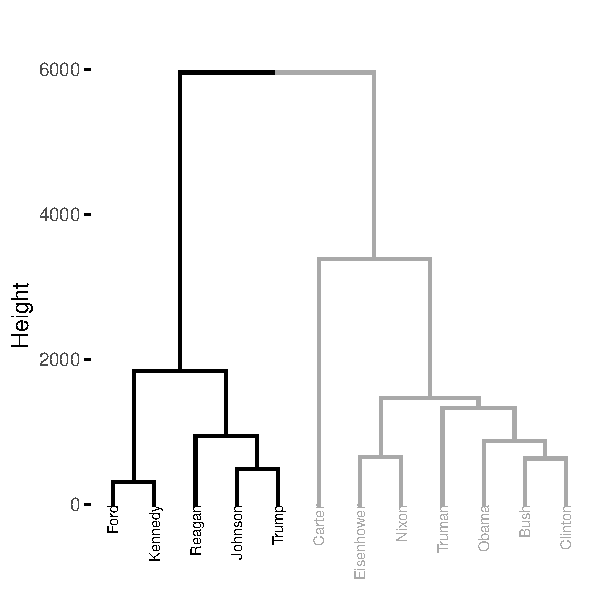
\includegraphics{approaching-analysis_files/figure-pdf/fig-aa-eda-sotu-unsupervised-1.pdf}

}

}

\subcaption{\label{fig-aa-eda-sotu-unsupervised-1}Hierarchical
clustering of the SOTU corpus.}
\end{minipage}%
%
\begin{minipage}[t]{0.50\linewidth}

{\centering 

\raisebox{-\height}{

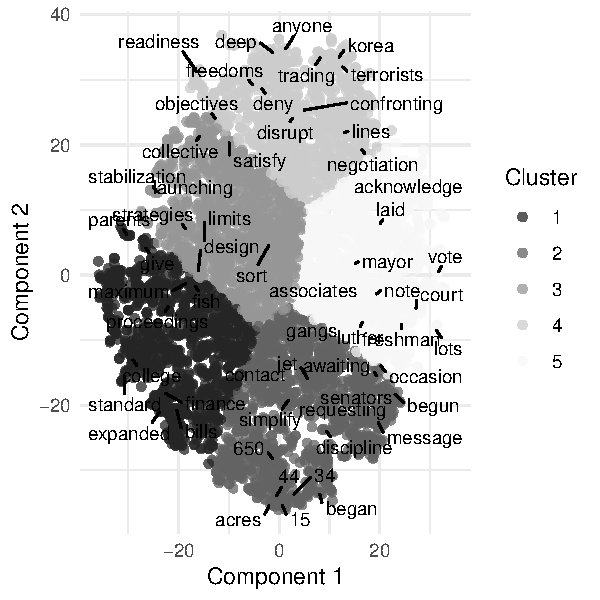
\includegraphics{approaching-analysis_files/figure-pdf/fig-aa-eda-sotu-unsupervised-2.pdf}

}

}

\subcaption{\label{fig-aa-eda-sotu-unsupervised-2}Word embedding space
in the SOTU corpus.}
\end{minipage}%

\caption{\label{fig-aa-eda-sotu-unsupervised}Example of unsupervised
learning methods applied to the SOTU dataset.}

\end{figure}

Either through descriptive, unsupervised learning methods, or a
combination of both, EDA employs quantitative methods to summarize,
reduce, and sort complex datasets in order to provide the researcher
novel perspective to be qualitatively assessed. Exploratory methods
produce results that require associative thinking and pattern detection.
Speculative as they are, the results from exploratory methods can be
highly informative and lead to new insight and inspire further study in
directions that may not have been expected.

\hypertarget{sec-aa-predict}{%
\subsection{Predict}\label{sec-aa-predict}}

\textbf{Predictive Data Analysis (PDA)} employs a variety of techniques
to examine and evaluate the association strength between a variable or
set of variables, with a specific focus on predicting a target variable.
The aim of PDA is to construct models that can accurately forecast
future outcomes, using either data-driven or theory-driven approaches.
In this process, \textbf{supervised learning} methods, where the machine
learning algorithm is guided (supervised) by a target outcome variable,
are used. This means we don't begin PDA with a completely open-ended
exploration, but rather with an objective - accurate predictions.
However, the path to achieving this objective can be flexible, allowing
us freedom to adjust our models and methods. Unlike EDA, where the
entire dataset can be reused for different approaches, PDA requires a
portion of the data to be reserved for evaluation, enhancing the
validity of our predictive models. Thus, PDA is an iterative process
that combines the flexibility of exploratory analysis with the rigor of
confirmatory analysis.

There are two types of variables in PDA: the outcome variable and the
predictor variables, or features. The \textbf{outcome variable} is the
variable that the researcher is trying to predict. It is the only
variable that is necessarily fixed as part of the research question. The
features are the variables that are used to predict the outcome
variable. An overview of the roles of these variables in PDA is shown in
Figure~\ref{fig-pda-variables}.

\begin{figure}[H]

{\centering 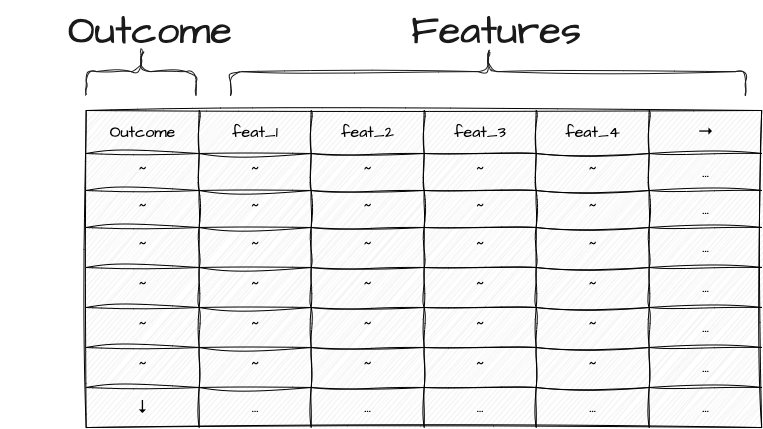
\includegraphics[width=0.5\textwidth,height=\textheight]{figures/approaching-analysis/aa-pda-variables.drawio.png}

}

\caption{\label{fig-pda-variables}Roles of variables in PDA.}

\end{figure}

Feature selection can be either data-driven or theory-driven.
Data-driven features are those that are engineered to enhance predictive
power, while theory-driven features are those that are selected based on
theoretical relevance.

Let's consider the Europarl corpus of native, non-native and translated
texts (ENNTT) (\protect\hyperlink{ref-Nisioi2016}{Nisioi et al. 23-28,
2016-05}). This is a monolingual English corpus of translated and
non-translated texts from the European Parliament.

\hypertarget{tbl-enntt-dd}{}
\begin{longtable}[]{@{}
  >{\raggedright\arraybackslash}p{(\columnwidth - 6\tabcolsep) * \real{0.1327}}
  >{\raggedright\arraybackslash}p{(\columnwidth - 6\tabcolsep) * \real{0.1947}}
  >{\raggedright\arraybackslash}p{(\columnwidth - 6\tabcolsep) * \real{0.1239}}
  >{\raggedright\arraybackslash}p{(\columnwidth - 6\tabcolsep) * \real{0.5487}}@{}}
\caption{\label{tbl-enntt-dd}Data dictionary of the ENNTT
corpus.}\tabularnewline
\toprule\noalign{}
\begin{minipage}[b]{\linewidth}\raggedright
variable
\end{minipage} & \begin{minipage}[b]{\linewidth}\raggedright
name
\end{minipage} & \begin{minipage}[b]{\linewidth}\raggedright
variable\_type
\end{minipage} & \begin{minipage}[b]{\linewidth}\raggedright
description
\end{minipage} \\
\midrule\noalign{}
\endfirsthead
\toprule\noalign{}
\begin{minipage}[b]{\linewidth}\raggedright
variable
\end{minipage} & \begin{minipage}[b]{\linewidth}\raggedright
name
\end{minipage} & \begin{minipage}[b]{\linewidth}\raggedright
variable\_type
\end{minipage} & \begin{minipage}[b]{\linewidth}\raggedright
description
\end{minipage} \\
\midrule\noalign{}
\endhead
\bottomrule\noalign{}
\endlastfoot
session\_id & Session ID & categorical & Unique identifier for each
session \\
seq\_speaker\_id & Sequential Speaker ID & ordinal & Unique numeric
identifier for each speaker \\
state & State & categorical & Country of the session speaker \\
language & Language & categorical & Original language in which the
sentence was uttered \\
type & Type & categorical & Category of the speaker: natives,
nonnatives, or translations \\
text & Text & categorical & Text spoken in the session \\
\end{longtable}

Now depending on our research question, we will have a different outcome
variable. If we want to examine the potential linguistic differences
between native and non-native speakers, we will select our outcome
variable to be the \texttt{type} (natives/ nonnatives). The features
selected to use to predict \texttt{type} depend on our research
question. If our research is guided by data, we will choose features
that are specifically designed to boost the ability to predict. On the
other hand, if our research is steered by theory, we will opt for
features that are chosen due to their theoretical significance. In
either case, the original dataset will likely need to be transformed.

The approach to interrogating the dataset includes three main steps:
feature engineering, model selection, and model evaluation. We've
discussed feature engineering, so what is model selection and model
evaluation? And how do we go about performing these steps?

\textbf{Model selection} is the process of choosing a machine learning
algorithm and set of features that produces the best prediction accuracy
for the outcome variable. To refine our approach such that we arrive at
the best combination of algorithm and features, we need to train our
machine learner on a variety of combinations and evaluate the accuracy
of each. We don't want to train and evaluate on the same data, as this
would be cheating, and likely would not produce a model that generalizes
well to new data. Instead, we split our data into two sets: a training
set and a test set. The \textbf{training set} is used to train the
machine learner, while the \textbf{test set} is used to evaluate the
accuracy of the model\footnote{Depending on the application and the
  amount of available data, a third \emph{development set} is sometimes
  created as a pseudo test set to facilitate the testing of multiple
  approaches on data outside the training set before the final
  evaluation on the test set is performed.}. The larger portion of the
data, from 60\% to 80\%, is used for training, while the remaining
portion is used for testing.

The elephant in the room is, what type of machine learning algorithm do
I use? Well, there are many different types of machine learning
algorithms, each with their own strengths and weaknesses. The first
rough cut is to decide what type of outcome variable we are predicting:
categorical or numeric. If the outcome variable is categorical, we are
performing a \textbf{classification} task, and if the outcome variable
is numeric, we are performing a \textbf{regression} task. As we see in
Table~\ref{tbl-pda-algorithms}, there are various algorithms that can be
used for each task.

\hypertarget{tbl-pda-algorithms}{}
\begin{longtable}[]{@{}
  >{\raggedright\arraybackslash}p{(\columnwidth - 4\tabcolsep) * \real{0.3300}}
  >{\raggedright\arraybackslash}p{(\columnwidth - 4\tabcolsep) * \real{0.3300}}
  >{\raggedright\arraybackslash}p{(\columnwidth - 4\tabcolsep) * \real{0.3300}}@{}}
\caption{\label{tbl-pda-algorithms}Some common supervised learning
algorithms used in PDA.}\tabularnewline
\toprule\noalign{}
\begin{minipage}[b]{\linewidth}\raggedright
Classification
\end{minipage} & \begin{minipage}[b]{\linewidth}\raggedright
Regression
\end{minipage} & \begin{minipage}[b]{\linewidth}\raggedright
Learner type
\end{minipage} \\
\midrule\noalign{}
\endfirsthead
\toprule\noalign{}
\begin{minipage}[b]{\linewidth}\raggedright
Classification
\end{minipage} & \begin{minipage}[b]{\linewidth}\raggedright
Regression
\end{minipage} & \begin{minipage}[b]{\linewidth}\raggedright
Learner type
\end{minipage} \\
\midrule\noalign{}
\endhead
\bottomrule\noalign{}
\endlastfoot
Logistic Regression & Linear Regression & Interpretable \\
Decision Tree & Regression Tree & Interpretable \\
Support Vector Machine & Support Vector Regression & Black box \\
Multilayer Perceptron & Multilayer Perceptron & Black box \\
\end{longtable}

I've included a column in Table~\ref{tbl-pda-algorithms} that
charaterizes a second consideration which is whether we want an
interpretable model or a black box model. When talking about whether a
model is interpretable or not, we are not referring to the evaluation of
the accuracy of the model. Rather, we are referring to the inner
workings of the model itself that allow us to understand how the model
is making its predictions. An \textbf{interpretable model} is one that
can be understood and explored by humans, while a \textbf{black box
model} is one whose inner workings are not trivially unraveled. The
advantage of an interpretable model is that it researchers can go beyond
evaluating prediction accuracy and probe feature-outcome associations.
On the other hand, if the goal is to simply boost prediction accuracy,
interpretability may not be a concern.

Finally, there are a number of algorithm-specific strengths and
weaknesses to be considered in the process of model selection. These
hinge on characteristics of the data, such as the size of the dataset,
the number of features, the type of features, and the expected type of
relationships between features or on computing resources, such as the
amount of time available to train the model or the amount of memory
available to store the model.

\textbf{Model evaluation} is the process of assessing the accuracy of
the model on the test set, which is a proxy for how well the model will
generalize to new data. Model evaluation is performed quantitatively by
calculating the accuracy of the model on the training, to develop the
model, and ultimately, the test set. The accuracy of a model is
calculated by comparing the predicted values to the actual values. For
the results of classification tasks, this results in a contingency
table, known as a confusion matrix. A \textbf{confusion matrix}
juxtaposes predicted and actual values allowing various metrics to be
calculated, for example in Table~\ref{tbl-aa-confusion-matrix}.

\hypertarget{tbl-aa-confusion-matrix}{}
\begin{longtable}[]{@{}
  >{\raggedright\arraybackslash}p{(\columnwidth - 4\tabcolsep) * \real{0.3478}}
  >{\raggedright\arraybackslash}p{(\columnwidth - 4\tabcolsep) * \real{0.3188}}
  >{\raggedright\arraybackslash}p{(\columnwidth - 4\tabcolsep) * \real{0.3333}}@{}}
\caption{\label{tbl-aa-confusion-matrix}Confusion matrix for the
utterance type classification task.}\tabularnewline
\toprule\noalign{}
\begin{minipage}[b]{\linewidth}\raggedright
\end{minipage} & \begin{minipage}[b]{\linewidth}\raggedright
Predicted: natives
\end{minipage} & \begin{minipage}[b]{\linewidth}\raggedright
Predicted: nonnatives
\end{minipage} \\
\midrule\noalign{}
\endfirsthead
\toprule\noalign{}
\begin{minipage}[b]{\linewidth}\raggedright
\end{minipage} & \begin{minipage}[b]{\linewidth}\raggedright
Predicted: natives
\end{minipage} & \begin{minipage}[b]{\linewidth}\raggedright
Predicted: nonnatives
\end{minipage} \\
\midrule\noalign{}
\endhead
\bottomrule\noalign{}
\endlastfoot
\textbf{Actual: natives} & 26294 (90\% of 29215) & 2921 (10\% of
29215) \\
\textbf{Actual: nonnatives} & 730 (10\% of 7304) & 6574 (90\% of
7304) \\
\end{longtable}

Since regression tasks predict numeric values, the accuracy of the model
is calculated by comparing the difference between the predicted and
actual values.

It is important to note that whether the accuracy metrics are good is to
some degree qualitative judgment. For example, classification accuracy
overall may be relatively high, but the model may be performing poorly
on one of the classes. In this case, the model may not be useful for the
task at hand, despite the overall accuracy.

In the end, PDA offers a versitle path to discover data-driven insights,
to probe theory-driven associations, or even simply to perform tasks
that are too complex or time-consuming for humans to perform.

\hypertarget{sec-aa-infer}{%
\subsection{Infer}\label{sec-aa-infer}}

The most commonly recognized of the three data analysis approaches,
\textbf{Inferential data analysis (IDA)} is the bread-and-butter of
science. IDA is a deductive, theory-driven approach in which all aspects
of analysis stem from a pre-determined premise, or hypothesis, about the
nature of a relationship in the world and then aims to test whether this
relationship is statistically supported given the evidence. Since the
goal is to infer conclusions about a certain relationship in the
population based on a statistical evaluation of a (corpus) sample, the
representativeness of the sample is of utmost importance. Furthermore,
the use of the data is limited to the scope of the hypothesis --that is,
the data cannot be used for exploratory purposes.

The selection of variables and the roles they play in the analysis are
determined by the hypothesis. In a nutshell, a \textbf{hypothesis} is a
formal statement about the state of the world. This statement is
theory-driven meaning that it is predicated on previous research. We are
not exploring or examining relationships, rather we are testing a
specific relationship. In practice, however, we are in fact proposing
two mutally exclusive hypotheses. The first is the \textbf{Alternative
Hypothesis}, or \(H_1\). This is the hypothesis I just described --the
statement grounded in the previous literature outlining a predicted
relationship. The second is the \textbf{Null Hypothesis}, or \(H_0\).
This is the flip-side of the hypothesis testing coin and states that
there is no difference or relationship. Together \(H_1\) and \(H_0\)
cover all logical outcomes.

To connect hypotheses to variable selection and variable roles, let's
consider a study in which a researcher is investigating the claim that
men and women differ in terms of the number of questions they use in
spontaneous conversations. The unit of analysis is individuals (i.e.~men
and women) and the unit of observation is (sponteanous) conversations.

A dataset based on the Switchboard Dialog Act Corpus (SWDA)
(\protect\hyperlink{ref-SWDA2008}{University of Colorado Boulder 2008}),
seen in Table~\ref{tbl-aa-ida-swda-dataset}, aligns well with this
investigation. It is a large collection of transcribed telephone
conversations between strangers. The dataset includes gender information
for each participant and dialog act annotation for each utterance,
including a range of question types.

\hypertarget{tbl-aa-ida-swda-dataset}{}
\begin{longtable}[]{@{}
  >{\raggedright\arraybackslash}p{(\columnwidth - 6\tabcolsep) * \real{0.1327}}
  >{\raggedright\arraybackslash}p{(\columnwidth - 6\tabcolsep) * \real{0.1327}}
  >{\raggedright\arraybackslash}p{(\columnwidth - 6\tabcolsep) * \real{0.1239}}
  >{\raggedright\arraybackslash}p{(\columnwidth - 6\tabcolsep) * \real{0.6106}}@{}}
\caption{\label{tbl-aa-ida-swda-dataset}Data dictionary of the SWDA
dataset.}\tabularnewline
\toprule\noalign{}
\begin{minipage}[b]{\linewidth}\raggedright
variable
\end{minipage} & \begin{minipage}[b]{\linewidth}\raggedright
name
\end{minipage} & \begin{minipage}[b]{\linewidth}\raggedright
variable\_type
\end{minipage} & \begin{minipage}[b]{\linewidth}\raggedright
description
\end{minipage} \\
\midrule\noalign{}
\endfirsthead
\toprule\noalign{}
\begin{minipage}[b]{\linewidth}\raggedright
variable
\end{minipage} & \begin{minipage}[b]{\linewidth}\raggedright
name
\end{minipage} & \begin{minipage}[b]{\linewidth}\raggedright
variable\_type
\end{minipage} & \begin{minipage}[b]{\linewidth}\raggedright
description
\end{minipage} \\
\midrule\noalign{}
\endhead
\bottomrule\noalign{}
\endlastfoot
doc\_id & Document ID & numeric & The unique identifier for each
document \\
speaker\_id & Speaker ID & numeric & The unique identifier for each
speaker \\
sex & Sex & categorical & The sex or gender of the speaker, either
`Male' or `Female' \\
damsl\_tag & DAMSL Tag & categorical & The Dialogue Act Markup in
Several Layers (DAMSL) tag classification \\
utterance\_text & Utterance Text & categorical & The transcription of
what the speaker said in the document \\
\end{longtable}

The Alternative Hypothesis may be formulated in this way:

\(H_1\): Men and women differ in the frequency of the use of questions
in spontaneous conversations.

The Null Hypothesis, then, would be a statement describing the remaining
logical outcomes. Specifically:

\(H_0\): Men and women do \emph{not} differ in the frequency of the use
of questions in spontaneous conversations.

Now, in standard IDA one variable is the dependent variable and one or
more variables are predictor variables. The \textbf{dependent variable},
sometimes referred to as the outcome or response variable, is the
variable which contains the information which is hypothesized to depend
on the information in the predictor variable(s). It is the variable
whose variation a research study seeks to explain. A \textbf{predictor
variable}, sometimes referred to as a independent or explanatory
variable, is a variable whose variation is hypothesized to explain the
variation in the dependent variable.

Returning to our hypothetical study and the hypotheses presented, we can
identify the variables in our study and map them to their roles. The
frequency of questions used by each speaker would be our dependent
variable and the biological sex of the speakers our predictor variable.
This is so because \(H_1\) states the proposition that a speaker's sex
will predict the frequency of questions used. The next step would be to
operationalize what we mean by `frequency of questions' and then
transform the dataset to reflect this definition.

In our hypothetical study we've identified two variables, one dependent
and one predictor. It is important keep in mind that there can be
multiple predictor variables in cases where the dependent variable's
variation is predicted to be related to multiple variables. This
relationship would need to be explicitly part of the original
hypothesis, however. Due to the increasing difficulty for
interpretation, in practice, IDA studies rarely include more than two or
three predictor variables in the same analysis.

Predictor variables add to the complexity of a study because they are
part of our research focus, specifically our hypothesis. It is, however,
common to include other variables which are not of central focus, but
are commonly assumed to contribute to the explanation of the variation
of the dependent variable. Let's assume that the background literature
suggests that the age of speakers also plays a role in the number of
questions that men and women use in spontaneous conversation. Let's also
assume that the data we have collected includes information about the
age of speakers. If we would like to factor out the potential influence
of age on the use of questions and focus on the particular predictor
variables we've defined in our hypothesis, we can include the age of
speakers as a \textbf{control variable}. A control variable will be
added to the statistical analysis and documented in our report but it
will not be included in the hypothesis nor interpreted in our results.

We can now see in Figure~\ref{fig-aa-ida-variables} the variables roles
assigned to variables in a hypothesis-driven study.

\begin{figure}[H]

{\centering 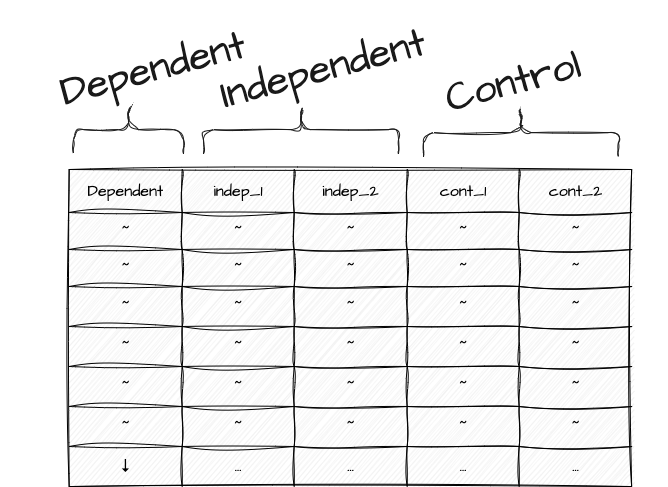
\includegraphics[width=0.5\textwidth,height=\textheight]{figures/approaching-analysis/aa-ida-variables.drawio.png}

}

\caption{\label{fig-aa-ida-variables}Roles of variables in IDA.}

\end{figure}

At this point let's look at the main characteristics that need to be
taken into account to statistically interrogate the variables we have
chosen to test our hypothesis. The type of statistical test that one
chooses is based on (1) the informational value of the dependent
variable and (2) the number of predictor variables included in the
analysis. Together these two characteristics go a long way in
determining the appropriate class of statistical test, but other
considerations about the distribution of particular variables
(i.e.~normality), relationships between variables (i.e.~independence),
and expected directionality of the predicted effect may condition the
appropriate method to be applied.

As you can imagine, there are a host of combinations and statistical
tests that apply in particular scenarios, too many to consider in given
the scope of this coursebook (see S. Th. Gries
(\protect\hyperlink{ref-Gries2013a}{2013}) and Paquot and Gries
(\protect\hyperlink{ref-Paquot2020a}{2020}) for a more exhaustive
description). Below I've summarized some common statistical scenarios
and their associated tests which focus on the juxtaposition of
informational values and the number of variables, leaving aside
alternative tests which deal with non-normal distributions, ordinal
variables, \emph{etc.}

In Table~\ref{tbl-ida-methods-monofactorial} we see
\textbf{monofactorial tests}, tests with only one predictor variable.

\hypertarget{tbl-ida-methods-monofactorial}{}
\begin{longtable}[]{@{}lll@{}}
\caption{\label{tbl-ida-methods-monofactorial}Common monofactorial tests
used in IDA.}\tabularnewline
\toprule\noalign{}
Dependent & Predictor & Test \\
\midrule\noalign{}
\endfirsthead
\toprule\noalign{}
Dependent & Predictor & Test \\
\midrule\noalign{}
\endhead
\bottomrule\noalign{}
\endlastfoot
Categorical & Categorical & Pearson's Chi-squared test \\
Numeric & Categorical & Student's t-Test \\
Numeric & Numeric & Pearson's correlation test \\
\end{longtable}

Table~\ref{tbl-ida-methods-multifactorial} includes a listing of
\textbf{multifactorial tests}, tests with more than one predictor and/
or control variables.

\hypertarget{tbl-ida-methods-multifactorial}{}
\begin{longtable}[]{@{}llll@{}}
\caption{\label{tbl-ida-methods-multifactorial}Common multifactorial
tests used in IDA.}\tabularnewline
\toprule\noalign{}
Dependent & Predictor & Control & Test \\
\midrule\noalign{}
\endfirsthead
\toprule\noalign{}
Dependent & Predictor & Control & Test \\
\midrule\noalign{}
\endhead
\bottomrule\noalign{}
\endlastfoot
Categorical & varied & varied & Logistic regression \\
Numeric & varied & varied & Linear regression \\
\end{longtable}

IDA relies heavily on quantitative evaluation methods to draw
conclusions that can be generalized to the target population. It is key
to understand that our goal in hypothesis testing is not to find
evidence in support of \(H_1\), but rather to assess the likelihood that
we can reliably reject \(H_0\). The metric used to determine if there is
sufficient evidence is based on the probability that given the nature of
the relationship and the characteristics of the data, the likelihood of
there being no difference or relationship is low. The threshold for
likelihood has traditionally been summarized in the \(p\)-value
statistic. In the Social Sciences, a \(p\)-value lower than .05 is
considered \emph{statistically significant} which when interpreted
correctly means that there is more than a 95\% chance that the observed
relationship would not be predicted by \(H_0\). Note that we are working
in the realm of probability, not in absolutes, therefore an analysis
that produces a significant result does not prove \(H_1\) is correct or
that \(H_0\) is incorrect, for that matter. A margin of error is always
present. For this reason, other metrics such as effect size and
confidence intervals are also used to interpret the results of
statistical tests.

\hypertarget{sec-aa-communicate}{%
\section{Communicate}\label{sec-aa-communicate}}

Conducting research should be enjoyable and personally rewarding but the
effort you have invested and knowledge you have generated should be
shared with others. Whether part of a blog, presentation, journal
article, or for your own purposes it is important to document your
analysis results and process in a way that is informative and
interpretable. This enhances the value of your work, allowing others to
learn from your experience and build on your findings.

\hypertarget{sec-aa-report}{%
\subsection{Report}\label{sec-aa-report}}

The most widely recognized form of communicating research is through a
report. A report is a narrative of your analysis, including the research
question, the data you used, the methods you applied, and the results
you obtained. We are both reporting our findings and documenting our
process to inform others of what we did and why we did it but also to
invite readers to evaluate our findings for themselves. The scientific
process is a collaborative one and evaluation by peers is a key
component of the process.

The audience for your report will determine the level of detail and the
type of information you will need to include in your report but there
are some common elements to reference in any report. First, the research
question and/ or hypothesis should be clearly stated and the motivation
for the question should be explained. This will help the reader
understand the context of the analysis and the importance of the
results. Second, diagnostic procedures to verifiy or describe the data
should be explained. This may include anomaly correction, missing data,
data transformation, etc. and/ or descriptive summaries of the data
including assessments of individual variables (central tendency,
dispersion, distribution) and/ or relationships between variables
(association strength). Third, a blueprint of the methods used will
describe the variable selection process, how the variables are
operationalized, what analysis methods are employed, and how the
variables are used in the statistical analysis. Fourth, the results from
the analysis are reported. Reporting details will depend on the type of
analysis and the particular method(s) employed. For inferential analyses
this will include the test statistic(s) and some measure of confidence.
In predictive analyses, accuracy results will be reported. For
exploratory analyses, the reporting of results will vary and often
include visualizations and metrics that require more human
interpretation than the other analysis types. Finally, the results are
interpreted in light of the research question and/ or hypothesis. This
will include a discussion of the limitations of the analysis and a
discussion of the implications of the results for future research.

\hypertarget{sec-aa-document}{%
\subsection{Document}\label{sec-aa-document}}

While a good report will include the most vital information to
understand the procedures, results, and findings of an analysis, there
is much more information generated in the course of an analysis which
does not traditionally appear in prose. If a research project is
conducted programmatically, however, data, code, and documentation can
be made available to others as part of the communication process.
Increasingly, researchers are sharing their data and code as part of the
publication process. This allows others to reproduce the analysis and
verify the results contributing to the collaborative nature of the
scientific process. \faIcon{wrench} {[}CITATION{]}

Together, data, code, and documentation form a \textbf{research
compendium}. As you can imagine the research process can quickly become
complex and unwieldy as the number of files and folders grows. If not
organized properly, it can be difficult to find the information you
need. Furthermore, if not documented, decisions made in the course of
the analysis can be difficult or impossible to trace. For this reason it
is recommendable to follow a set of best practices for organizing and
documenting your research compendium.

We will have more to say about this in the next chapter but for now it
will suffice to point to some key elements in a research compendium.
First, the data used in the analysis should be saved as a separate
file(s). As a given research project progresses to analysis, the data
may be transformed and manipulated to best fit the needs of the
analysis. Preserving the data at each stage adds to the complete picture
of the data from collection to analysis. Second, since you are working
programmatically, you can share your precise analysis step-by-step in
code form. This allows others to reproduce your analysis and verify your
results. Including code comments provides additional information to
communicate the steps taken and your thought process. Finally, a
codebook documents any additional information that helps understand the
research better. This will often include guides for installing software
and running the code to reproduce the analysis and an overview of the
aims of the scripts and the contents of the data and datasets.

\hypertarget{summary-2}{%
\section*{Summary}\label{summary-2}}
\addcontentsline{toc}{section}{Summary}

\markright{Summary}

In this chapter we have focused on description and analysis --the third
component of DIKI Hierarchy. This process is visually summarized in
Figure~\ref{fig-approaching-analysis-vis-sum}.

\begin{figure}[H]

{\centering 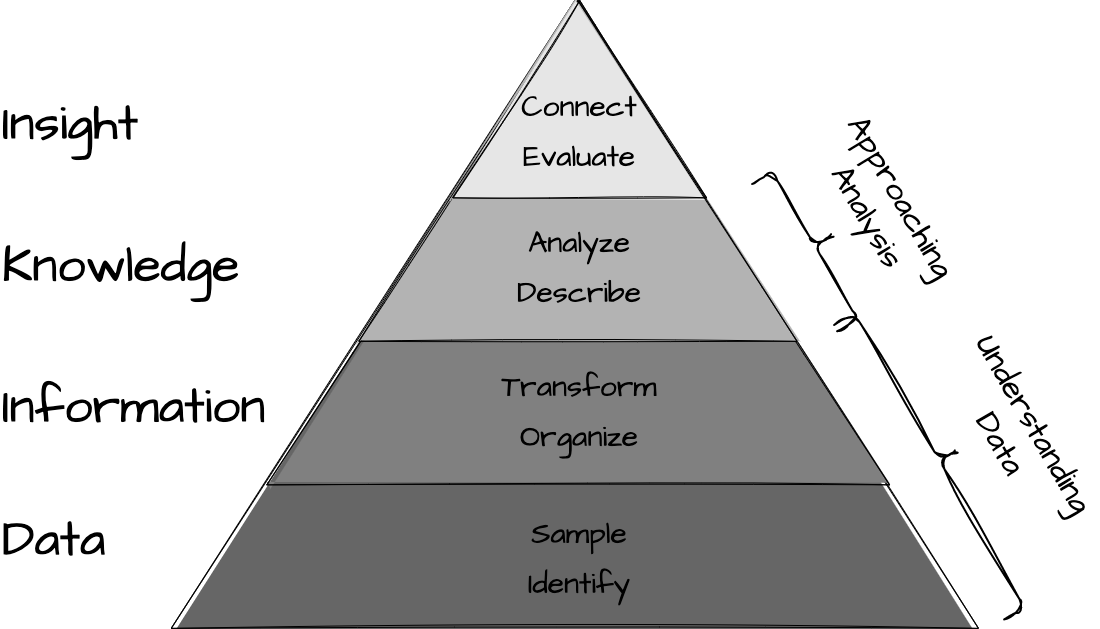
\includegraphics[width=0.75\textwidth,height=\textheight]{figures/approaching-analysis/aa-diki.drawio.png}

}

\caption{\label{fig-approaching-analysis-vis-sum}Approaching analysis:
visual summary}

\end{figure}

Building on the strategies covered in
\protect\hyperlink{sec-understanding-data}{Chapter 2 ``Understanding
data''} to derive a rich relational dataset, in this chapter we outlined
key points in approaching analysis. The first key step in any analysis
is to perform a diagnostic assessment of the individual variables and
relationships between variables. To select the appropriate descriptive
measures we covered the various informational values that a variable can
take. In addition to providing key information for reporting purposes,
descriptive measures are important to explore so the researcher can get
a better feel for the dataset before conducting an analysis.

We outlined three data analysis types in this chapter: exploratory,
predictive, and inferential. Each of these embodies distinct approaches
to deriving knowledge from data. Ultimately the choice of analysis type
is highly dependent on the goals of the research. Inferential analysis
is centered around the goal of testing a hypothesis, and for this reason
it is the most highly structured approach to analysis. This structure is
aimed at providing the mechanisms to draw conclusions from the results
that can be generalized to the target population. Predictive analysis
has a less-ambitious but at times more relevant goal of examining the
extent to which a given relationship can be established from the data to
provide a model of language that can accurately predict an outcome using
new data. This methodology is highly effective for applying different
algorithmic approaches and examining relationships between an outcome
variable and various configurations of variables. The ability to explore
the data in multiple ways, is also a key strength of employing an
exploratory analysis. The least structured and most variable of the
analysis types, exploratory analyses are a powerful approach to
generating knowledge from data in an area where clear predictions cannot
be made.

I rounded out this chapter with a short description of the importance of
communicating the analysis process and results. Reporting, in its
traditional form, is documented in prose in an article. This reporting
aims to provide the key information that a reader will need to
understand what was done, how it was done, and why it was done. This
information also provides the necessary information for reader's with a
critical eye to understand the analysis in more detail. Yet even the
most detailed reporting in a write-up still leaves many practical, but
key, points of the analysis obscured. A programming approach provides
the procedural steps taken that when shared provide the exact methods
applied. Together with the write-up, a research compendium which
provides the scripts to run the analysis and documentation on how to run
the analysis forms an integral part of creating reproducible research.

\hypertarget{activities-1}{%
\section*{Activities}\label{activities-1}}
\addcontentsline{toc}{section}{Activities}

\markright{Activities}

\begin{itemize}
\tightlist
\item[$\square$]
  \faIcon{wrench} Add description of outcomes \ldots{}
\end{itemize}

\begin{tcolorbox}[enhanced jigsaw, rightrule=.15mm, leftrule=.75mm, opacityback=0, arc=.35mm, colback=white, breakable, toprule=.15mm, bottomrule=.15mm, left=2mm]

\textbf{\faIcon{file-code} Recipe}

\textbf{What}:
\href{https://qtalr.github.io/qtalrkit/articles/recipe-3.html}{Descriptive
assessment of datasets}\\
\textbf{How}: Read Recipe 3 and participate in the Hypothes.is online
social annotation.\\
\textbf{Why}: To explore appropriate methods for summarizing variables
in datasets given the number and informational values of the
variable(s).

\end{tcolorbox}

\begin{tcolorbox}[enhanced jigsaw, rightrule=.15mm, leftrule=.75mm, opacityback=0, arc=.35mm, colback=white, breakable, toprule=.15mm, bottomrule=.15mm, left=2mm]

\textbf{\faIcon{flask} Lab}

\textbf{What}: \href{https://github.com/qtalr/lab-3}{Descriptive
assessment of datasets}\\
\textbf{How}: Clone, fork, and complete the steps in Lab 3.\\
\textbf{Why}: To identify and apply the appropriate descriptive methods
for a vector's informational value and to assess both single variables
and multiple variables with the appropriate statistical, tabular, and/
or graphical summaries.

\end{tcolorbox}

\hypertarget{questions-2}{%
\section*{Questions}\label{questions-2}}
\addcontentsline{toc}{section}{Questions}

\markright{Questions}

\begin{tcolorbox}[enhanced jigsaw, rightrule=.15mm, leftrule=.75mm, opacityback=0, arc=.35mm, colback=white, breakable, toprule=.15mm, bottomrule=.15mm, left=2mm]

\textbf{Conceptual questions}

\begin{itemize}
\tightlist
\item
  What are the key differences between assessment and analysis?
\item
  What are the potential measures of central tendency and dispersion for
  a variable? Does it depend on the informational value of the variable?
\item
  Consider the following variables: \(X\) = number of children, \(Y\) =
  number of siblings, \(Z\) = number of siblings who are older than the
  participant. Which of these variables are categorical, ordinal,
  numeric? What are the measures of central tendency and dispersion for
  each variable?
\item
  What type(s) of tables or plots are appropriate for summarizing a
  variable? What type(s) of tables or plots are appropriate for
  summarizing the relationship between two variables?
\item
  In the following variables and informational values, identify if the
  plots are appropriate for summarizing the relationship.\\
  \faIcon{wrench} \ldots{}
\item
  What are the key differences between exploratory, predictive, and
  inferential analysis?
\item
  How do the goals of the research influence the choice of analysis
  type?
\item
  Given the following research questions, identify which type of
  analysis is most appropriate and why.\\
  \faIcon{wrench} \ldots{}
\item
  How are the results of inferential, predictive, and exploratory
  analysis evaluated?
\item
  Research compendia are an important part of reproducible research.
  What are the key components of a research compendium? What are the
  benefits of sharing a research compendium?
\end{itemize}

\end{tcolorbox}

\begin{tcolorbox}[enhanced jigsaw, rightrule=.15mm, leftrule=.75mm, opacityback=0, arc=.35mm, colback=white, breakable, toprule=.15mm, bottomrule=.15mm, left=2mm]

\textbf{\faIcon{wrench} Technical exercises}

\begin{itemize}
\tightlist
\item
  Create a contingency table for the following variables:
\item
  Create a plot for the following variables:
\item
  Report these tables and plots with a short interpretation of what they
  show.
\item
  \ldots{}
\end{itemize}

\end{tcolorbox}

\hypertarget{sec-framing-research}{%
\chapter{Framing research}\label{sec-framing-research}}

\begin{tcolorbox}[enhanced jigsaw, leftrule=.75mm, title=\textcolor{quarto-callout-tip-color}{\faLightbulb}\hspace{0.5em}{Draft}, coltitle=black, opacityback=0, titlerule=0mm, arc=.35mm, bottomtitle=1mm, opacitybacktitle=0.6, colframe=quarto-callout-tip-color-frame, rightrule=.15mm, toptitle=1mm, left=2mm, colback=white, breakable, toprule=.15mm, bottomrule=.15mm, colbacktitle=quarto-callout-tip-color!10!white]

Ready for review.

\end{tcolorbox}

\begin{quote}
Thus, the task is, not so much to see what no one has seen yet; but to
think what nobody has thought yet, about that what everybody sees.

--- Arthur Schopenhauer
\end{quote}

\begin{tcolorbox}[enhanced jigsaw, rightrule=.15mm, leftrule=.75mm, opacityback=0, arc=.35mm, colback=white, breakable, toprule=.15mm, bottomrule=.15mm, left=2mm]

\textbf{\faIcon{list-alt} Outcomes}

\begin{itemize}
\tightlist
\item
  Identify a research area and problem by listing key strategies and
  describing their contribution towards research identification.
\item
  Explain the significance of a well-framed research question in guiding
  the overall research project.
\item
  Comprehend how the conceptual and practical steps involved in
  developing a research blueprint aid not only the researcher but also
  the broader scientific community.
\end{itemize}

\end{tcolorbox}

At this point in this part of the textbook, we have covered Data,
Information, and Knowledge from the Data to Insight Hierarchy. The goal
has been to provide an orientation to the main building blocks of doing
text analysis. Insight is the last component of the hierarchy. However,
in practical terms, it is the first step to address in an research
project as goals of a research project influence all subsequent steps.

In this chapter we discuss how to frame research, that is how to
position your research project's findings to contribute insight to
understanding of the world. We will cover how to connect with the
literature, selecting a research area and identifying a research
problem, and how to design research best positioned to return relevant
findings that will connect with this literature, establishing a research
aim and research question. We will round out this chapter with a guide
on developing a research blueprint --a working plan to organize the
conceptual and practical steps to implement the research effectively and
in a way that supports communicating the research findings and the
process by which the findings were obtained.

\begin{tcolorbox}[enhanced jigsaw, rightrule=.15mm, leftrule=.75mm, opacityback=0, arc=.35mm, colback=white, breakable, toprule=.15mm, bottomrule=.15mm, left=2mm]

\textbf{\faIcon{terminal} Swirl lesson}

\textbf{What}: \href{https://github.com/qtalr/lessons}{Version
control}\\
\textbf{How}: In the R Console pane load \texttt{swirl}, run
\texttt{swirl()}, and follow prompts to select the lesson.\\
\textbf{Why}: \faIcon{wrench} To \ldots.

\end{tcolorbox}

\hypertarget{sec-fr-frame}{%
\section{Frame}\label{sec-fr-frame}}

Together a research area, problem, aim and question and the research
blueprint that forms the conceptual and practical scaffolding of the
project ensure from the outset that the project is solidly grounded in
the main characteristics of good research. These characteristics,
summarized by Cross (\protect\hyperlink{ref-Cross2006}{2006}), are found
in Table~\ref{tbl-fr-cross-research-char-table}.

\hypertarget{tbl-fr-cross-research-char-table}{}
\begin{longtable}[]{@{}
  >{\raggedright\arraybackslash}p{(\columnwidth - 2\tabcolsep) * \real{0.1500}}
  >{\raggedright\arraybackslash}p{(\columnwidth - 2\tabcolsep) * \real{0.8500}}@{}}
\caption{\label{tbl-fr-cross-research-char-table}Characteristics of
research (Cross, 2006).}\tabularnewline
\toprule\noalign{}
\begin{minipage}[b]{\linewidth}\raggedright
Characteristic
\end{minipage} & \begin{minipage}[b]{\linewidth}\raggedright
Description
\end{minipage} \\
\midrule\noalign{}
\endfirsthead
\toprule\noalign{}
\begin{minipage}[b]{\linewidth}\raggedright
Characteristic
\end{minipage} & \begin{minipage}[b]{\linewidth}\raggedright
Description
\end{minipage} \\
\midrule\noalign{}
\endhead
\bottomrule\noalign{}
\endlastfoot
Purposive & Based on identification of an issue or problem worthy and
capable of investigation \\
Inquisitive & Seeking to acquire new knowledge \\
Informed & Conducted from an awareness of previous, related research \\
Methodical & Planned and carried out in a disciplined manner \\
Communicable & Generating and reporting results which are feasible and
accessible by others \\
\end{longtable}

With these characteristics in mind, let's get started with the first
component to address --connecting with the literature.

\hypertarget{sec-fr-connect}{%
\section{Connect}\label{sec-fr-connect}}

\hypertarget{research-area}{%
\subsection{Research area}\label{research-area}}

The first decision to make in the research process is to identify a
research area. A \textbf{research area} is a general area of interest
where a researcher wants to derive insight and make a contribution to
understanding. For those with an established research trajectory in
language, the area of research to address through text analysis will
likely be an extension of their prior work. For others, which include
new researchers or researcher's that want to explore new areas of
language research or approach an area through a language-based lens, the
choice of area may be less obvious. In either case, the choice of a
research area should be guided by a desire to contribute something
relevant to a theoretical, social, and/ or practical matter of personal
interest. Personal relevance goes a long way to developing and carrying
out \textbf{purposive} and \textbf{inquisitive} research.

So how do we get started? The first step is to reflect on your own areas
of interest and knowledge, be it academic, professional, or personal.
Language is at the heart of the human experience and therefore found in
some fashion anywhere one seeks to find it. But it is a big world and
more often than not the general question about what area to explore
language use is sometimes the most difficult. To get the ball rolling,
it is helpful to peruse disciplinary encyclopedias or handbooks of
linguistics and language-related an academic fields
(e.g.~\href{https://www.sciencedirect.com/referencework/9780080448541/encyclopedia-of-language-and-linguistics}{Encyclopedia
of Language and Linguistics} (\protect\hyperlink{ref-Brown2005}{Brown
2005}),
\href{https://www.sciencedirect.com/book/9781843345978/a-practical-guide-to-electronic-resources-in-the-humanities}{A
Practical Guide to Electronic Resources in the Humanities}
(\protect\hyperlink{ref-Dubnjakovic2010}{Dubnjakovic and Tomlin 2010}),
\href{https://www.routledgehandbooks.com/doi/10.4324/9781315749129}{Routledge
encyclopedia of translation technology}
(\protect\hyperlink{ref-Chan2014}{Chan 2014}))

A more personal, less academic, approach is to consult online forums,
blogs, \emph{etc}. that one already frequents or can be accessed via an
online search. For example, \href{https://www.reddit.com/}{Reddit} has a
wide variety of active subreddits
(\href{https://www.reddit.com/r/LanguageTechnology/}{r/LanguageTechnology},
\href{https://www.reddit.com/r/linguistics/}{r/Linguistics},
\href{https://www.reddit.com/r/corpuslinguistics/}{r/corpuslinguistics},
\href{https://www.reddit.com/r/DigitalHumanities/}{r/DigitalHumanities},
\emph{etc}.). Twitter and Facebook also have interesting posts on
linguistics and language-related fields worth following. Through one of
these social media site you may find particular people that maintain a
blog worth browsing. For example, I follow
\href{https://juliasilge.com/}{Julia Silge},
\href{http://www.rctatman.com/}{Rachel Tatman}, and
\href{https://tedunderwood.com/}{Ted Underwood}, \emph{inter alia}.
Perusing these resources can help spark ideas and highlight the kinds of
questions that interest you.

Regardless of whether your inquiry stems from academic, professional, or
personal interest, try to connect these findings to academic areas of
research. Academic research is highly structured and well-documented and
making associations with this network will aid in subsequent steps in
developing a research project.

\hypertarget{sec-fr-problem}{%
\subsection{Research problem}\label{sec-fr-problem}}

Once you've made a rough-cut decision about the area of research, it is
now time to take a deeper dive into the subject area and jump into the
literature. This is where the rich structure of disciplinary research
will provide aid to traverse the vast world of academic knowledge and
identify a research problem. A \textbf{research problem} highlights a
particular topic of debate or uncertainty in existing knowledge which is
worthy of study.

Surveying the relevant literature is key to ensuring that your research
is \textbf{informed}, that is, connected to previous work. Identifying
relevant research to consult can be a bit of a `chicken or the egg'
problem --some knowledge of the area is necessary to find relevant
topics, some knowledge of the topics is necessary to narrow the area of
research. Many times the only way forward is to jump into conducting
searches. These can be world-accessible resources (\emph{e.g.}
\href{https://scholar.google.com/}{Google Scholar}) or limited-access
resources that are provided through an academic institution (\emph{e.g.}
\href{https://about.proquest.com/en/products-services/llba-set-c}{Linguistics
and Language Behavior Abstracts}), \href{https://eric.ed.gov/}{ERIC},
\href{https://www.ebsco.com/products/research-databases/apa-psycinfo}{PsycINFO},
\emph{etc.}). Some organizations and academic institutions provide
\href{https://guides.zsr.wfu.edu/linguistics}{research guides} to help
researcher's access the primary literature.

Another avenue to explore are journals dedicated to areas in which
linguistics and language-related research is published. In
Table~\ref{tbl-pinboard-journals-linguistics},
Table~\ref{tbl-pinboard-journals-humanities}, and
Table~\ref{tbl-pinboard-journals-cl}, I've listed a number of highly
visible journals in linguistics, digital humanities, and computational
linguistics.

\hypertarget{tbl-pinboard-journals-linguistics}{}
\begin{longtable}[]{@{}
  >{\raggedright\arraybackslash}p{(\columnwidth - 2\tabcolsep) * \real{0.3000}}
  >{\raggedright\arraybackslash}p{(\columnwidth - 2\tabcolsep) * \real{0.7000}}@{}}
\caption{\label{tbl-pinboard-journals-linguistics}A list of some
linguistics journals.}\tabularnewline
\toprule\noalign{}
\begin{minipage}[b]{\linewidth}\raggedright
Resource
\end{minipage} & \begin{minipage}[b]{\linewidth}\raggedright
Description
\end{minipage} \\
\midrule\noalign{}
\endfirsthead
\toprule\noalign{}
\begin{minipage}[b]{\linewidth}\raggedright
Resource
\end{minipage} & \begin{minipage}[b]{\linewidth}\raggedright
Description
\end{minipage} \\
\midrule\noalign{}
\endhead
\bottomrule\noalign{}
\endlastfoot
Corpora & An international, peer-reviewed journal of corpus linguistics
focusing on the many and varied uses of corpora both in linguistics and
beyond. \\
Corpus Linguistics and Linguistic Theory & Corpus Linguistics and
Linguistic Theory (CLLT) is a peer-reviewed journal publishing
high-quality original corpus-based research focusing on theoretically
relevant issues in all core areas of linguistic research, or other
recognized topic areas. \\
International Journal of Corpus Linguistics & The International Journal
of Corpus Linguistics (IJCL) publishes original research covering
methodological, applied and theoretical work in any area of corpus
linguistics. \\
International Journal of Language Studies & It is a refereed
international journal publishing articles and reports dealing with
theoretical as well as practical issues focusing on language,
communication, society and culture. \\
Journal of Child Language & A key publication in the field, Journal of
Child Language publishes articles on all aspects of the scientific study
of language behaviour in children, the principles which underlie it, and
the theories which may account for it. \\
Journal of Linguistic Geography & The Journal of Linguistic Geography
focuses on dialect geography and the spatial distribution of language
relative to questions of variation and change. \\
Journal of Quantitative Linguistics & Publishes research on the
quantitative characteristics of language and text in mathematical form,
introducing methods of advanced scientific disciplines. \\
\end{longtable}

\hypertarget{tbl-pinboard-journals-humanities}{}
\begin{longtable}[]{@{}
  >{\raggedright\arraybackslash}p{(\columnwidth - 2\tabcolsep) * \real{0.3000}}
  >{\raggedright\arraybackslash}p{(\columnwidth - 2\tabcolsep) * \real{0.7000}}@{}}
\caption{\label{tbl-pinboard-journals-humanities}A list of some
humanities journals.}\tabularnewline
\toprule\noalign{}
\begin{minipage}[b]{\linewidth}\raggedright
Resource
\end{minipage} & \begin{minipage}[b]{\linewidth}\raggedright
Description
\end{minipage} \\
\midrule\noalign{}
\endfirsthead
\toprule\noalign{}
\begin{minipage}[b]{\linewidth}\raggedright
Resource
\end{minipage} & \begin{minipage}[b]{\linewidth}\raggedright
Description
\end{minipage} \\
\midrule\noalign{}
\endhead
\bottomrule\noalign{}
\endlastfoot
Digital Humanities Quarterly & Digital Humanities Quarterly (DHQ), an
open-access, peer-reviewed, digital journal covering all aspects of
digital media in the humanities. \\
Digital Scholarship in the Humanities & DSH or Digital Scholarship in
the Humanities is an international, peer reviewed journal which
publishes original contributions on all aspects of digital scholarship
in the Humanities including, but not limited to, the field of what is
currently called the Digital Humanities. \\
Journal of Cultural Analytics & Cultural Analytics is an open-access
journal dedicated to the computational study of culture. Its aim is to
promote high quality scholarship that applies computational and
quantitative methods to the study of cultural objects (sound, image,
text), cultural processes (reading, listening, searching, sorting,
hierarchizing) and cultural agents (artists, editors, producers,
composers). \\
\end{longtable}

\hypertarget{tbl-pinboard-journals-cl}{}
\begin{longtable}[]{@{}
  >{\raggedright\arraybackslash}p{(\columnwidth - 2\tabcolsep) * \real{0.3000}}
  >{\raggedright\arraybackslash}p{(\columnwidth - 2\tabcolsep) * \real{0.7000}}@{}}
\caption{\label{tbl-pinboard-journals-cl}A list of some computational
linguistics journals.}\tabularnewline
\toprule\noalign{}
\begin{minipage}[b]{\linewidth}\raggedright
Resource
\end{minipage} & \begin{minipage}[b]{\linewidth}\raggedright
Description
\end{minipage} \\
\midrule\noalign{}
\endfirsthead
\toprule\noalign{}
\begin{minipage}[b]{\linewidth}\raggedright
Resource
\end{minipage} & \begin{minipage}[b]{\linewidth}\raggedright
Description
\end{minipage} \\
\midrule\noalign{}
\endhead
\bottomrule\noalign{}
\endlastfoot
Computational Linguistics & Computational Linguistics is the
longest-running publication devoted exclusively to the computational and
mathematical properties of language and the design and analysis of
natural language processing systems. \\
LREC Conferences & The International Conference on Language Resources
and Evaluation is organised by ELRA biennially with the support of
institutions and organisations involved in HLT. \\
Transactions of the Association for Computational Linguistics &
Transactions of the Association for Computational Linguistics (TACL) is
an~ACL-sponsored journal~published by MIT Press~that publishes papers in
all areas of computational linguistics and natural language
processing. \\
\end{longtable}

To explore research related to text analysis it is helpful to start with
the (sub)discipline name(s) you identified in when selecting your
research area, more specific terms that occur to you or key terms from
the literature, and terms such as `corpus study' or `corpus-based'. The
results from first searches may not turn out to be sources that end up
figuring explicitly in your research, but it is important to skim these
results and the publications themselves to mine information that can be
useful to formulate better and more targeted searches. Relevant
information for honing your searches can be found throughout an academic
publication (article or book). However, pay particular attention to the
abstract, in articles, and the table of contents, in books, and the
cited references. Abstracts and tables of contents often include
discipline-specific jargon that is commonly used in the field. In some
articles there is even a short list of key terms listed below the
abstract which can be extremely useful to seed better and more precise
search results. The references section will contain relevant and
influential research. Scan these references for publications which
appear to narrowing in on topic of interest and treat it like a search
in its own right.

Once your searches begin to show promising results it is time to keep
track and organize these references. Whether you plan to collect
thousands of references over a lifetime of academic research or your aim
is centered around one project, software such as
\href{https://www.zotero.org/}{Zotero}\footnote{\href{https://guides.zsr.wfu.edu/zotero}{Zotero
  Guide}},
\href{https://www.mendeley.com/reference-management/reference-manager}{Mendeley},
or \href{https://bibdesk.sourceforge.io/}{BibDesk} provide powerful,
flexible, and easy-to-use tools to collect, organize, annotate, search,
and export references. Citation management software is indispensable for
modern research --and often free!

As your list of relevant references grows, you will want to start the
investigation process in earnest. Begin skimming (not reading) the
contents of each of these publications, starting with the most relevant
first\footnote{Or what appears to be most relevant. This may change as
  you start to take a closer look.}. Annotate these publications using
highlighting features of the citation management software to identify:
(1) the stated goal(s) of the research, (2) the data source(s) used, (3)
the information drawn from the data source(s), (4) the analysis approach
employed, and (5) the main finding(s) of the research as they pertain to
the stated goal(s). Next, in your own words, summarize these five key
areas in prose adding your summary to the notes feature of the citation
management software. This process will allow you to efficiently gather
and document references with the relevant information to guide the
identification of a research problem, to guide the formation of your
problem statement, and ultimately, to support the literature review that
will figure in your project write-up.

From your preliminary annotated summaries you will undoubtedly start to
recognize overlapping and contrasting aspects in the research
literature. These aspects may be topical, theoretical, methodological,
or appear along other lines. Note these aspects and continue to conduct
more refine searches, annotate new references, and monitor for any
emerging patterns of uncertainty or debate (gaps) which align with your
research interest(s). When a promising pattern takes shape, it is time
to engage with a more detailed reading of those references which appear
most relevant highlighting the potential gap(s) in the literature.

At this point you can focus energy on more nuanced aspects of a
particular gap in the literature with the goal to formulate a problem
statement. A \textbf{problem statement} directly acknowledges a gap in
the literature and puts a finer point on the nature and relevance of
this gap for understanding. This statement reflects your first
deliberate attempt to establish a line of inquiry. It will be a
targeted, but still somewhat general, statement framing the gap in the
literature that will guide subsequent research design decisions.

\hypertarget{sec-fr-define}{%
\section{Define}\label{sec-fr-define}}

\hypertarget{sec-fr-aim}{%
\subsection{Research aim}\label{sec-fr-aim}}

With a problem statement in hand, it is now time to consider the goal(s)
of the research. A \textbf{research aim} frames the type of inquiry to
be conducted. Will the research aim to explore, examine, or explain? In
other words, will the research seek to uncover novel relationships,
assess the potential strength of a particular relationship, or test a
particular relationship? As you can appreciate, the research aim is
directly related to the analysis methods we touched upon in
\protect\hyperlink{sec-approaching-analysis}{Chapter 3}.

To gauge how to frame your research aim, reflect on the literature that
led you to your problem statement and the nature of the problem
statement itself. If the gap at the center of the problem statement is a
lack of knowledge, your research aim may be exploratory. If the gap
concerns a conjecture about a relationship, then your research may take
a predictive approach. When the gap points to the validation of a
relationship, then your research will likely be inferential in nature.
Before selecting your research aim it is also helpful to consult the
research aims of the primary literature that led you to your research
statement.

Typically, a problem statement addressing a subtle, specific issue tends
to adopt research objectives similar to prior studies. In contrast, a
statement focusing on a broader, more distinct issue is likely to have
unique research goals. Yet, this is more of a guideline than a strict
rule.

It's crucial to understand both the existing literature and the nature
of various types of analyses. Being clear about your research goals is
important to ensure that your study is well-placed to produce results
that add value to the current understanding in an informed manner.

\hypertarget{sec-fr-question}{%
\subsection{Research question}\label{sec-fr-question}}

The next step in research design is to craft the research question. A
\index{research question}\textbf{research question} is clearly defined
statement which identifies an aspect of uncertainty and the particular
relationships that this uncertainty concerns. The research question
extends and narrows the line of inquiry established in the research
statement and research aim. To craft a research question, we can use the
research statment for the content and the research aim for the form.

\hypertarget{sec-fr-question-form}{%
\subsubsection{Form}\label{sec-fr-question-form}}

The form of a research question will vary based on the research aim,
which as I mentioned, is inimately connected to the analysis approach.
For inferential-based research, the research question will actually be a
statement, not a question. This statement makes a testable claim about
the nature of a particular relationship --\emph{i.e.} asserts a
hypothesis.

For illustration, let's return to the hypothesis (\(H_1\)) we previously
sketched out in \protect\hyperlink{sec-approaching-analysis}{Chapter 3},
leaving aside the implicit null hypothesis, seen in
Example~\ref{exm-fr-form-infer}.

\begin{example}[]\protect\hypertarget{exm-fr-form-infer}{}\label{exm-fr-form-infer}

Women use more questions than men in spontaneous conversations.

\end{example}

For predictive- and exploratory-based research, the research question is
in fact a question. A reframing of the example hypothesis for a
predictive-based research question might take the form seen in
Example~\ref{exm-fr-form-pred}.

\begin{example}[]\protect\hypertarget{exm-fr-form-pred}{}\label{exm-fr-form-pred}

Can the number of questions used in spontaneous conversations predict if
a speaker is male or female?

\end{example}

And a similar exploratory-based research question might take the form
seen in Example~\ref{exm-fr-form-exp}.

\begin{example}[]\protect\hypertarget{exm-fr-form-exp}{}\label{exm-fr-form-exp}

Do men and women differ in terms of the number of questions they use in
spontaneous conversations?

\end{example}

The central research interest behind these hypothetical research
questions is, admittedly, quite basic. But from these simplified
examples, we are able to appreciate the similarities and differences
between the forms of research statements that correspond to distinct
research aims.

\hypertarget{sec-fr-question-content}{%
\subsubsection{Content}\label{sec-fr-question-content}}

In terms of content, the research question will make reference to two
key components. First, is the unit of analysis. The \textbf{unit of
analysis} is the entity which the research aims to investigate. For our
three example research aims, the unit of analysis is the same, namely
\emph{speakers}. Note, however, that the current unit of analysis is
somewhat vague in the example research questions. A more precise unit of
analysis would include more information about the population from which
the speakers are drawn (\emph{i.e.} English speakers, American English
speakers, American English speakers of the Southeast, \emph{etc}.).

The second key component is the unit of observation. The \textbf{unit of
observation} is the primary element on which the insight into the unit
of analysis is derived and in this way constitutes the essential
organizational unit of the dataset to be analyzed. In our examples, the
unit of observation, again, is unchanged and is \emph{spontaneous
conversations}. Note that while the unit of observation is key to
identify as it forms the organizational backbone of the research, it is
very common for the research to derive variables from this unit to
provide evidence to investigate the research question.

In examples \ref{exm-fr-form-infer}, \ref{exm-fr-form-pred}, and
\ref{exm-fr-form-exp}, we identified the number of conversations as part
of the research question. Later in the research process it will be key
to operationalize this variable. For example, will the number of
conversations be the total number of conversations in the dataset or
will it be the average number of conversations per speaker? These are
important questions to consider as they will influence variable
selection, statistical choices, and ultimately the interpretation of the
results.

\hypertarget{sec-fr-blueprint}{%
\section{Blueprint}\label{sec-fr-blueprint}}

Efforts to craft a research question are a very important aspect of
developing purposive, inquisitive, and informed research (returning to
Cross's characteristics of research). Moving beyond the research
question in the project means developing and laying out the research
design in a way such that the research is \textbf{Methodical} and
\textbf{Communicable}. In this textbook, the method to achieve these
goals is through the development of a research blueprint. The blueprint
includes two components: (1) laying out a conceptual plan and (2)
deriving the organizational scaffolding that will support the
implementation of the research.

As Ignatow and Mihalcea (\protect\hyperlink{ref-Ignatow2017}{2017})
point out:

\begin{quote}
Research design is essentially concerned with the basic architecture of
research projects, with designing projects as systems that allow theory,
data, and research methods to interface in such a way as to maximize a
project's ability to achieve its goals {[}\ldots{]}. Research design
involves a sequence of decisions that have to be taken in a project's
early stages, when one oversight or poor decision can lead to results
that are ultimately trivial or untrustworthy. Thus, it is critically
important to think carefully and systematically about research design
before committing time and resources to acquiring texts or mastering
software packages or programming languages for your text mining project.
\end{quote}

In what follows, I will cover the main aspects of developing a research
blueprint. I will start with the conceptual plan and then move on to the
organizational scaffolding.

\hypertarget{sec-fr-plan}{%
\subsection{Plan}\label{sec-fr-plan}}

Importance of establishing a feasible research design from the outset
and documenting the key aspects required to conduct the research cannot
be understated. On the one hand this process links a conceptual plan to
a tangible implementation. In doing so, a researcher is
better-positioned to conduct research with a clear view of what will be
entailed. On the other hand, a promising research question may present
unexpected challenges once a researcher sets about to implement the
research. This is not uncommon to encounter issues that require
modification or reevaluation of the viability of the project. However, a
well-documented research plan will help a researcher to identify and
address many of these challenges at the conceptual level before
expending effort on the implementation.

Let's now consider the main aspects of developing a research plan:
identifying data source(s), key variables, and analysis methods. Before
we do, however, it is important to reiterate the importance of a
research question or hypothesis before moving forward in research
planning. The research question or hypothesis is the central component
of the research plan. It guides every step which follows from data
selection to interpretation of the analysis results. Furthermore, a
well-founded research question is based on a solid literature review
from which can provide helpful guidance at key choice points in the
research process.

First, \textbf{identify a viable data source}. Viability includes the
accessibility of the data, availability of the data, and the content of
the data. If a purported data source is not accessible and/ or is has
stringent restrictions on its use, then it is not a viable data source.
If a data source is accessible and available, but does not contain the
building blocks needed to address the research question, then it is not
a viable data source. In the case that research is inferential in
nature, the sampling frame of the corpus is of primary importance as the
goal is to generalize the findings to a target population. A corpus
resource should align, to the extent feasible, with this target
population. For predictive and exploratory research, the goal to
generalize a claim is not central and for this reason the there is some
freedom in terms of how representative a corpus sample is of a target
population. Ideally, a researcher will find and be able to model a
language population of target interest. Since the goal, however, is not
to test a hypothesis, but rather to explore particular or evaluate
potential relationships, either in an exploratory or predictive fashion,
the research can often continue with the stipulation that the results
are interpreted in the light of the characteristics of the available
corpus sample.

The second step is to \textbf{identify the key variables} need to
conduct the research are and then ensure that this information can be
derived from the corpus data. The research question will reference the
unit of analysis and the unit of observation, but it is important at
this point to then pinpoint what the key variables will be. If the unit
of observation is spontaneous conversations. The question as to what
aspects of these conversations will be used in the analysis. In the
research questions presented in this chapter, we will want to envision
what needs to be done to derive a variable which measures the number of
questions in each of the conversations. In other research, their may be
features that need to be extracted, recoded, and/ or generated to
address the research question. Other variables of importance may be
non-linguistic in nature. In cases where there the metadata is
incomplete for the goals of the research, it is sometimes possible to
merge metadata from other sources.

The third step is to \textbf{identify a method of analysis} to
interrogate the dataset. The selection of the analysis approach that was
part of the research aim (\emph{i.e.} explore, predict, or infer) and
then the research question goes a long way to narrowing the methods that
a researcher must consider. But there are a number of factors which will
make some methods more appropriate than others.

Exploratory research is the least restricted of the three types of
analysis approaches. Although it may be the case that a research will
not be able to specify from the outset of a project what the exact
analysis methods will be, an attempt to consider what types of analysis
methods will be most promising to provide results to address the
research question goes a long way to steering a project in the right
direction and grounding the research. As with the other analysis
approaches, it is important to be aware of what the analysis methods
available and what type of information they produce in light of the
research question.

For predictive-based research, the informational value of the target
variable is key to deciding whether the prediction will be a
classification task or a regression task. This has downstream effects
when it comes time to evaluate and interpret the results. Although the
feature engineering process in predictive analyses means that the
features do not need to be specified from the outset and can be tweaked
and changed as needed during an analysis, it is a good idea to start
with a basic sense of what features most likely will be helpful in
developing a robust predictive model. Furthermore, while the number and
informational values of the features (predictor variables) are not as
important to selecting a prediction method (algorithm) as they are in
inferential analysis methods, it is important to recognize that
particular algorithms have strengths and shortcomings when working large
numbers and/ or types of features
(\protect\hyperlink{ref-Lantz2013}{Lantz 2013}).

In inferential research, the number and information values of the
variables to be analyzed will be of key importance
(\protect\hyperlink{ref-Gries2013a}{S. Th. Gries 2013}). The
informational value of the dependent variable will again narrow the
search for the appropriate method. The number of predictor variables
also plays an important role. For example, a study with a categorical
dependent variable with a single categorical predictor variable will
lead the researcher to the Chi-squared test. A study with a numeric
dependent variable with multiple predictor variables will lead to linear
regression. Another aspect of note for inference studies is the
consideration of the distribution of numeric variables --a normal
distribution will use a parametric test where a non-normal distribution
will use a non-parametric test. These details need not be nailed down at
this point, but it is helpful to have them on your radar to ensure that
when the time comes to analyze the data, the appropriate steps are taken
to test for normality and then apply the correct test.

The last of the main components of the research plan concerns the
\textbf{interpretation and evaluation of the results}. This step brings
the research plan full circle connecting the research question to the
methods employed. It is important to establish from the outset what the
criteria will be to evaluate the results. This is in large part a
function of the relationship between the research question and the
analysis method. For example, in exploratory research, the results will
be evaluated qualitatively in terms of the associative patterns that
emerge. Predictive and inferential research leans more heavily on
quantitative metrics in particular the accuracy of the prediction or the
strength of the relationship between the dependent and predictor
variable(s), respectively. However, these quantitative metrics require
qualitative interpretation to determine whether the results are
meaningful in light of the research question.

To summarize these planning steps, I've created a checklist in
Table~\ref{tbl-fr-plan-checklist}.

\hypertarget{tbl-fr-plan-checklist}{}
\begin{longtable}[]{@{}
  >{\raggedright\arraybackslash}p{(\columnwidth - 2\tabcolsep) * \real{0.2500}}
  >{\raggedright\arraybackslash}p{(\columnwidth - 2\tabcolsep) * \real{0.7500}}@{}}
\caption{\label{tbl-fr-plan-checklist}Research Plan
Checklist}\tabularnewline
\toprule\noalign{}
\begin{minipage}[b]{\linewidth}\raggedright
Steps
\end{minipage} & \begin{minipage}[b]{\linewidth}\raggedright
Description
\end{minipage} \\
\midrule\noalign{}
\endfirsthead
\toprule\noalign{}
\begin{minipage}[b]{\linewidth}\raggedright
Steps
\end{minipage} & \begin{minipage}[b]{\linewidth}\raggedright
Description
\end{minipage} \\
\midrule\noalign{}
\endhead
\bottomrule\noalign{}
\endlastfoot
Research Question or Hypothesis & Formulate a research question or
hypothesis based on a thorough review of existing literature including
references. This will guide every subsequent step from data selection to
interpretation of results. \\
Data Source(s) & Identify viable data source(s) and vet the sample data
in light of the research question. Consider to what extent the goal is
to generalize findings to a target population, and ensure that the
corpus aligns as much as feasible with this target. \\
Key Variables & Determine the key variables needed for the research,
define how they will be operationalized, and ensure they can be derived
from the corpus data. Additionally, identify any features that need to
be extracted, recoded or generated. \\
Analysis Method & Choose an appropriate method of analysis to
interrogate the dataset. This choice should be in line with your
research aim (\emph{e.g.}, exploratory, predictive, inferential). Be
aware of what each method can offer and how it addresses your research
question. \\
Interpretation \& Evaluation & Establish criteria to interpret and
evaluate the results. This will be a function of the relationship
between the research question and the analysis method. \\
\end{longtable}

In addition to addressing the steps outlined in
Table~\ref{tbl-fr-plan-checklist}, it is also important to document the
strengths and shortcomings of the research plan including the data
source(s), the information to be extracted from the data, and the
analysis methods. If there are potential shortcomings, which there most
often are, sketch out contingency plans to address these shortcomings.
This will help buttress your research and ensure that your time and
effort is well-spent.

Together the information collected from this process will serve to guide
the research and provide a solid foundation for the research write-up.
Furthermore, you may consider pre-registering your research project to
ensure that your plans are well-documented and to provide a timestamp
for your research. Pre-registration can also be a helpful way to get
feedback on your research plan from colleagues and experts in the field.
Popular pre-registration platforms include \href{https://osf.io/}{Open
Science Framework} and
\href{https://www.cos.io/initiatives/prereg}{Center for Open Science}.

\hypertarget{sec-fr-scaffold}{%
\subsection{Scaffold}\label{sec-fr-scaffold}}

The next step in creating a research blueprint is to consider how to
physically implement your project. This includes how to organize files
and directories in a fashion that both provides the researcher a logical
and predictable structure to work with but also ensures that the
research is \textbf{Communicable}. On the one hand, communicable
research includes a strong write-up of the research, but, on the other
hand, it is also important that the research is reproducible.
Reproducibility strategies are a benefit to the researcher (in the
moment and in the future) as it leads to better work habits and to
better teamwork and it makes changes to the project easier.
Reproducibility is also of benefit to the scientific community as shared
reproducible research enhances replicability and encourages cumulative
knowledge development (\protect\hyperlink{ref-Gandrud2015}{Gandrud
2015}).

There are a set of guiding principles to accomplish these goals
(\protect\hyperlink{ref-Gentleman2007}{Gentleman and Temple Lang 2007};
\protect\hyperlink{ref-Marwick2018}{Marwick, Boettiger, and Mullen
2018}), seen in Example~\ref{exm-fr-repro-principles}.

\begin{example}[]\protect\hypertarget{exm-fr-repro-principles}{}\label{exm-fr-repro-principles}

Reproducible Research Principles

\begin{enumerate}
\def\labelenumi{\arabic{enumi}.}
\tightlist
\item
  All files should be plain text which means they contain no formatting
  information other than whitespace.
\item
  There should be a clear separation between the data, method, and
  output of research. This should be apparent from the directory
  structure.
\item
  A separation between original, derived, and analysis data should be
  made. Original data should be treated as `read-only'. Any changes to
  the original data should be justified, generated by the code, and
  documented (see point 6).
\item
  Each project file (script) should represent a particular, well-defined
  step in the research process.
\item
  Each project script should be modular --that is, each file should
  correspond to a specific goal in the analysis procedure with input and
  output only corresponding to this step.
\item
  All project scripts should be tied together by a `main' script that is
  used to coordinate the execution of all the project steps.
\item
  Everything should be documented. This includes data collection, data
  preprocessing, analysis steps, script code comments, data description
  in data dictionaries, information about the computing environment and
  packages used to conduct the analysis, and detailed instructions on
  how to reproduce the research.
\end{enumerate}

\end{example}

These seven principles can be physically implemented in numerous ways.
In recent years, there has been a growing number of efforts to create R
packages and templates to quickly generate the scaffolding and tools to
facilitate reproducible research. Some notable R packages include
\href{https://jdblischak.github.io/workflowr/}{workflowr}
(\protect\hyperlink{ref-R-workflowr}{Blischak, Carbonetto, and Stephens
2021}), \href{http://projecttemplate.net/}{ProjectTemplate}
(\protect\hyperlink{ref-R-ProjectTemplate}{White 2023}), and
\href{https://github.com/ropensci/targets}{targets}
(\protect\hyperlink{ref-R-targets}{Landau 2023}), but there are many
other resources for R included on the
\href{https://cran.r-project.org/web/views/ReproducibleResearch.html}{CRAN
Task View for Reproducible Research}. There are many advantages to
working with pre-existing frameworks for the savvy R programmer
including the ability to quickly generate a project scaffold, to
efficiently manage changes to the project, and to buy in to a common
framework that is supported by a community of developers.

On the other hand, these frameworks can be a bit daunting for the novice
R programmer. At the most basic level, a project can implement the seven
principles outlined above by creating a directory structure and a set of
files manually.

\begin{example}[]\protect\hypertarget{exm-fr-basic-project}{}\label{exm-fr-basic-project}

Minimal Project Framework

\begin{Shaded}
\begin{Highlighting}[]
\ExtensionTok{project/}
\ExtensionTok{├──}\NormalTok{ data/}
\ExtensionTok{│}\NormalTok{   ├── analysis/}
\ExtensionTok{│}\NormalTok{   ├── derived/}
\ExtensionTok{│}\NormalTok{   └── original/}
\ExtensionTok{├──}\NormalTok{ output/}
\ExtensionTok{│}\NormalTok{   ├── figures/}
\ExtensionTok{│}\NormalTok{   ├── reports/}
\ExtensionTok{│}\NormalTok{   ├── results/}
\ExtensionTok{│}\NormalTok{   └── tables/}
\ExtensionTok{├──}\NormalTok{ code/}
\ExtensionTok{│}\NormalTok{   └── ...}
\ExtensionTok{├──}\NormalTok{ \_main.R}
\ExtensionTok{└──}\NormalTok{ README}
\end{Highlighting}
\end{Shaded}

\end{example}

In Example~\ref{exm-fr-basic-project}, I provide a minimal framework
that aligns with the reproducible research principles. Let me now make
the connections between the principles and this project structure.

The \emph{project/} directory is composed of three main sections:
\emph{data/}, \emph{output/}, and \emph{code/} corresponding to the
input, output, and code, respectively.

The \emph{data/} section is divided into three subsections:

\begin{itemize}
\tightlist
\item
  \emph{analysis/} for storing data used to perform analysis
\item
  \emph{derived/} for housing data produced in curation and
  transformation steps
\item
  \emph{original/} for keeping the original `read-only' data
\end{itemize}

The \emph{output/} section contains four subsections:

\begin{itemize}
\tightlist
\item
  \emph{figures/} for visualizations produced as part of the project
\item
  \emph{reports/} for the resulting reports (\emph{e.g.} article,
  presentation, blog post, \emph{etc.})
\item
  \emph{results/} for statistical results from the analysis
\item
  \emph{tables/} for summary tables
\end{itemize}

The \emph{code/} directory houses the code, with the \emph{\_main.R}
file at the root of the project orchestrating the execution of all
project steps.

Lastly, the \emph{README} file provides a description of the project and
instructions on how to reproduce the research.

The project structure in Example~\ref{exm-fr-basic-project} meets the
minimal structural requirements for reproducible research but can be
augmented in more sophisticated ways to support more functionality, as
we will see in Chapter~\ref{sec-collaboration}. One enhancement that I
highly recommend is the use of literate programming, in the form of
Quarto documents, to serve as the main project scripts. This facilitates
the combination of executable code and prose documentation for each
project step in a single, modular file.

\hypertarget{summary-3}{%
\section*{Summary}\label{summary-3}}
\addcontentsline{toc}{section}{Summary}

\markright{Summary}

The aim of this chapter is to provide the key conceptual and practical
points to guide the development of a viable research project. Good
research is purposive, inquisitive, informed, methodological, and
communicable. It is not, however, always a linear process. Exploring
your area(s) of interest and connecting with existing work will help
couch and refine your research. But practical considerations, such as
the existence of viable data, technical skills, and/ or time constrains,
sometimes pose challenges and require a researcher to rethink and/ or
redirect the research in sometimes small and other times more
significant ways. The process of formulating a research question and
developing a viable research plan is key to supporting viable,
successful, and insightful research. To ensure that the effort to derive
insight from data is of most value to the researcher and the research
community, the research should strive to be methodological and
communicable adopting best practices for reproducible research.

\begin{figure}[H]

{\centering 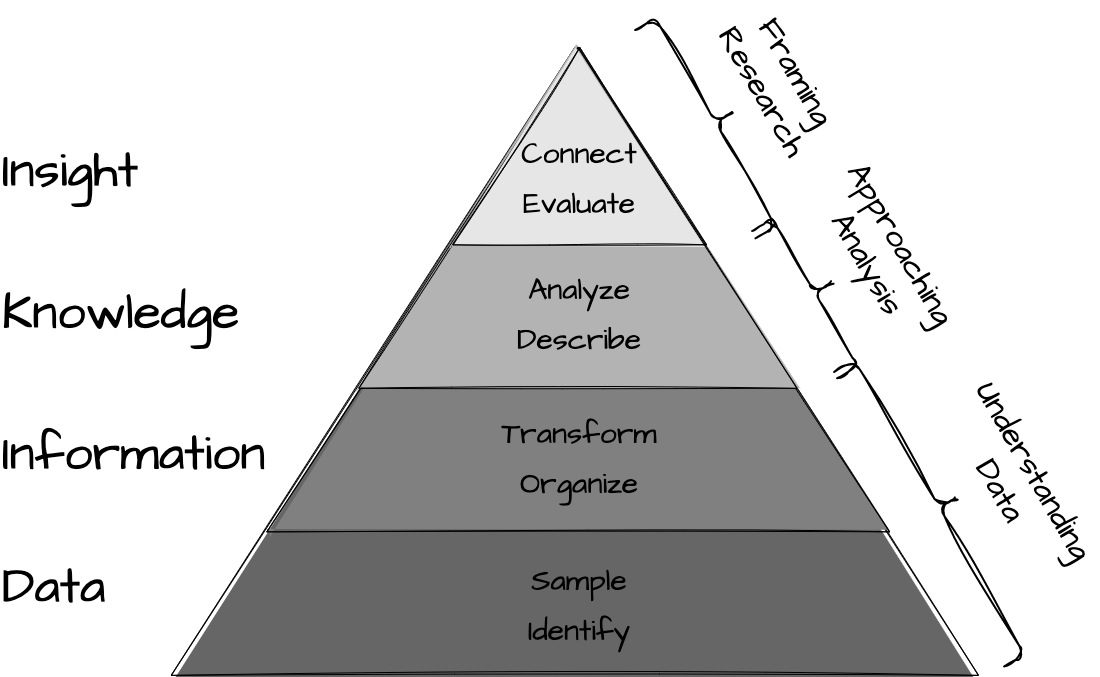
\includegraphics[width=0.75\textwidth,height=\textheight]{figures/framing-research/fr-diki.drawio.png}

}

\caption{\label{fig-fr-visual-summary}Framing research: visual summary}

\end{figure}

This chapter concludes the Foundations part of this textbook. At this
stage our overview of fundamental characteristics of research are in
place to move a project towards implementation, as seen in
Figure~\ref{fig-fr-visual-summary}. From this point forward we will
integrate your conceptual knowledge and emerging R programming skills as
we cover common scenarios encountered when conducting reproducible
research with real-world data.

The next part, Preparation, aims to cover R coding strategies to
acquire, curate, and transform data in preparation for analysis. These
are the first steps in putting a research blueprint into action and by
no coincidence the first components in the Data to Insight Hierarchy.
Without further ado, let's get started!

\hypertarget{activities-2}{%
\section*{Activities}\label{activities-2}}
\addcontentsline{toc}{section}{Activities}

\markright{Activities}

\begin{itemize}
\tightlist
\item[$\square$]
  \faIcon{wrench} Add description of outcomes \ldots{}
\end{itemize}

\begin{tcolorbox}[enhanced jigsaw, rightrule=.15mm, leftrule=.75mm, opacityback=0, arc=.35mm, colback=white, breakable, toprule=.15mm, bottomrule=.15mm, left=2mm]

\textbf{\faIcon{file-code} Recipe}

\textbf{What}:
\href{https://qtalr.github.io/qtalrkit/articles/recipe-4.html}{Project
management}\\
\textbf{How}: Read Recipe 4 and participate in the Hypothes.is online
social annotation.\\
\textbf{Why}: \faIcon{wrench} To learn how to use \ldots{} reproducible
research projects.

\end{tcolorbox}

\begin{tcolorbox}[enhanced jigsaw, rightrule=.15mm, leftrule=.75mm, opacityback=0, arc=.35mm, colback=white, breakable, toprule=.15mm, bottomrule=.15mm, left=2mm]

\textbf{\faIcon{flask} Lab}

\textbf{What}: \href{https://github.com/qtalr/lab-4}{Project
management}\\
\textbf{How}: Clone, fork, and complete the steps in Lab 4.\\
\textbf{Why}: \faIcon{wrench} To \ldots{} a reproducible research
project.

\end{tcolorbox}

\hypertarget{questions-3}{%
\section*{Questions}\label{questions-3}}
\addcontentsline{toc}{section}{Questions}

\markright{Questions}

\begin{tcolorbox}[enhanced jigsaw, rightrule=.15mm, leftrule=.75mm, opacityback=0, arc=.35mm, colback=white, breakable, toprule=.15mm, bottomrule=.15mm, left=2mm]

\textbf{Conceptual questions}

\begin{itemize}
\tightlist
\item
  What are the key characteristics of good research as described in this
  chapter?
\item
  What are some strategies researchers can use to identify potential
  research areas and problems to investigate?
\item
  For each strategy, describe how it contributes to research that is
  purposive, inquisitive, and informed.
\item
  Why is framing a clear, focused research question or hypothesis
  important? Briefly explain how the research question guides the
  overall research process.
\item
  What is the difference between the unit of analysis and the unit of
  observation? How do these concepts relate to the research question?
\item
  What does it mean to operationalize a variable? Why is this important?
\item
  The process of developing a research blueprint involves both
  conceptual planning and practical implementation steps. Explain how
  going through this process not only aids the individual researcher,
  but also the research community.
\item
  Describe the main aspects of developing a research plan.
\item
  Explain why it is important for research to be methodological and
  reproducible. What are some challenges researchers may face in
  achieving this?
\end{itemize}

\end{tcolorbox}

\begin{tcolorbox}[enhanced jigsaw, rightrule=.15mm, leftrule=.75mm, opacityback=0, arc=.35mm, colback=white, breakable, toprule=.15mm, bottomrule=.15mm, left=2mm]

\textbf{\faIcon{wrench} Technical exercises}

\begin{itemize}
\tightlist
\item
  Matching research questions with data sources
\item
  Matching research questions with research plans
\item
  Preregistering a research project (?)
\item
  Propose a quantitative research topic (or question if possible).
  Support your topic with supporting literature. (?)
\item
  \ldots{}
\end{itemize}

\end{tcolorbox}

\part{Preparation}

At this point we begin our journey to implement the research blueprint.
As such, the content will be more focused on the practical steps to
bring a plan to fruition integrating our conceptual understanding of the
research process from the previous chapters with our emerging
programming skills developed in lessons, recipes, and labs.

This part, Preparation, will address data acquistion, curation, and
transformation steps. The goal of data preparation is to create a
dataset which is ready for analysis. In each of these three upcoming
chapters, I will outline some of the main characteristics to consider in
each of these research steps and provide authentic examples of working
with R to implement these steps. In
\protect\hyperlink{sec-acquire-data}{Chapter 5} this includes downloads,
working with APIs, and webscraping. In
\protect\hyperlink{sec-curate-data}{Chapter 6} we turn to organize data
into rectangular, or `tidy', format. Depending on the data or dataset
acquired for the research project, the steps necessary to shape our data
into a base dataset will vary, as we will see. In
\protect\hyperlink{sec-transform-data}{Chapter 7} we will work to
manipulate curated datasets to create datasets which are aligned with
the research aim and research question. This often includes normalizing
values, recoding variables, and generating new variables as well as and
sourcing and merging information from other datasets with the dataset to
be submitted for analysis.

Each of these chapters will cover the necessary documentation to trace
our steps and provide a record of the data preparation process.
Documentation serves to inform the analysis and interpretation of the
results and also forms the cornerstone of reproducible research.

\hypertarget{sec-acquire-data}{%
\chapter{Acquire data}\label{sec-acquire-data}}

\begin{tcolorbox}[enhanced jigsaw, leftrule=.75mm, title=\textcolor{quarto-callout-caution-color}{\faFire}\hspace{0.5em}{Caution}, coltitle=black, opacityback=0, titlerule=0mm, arc=.35mm, bottomtitle=1mm, opacitybacktitle=0.6, colframe=quarto-callout-caution-color-frame, rightrule=.15mm, toptitle=1mm, left=2mm, colback=white, breakable, toprule=.15mm, bottomrule=.15mm, colbacktitle=quarto-callout-caution-color!10!white]

Under development.

\end{tcolorbox}

\begin{quote}
The scariest moment is always just before you start.

―-- Stephen King
\end{quote}

\begin{tcolorbox}[enhanced jigsaw, rightrule=.15mm, leftrule=.75mm, opacityback=0, arc=.35mm, colback=white, breakable, toprule=.15mm, bottomrule=.15mm, left=2mm]

\textbf{\faIcon{list-alt} Outcomes}

\begin{itemize}
\tightlist
\item
  Identify common strategies for acquiring corpus data.
\item
  Describe how to organize and document data acquisition to support
  reproducibility.
\item
  Recall R programming concepts and strategies relevant to acquiring
  data.
\end{itemize}

\end{tcolorbox}

As we start down the path to executing our research blueprint, our first
step is to acquire the primary data that will be employed in the
project. This chapter covers three widely-used strategies for acquiring
corpus data: downloads, APIs (Application Programming Interfaces), and
web scraping. We get started with the most straighforward approaches
from a conceptual standpoint, gradually escalating to more nuanced
methods. We will encounter various file formats and folder structures in
the process and we will address how to effectively organize our data for
subsequent processing. Crucial to our efforts is the process of
documenting our data. We will learn to provide data origin information
to ensure key characteristics of the data and its source are documented.
Along the way we will explore R coding concepts including control
statements and custom functions relevant to the task of acquiring data.
By the end of this chapter, you will not only be adept at acquiring data
from diverse sources but also capable of documenting it comprehensively,
enabling you to replicate the process in the future.

\begin{tcolorbox}[enhanced jigsaw, rightrule=.15mm, leftrule=.75mm, opacityback=0, arc=.35mm, colback=white, breakable, toprule=.15mm, bottomrule=.15mm, left=2mm]

\textbf{\faIcon{terminal} Swirl lesson}

\textbf{What}: \href{https://github.com/qtalr/lessons}{Control
Statements, Custom Functions}\\
\textbf{How}: In the R Console pane load \texttt{swirl}, run
\texttt{swirl()}, and follow prompts to select the lesson.\\
\textbf{Why}: To recognize the logic behind code that can make dynamic
choices and to recall how functions serve to produce efficient,
reusable, and more legible code.

\end{tcolorbox}

\hypertarget{downloads}{%
\section{Downloads}\label{downloads}}

The most common and straightforward method for acquiring corpus data is
through direct downloads. In a nutshell, this method involves navigating
to a website, locating the data, and downloading it to your computing
environment. In some cases access to the data requires manual
intervention and in others the process can be implemented
programmatically. The data may be contained in a single file or multiple
files. The files may be compressed or uncompressed. The data may be
hierarchically organized or not. Each resource will have its own unique
characteristics that will influence the process of acquiring the data.
In this section we will work through a few examples to demonstrate the
general process of acquiring data through downloads.

\hypertarget{manual}{%
\subsection{Manual}\label{manual}}

In contrast to the other data acquisition methods we will cover in this
chapter, \textbf{manual downloads} require human intervention. This
means that manual downloads are non-reproducible in a strict sense and
require that we keep track of and document our procedure. It is a very
common for research projects to acquire data through manual downloads as
many data resources require some legwork before they are accessible for
downloading. These can be resources that require institutional or
private licensing and fees (\href{https://www.ldc.upenn.edu/}{Language
Data Consortium}, \href{http://ice-corpora.net/ice/}{International
Corpus of English}, \href{https://www.corpusdata.org/}{BYU Corpora},
\emph{etc.}), require authorization/ registration
(\href{https://archive.mpi.nl/tla/}{The Language Archive},
\href{https://www.webcorpora.org/}{COW Corpora}, \emph{etc.}), and/ or
are only accessible via resource search interfaces
(\href{https://cesa.arizona.edu/}{Corpus of Spanish in Southern
Arizona}, \href{http://cedel2.learnercorpora.com/}{Corpus Escrito del
Español como L2 (CEDEL2)}, \emph{etc.}).

Let's take a look at how to acquire data from a resource that requires
manual intervention. The resource we will use is the
\href{http://cedel2.learnercorpora.com/}{Corpus Escrito del Español como
L2 (CEDEL2)} (\protect\hyperlink{ref-Lozano2009}{Lozano 2009}), a corpus
of Spanish learner writing. It includes L2 writing from students with a
variety of L1 backgrounds. For comparative puposes it also includes
native writing for Spanish, English, and several other languages.

The CEDEL2 corpus is a freely available resource, but to access the data
you must first use a search interface to select the relevant
characteristics of the data of interest. Following the search/ download
link you can find a search interface that allows the user to select the
subcorpus and filter the results by a set of attributes, seen in
Figure~\ref{fig-ad-cedel2-search}.

\begin{figure}[H]

{\centering 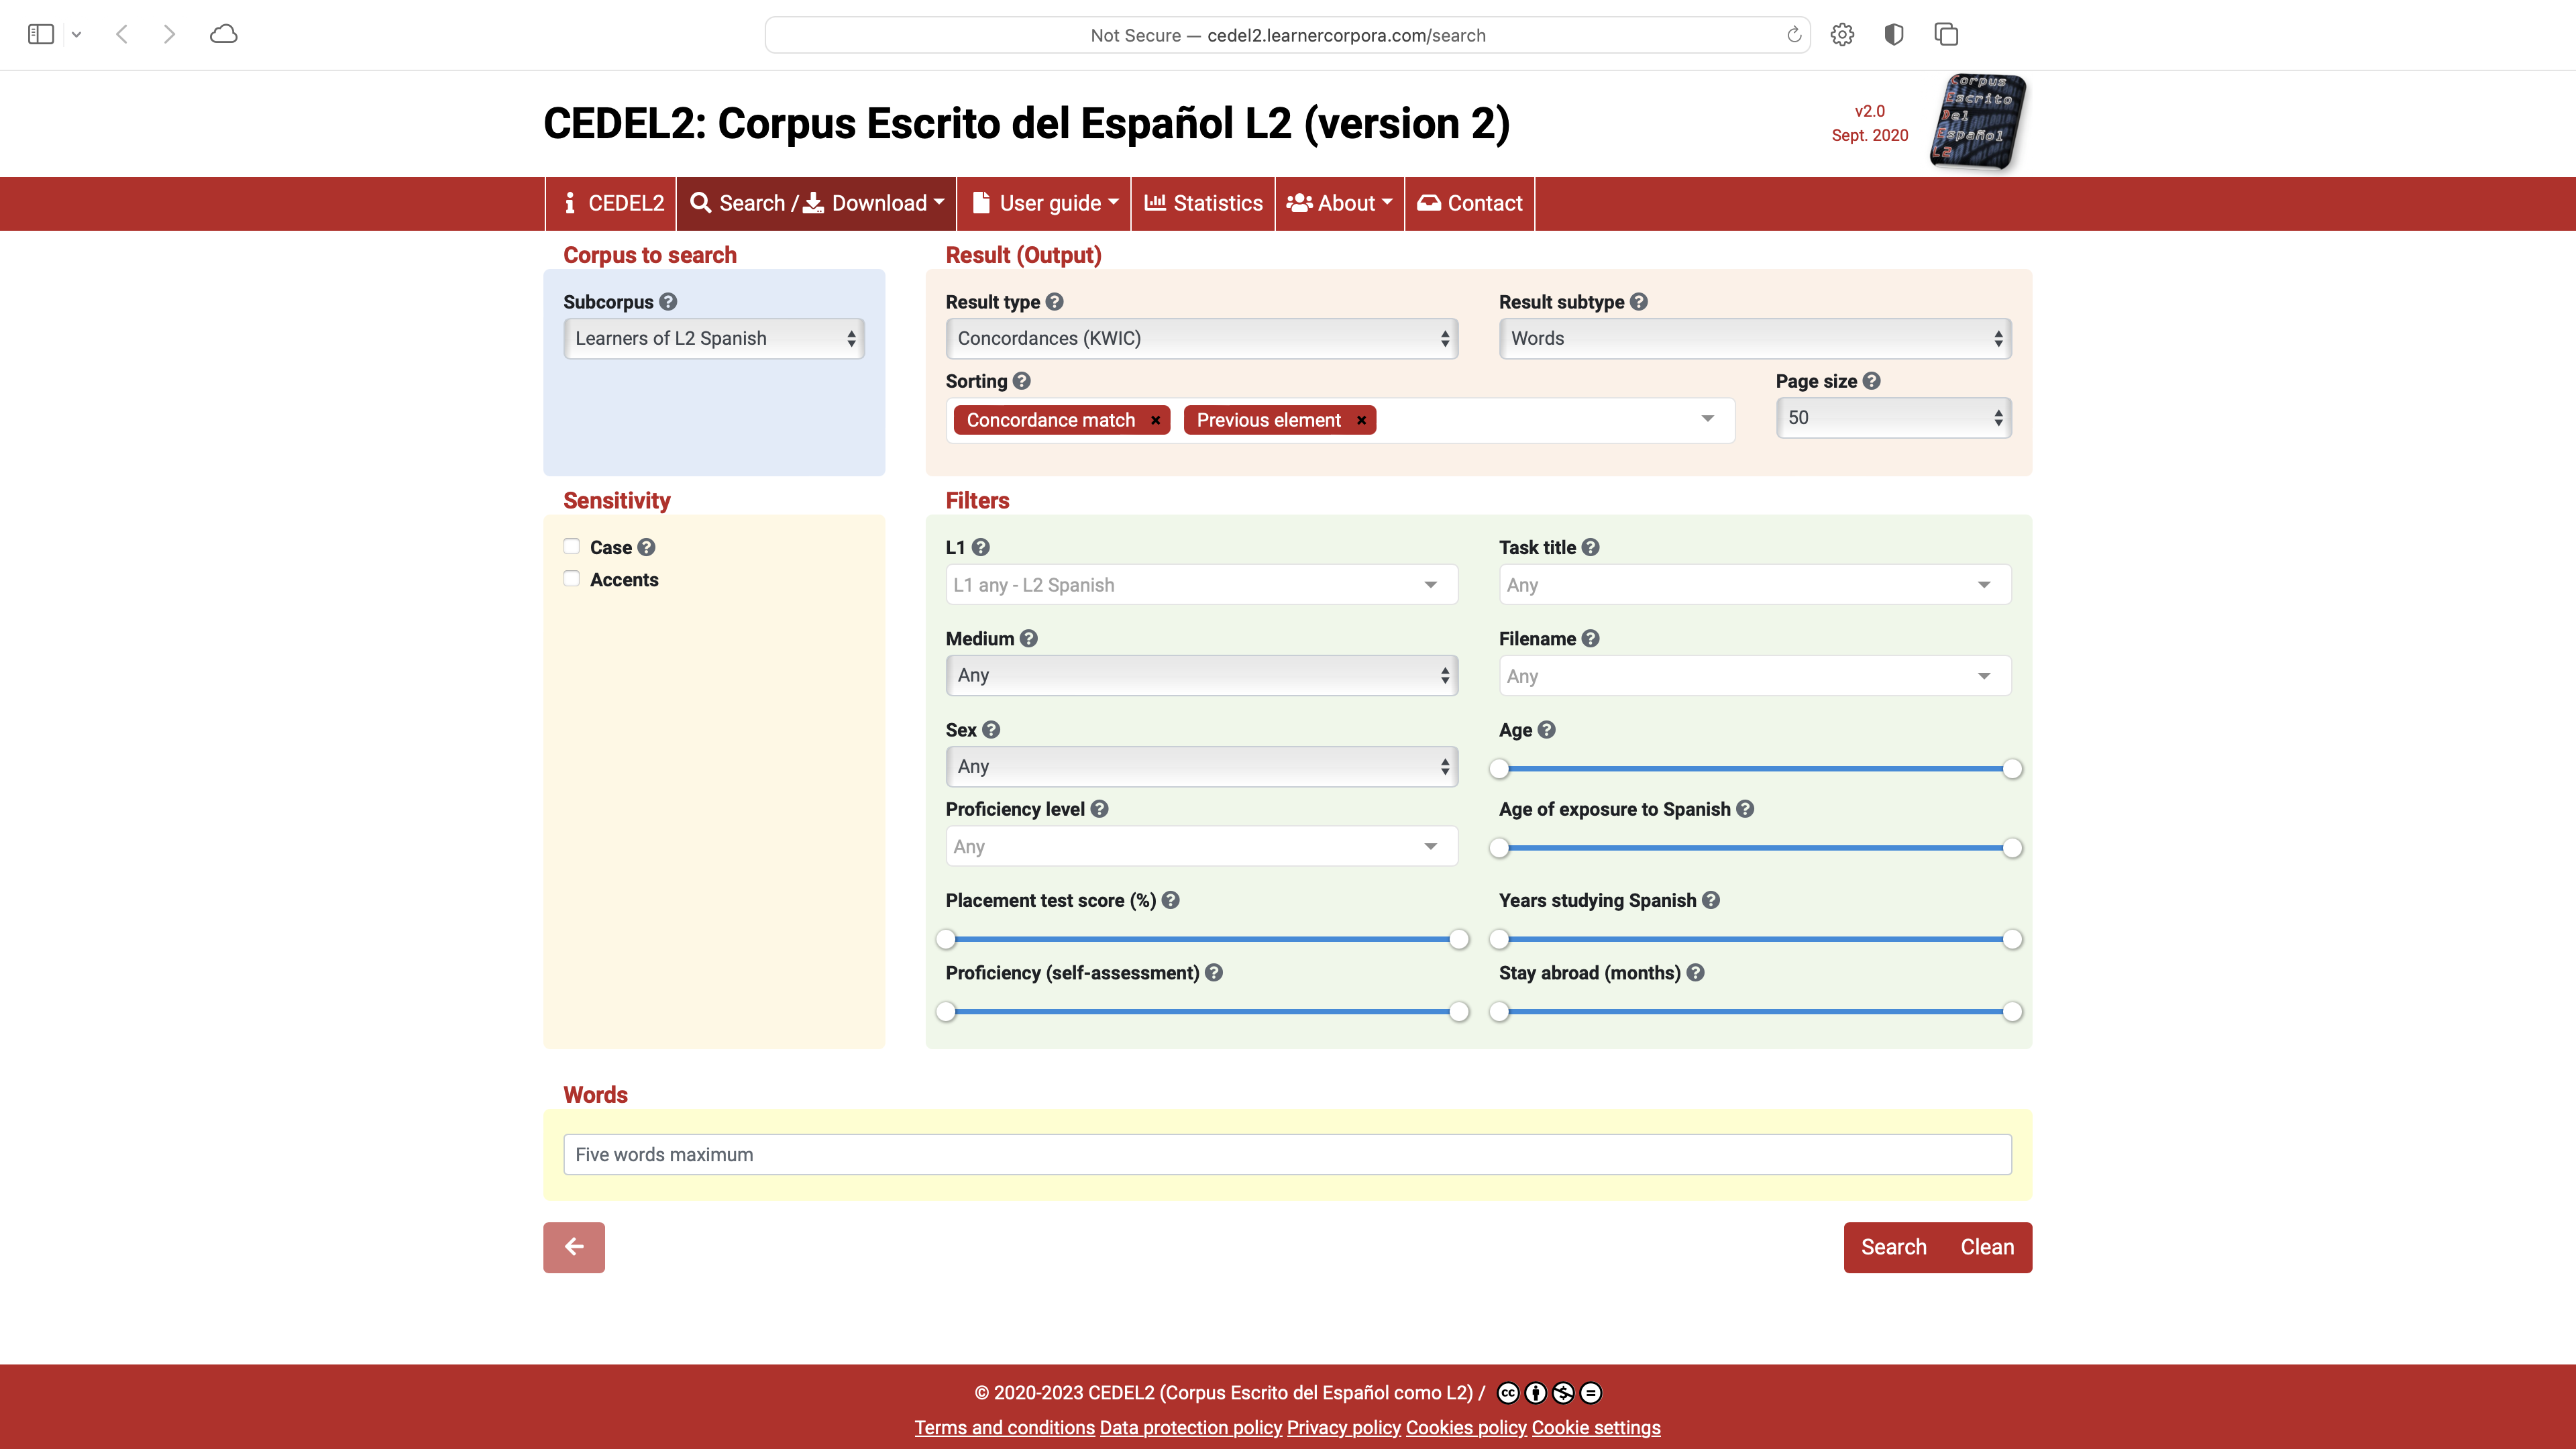
\includegraphics[width=1\textwidth,height=\textheight]{figures/acquire-data/ad-cedel2-search.png}

}

\caption{\label{fig-ad-cedel2-search}Search and download interface for
the CEDEL2 Corpus}

\end{figure}

For this example let's assume that we want to acquire data to use in a
study comparing the use of the Spanish preterite and imperfect past
tense aspect in written texts by English L1 learners of Spanish to
native Spanish speakers. To acquire data for such a project, we will
first select the subcorpus ``Learners of L2 Spanish''. We will set the
results to provide full texts and filter the results to ``L1 English -
L2 Spanish''. Additionally, we will set the medium to ``Written''. This
will provide us with a set of texts for the L2 learners that we can use
for our study. The search parameters and results are shown in
Figure~\ref{fig-ad-cedel2-results}.

\begin{figure}[H]

{\centering 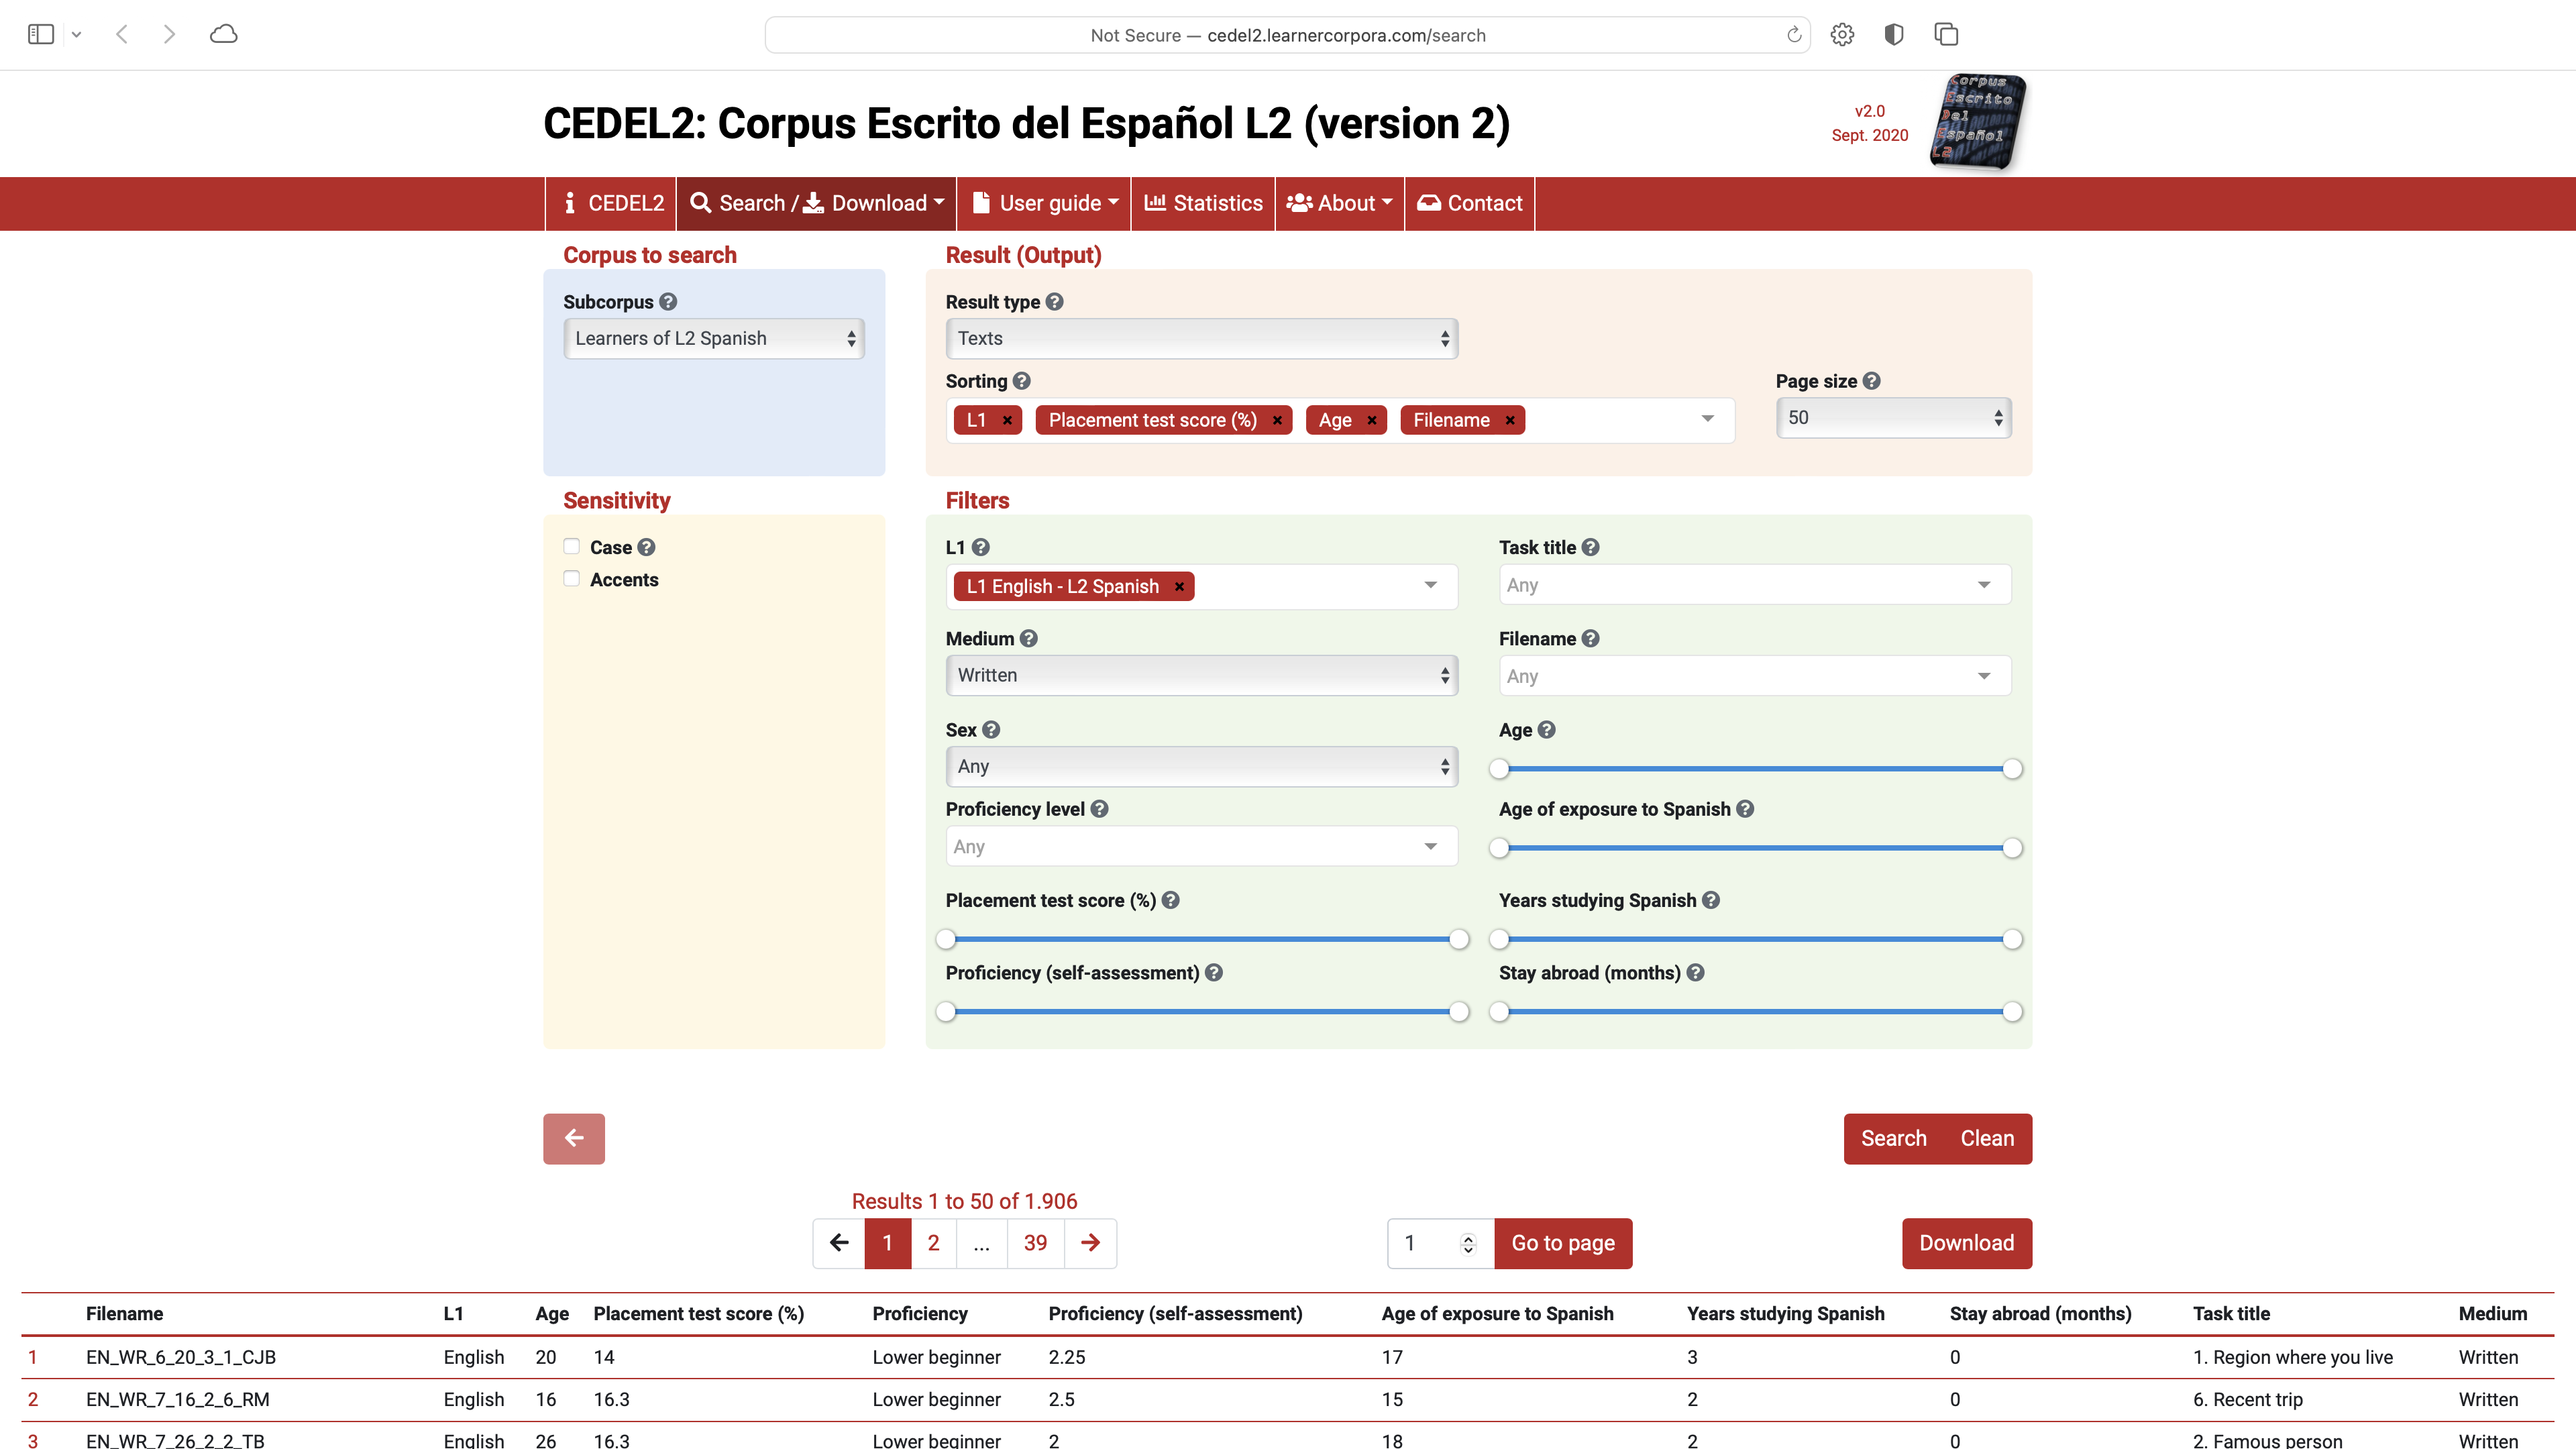
\includegraphics[width=1\textwidth,height=\textheight]{figures/acquire-data/ad-cedel2-results.png}

}

\caption{\label{fig-ad-cedel2-results}Search results for the CEDEL2
Corpus}

\end{figure}

The `Download' link now appears for this search criteria. Following this
link will provide the user a form to fill out. This particular resource
allows for access to different formats to download (Texts only, Texts
with metadata, CSV (Excel), CSV (Others)). I will select the `CSV
(Others)' option so that the data is structured for easier processing
downstream when we work to curate the data in our next processing step.
Then I will choose to save the CSV in the \emph{data/original/}
directory of my project and create a sub-directory named \emph{cedel2/},
as seen in Example~\ref{exm-ad-cedel2-learners-download}.

\begin{example}[]\protect\hypertarget{exm-ad-cedel2-learners-download}{}\label{exm-ad-cedel2-learners-download}

Download CEDEL2 L2 Spanish Learners data

\begin{Shaded}
\begin{Highlighting}[]
\ExtensionTok{data/}
\ExtensionTok{├──}\NormalTok{ analysis/}
\ExtensionTok{├──}\NormalTok{ derived/}
\ExtensionTok{└──}\NormalTok{ original/}
    \ExtensionTok{└──}\NormalTok{ cedel2/}
       \ExtensionTok{└──}\NormalTok{ cedel2{-}l1{-}english{-}learners.csv}
\end{Highlighting}
\end{Shaded}

\end{example}

Note that the file is named \emph{cedel2-l1-english-learners.csv} to
reflect the search criteria used to acquire the data. In combination
with other data documentation, this will help us to maintain
transparency.

Now, after downloading the L2 learner and the native speaker data into
the appropriate directory, we move on to the next processing step,
right? Not so fast! Imagine we are working on a project with a
collaborator. How will they know where the data came from? What if we
need to come back to this data in the future? How will we know what
characteristics we used to filter the data? The directory and filenames
may not be enough. To address these questions we need to document the
origin of the data, and in the case of data acquired through manual
downloads, we need to document the procedures we took to acquire the
data to the best of our ability.

As discussed in Section~\ref{sec-ud-data-origin}, all acquired data
should be accompanied by a data origin file. The majority of this
information can typically be identified on the resource's website and/
or the resource's documentation. In the case of the CEDEL2 corpus, the
corpus homepage provides most of the information we need.

Structurally, data documentation files should be stored close to the
data they describe. So for our data origin file this means adding it to
the \emph{data/original/} directory. Naming the file in a transparent
way is also important. I've named the file \emph{cedel2\_do.csv} to
reflect the name of the corpus, the meaning of the file as data origin
with *\_do\emph{, and the file extension }.csv* to reflect the file
format. CSV files reflect tabular content. It is not required that data
origin files are tabular, but it makes it easier to read and display
them in literate programming documents.

\begin{tcolorbox}[enhanced jigsaw, rightrule=.15mm, leftrule=.75mm, opacityback=0, arc=.35mm, colback=white, breakable, toprule=.15mm, bottomrule=.15mm, left=2mm]

\textbf{\faIcon{hand-point-up} Tip}

There are many ways to create and edit CSV files. You can use a
spreadsheet program like MS Excel or Google Sheets, a text editor like
Notepad or TextEdit, or a code editor like RStudio or VS Code. The
\texttt{qtalrkit} package provides a convenient function,
\texttt{create\_data\_origin()} to create a CSV file with the data
origin boilerplate structure. This CSV file then can be edited to add
the relevant information in any of the above mentioned programs.

Using a spreadsheet program is the easiest method for editing tabular
data. The key is to save the file as a CSV file, and not as an Excel
file, to maintain our adherence to the principle of using open formats
for reproducible research.

\end{tcolorbox}

In Table~\ref{tbl-ad-cedel2-do}, I've created a data origin file for the
CEDEL2 corpus.

\hypertarget{tbl-ad-cedel2-do}{}
\begin{table}
\caption{\label{tbl-ad-cedel2-do}Data origin file for the CEDEL2 corpus }\tabularnewline

\centering
\begin{tabular}{ll}
\toprule
attribute & description\\
\midrule
Resource name & CEDEL2: Corpus Escrito del Español como L2.\\
Data source & http://cedel2.learnercorpora.com/, https://doi.org/10.1177/02676583211050522\\
Data sampling frame & Corpus that contains samples of the language produced from learners of Spanish as a second language. For comparative purposes, it also contains a native control subcorpus of the language produced by native speakers of Spanish from different varieties (peninsular Spanish and all varieties of Latin American Spanish), so it can be used as a native corpus in its own right.\\
Data collection date(s) & 2006-2020.\\
Data format & CSV file. Each row corresponds to a writing sample. Each column is an attribute of the writing sample.\\
\addlinespace
Data schema & A CSV file for L2 learners and a CSV file for native speakers.\\
License & CC BY-NC-ND 3.0 ES\\
Attribution & Lozano, C. (2022). CEDEL2: Design, compilation and web interface of an online corpus for L2 Spanish acquisition research. Second Language Research, 38(4), 965-983. https://doi.org/10.1177/02676583211050522.\\
\bottomrule
\end{tabular}
\end{table}

Given this is a manual download we also need to document the procedure
used to retrieve the data in prose. The script in the \emph{code/}
directory that is typically used to acquire the data is not used to
programmatically retrieve data in this case. However, to keep things
predictable we will use this file to document the download procedure.
I've created a Quarto file named \emph{1\_acquire\_data.qmd} in the
\emph{code/} directory of my project.

A glimpse at the directory structure of the project at this point is
seen in Example~\ref{exm-ad-cedel2-structure}.

\begin{example}[]\protect\hypertarget{exm-ad-cedel2-structure}{}\label{exm-ad-cedel2-structure}

Project structure for the CEDEL2 corpus data acquisition

\begin{Shaded}
\begin{Highlighting}[]
\ExtensionTok{project/}
\ExtensionTok{├──}\NormalTok{ code/}
\ExtensionTok{│}\NormalTok{   ├── 1\_acquire\_data.qmd}
\ExtensionTok{│}\NormalTok{   └── ...}
\ExtensionTok{├──}\NormalTok{ data/}
\ExtensionTok{│}\NormalTok{   ├── analysis/}
\ExtensionTok{│}\NormalTok{   ├── derived/}
\ExtensionTok{│}\NormalTok{   └── original/}
\ExtensionTok{│}\NormalTok{       ├── cedel2\_do.csv}
\ExtensionTok{│}\NormalTok{       └── cedel2/}
\KeywordTok{|}           \ExtensionTok{├──}\NormalTok{ cedel2{-}l1{-}english{-}learners.csv}
\KeywordTok{|}           \ExtensionTok{└──}\NormalTok{ cedel2{-}native{-}spanish{-}speakers.csv}
\ExtensionTok{├──}\NormalTok{ output/}
\ExtensionTok{│}\NormalTok{   ├── figures/}
\ExtensionTok{│}\NormalTok{   ├── reports/}
\ExtensionTok{│}\NormalTok{   ├── results/}
\ExtensionTok{│}\NormalTok{   └── tables/}
\ExtensionTok{├──}\NormalTok{ README.md}
\ExtensionTok{└──}\NormalTok{ \_main.R}
\end{Highlighting}
\end{Shaded}

\end{example}

In the \emph{1\_acquire\_data.qmd} file I've added example sections to
display the data origin CSV file as a table and to document the data
download procedures, as seen in
File~\ref{lst-ad-cedel2-acquire-data-qmd}.

\begin{codelisting}

\caption{\texttt{1-acquire-data.qmd}: Acquire data file}

\hypertarget{lst-ad-cedel2-acquire-data-qmd}{%
\label{lst-ad-cedel2-acquire-data-qmd}}%
\begin{Shaded}
\begin{Highlighting}[]
\CommentTok{{-}{-}{-}}
\AnnotationTok{title:}\CommentTok{ "Acquire data"}
\AnnotationTok{format:}\CommentTok{ html}
\CommentTok{{-}{-}{-}}
\FunctionTok{\#\# Overview  }
\NormalTok{The goal of this script is to acquire and document data for this project from the CEDEL2 corpus. The acquired data will be stored in the }\InformationTok{\textasciigrave{}data/original/cedel2/\textasciigrave{}}\NormalTok{ directory.}
\FunctionTok{\#\# Data origin  }

\NormalTok{To document the origin of the data we created a file named }\InformationTok{\textasciigrave{}cedel2\_do.csv\textasciigrave{}}\NormalTok{ in the }\InformationTok{\textasciigrave{}data/original/\textasciigrave{}}\NormalTok{ directory. This file contains the following information: }

\InformationTok{\textasciigrave{}\textasciigrave{}\textasciigrave{}\{r\}}
\CommentTok{\#| label: tbl{-}cedel2{-}data{-}origin}
\CommentTok{\#| tbl{-}cap: "Data origin file for the CEDEL2 corpus"}
\CommentTok{\#| echo: false}

\CommentTok{\# Display data origin file}
\NormalTok{readr}\SpecialCharTok{::}\FunctionTok{read\_csv}\NormalTok{(}\StringTok{"../data/original/cedel2\_do.csv"}\NormalTok{) }\SpecialCharTok{|\textgreater{}} 
\NormalTok{  knitr}\SpecialCharTok{::}\FunctionTok{kable}\NormalTok{()}
\InformationTok{\textasciigrave{}\textasciigrave{}\textasciigrave{}}
\FunctionTok{\#\# Download procedures  }
\NormalTok{The process to acquire data from the CEDEL2 corpus involved the following steps:}

\NormalTok{L2 Spanish Learners:  }
\SpecialStringTok{1. }\NormalTok{Navigate to the }\CommentTok{[}\OtherTok{CEDEL2 Corpus}\CommentTok{](http://cedel2.learnercorpora.com/search)}\NormalTok{ search interface}
\SpecialStringTok{2. }\NormalTok{Select the subcorpus "Learners of L2 Spanish"}
\SpecialStringTok{3. }\NormalTok{Set the results to provide full texts}
\SpecialStringTok{4. }\NormalTok{Filter the results to "L1 English {-} L2 Spanish"}
\SpecialStringTok{5. }\NormalTok{Set the medium to "Written"}
\SpecialStringTok{6. }\NormalTok{Download the data in CSV format}
\SpecialStringTok{7. }\NormalTok{Save the CSV file to the }\InformationTok{\textasciigrave{}data/original/cedel2/\textasciigrave{}}\NormalTok{ directory as }\InformationTok{\textasciigrave{}cedel2{-}l1{-}english{-}learners.csv\textasciigrave{}}

\NormalTok{Spanish natives: }
\end{Highlighting}
\end{Shaded}

\end{codelisting}

The output from \emph{1\_acquire\_data.qmd} will contain a table
displaying the data origin file and a prose section documenting the data
acquisition process. This will provide a transparent record of the data
acquisition process for future reference.

Manually downloading other resources will inevitably include unique
processes for obtaining the data, but in the end the data should be
archived in the research structure in the \emph{data/original/}
directory and documented in the appropriate places. The acquired data is
treated as `read-only', meaning it is not modified in any way. This
gives us a transparent starting point for subsequent steps in the data
preparation process.

\hypertarget{programmatic}{%
\subsection{Programmatic}\label{programmatic}}

There are many resources that provide corpus data that is directly
accessible for which programmatic downloads can be applied. A
\textbf{programmatic download} is a download in which the process can be
automated through code. Thus, this is a reproducible process. The data
can be acquired by anyone with access to the necessary code.

In this case, and subsquent data acquisition procedures in this chapter,
we use the \emph{1\_acquire\_data.qmd} Quarto file to its full potential
intermingling prose, code, and code comments to execute and document the
download procedure. In File~\ref{lst-ad-swda-acquire-data-qmd}, I've
added example sections to display example boilerplate structure for a
programmatic data acquisition and documentation.

\begin{codelisting}

\caption{\texttt{1-acquire-data.qmd}: Acquire data file}

\hypertarget{lst-ad-swda-acquire-data-qmd}{%
\label{lst-ad-swda-acquire-data-qmd}}%
\begin{Shaded}
\begin{Highlighting}[]
\CommentTok{{-}{-}{-}}
\AnnotationTok{title:}\CommentTok{ "Acquire data"}
\AnnotationTok{format:}\CommentTok{ html}
\CommentTok{{-}{-}{-}}

\FunctionTok{\#\# Overview}

\NormalTok{The goal of this script is to ...}

\FunctionTok{\#\# Data origin}

\NormalTok{To document the origin of the data we created a file named ...}

\FunctionTok{\#\# Download procedures}

\InformationTok{\textasciigrave{}\textasciigrave{}\textasciigrave{}\{r\}}
\CommentTok{\#| label: setup}

\CommentTok{\# Load libraries}
\FunctionTok{library}\NormalTok{(tidyverse)}
\InformationTok{\textasciigrave{}\textasciigrave{}\textasciigrave{}}
\InformationTok{\textasciigrave{}\textasciigrave{}\textasciigrave{}\{r\}}
\CommentTok{\# .. additional code here to acquire data ...}
\InformationTok{\textasciigrave{}\textasciigrave{}\textasciigrave{}}
\NormalTok{... and so on}
\end{Highlighting}
\end{Shaded}

\end{codelisting}

To illustrate how this works to conduct a programmatic download, we will
work with the Switchboard Dialog Act Corpus (SWDA)
(\protect\hyperlink{ref-SWDA2008}{University of Colorado Boulder 2008}).
The version that we will use is found on the Linguistic Data Consortium
under the \href{https://catalog.ldc.upenn.edu/LDC97S62}{Switchboard-1
Release 2 Corpus}. The corpus and related documentation are linked on
the catalog page \url{https://catalog.ldc.upenn.edu/docs/LDC97S62/}.

From the documentation we learn that the corpus contains transcripts for
1155 5-minute two-way telephone conversations among English speakers for
all areas of the United States. The speakers were given a topic to
discuss and the conversations were recorded. The corpus metadata and
annotations for sociolinguistic and discourse features.

The SWDA was referred to in Section~\ref{sec-aa-infer} to support our
toy hypothesis that men and women differ in the frequency of the use of
questions in spontaneous conversations. This corpus, as you can image,
could support a wide range of interesting reseach questions. Let's
assume we are following research conducted by Tottie
(\protect\hyperlink{ref-Tottie2011}{2011}) to explore the use of filled
pauses such as ``um'' and ``uh'' and traditional sociolinguistic
variables such as sex, age, and education in spontaneous speech by
American English speakers.

With this goal in mind, let's get started writing the code to download
and organize the data in our project directory. First we need to
identify the URL (Uniform Resource Locator) for the data that we want to
download. More often than not this file will be some type of compressed
archive file with an extension such as \emph{.zip} (Zipped file),
\emph{.tar} (Tarball file), or \emph{tar.gz} (Gzipped tarball file),
which is the case for the SWDA corpus. Compressed files make downloading
multiple files easy by grouping files and directories into one file.

\begin{tcolorbox}[enhanced jigsaw, rightrule=.15mm, leftrule=.75mm, opacityback=0, arc=.35mm, colback=white, breakable, toprule=.15mm, bottomrule=.15mm, left=2mm]

\textbf{\faIcon{lightbulb} Consider this}

You may be wondering what the difference betwen \emph{.zip},
\emph{.tar}, and \emph{.tar.gz} files are. The \emph{.zip} file format
is the most common. It groups file and directories into one file
(archives) and compresses them to reduce the size of the file in one
step when the file is created.

The \emph{.tar} file format is used archive files and folders, it does
not perform compression. Gzipping peforms the compression to the
\emph{.tar} file resulting in a file with the \emph{.tar.gz} extension.
Notably the \emph{.gz} compression is highly efficient for large files.
Take the \emph{swda.tar.gz} file for example. It has a compressed file
size of 4.6 MB, but when uncompressed it is 16.9 MB. This is a 73\%
reduction in file size.

\end{tcolorbox}

In R we can use the \texttt{download.file()} function from base R. The
\texttt{download.file()} function minimally requires two arguments:
\texttt{url} and \texttt{destfile}. These correspond to the file to
download and the location where it is to be saved to disk. To break out
the process a bit, I will assign the URL and destination file path to
variables and then use the \texttt{download.file()} function to download
the file.

\begin{example}[]\protect\hypertarget{exm-ad-swda-download-file}{}\label{exm-ad-swda-download-file}

~

\begin{Shaded}
\begin{Highlighting}[]
\CommentTok{\# URL to SWDA corpus compressed file}
\NormalTok{file\_url }\OtherTok{\textless{}{-}} 
  \StringTok{"https://catalog.ldc.upenn.edu/docs/LDC97S62/swb1\_dialogact\_annot.tar.gz"}

\CommentTok{\# Relative path to project/data/original directory}
\NormalTok{file\_path }\OtherTok{\textless{}{-}} \StringTok{"../data/original/swda.tar.gz"}

\CommentTok{\# Download SWDA corpus compressed file}
\FunctionTok{download.file}\NormalTok{(}\AttributeTok{url =}\NormalTok{ file\_url, }\AttributeTok{destfile =}\NormalTok{ file\_path)}
\end{Highlighting}
\end{Shaded}

\end{example}

\begin{tcolorbox}[enhanced jigsaw, rightrule=.15mm, leftrule=.75mm, opacityback=0, arc=.35mm, colback=white, breakable, toprule=.15mm, bottomrule=.15mm, left=2mm]

\textbf{\faIcon{exclamation-triangle} Warning}

Note that the \texttt{file\_path} variable in
Example~\ref{exm-ad-swda-download-file} is a relative path to the
\emph{data/original/} directory. This is because the
\emph{1\_acquire\_data.qmd} file that we are using for this code is
located in the \emph{code/} directory and the \emph{data/} directory is
a sibling directory to the \emph{code/} directory.

It is also possible to use an absolute path to the \emph{data/original/}
directory. I will have more to say about the advantages and
disadvantages of relative and absolute paths in reproducible research in
Chapter~\ref{sec-collaboration}.

\end{tcolorbox}

As we can see looking at the directory structure, in
Example~\ref{exm-ad-swda-download-location}, the \emph{swda.tar.zip}
file has been added to the \emph{data/original/} directory.

\begin{example}[]\protect\hypertarget{exm-ad-swda-download-location}{}\label{exm-ad-swda-download-location}

Downloaded SWDA corpus compressed file

\begin{Shaded}
\begin{Highlighting}[]
\ExtensionTok{data/}
\ExtensionTok{├──}\NormalTok{ analysis/}
\ExtensionTok{├──}\NormalTok{ derived/}
\ExtensionTok{└──}\NormalTok{ original/}
    \ExtensionTok{└──}\NormalTok{ swda.tar.zip}
\end{Highlighting}
\end{Shaded}

\end{example}

Once an compressed file is downloaded, however, the file needs to be
`decompressed' to reveal the directory structure and files. To
decompress this \emph{.tar.gz} file we use the \texttt{untar()} function
with the arguments \texttt{tarfile} pointing to the \emph{.tar.gz} file
and \texttt{exdir} specifying the directory where we want the files to
be extracted to. Again, I will assign the arguments to variables. Then
we can decompress the file using the \texttt{untar()} function.

\begin{example}[]\protect\hypertarget{exm-ad-swda-decompress-file}{}\label{exm-ad-swda-decompress-file}

~

\begin{Shaded}
\begin{Highlighting}[]
\CommentTok{\# Relative path to the compressed file}
\NormalTok{tar\_file }\OtherTok{\textless{}{-}} \StringTok{"../data/original/swda.tar.gz"}

\CommentTok{\# Relative path to the directory to extract to}
\NormalTok{extract\_to\_dir }\OtherTok{\textless{}{-}} \StringTok{"../data/original/swda/"}

\CommentTok{\# Decompress .zip file and extract to our target directory}
\FunctionTok{untar}\NormalTok{(tar\_file, extract\_to\_dir)}
\end{Highlighting}
\end{Shaded}

\end{example}

The directory structure of \emph{data/} in
Example~\ref{exm-ad-swda-decompress-location} now shows the
\emph{swda.tar.gz} file and the \emph{swda} directory that contains the
decompressed directories and files.

\begin{example}[]\protect\hypertarget{exm-ad-swda-decompress-location}{}\label{exm-ad-swda-decompress-location}

~

\begin{Shaded}
\begin{Highlighting}[]
\ExtensionTok{data/}
\ExtensionTok{├──}\NormalTok{ analysis/}
\ExtensionTok{├──}\NormalTok{ derived/}
\ExtensionTok{└──}\NormalTok{ original/}
    \ExtensionTok{├──}\NormalTok{ swda/}
    \ExtensionTok{│}\NormalTok{   ├── README}
    \ExtensionTok{│}\NormalTok{   ├── doc/}
    \ExtensionTok{│}\NormalTok{   ├── sw00utt/}
    \ExtensionTok{│}\NormalTok{   ├── sw01utt/}
    \ExtensionTok{│}\NormalTok{   ├── sw02utt/}
    \ExtensionTok{│}\NormalTok{   ├── sw03utt/}
    \ExtensionTok{│}\NormalTok{   ├── sw04utt/}
    \ExtensionTok{│}\NormalTok{   ├── sw05utt/}
    \ExtensionTok{│}\NormalTok{   ├── sw06utt/}
    \ExtensionTok{│}\NormalTok{   ├── sw07utt/}
    \ExtensionTok{│}\NormalTok{   ├── sw08utt/}
    \ExtensionTok{│}\NormalTok{   ├── sw09utt/}
    \ExtensionTok{│}\NormalTok{   ├── sw10utt/}
    \ExtensionTok{│}\NormalTok{   ├── sw11utt/}
    \ExtensionTok{│}\NormalTok{   ├── sw12utt/}
    \ExtensionTok{│}\NormalTok{   └── sw13utt/}
    \ExtensionTok{└──}\NormalTok{ swda.tar.gz}
\end{Highlighting}
\end{Shaded}

\end{example}

At this point we have acquired the data programmatically and with this
code as part of our workflow anyone could run this code and reproduce
the same results. The code as it is, however, is not ideally efficient.
Firstly the \emph{swda.tar.gz} file is not strictly needed after we
decompress it and it occupies disk space if we keep it. And second, each
time we run this code the file will be downloaded from the remote
server. This leads to unnecessary data transfer and server traffic and
will overwrite the data if it already exists in our project directory
which could be problematic if the data changes on the remote server.
Let's tackle each of these issues in turn.

To avoid writing the \emph{swda.tar.gz} file to disk (long-term) we can
use the \texttt{tempfile()} function to open a temporary holding space
for the file in the computing environment. This space can then be used
to store the file, decompress it, and then the temporary file will
automatically be deleted. We assign the temporary space to an R object
we will name \texttt{temp\_file} with the \texttt{tempfile()} function.
This object can now be used as the value of the argument
\texttt{destfile} in the \texttt{download.file()} function.

\begin{example}[]\protect\hypertarget{exm-ad-swda-temp-file}{}\label{exm-ad-swda-temp-file}

~

\begin{Shaded}
\begin{Highlighting}[]
\CommentTok{\# URL to SWDA corpus compressed file}
\NormalTok{file\_url }\OtherTok{\textless{}{-}} 
  \StringTok{"https://catalog.ldc.upenn.edu/docs/LDC97S62/swb1\_dialogact\_annot.tar.gz"}

\CommentTok{\# Create a temporary file space for our .tar.gz file}
\NormalTok{temp\_file }\OtherTok{\textless{}{-}} \FunctionTok{tempfile}\NormalTok{()}

\CommentTok{\# Download SWDA corpus compressed file}
\FunctionTok{download.file}\NormalTok{(file\_url, temp\_file)}
\end{Highlighting}
\end{Shaded}

\end{example}

\begin{tcolorbox}[enhanced jigsaw, rightrule=.15mm, leftrule=.75mm, opacityback=0, arc=.35mm, colback=white, breakable, toprule=.15mm, bottomrule=.15mm, left=2mm]

\textbf{\faIcon{hand-point-up} Tip}

In Example~\ref{exm-ad-swda-temp-file}, I've used the values stored in
the objects \texttt{file\_url} and \texttt{temp\_file} in the
\texttt{download.file()} function without specifying the argument names
--only providing the names of the objects. R will assume that values of
a function map to the ordering of the arguments. If your values do not
map to ordering of the arguments you are required to specify the
argument name and the value. To view the ordering of objects hit
\texttt{tab} after entering the function name or consult the function
documentation by prefixing the function name with \texttt{?} and hitting
\texttt{enter}.

\end{tcolorbox}

At this point our downloaded file is stored temporarily on disk and can
be accessed and decompressed to our target directory using
\emph{temp\_file} as the value for the argument \texttt{tarfile} from
the \texttt{untar()} function. I've assigned our target directory path
to \texttt{extract\_to\_dir} and used it as the value for the argument
\texttt{exdir}.

\begin{example}[]\protect\hypertarget{exm-ad-swda-untar-temp}{}\label{exm-ad-swda-untar-temp}

~

\begin{Shaded}
\begin{Highlighting}[]
\CommentTok{\# Assign our target directory to \textasciigrave{}extract\_to\_dir\textasciigrave{}}
\NormalTok{extract\_to\_dir }\OtherTok{\textless{}{-}} \StringTok{"../data/original/swda/"}

\CommentTok{\# Decompress .tar.gz file and extract to our target directory}
\FunctionTok{untar}\NormalTok{(}\AttributeTok{tarfile =}\NormalTok{ temp\_file, }\AttributeTok{exdir =}\NormalTok{ target\_dir)}
\end{Highlighting}
\end{Shaded}

\end{example}

Our directory structure in Example~\ref{exm-ad-swda-untar-temp} is the
same as in Example~\ref{exm-ad-swda-decompress-location}, minus the
\emph{swda.tar.gz} file.

The second issue I raised concerns the fact that running this code as
part of our project will repeat the download each time. Since we would
like to be good citizens and avoid unnecessary traffic on the web and
avoid potential issues in overwriting data, it would be nice if our code
checked to see if we already have the data on disk and if it exists,
then skip the download, if not then download it.

The desired functionality we've described can be implemented using the
\texttt{if()} function. The \texttt{if()} function is one of a class of
functions known as control statements. \textbf{Control statments} allow
us to control the flow of our code by evaluating logical statements and
processing subsequent code based on the logical value it is passed as an
argument.

So in this case we want to evaluate whether the data directory exists on
disk. If it does then skip the download, if not, proceed with the
download. In combination with \texttt{else} which provides the `if not'
part of the statement, we have the following logical flow in
Example~\ref{exm-ad-if-dir-exists}.

\begin{example}[]\protect\hypertarget{exm-ad-if-dir-exists}{}\label{exm-ad-if-dir-exists}

~

\begin{Shaded}
\begin{Highlighting}[]
\ControlFlowTok{if}\NormalTok{ (DIRECTORY\_EXISTS) \{}
  \CommentTok{\# Do nothing}
\NormalTok{\} }\ControlFlowTok{else}\NormalTok{ \{}
  \CommentTok{\# Download data}
\NormalTok{\}}
\end{Highlighting}
\end{Shaded}

\end{example}

We can simplify this statement by using the \texttt{!} operator which
negates the logical value of the statement it precedes. So if the
directory exists, \texttt{!DIRECTORY\_EXISTS} will return \texttt{FALSE}
and if the directory does not exist, \texttt{!DIRECTORY\_EXISTS} will
return \texttt{TRUE}. In other words, if the directory does not exist,
download the data. This is shown in
Example~\ref{exm-ad-if-dir-exists-simplified}.

\begin{example}[]\protect\hypertarget{exm-ad-if-dir-exists-simplified}{}\label{exm-ad-if-dir-exists-simplified}

~

\begin{Shaded}
\begin{Highlighting}[]
\ControlFlowTok{if}\NormalTok{ (}\SpecialCharTok{!}\NormalTok{DIRECTORY\_EXISTS) \{}
  \CommentTok{\# Download data}
\NormalTok{\}}
\end{Highlighting}
\end{Shaded}

\end{example}

Now, to determine if a directory exists in our project directory we will
turn to the \texttt{fs} package (\protect\hyperlink{ref-R-fs}{Hester,
Wickham, and Csárdi 2023}). The \texttt{fs} package provides a set of
functions for interacting with the file system, including
\texttt{dir\_exists()}. \texttt{dir\_exists()} takes a path to a
directory as an argument and returns the logical value, \texttt{TRUE},
if that directory exists, and \texttt{FALSE} if it does not.

We can use this function to evaluate whether the directory exists and
then use the \texttt{if()} function to process the subsequent code based
on the logical flow we set out in
Example~\ref{exm-ad-if-dir-exists-simplified}. Applied to our project,
the code will look like Example~\ref{exm-ad-swda-if-dir-exists}.

\begin{example}[]\protect\hypertarget{exm-ad-swda-if-dir-exists}{}\label{exm-ad-swda-if-dir-exists}

~

\begin{Shaded}
\begin{Highlighting}[]
\CommentTok{\# Load the \textasciigrave{}fs\textasciigrave{} package}
\FunctionTok{library}\NormalTok{(fs)}

\CommentTok{\# URL to SWDA corpus compressed file}
\NormalTok{file\_url }\OtherTok{\textless{}{-}} 
  \StringTok{"https://catalog.ldc.upenn.edu/docs/LDC97S62/swb1\_dialogact\_annot.tar.gz"}

\CommentTok{\# Create a temporary file space for our .tar.gz file}
\NormalTok{temp\_file }\OtherTok{\textless{}{-}} \FunctionTok{tempfile}\NormalTok{()}

\CommentTok{\# Assign our target directory to \textasciigrave{}extract\_to\_dir\textasciigrave{}}
\NormalTok{extract\_to\_dir }\OtherTok{\textless{}{-}} \StringTok{"../data/original/swda/"}

\CommentTok{\# Check if our target directory exists}
\CommentTok{\# If it does not exist, download the file and extract it}
\ControlFlowTok{if}\NormalTok{ (}\SpecialCharTok{!}\FunctionTok{dir\_exists}\NormalTok{(extract\_to\_dir)) \{}
  \CommentTok{\# Download SWDA corpus compressed file}
  \FunctionTok{download.file}\NormalTok{(file\_url, temp\_file)}
  
  \CommentTok{\# Decompress .tar.gz file and extract to our target directory}
  \FunctionTok{untar}\NormalTok{(}\AttributeTok{tarfile =}\NormalTok{ temp\_file, }\AttributeTok{exdir =}\NormalTok{ extract\_to\_dir)}
\NormalTok{\}}
\end{Highlighting}
\end{Shaded}

\end{example}

The code in Example~\ref{exm-ad-swda-if-dir-exists} is added to the
\emph{1\_acquire\_data.qmd} file we introduced in
File~\ref{lst-ad-swda-acquire-data-qmd}. When this file is run, the SWDA
corpus data will be downloaded and extracted to our project directory.
If the data already exists, the download will be skipped, just as we
wanted.

Before we move on, we need to make sure to create and add the
appropriate information to the data origin file. To make this easier,
the \texttt{qtalrkit} package includes a function,
\texttt{create\_data\_origin()}, to create a data origin file template
in CSV format. This function takes the path for the desired file. In the
SWDA Corpus case, this might be something like:
\emph{../data/original/swda\_do.csv}. The function only needs to be run
once and does not need to be part of the reproducible workflow.

Running the code in Example~\ref{exm-ad-swda-create-do} at the console
will create the file. Open it in your preferred text or spreadsheet
editor to add the appropriate information.

\begin{example}[]\protect\hypertarget{exm-ad-swda-create-do}{}\label{exm-ad-swda-create-do}

~

\begin{Shaded}
\begin{Highlighting}[]
\CommentTok{\# Load the \textasciigrave{}qtalrkit\textasciigrave{} package}
\FunctionTok{library}\NormalTok{(qtalrkit)}

\CommentTok{\# Create a data origin file template}
\FunctionTok{create\_data\_origin}\NormalTok{(}\StringTok{"../data/original/swda\_do.csv"}\NormalTok{)}
\end{Highlighting}
\end{Shaded}

\end{example}

Our complete project structure for the SWDA corpus data acquisition is
shown in Example~\ref{exm-ad-swda-structure}.

\begin{example}[]\protect\hypertarget{exm-ad-swda-structure}{}\label{exm-ad-swda-structure}

Project structure for the SWDA corpus data acquisition

\begin{Shaded}
\begin{Highlighting}[]
\ExtensionTok{project/}
\ExtensionTok{├──}\NormalTok{ code/}
\ExtensionTok{│}\NormalTok{   ├── 1\_acquire\_data.qmd}
\ExtensionTok{│}\NormalTok{   └── ...}
\ExtensionTok{├──}\NormalTok{ data/}
\ExtensionTok{│}\NormalTok{   ├── analysis/}
\ExtensionTok{│}\NormalTok{   ├── derived/}
\ExtensionTok{│}\NormalTok{   └── original/}
\ExtensionTok{│}\NormalTok{       ├── swda\_do.csv}
\ExtensionTok{│}\NormalTok{       └── swda/}
\ExtensionTok{│}\NormalTok{          ├── README}
\ExtensionTok{│}\NormalTok{          ├── doc/}
\ExtensionTok{│}\NormalTok{          ├── sw00utt/}
\ExtensionTok{│}\NormalTok{          ├── sw01utt/}
\ExtensionTok{│}\NormalTok{          ├── sw02utt/}
\ExtensionTok{│}\NormalTok{          ├── sw03utt/}
\ExtensionTok{│}\NormalTok{          ├── sw04utt/}
\ExtensionTok{│}\NormalTok{          ├── sw05utt/}
\ExtensionTok{│}\NormalTok{          ├── sw06utt/}
\ExtensionTok{│}\NormalTok{          ├── sw07utt/}
\ExtensionTok{│}\NormalTok{          ├── sw08utt/}
\ExtensionTok{│}\NormalTok{          ├── sw09utt/}
\ExtensionTok{│}\NormalTok{          ├── sw10utt/}
\ExtensionTok{│}\NormalTok{          ├── sw11utt/}
\ExtensionTok{│}\NormalTok{          ├── sw12utt/}
\ExtensionTok{│}\NormalTok{          └── sw13utt/}
\ExtensionTok{├──}\NormalTok{ output/}
\ExtensionTok{│}\NormalTok{   ├── figures/}
\ExtensionTok{│}\NormalTok{   ├── reports/}
\ExtensionTok{│}\NormalTok{   ├── results/}
\ExtensionTok{│}\NormalTok{   └── tables/}
\ExtensionTok{├──}\NormalTok{ README.md}
\ExtensionTok{└──}\NormalTok{ \_main.R}
\end{Highlighting}
\end{Shaded}

\end{example}

Great, we've successfully acquired and documented the SWDA Corpus data.
We've leveraged R to automate the download and extraction of the data,
depending on the existence of the data in our project directory. But you
may be asking yourself, ``Can't I just navigate to the corpus page and
download the data manually myself?'' The simple answer is, ``Yes, you
can.'' The more nuanced answer is, ``Yes, but consider the trade-offs.''

The following scenarios highlight the some advantages to automating the
process. If you are acquiring data from multiple files, it can become
tedious to document the manual process for each file such that it is
reproducible. It's possible, but it's error prone. Now, if you are
collaborating with others, you will want to share this data with them.
It is very common to find data that has limited restrictions for use in
academic projects, but the most common limitation is redistribution.
This means that you can use the data for your own research, but you
cannot share it with others. If you plan on publishing your project to a
repository, like GitHub, to share the data as part of your reproducible
project, you would be violating the terms of use for the data. By
including the programmatic download in your project, you can ensure that
your collaborators can easily and effectively acquire the data
themselves and that you are not violating the terms of use.

\hypertarget{sec-apis}{%
\section{APIs}\label{sec-apis}}

A convenient alternative method for acquiring data in R is through
package interfaces to web services. These interfaces are built using R
code to make connections with resources on the web through
\textbf{Application Programming Interfaces} (APIs). Websites such as
Project Gutenberg, Twitter, Facebook, and many others provide APIs to
allow access to their data under certain conditions, some more limiting
for data collection than others. Programmers (like you!) in the R
community take up the task of wrapping calls to an API with R code to
make accessing that data from R convenient, and of course reproducible.

\begin{tcolorbox}[enhanced jigsaw, rightrule=.15mm, leftrule=.75mm, opacityback=0, arc=.35mm, colback=white, breakable, toprule=.15mm, bottomrule=.15mm, left=2mm]

\textbf{\faIcon{medal} Dive deeper}

Many, many web services provide API access. These APIs span all kinds of
data, from text to images to video to audio. Visit the
\href{https://publicapis.io/}{Public APIs website} to explore the
diversity of APIs available.

ROpenSci maintains a curated list of R packages that provide access to
data from web services. Visit the
\href{https://ropensci.org/packages/data-access/}{ROpenSci website} to
explore the packages available.

\end{tcolorbox}

In addition to popular public APIs, there are also APIs that provide
access to repositories and databases which are of particular interest to
linguists. For example, \href{http://wordbank.stanford.edu/}{Wordbank}
provides access to a large collection of child language corpora through
the \texttt{wordbankr} package
(\protect\hyperlink{ref-R-wordbankr}{Braginsky 2022}), and
\href{https://glottolog.org/}{Glottolog},
\href{https://wals.info/}{World Atlas of Language Structures} (WALS),
and \href{https://phoible.org/}{PHOIBLE} provide access to large
collections of language metadata that can be accessed through the
\texttt{lingtypology} package
(\protect\hyperlink{ref-R-lingtypology}{Moroz 2023}).

Let's work with an R package that provides access to the
\href{https://talkbank.org/}{TalkBank} database. The TalkBank project
\faIcon{wrench} {[}CITATION{]} contains a large collection of spoken
language corpora from various contexts: conversation, child language,
multilinguals, \emph{etc}. Resource information, web interfaces, and
links to download data in various formats can be found by perusing
individual resources linked from the main page. However, the
\texttt{TBDBr} package (\protect\hyperlink{ref-R-TBDBr}{Kowalski and
Cavanaugh 2022}) provides convenient access to data using R once a data
resource is identified.

The CABNC (\protect\hyperlink{ref-Albert2015}{Albert, de Ruiter, and de
Ruiter 2015}) contains the
\href{http://www.natcorp.ox.ac.uk/docs/URG/BNCdes.html\#body.1_div.1_div.5_div.1}{demographically
sampled portion} of the spoken portion of the British National Corpus
(BNC) (\protect\hyperlink{ref-Leech1992}{Leech 1992}).

Useful for a study aiming to research spoken British English, either in
isoloation or in comparison to American English (SWDA).

First, we need to install and load the \texttt{TBDBr} package. The
\texttt{install.package()} and \texttt{library()} functions work just
great for this. An alternative is to use the \texttt{pacman} package
(\protect\hyperlink{ref-R-pacman}{Rinker and Kurkiewicz 2019}) to
install and load the package in one step with the function
\texttt{p\_load()}, as shown in
Example~\ref{exm-ad-install-load-pacman}.

\begin{example}[]\protect\hypertarget{exm-ad-install-load-pacman}{}\label{exm-ad-install-load-pacman}

~

\begin{Shaded}
\begin{Highlighting}[]
\CommentTok{\# Install and load the TBDBr package}
\NormalTok{pacman}\SpecialCharTok{::}\FunctionTok{p\_load}\NormalTok{(TBDBr)}
\end{Highlighting}
\end{Shaded}

\end{example}

The \texttt{TBDBr} package provides a set of common \texttt{get*()}
functions for acquiring data from the TalkBank corpus resources. These
include:

\begin{itemize}
\tightlist
\item
  \texttt{getParticipants()}
\item
  \texttt{getTranscripts()}
\item
  \texttt{getTokens()}
\item
  \texttt{getTokenTypes()}
\item
  \texttt{getUtterances()}
\end{itemize}

For each of these function the first argument is \texttt{corpusName},
which is the name of the corpus resource as it appears in the TalkBank
database. The second argument is \texttt{corpora}, which takes a
character vector describing the path to the data. For the CABNC, these
arguments are \texttt{"ca"} and \texttt{c("ca",\ "CABNC")} respectively.
To determine these values, TBDBr provides the \texttt{getLegalValues()}
interactive function which allows you to interactively select the
repository name, corpus name, and transcript name (if necessary).

Another important aspect of these function is that they return data
frame objects. Since we are accessing data that is in a structured
database, this makes sense. However, we should always check the
documentation for the object type that is returned by function to be
aware of how to work with the data.

Let's start by retrieving the utterance data for the CABNC and preview
the data frame it returns using \texttt{glimpse()}.

\begin{example}[]\protect\hypertarget{exm-ad-get-utterances}{}\label{exm-ad-get-utterances}

~

\begin{Shaded}
\begin{Highlighting}[]
\CommentTok{\# Set corpus\_name and corpus\_path}
\NormalTok{corpus\_name }\OtherTok{\textless{}{-}} \StringTok{"ca"}
\NormalTok{corpus\_path }\OtherTok{\textless{}{-}} \FunctionTok{c}\NormalTok{(}\StringTok{"ca"}\NormalTok{, }\StringTok{"CABNC"}\NormalTok{)}

\CommentTok{\# Get utterance data}
\NormalTok{utterances }\OtherTok{\textless{}{-}} 
  \FunctionTok{getUtterances}\NormalTok{(}
    \AttributeTok{corpusName =}\NormalTok{ corpus\_name, }
    \AttributeTok{corpora =}\NormalTok{ corpus\_path)}
\end{Highlighting}
\end{Shaded}

\begin{verbatim}
> [1] "Fetching data, please wait..."
> [1] "Success!"
\end{verbatim}

\begin{Shaded}
\begin{Highlighting}[]
\CommentTok{\# Preview the data}
\FunctionTok{glimpse}\NormalTok{(utterances)}
\end{Highlighting}
\end{Shaded}

\begin{verbatim}
> Rows: 235,901
> Columns: 10
> $ filename  <list> "KB0RE000", "KB0RE000", "KB0RE000", "KB0RE000", "KB0RE000",~
> $ path      <list> "ca/CABNC/KB0/KB0RE000", "ca/CABNC/KB0/KB0RE000", "ca/CABNC~
> $ utt_num   <list> 0, 1, 2, 3, 4, 5, 6, 7, 8, 9, 10, 11, 12, 13, 14, 15, 16, 1~
> $ who       <list> "PS002", "PS006", "PS002", "PS006", "PS002", "PS006", "PS00~
> $ role      <list> "Unidentified", "Unidentified", "Unidentified", "Unidentifi~
> $ postcodes <list> <NULL>, <NULL>, <NULL>, <NULL>, <NULL>, <NULL>, <NULL>, <NU~
> $ gems      <list> <NULL>, <NULL>, <NULL>, <NULL>, <NULL>, <NULL>, <NULL>, <NU~
> $ utterance <list> "You enjoyed yourself in America", "Eh", "did you", "Oh I c~
> $ startTime <list> "0.208", "2.656", "2.896", "3.328", "5.088", "6.208", "8.32~
> $ endTime   <list> "2.672", "2.896", "3.328", "5.264", "6.016", "8.496", "9.31~
\end{verbatim}

\end{example}

Inspecting the output from Example~\ref{exm-ad-get-utterances}, we see
that the data frame contains 235901 observations and 10 variables.

The summary provided by \texttt{glimpse()} also provides other useful
information. First, we see the data type of each variable.
Interestingly, the data type for each variable in the data frame is
\texttt{list}. Being that a list is two-dimensional data type, like a
data frame, we have list-type data in each value. This is known as a
\textbf{nested structure}. We will see, and create, nested structures
later, but for now it will suffice to say that we would like to `unnest'
these lists and reveal the list-contained vector types at the data frame
level.

To do this we will pass the \texttt{utterances} data frame to the
\texttt{unnest()} function from the \texttt{tidyr} package
(\protect\hyperlink{ref-R-tidyr}{Wickham, Vaughan, and Girlich 2023}).
\texttt{unnest()} takes a data frame and a vector of variable names to
unnest, \texttt{cols\ =\ c()}. To unnest all variables, we will use the
\texttt{everything()} function from \texttt{dplyr}
(\protect\hyperlink{ref-R-dplyr}{Wickham, François, et al. 2023}) to
select all variables. We will use the result to overwrite the
\texttt{utterances} object with the unnested data frame.

\begin{example}[]\protect\hypertarget{exm-ad-unnest}{}\label{exm-ad-unnest}

~

\begin{Shaded}
\begin{Highlighting}[]
\CommentTok{\# Unnest the data frame}
\NormalTok{utterances }\OtherTok{\textless{}{-}} 
\NormalTok{  utterances }\SpecialCharTok{|\textgreater{}} 
  \FunctionTok{unnest}\NormalTok{(}\AttributeTok{cols =} \FunctionTok{everything}\NormalTok{())}

\CommentTok{\# Preview the data}
\FunctionTok{glimpse}\NormalTok{(utterances)}
\end{Highlighting}
\end{Shaded}

\begin{verbatim}
> Rows: 235,901
> Columns: 10
> $ filename  <chr> "KB0RE000", "KB0RE000", "KB0RE000", "KB0RE000", "KB0RE000", ~
> $ path      <chr> "ca/CABNC/KB0/KB0RE000", "ca/CABNC/KB0/KB0RE000", "ca/CABNC/~
> $ utt_num   <dbl> 0, 1, 2, 3, 4, 5, 6, 7, 8, 9, 10, 11, 12, 13, 14, 15, 16, 17~
> $ who       <chr> "PS002", "PS006", "PS002", "PS006", "PS002", "PS006", "PS002~
> $ role      <chr> "Unidentified", "Unidentified", "Unidentified", "Unidentifie~
> $ postcodes <lgl> NA, NA, NA, NA, NA, NA, NA, NA, NA, NA, NA, NA, NA, NA, NA, ~
> $ gems      <lgl> NA, NA, NA, NA, NA, NA, NA, NA, NA, NA, NA, NA, NA, NA, NA, ~
> $ utterance <chr> "You enjoyed yourself in America", "Eh", "did you", "Oh I co~
> $ startTime <chr> "0.208", "2.656", "2.896", "3.328", "5.088", "6.208", "8.32"~
> $ endTime   <chr> "2.672", "2.896", "3.328", "5.264", "6.016", "8.496", "9.312~
\end{verbatim}

\end{example}

The output from Example~\ref{exm-ad-unnest} shows that the variables are
now one-dimensional vector types.

Returning to the information about our data frame from
\texttt{glimpse()}, the second thing to notice is we get a short preview
of the values for each variable. There are a couple things we can gleen
from this. One is that we can confirm or clarify the meaning of the
variable names by looking at the values. The other thing to consider is
whether the values show any patterns that may be worthy of more
scrutiny. For example, various variables appear to contain the same
values for each observation. For a variable like \texttt{filename}, this
is expected as the first values likely correspond to the same file.
However, for the variables \texttt{postcodes} and \texttt{gems} the
values are `NA'. This suggests that these variables may not contain any
useful information and we may want to remove them later.

For now, however, we want to acquire and store the data in its original
form (or as closely as possible). So now, we have acquired the
utterances data and have it in our R session as a data frame. To store
this data in a file, we will first need to consider the file format.
Data frames are tabular, so that gives us a few options. Since we are
working in R, we could store this data as an R object, in the form of an
RDS file. An RDS file is a binary file that can be read back into R as
an R object. This is a good option if we want to store the data for use
in R, but not if we want to share the data with others or use it in
other software. Another option is to store the data as a spreadsheet
file, such as XSLX (MS Excel). This may make viewing and editing the
contents more convenient, but it depends on the software available to
you and others. A third, more viable option, is to store the data as a
CSV file. CSV files are plain text files that can be read and written by
most software. This makes CSV files one of the most popular for sharing
tablular data. For this reason, we will store the data as a CSV file.

The \texttt{readr} package (\protect\hyperlink{ref-R-readr}{Wickham,
Hester, and Bryan 2023}) provides the \texttt{write\_csv()} function for
writing data frames to CSV files. The first argument is the data frame
to write, and the second argument is the path to the file to write.
Note, however, that the directories in the path we specify need to
exist. If they do not, we will get an error. In this case, I would like
to write the file \emph{utterances.csv} to the
\emph{../data/original/cabnc/} directory. The original project structure
does not contain a \emph{cabnc/} directory, so I need to create one. To
do this, I will use \texttt{dir\_create()} from the \texttt{fs} package
(\protect\hyperlink{ref-R-fs}{Hester, Wickham, and Csárdi 2023}).

\begin{example}[]\protect\hypertarget{exm-ad-write-csv}{}\label{exm-ad-write-csv}

~

\begin{Shaded}
\begin{Highlighting}[]
\CommentTok{\# Create the target directory}
\FunctionTok{dir\_create}\NormalTok{(}\StringTok{"../data/original/cabnc/"}\NormalTok{)}

\CommentTok{\# Write the data frame to a CSV file}
\FunctionTok{write\_csv}\NormalTok{(utterances, }\StringTok{"../data/original/cabnc/utterances.csv"}\NormalTok{)}
\end{Highlighting}
\end{Shaded}

\end{example}

Chaining the steps covered in Examples \ref{exm-ad-get-utterances},
\ref{exm-ad-unnest}, and \ref{exm-ad-write-csv}, we have a succinct and
legible code to acquire, adjust, and write utterances from the CABNC in
Example~\ref{exm-ad-get-unnest-write-csv}.

\begin{example}[]\protect\hypertarget{exm-ad-get-unnest-write-csv}{}\label{exm-ad-get-unnest-write-csv}

~

\begin{Shaded}
\begin{Highlighting}[]
\CommentTok{\# Set corpus\_name and corpus\_path}
\NormalTok{corpus\_name }\OtherTok{\textless{}{-}} \StringTok{"ca"}
\NormalTok{corpus\_path }\OtherTok{\textless{}{-}} \FunctionTok{c}\NormalTok{(}\StringTok{"ca"}\NormalTok{, }\StringTok{"CABNC"}\NormalTok{)}

\CommentTok{\# Create the target directory}
\FunctionTok{dir\_create}\NormalTok{(}\StringTok{"../data/original/cabnc/"}\NormalTok{)}

\CommentTok{\# Get utterance data}
\FunctionTok{getUtterances}\NormalTok{(}
  \AttributeTok{corpusName =}\NormalTok{ corpus\_name,}
  \AttributeTok{corpora =}\NormalTok{ corpus\_path}
\NormalTok{) }\SpecialCharTok{|\textgreater{}}
  \FunctionTok{unnest}\NormalTok{(}\AttributeTok{cols =} \FunctionTok{everything}\NormalTok{()) }\SpecialCharTok{|\textgreater{}} 
  \FunctionTok{write\_csv}\NormalTok{(}\StringTok{"../data/original/cabnc/utterances.csv"}\NormalTok{)}
\end{Highlighting}
\end{Shaded}

\end{example}

If our goal is just to acquire utterances, then we are done acquiring
data and we move on to the next step. However, if we want to acquire
other datasets from the CABNC, say participants, tokens, \emph{etc.},
then we can either repeat the steps in
Example~\ref{exm-ad-get-unnest-write-csv} for each data type, or we can
write a function to do this for us. A function serves us to make our
code more legible and reusable for the CABNC, and since the TalkBank
data is structured similarly across corpora, we can also use the
function to acquire data from other corpora, if need be.

To write a function, we need to consider the following:

\begin{enumerate}
\def\labelenumi{\arabic{enumi}.}
\tightlist
\item
  What is the name of the function?
\item
  What arguments does the function take?
\item
  What functionality does the function provide?
\item
  Does the function have optional arguments?
\item
  How does the function return the results?
\end{enumerate}

Taking each in turn, the name of the function should be descriptive of
what the function does. In this case, we are acquiring and writing data
from Talkbank corpora. A possible name is
\texttt{get\_talkbank\_data()}. The required arguments of the the
\texttt{get*()} functions will definitely figure in our function. In
addition, we will need to specify the path to the directory to write the
data.

\begin{example}[]\protect\hypertarget{exm-ad-get-talkbank-data-1}{}\label{exm-ad-get-talkbank-data-1}

~

\begin{Shaded}
\begin{Highlighting}[]
\NormalTok{get\_talkbank\_data }\OtherTok{\textless{}{-}} \ControlFlowTok{function}\NormalTok{(corpus\_name, corpus\_path, target\_dir) \{}
  \CommentTok{\# ...}
\NormalTok{\}}
\end{Highlighting}
\end{Shaded}

\end{example}

The next thing to consider is what functionality the function provides.
In this case, we want to acquire and write data from Talkbank corpora.
We can start by leveraging the code steps in
Example~\ref{exm-ad-get-unnest-write-csv}, making some adjustments to
the code replacing the hard-coded values with the function arguments and
adding code to create the target file name based on the
\texttt{target\_dir} argument.

\begin{example}[]\protect\hypertarget{exm-ad-get-talkbank-data-2}{}\label{exm-ad-get-talkbank-data-2}

~

\begin{Shaded}
\begin{Highlighting}[]
\NormalTok{get\_talkbank\_data }\OtherTok{\textless{}{-}} \ControlFlowTok{function}\NormalTok{(corpus\_name, corpus\_path, target\_dir) \{}
  
  \CommentTok{\# Create the target directory}
  \FunctionTok{dir\_create}\NormalTok{(target\_dir)}

  \CommentTok{\# Set up file path name}
\NormalTok{  utterances\_file  }\OtherTok{\textless{}{-}} \FunctionTok{path}\NormalTok{(target\_dir, }\StringTok{"utterances.csv"}\NormalTok{)}
  
  \CommentTok{\# Acquire data and write to file}
  \FunctionTok{getUtterances}\NormalTok{(}\AttributeTok{corpusName =}\NormalTok{ corpus\_name, }\AttributeTok{corpora =}\NormalTok{ corpus\_path) }\SpecialCharTok{|\textgreater{}} 
    \FunctionTok{unnest}\NormalTok{(}\AttributeTok{cols =} \FunctionTok{everything}\NormalTok{()) }\SpecialCharTok{|\textgreater{}} 
    \FunctionTok{write\_csv}\NormalTok{(utterances\_file)}
\NormalTok{\}}
\end{Highlighting}
\end{Shaded}

\end{example}

Before we address the obvious feature missing, which is the fact that
this function in Example~\ref{exm-ad-get-talkbank-data-2} only acquires
and writes data for utterances, let's consider some functionality which
would make this function more user-friendly.

What if the data is already acquired? Do we want to overwrite it, or
should the function skip the process for files that already exist? By
skipping the process, we can save time and computing resources. If the
files are periodically updated, then we might want to overwrite existing
files. To achieve this functionality we will use an \texttt{if()}
statement to check if the file exists. If it does, then we will skip the
process. If it does not, then we will acquire and write the data.

\begin{example}[]\protect\hypertarget{exm-ad-get-talkbank-data-3}{}\label{exm-ad-get-talkbank-data-3}

~

\begin{Shaded}
\begin{Highlighting}[]
\NormalTok{get\_talkbank\_data }\OtherTok{\textless{}{-}} \ControlFlowTok{function}\NormalTok{(corpus\_name, corpus\_path, target\_dir) \{}
  
  \CommentTok{\# Create the target directory}
  \FunctionTok{dir\_create}\NormalTok{(target\_dir)}

  \CommentTok{\# Set up file path name}
\NormalTok{  utterances\_file  }\OtherTok{\textless{}{-}} \FunctionTok{path}\NormalTok{(target\_dir, }\StringTok{"utterances.csv"}\NormalTok{)}
  
  \CommentTok{\# If the file does not exist, then...}
  \CommentTok{\# Acquire data and write to file}
  \ControlFlowTok{if}\NormalTok{(}\SpecialCharTok{!}\FunctionTok{file\_exists}\NormalTok{(utterances\_file)) \{}
    \FunctionTok{getUtterances}\NormalTok{(}\AttributeTok{corpusName =}\NormalTok{ corpus\_name, }\AttributeTok{corpora =}\NormalTok{ corpus\_path) }\SpecialCharTok{|\textgreater{}} 
      \FunctionTok{unnest}\NormalTok{(}\AttributeTok{cols =} \FunctionTok{everything}\NormalTok{()) }\SpecialCharTok{|\textgreater{}} 
      \FunctionTok{write\_csv}\NormalTok{(utterances\_file)}
\NormalTok{  \}}
\NormalTok{\}}
\end{Highlighting}
\end{Shaded}

\end{example}

We can also add functionality to
Example~\ref{exm-ad-get-talkbank-data-3} to force overwrite existing
files, if need be. To do this, we will add an optional argument to the
function, \texttt{force}, which will be a logical value. We will set the
default to \texttt{force\ =\ FALSE} to preserve the existing
functionality. If \texttt{force\ =\ TRUE}, then we will overwrite
existing files. Then we add another condition to the \texttt{if()}
statement to check if \texttt{force\ =\ TRUE}. If it is, then we will
overwrite existing files.

\begin{example}[]\protect\hypertarget{exm-ad-get-talkbank-data-4}{}\label{exm-ad-get-talkbank-data-4}

~

\begin{Shaded}
\begin{Highlighting}[]
\NormalTok{get\_talkbank\_data }\OtherTok{\textless{}{-}} \ControlFlowTok{function}\NormalTok{(corpus\_name, corpus\_path, target\_dir, }\AttributeTok{force =} \ConstantTok{FALSE}\NormalTok{) \{}
  
  \CommentTok{\# Create the target directory}
  \FunctionTok{dir\_create}\NormalTok{(target\_dir)}

  \CommentTok{\# Set up file path name}
\NormalTok{  utterances\_file  }\OtherTok{\textless{}{-}} \FunctionTok{path}\NormalTok{(target\_dir, }\StringTok{"utterances.csv"}\NormalTok{)}
  
  \CommentTok{\# If the file does not exist, then...}
  \CommentTok{\# Acquire data and write to file}
  \ControlFlowTok{if}\NormalTok{(}\SpecialCharTok{!}\FunctionTok{file\_exists}\NormalTok{(utterances\_file) }\SpecialCharTok{|}\NormalTok{ force) \{}
    \FunctionTok{getUtterances}\NormalTok{(}\AttributeTok{corpusName =}\NormalTok{ corpus\_name, }\AttributeTok{corpora =}\NormalTok{ corpus\_path) }\SpecialCharTok{|\textgreater{}} 
      \FunctionTok{unnest}\NormalTok{(}\AttributeTok{cols =} \FunctionTok{everything}\NormalTok{()) }\SpecialCharTok{|\textgreater{}} 
      \FunctionTok{write\_csv}\NormalTok{(utterances\_file)}
\NormalTok{  \}}
\NormalTok{\}}
\end{Highlighting}
\end{Shaded}

\end{example}

From this point, we add the functionality to acquire and write the other
data available from Talkbank corpora, such as participants, tokens,
\emph{etc.} This involves adding additional file path names and
\texttt{if()} statements to check if the files exist surrounding the
processing steps to Example~\ref{exm-ad-get-talkbank-data-4}. It may be
helpful to perform other input checks, print messages, \emph{etc.} for
functions that we plan to share with others. I will leave these
enhancements as an exercise for the reader.

Before we leave the topic of functions, let's consider where to put
functions after we write them. Here are a few options:

\begin{enumerate}
\def\labelenumi{\arabic{enumi}.}
\tightlist
\item
  In the same script as the code that uses the function.
\item
  In a separate script, such as \emph{functions.R}.
\item
  In a package, which is loaded by the script that uses the function.
\end{enumerate}

The general heuristic for choosing where to put functions is to put them
in the same script as the code that uses them if the function is only
used in that script. If the function is used in multiple scripts or the
function or number of functions clutters the readability of the code,
then put it in a separate script. If the function is used in multiple
projects, then put it in an R package.

\begin{tcolorbox}[enhanced jigsaw, rightrule=.15mm, leftrule=.75mm, opacityback=0, arc=.35mm, colback=white, breakable, toprule=.15mm, bottomrule=.15mm, left=2mm]

\textbf{\faIcon{medal} Dive deeper}

If you are interested in learning more about writing functions, check
out the \href{https://r4ds.had.co.nz/functions.html}{Writing Functions
chapter} in the \href{https://r4ds.had.co.nz/}{R for Data Science} book.

If you find yourself writing functions that are useful for multiple
projects, you may want to consider creating an R package. R packages are
a great way to share your code with others. If you are interested in
learning more about creating R packages, check out the
\href{https://r-pkgs.org/}{R Packages book} by Hadley Wickham and Jenny
Bryan.

\end{tcolorbox}

In this case, we will put the function in a separate file,
\emph{functions.R}, in the same directory as the other code files as in
Example~\ref{exm-ad-functions-r}.

\begin{example}[]\protect\hypertarget{exm-ad-functions-r}{}\label{exm-ad-functions-r}

~

\begin{Shaded}
\begin{Highlighting}[]
\ExtensionTok{code/}
\ExtensionTok{│}\NormalTok{   ├── 1\_acquire\_data.qmd}
\ExtensionTok{│}\NormalTok{   ├── ...}
\ExtensionTok{│}\NormalTok{   └── functions.R}
\end{Highlighting}
\end{Shaded}

\end{example}

\begin{tcolorbox}[enhanced jigsaw, rightrule=.15mm, leftrule=.75mm, opacityback=0, arc=.35mm, colback=white, breakable, toprule=.15mm, bottomrule=.15mm, left=2mm]

\textbf{\faIcon{hand-point-up} Tip}

Note that that the \emph{functions.R} file is an R script, not a Quarto
document. Therefore code blocks that are used in \emph{.qmd} files are
not used, only the R code and code comments.

\end{tcolorbox}

To include this, or other functions in in the R session of the code file
that uses them, use the \texttt{source()} function, as seen in
Example~\ref{exm-ad-source-functions}.

\begin{example}[]\protect\hypertarget{exm-ad-source-functions}{}\label{exm-ad-source-functions}

~

\begin{Shaded}
\begin{Highlighting}[]
\CommentTok{\# Source functions}
\FunctionTok{source}\NormalTok{(}\StringTok{"functions.R"}\NormalTok{)}
\end{Highlighting}
\end{Shaded}

\end{example}

Given the utility of this function to my projects and potentially
others', I've included the \texttt{get\_talkbank\_data()} function in
the \texttt{qtalrkit} package. You can view the source code by calling
the function without parentheses \texttt{()}, or on the
\texttt{qtalrkit} GitHub repository.

After running the \texttt{get\_talkbank\_data()} function, we can see
that the data has been acquired and written to the
\emph{data/original/cabnc/} directory.

\begin{example}[]\protect\hypertarget{exm-ad-functions-r}{}\label{exm-ad-functions-r}

~

\begin{Shaded}
\begin{Highlighting}[]
\ExtensionTok{data/}
\ExtensionTok{├──}\NormalTok{ analysis}
\ExtensionTok{├──}\NormalTok{ derived}
\ExtensionTok{└──}\NormalTok{ original}
    \ExtensionTok{└──}\NormalTok{ cabnc}
        \ExtensionTok{├──}\NormalTok{ participants.csv}
        \ExtensionTok{├──}\NormalTok{ token\_types.csv}
        \ExtensionTok{├──}\NormalTok{ tokens.csv}
        \ExtensionTok{├──}\NormalTok{ transcripts.csv}
        \ExtensionTok{└──}\NormalTok{ utterances.csv}
\end{Highlighting}
\end{Shaded}

\end{example}

Add comments to your code in \emph{1-acquire-data.Rmd} and create and
complete the data origin documentation file for this resource, and the
acquisition is complete.

\hypertarget{sec-web-scraping}{%
\section{Web scraping}\label{sec-web-scraping}}

There are many resources available through downloads and APIs. There
are, however, cases in which you want to acquire data from the
public-facing web. R can be used to access the web programmatically
through a process known as web scraping. The complexity of web scrapes
can vary but in general it requires more advanced knowledge of R as well
as the structure of the language of the web: HTML (Hypertext Markup
Language).

\hypertarget{html-language-of-the-web}{%
\subsubsection{HTML: language of the
web}\label{html-language-of-the-web}}

HTML is a cousin of XML (eXtensible Markup Language) and as such
organizes web documents in a hierarchical format that is read by your
browser as you navigate the web. Take for example the toy webpage I
created as a demonstration in Figure~\ref{fig-ad-example-webpage}.

\begin{figure}[H]

{\centering 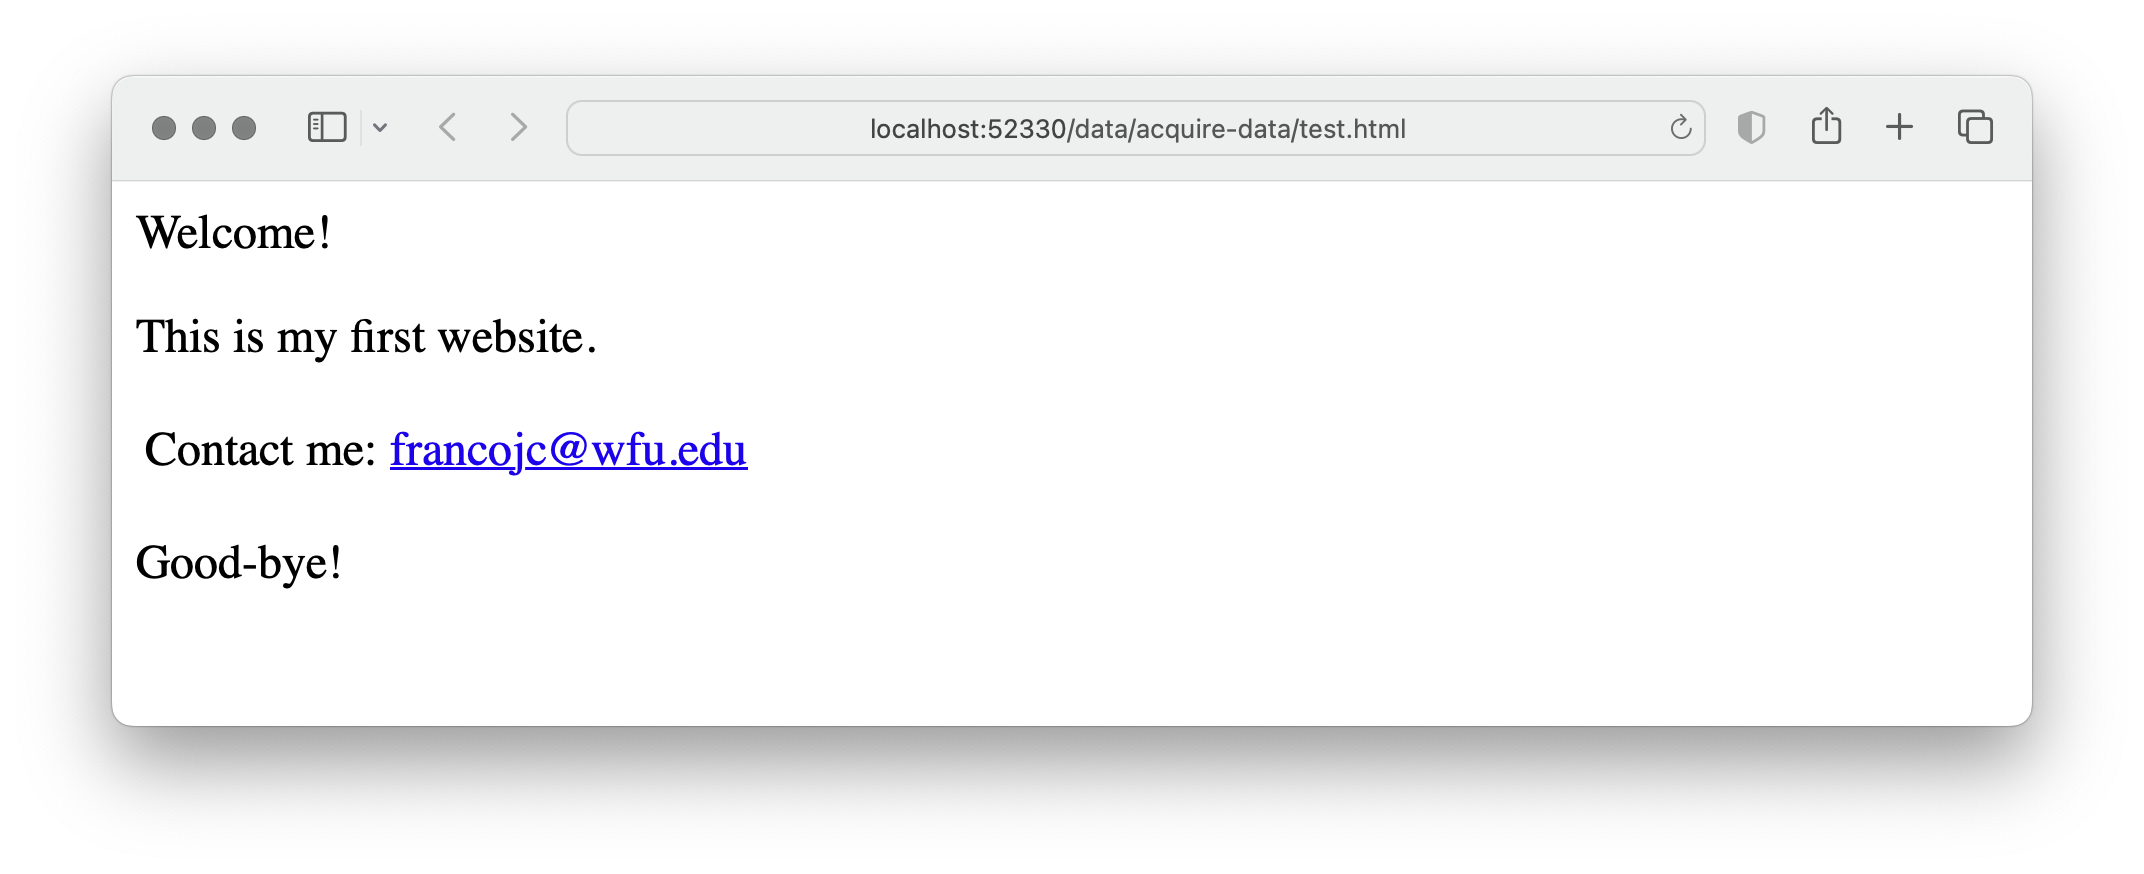
\includegraphics[width=1\textwidth,height=\textheight]{figures/acquire-data/ad-test-html.png}

}

\caption{\label{fig-ad-example-webpage}Example web page.}

\end{figure}

The file accessed by my browser to render this webpage is
\texttt{test.html} and in plain-text format as seen in
Example~\ref{exm-ad-html-structure}.

\begin{example}[]\protect\hypertarget{exm-ad-html-structure}{}\label{exm-ad-html-structure}

~

\begin{Shaded}
\begin{Highlighting}[]
\DataTypeTok{\textless{}!DOCTYPE }\NormalTok{html PUBLIC "{-}//W3C//DTD HTML 4.0 Transitional//EN" "http://www.w3.org/TR/REC{-}html40/loose.dtd"}\DataTypeTok{\textgreater{}}
\KeywordTok{\textless{}html\textgreater{}}
  \KeywordTok{\textless{}head\textgreater{}}
    \KeywordTok{\textless{}meta} \ErrorTok{http{-}equiv}\OtherTok{=}\StringTok{"Content{-}Type"} \ErrorTok{content}\OtherTok{=}\StringTok{"text/html; charset=UTF{-}8"} \KeywordTok{/\textgreater{}}
    \KeywordTok{\textless{}title\textgreater{}}\NormalTok{My website}\KeywordTok{\textless{}/title\textgreater{}}
  \KeywordTok{\textless{}/head\textgreater{}}
  \KeywordTok{\textless{}body\textgreater{}}
    \KeywordTok{\textless{}div} \ErrorTok{class}\OtherTok{=}\StringTok{"intro"}\KeywordTok{\textgreater{}}
      \KeywordTok{\textless{}p\textgreater{}}\NormalTok{Welcome!}\KeywordTok{\textless{}/p\textgreater{}}
      \KeywordTok{\textless{}p\textgreater{}}\NormalTok{This is my first website.}\KeywordTok{\textless{}/p\textgreater{}}
    \KeywordTok{\textless{}/div\textgreater{}}
    \KeywordTok{\textless{}table\textgreater{}}
      \KeywordTok{\textless{}tr\textgreater{}}
        \KeywordTok{\textless{}td\textgreater{}}\NormalTok{Contact me:}\KeywordTok{\textless{}/td\textgreater{}}
        \KeywordTok{\textless{}td\textgreater{}}
          \KeywordTok{\textless{}a} \ErrorTok{href}\OtherTok{=}\StringTok{"mailto:francojc@wfu.edu"}\KeywordTok{\textgreater{}}\NormalTok{francojc@wfu.edu}\KeywordTok{\textless{}/a\textgreater{}}
        \KeywordTok{\textless{}/td\textgreater{}}
      \KeywordTok{\textless{}/tr\textgreater{}}
    \KeywordTok{\textless{}/table\textgreater{}}
    \KeywordTok{\textless{}div} \ErrorTok{class}\OtherTok{=}\StringTok{"conc"}\KeywordTok{\textgreater{}}
      \KeywordTok{\textless{}p\textgreater{}}\NormalTok{Good{-}bye!}\KeywordTok{\textless{}/p\textgreater{}}
    \KeywordTok{\textless{}/div\textgreater{}}
  \KeywordTok{\textless{}/body\textgreater{}}
\KeywordTok{\textless{}/html\textgreater{}}
\end{Highlighting}
\end{Shaded}

\end{example}

Each element in this file is delineated by an opening and closing tag,
\texttt{\textless{}head\textgreater{}\textless{}/head\textgreater{}}.
Tags are nested within other tags to create the structural hierarchy.
Tags can take class and id labels to distinguish them from other tags
and often contain other attributes that dictate how the tag is to behave
when rendered visually by a browser. For example, there are two
\texttt{\textless{}div\textgreater{}} tags in our toy example: one has
the label \texttt{class\ =\ "intro"} and the other
\texttt{class\ =\ "conc"}. \texttt{\textless{}div\textgreater{}} tags
are often used to separate sections of a webpage that may require
special visual formatting. The \texttt{\textless{}a\textgreater{}} tag,
on the other hand, creates a web link. As part of this tag's function,
it requires the attribute \texttt{href=} and a web protocol --in this
case it is a link to an email address \texttt{mailto:francojc@wfu.edu}.
More often than not, however, the \texttt{href=} contains a URL (Uniform
Resource Locator). A working example might look like this:
\texttt{\textless{}a\ href="https://francojc.github.io/"\textgreater{}My\ homepage\textless{}/a\textgreater{}}.

The aim of a web scrape is to download the HTML file(s) that contain the
data we are interested in. This will include more information that we
may ultimately need, but by downloading the raw source HTML we are
effectively creating a local archive, or copy, of the webpage. Thus, if
the webpage is updated or removed from the web, we will still have
access to the data we accessed.

Later in the curation process we will parse (\emph{i.e.} read and
extract) target information that is relevant for the research at hand.
However, it often useful to parse the raw HTML in the process of
acquiring data if we are interested in harvesting data from multiple
pages and we would like to use the HTML structure to guide our data
extraction (\emph{i.e.} URLs to other pages)

To provide some preliminary background on working with HTML, we will use
the toy example above to demonstrate how to read and parse HTML using R.
To do this we will use the
\href{https://CRAN.R-project.org/package=rvest}{rvest}(\protect\hyperlink{ref-R-rvest}{Wickham
2022}) package. First, install/load the package, then, read and parse
the HTML from the character vector named \texttt{web\_file} assigning
the result to \texttt{html}.

\begin{example}[]\protect\hypertarget{exm-ad-read-html-toy}{}\label{exm-ad-read-html-toy}

~

\begin{Shaded}
\begin{Highlighting}[]
\CommentTok{\# Load package}
\FunctionTok{library}\NormalTok{(rvest) }\CommentTok{\# read and parse HTML}

\NormalTok{html }\OtherTok{\textless{}{-}} \FunctionTok{read\_html}\NormalTok{(web\_file) }\CommentTok{\# retrieve raw html}
\NormalTok{html}
\end{Highlighting}
\end{Shaded}

\begin{verbatim}
> {html_document}
> <html>
> [1] <head>\n<meta http-equiv="Content-Type" content="text/html; charset=UTF-8 ...
> [2] <body>\n    <div class="intro">\n      <p>Welcome!</p>\n      <p>This is  ...
\end{verbatim}

\end{example}

In Example~\ref{exm-ad-read-html-toy} \texttt{read\_html()} retrieves
the raw HTML and it makes it accessible to parsing in R. Being a subtype
of XML, \texttt{read\_html()} converts the raw HTML into an object of
class \texttt{xml\_document}, as we can see by calling \texttt{class()}
on the \texttt{html} object in
Example~\ref{exm-ad-class-html-toy-class}.

\begin{example}[]\protect\hypertarget{exm-ad-class-html-toy-class}{}\label{exm-ad-class-html-toy-class}

~

\begin{Shaded}
\begin{Highlighting}[]
\FunctionTok{class}\NormalTok{(html)}
\end{Highlighting}
\end{Shaded}

\begin{verbatim}
> [1] "xml_document" "xml_node"
\end{verbatim}

\end{example}

An object of class \texttt{xml\_document} represents each HTML tag as a
node. The tag nodes are elements can be accessed by using the
\texttt{html\_elements()} function by specifying the tag/node/element to
isolate.

\begin{example}[]\protect\hypertarget{exm-ad-parse-html-toy-1}{}\label{exm-ad-parse-html-toy-1}

~

\begin{Shaded}
\begin{Highlighting}[]
\NormalTok{html }\SpecialCharTok{|\textgreater{}}
  \FunctionTok{html\_elements}\NormalTok{(}\StringTok{"div"}\NormalTok{)}
\end{Highlighting}
\end{Shaded}

\begin{verbatim}
> {xml_nodeset (2)}
> [1] <div class="intro">\n      <p>Welcome!</p>\n      <p>This is my first web ...
> [2] <div class="conc">\n      <p>Good-bye!</p>\n    </div>
\end{verbatim}

\end{example}

Notice that the output of Example~\ref{exm-ad-parse-html-toy-1} has
returned both \texttt{div} tags and their respective children, tags
contained within. To isolate one of tags by its class, we add the class
name to the tag separating it with a \texttt{.}.

\begin{example}[]\protect\hypertarget{exm-ad-parse-html-toy-2}{}\label{exm-ad-parse-html-toy-2}

~

\begin{Shaded}
\begin{Highlighting}[]
\NormalTok{html }\SpecialCharTok{|\textgreater{}}
  \FunctionTok{html\_elements}\NormalTok{(}\StringTok{"div.intro"}\NormalTok{)}
\end{Highlighting}
\end{Shaded}

\begin{verbatim}
> {xml_nodeset (1)}
> [1] <div class="intro">\n      <p>Welcome!</p>\n      <p>This is my first web ...
\end{verbatim}

\end{example}

Great. Now say we want to drill down and isolate the subordinate
\texttt{\textless{}p\textgreater{}} nodes. We can add \texttt{p} to our
node filter, as in Example~\ref{exm-ad-parse-html-toy-3}.

\begin{example}[]\protect\hypertarget{exm-ad-parse-html-toy-3}{}\label{exm-ad-parse-html-toy-3}

~

\begin{Shaded}
\begin{Highlighting}[]
\NormalTok{html }\SpecialCharTok{|\textgreater{}}
  \FunctionTok{html\_elements}\NormalTok{(}\StringTok{"div.intro p"}\NormalTok{)}
\end{Highlighting}
\end{Shaded}

\begin{verbatim}
> {xml_nodeset (2)}
> [1] <p>Welcome!</p>
> [2] <p>This is my first website. </p>
\end{verbatim}

\end{example}

To extract the text contained within a node we use the
\texttt{html\_text()} function.

\begin{example}[]\protect\hypertarget{exm-ad-parse-html-toy-4}{}\label{exm-ad-parse-html-toy-4}

~

\begin{Shaded}
\begin{Highlighting}[]
\NormalTok{html }\SpecialCharTok{|\textgreater{}}
  \FunctionTok{html\_elements}\NormalTok{(}\StringTok{"div.intro p"}\NormalTok{) }\SpecialCharTok{|\textgreater{}}
  \FunctionTok{html\_text}\NormalTok{()}
\end{Highlighting}
\end{Shaded}

\begin{verbatim}
> [1] "Welcome!"                   "This is my first website. "
\end{verbatim}

\end{example}

The result of Example~\ref{exm-ad-parse-html-toy-4} is a character
vector with two elements corresponding to the text contained in each
\texttt{\textless{}p\textgreater{}} tag. If you were paying close
attention you might have noticed that the second element in our vector
includes extra whitespace after the period. To trim leading and trailing
whitespace from text we can add the \texttt{trim\ =\ TRUE} argument to
\texttt{html\_text()}, as in Example~\ref{exm-ad-parse-html-toy-5}.

\begin{example}[]\protect\hypertarget{exm-ad-parse-html-toy-5}{}\label{exm-ad-parse-html-toy-5}

~

\begin{Shaded}
\begin{Highlighting}[]
\NormalTok{html }\SpecialCharTok{|\textgreater{}}
  \FunctionTok{html\_elements}\NormalTok{(}\StringTok{"div.intro p"}\NormalTok{) }\SpecialCharTok{|\textgreater{}}
  \FunctionTok{html\_text}\NormalTok{(}\AttributeTok{trim =} \ConstantTok{TRUE}\NormalTok{)}
\end{Highlighting}
\end{Shaded}

\begin{verbatim}
> [1] "Welcome!"                  "This is my first website."
\end{verbatim}

\end{example}

With this basic understanding of how to read and parse HTML, we can now
turn to a more realistic example.

\hypertarget{federalist-papers}{%
\subsubsection{Federalist Papers}\label{federalist-papers}}

Say we investigate the authorship question of the the Federalist Papers
following in the footsteps of Mosteller and Wallace
(\protect\hyperlink{ref-Mosteller1963}{1963}). We want to scrape the
text of the Federalist Papers from the Library of Congress website. The
main page for the Federalist Papers is located at
\emph{https://guides.loc.gov/federalist-papers/full-text} and can be
seen in Figure~\ref{fig-ad-web-scrape-screenshot}.

\begin{figure}[H]

{\centering 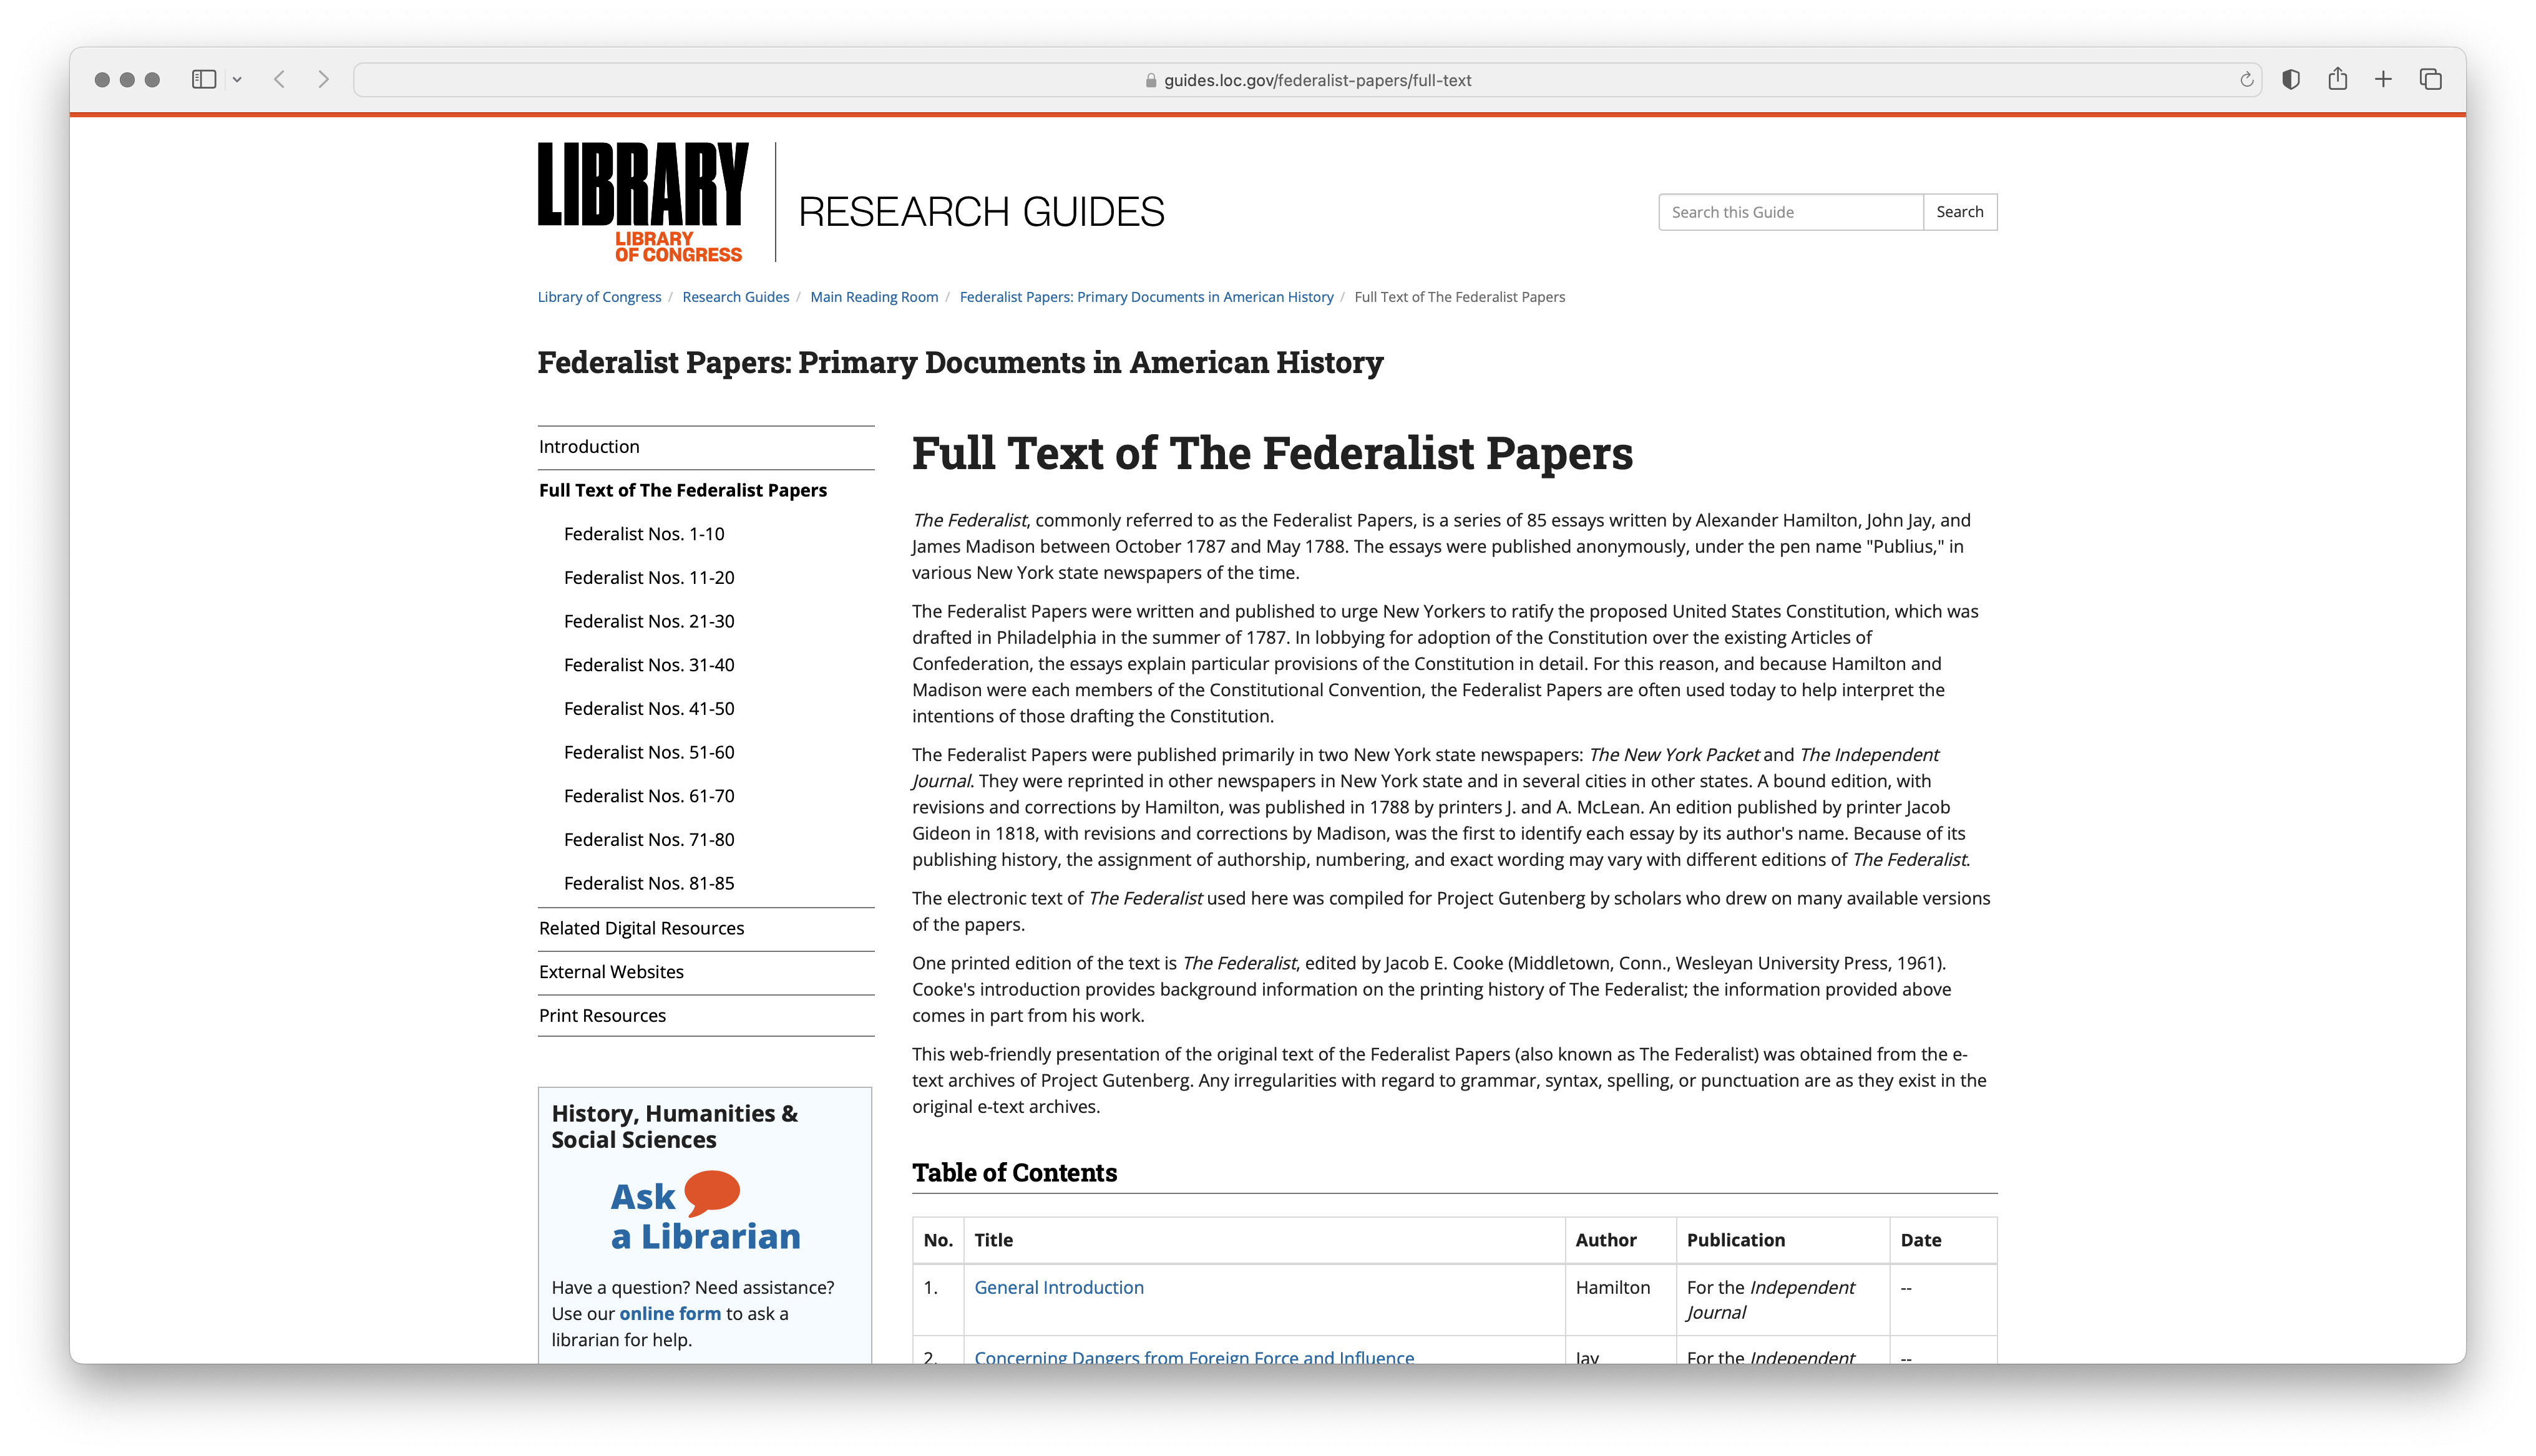
\includegraphics[width=1\textwidth,height=\textheight]{figures/acquire-data/ad-fed-papers-loc-main.png}

}

\caption{\label{fig-ad-web-scrape-screenshot}Screenshot of the Library
of Congress website for the Federalist Papers}

\end{figure}

The main page contains links to the text of each of the 85 papers. Our
goal will be to scrape and archive the raw HTML for this page and then
parse the HTML to extract the links to each of the papers. We will then
scrape and archive the raw HTML for each of the 85 papers.

The first step in any web scrape is to investigate the site and page(s)
we want to scrape to ascertain if there any licensing restrictions.
Many, but not all websites, will include a plain text file
\href{https://www.cloudflare.com/learning/bots/what-is-robots.txt/}{\texttt{robots.txt}}
at the root of the main URL. This file is declares which webpages a
`robot' (including web scraping scripts) can and cannot access. We can
use the \texttt{robotstxt} package to find out which URLs are accessible
\footnote{It is important to check the paths of sub-domains as some
  website allow access in some areas and not in others}.

\begin{example}[]\protect\hypertarget{exm-ad-fed-permissions}{}\label{exm-ad-fed-permissions}

~

\begin{Shaded}
\begin{Highlighting}[]
\CommentTok{\# Install and load package}
\NormalTok{pacman}\SpecialCharTok{::}\FunctionTok{p\_load}\NormalTok{(robotstxt)}

\CommentTok{\# URL for the Federalist Papers (LOC)}
\NormalTok{url }\OtherTok{\textless{}{-}} \StringTok{"https://guides.loc.gov/federalist{-}papers/full{-}text"}

\CommentTok{\# Check permissions}
\FunctionTok{paths\_allowed}\NormalTok{(url)}
\end{Highlighting}
\end{Shaded}

\begin{verbatim}
> [1] TRUE
\end{verbatim}

\end{example}

The next step is to read and parse the raw HTML. We can do this using
the \texttt{read\_html()} function.

\begin{example}[]\protect\hypertarget{exm-ad-fed-read-html}{}\label{exm-ad-fed-read-html}

~

\begin{Shaded}
\begin{Highlighting}[]
\CommentTok{\# Read raw html and parse to xml}
\NormalTok{html }\OtherTok{\textless{}{-}} \FunctionTok{read\_html}\NormalTok{(url)}

\CommentTok{\# Preview html}
\NormalTok{html}
\end{Highlighting}
\end{Shaded}

\end{example}

\begin{verbatim}
> {html_document}
> <html lang="en">
> [1] <head>\n<meta http-equiv="X-UA-Compatible" content="IE=Edge">\n<meta http ...
> [2] <body class="s-lg-guide-body">\r\n<a id="s-lg-public-skiplink" class="ale ...
\end{verbatim}

At this point we have captured the raw HTML assigning it to the object
named \texttt{html}. Let's archive the raw HTML to a file in our project
directory. We can do this using the \texttt{write\_html()} function from
the \texttt{xml2} package (\protect\hyperlink{ref-R-xml2}{Wickham,
Hester, and Ooms 2023}).

\begin{example}[]\protect\hypertarget{exm-ad-fed-write-html}{}\label{exm-ad-fed-write-html}

~

\begin{Shaded}
\begin{Highlighting}[]
\CommentTok{\# Create directory for HTML files}
\FunctionTok{dir\_create}\NormalTok{(}\StringTok{"../data/original/federalist\_papers/"}\NormalTok{)}

\CommentTok{\# Write raw html to file}
\FunctionTok{write\_html}\NormalTok{(html, }\StringTok{"../data/original/federalist\_papers/main.html"}\NormalTok{)}
\end{Highlighting}
\end{Shaded}

\end{example}

Our update project directory structure can be seen in
Example~\ref{exm-ad-fed-project-dir}.

\begin{example}[]\protect\hypertarget{exm-ad-fed-project-dir}{}\label{exm-ad-fed-project-dir}

~

\begin{Shaded}
\begin{Highlighting}[]
\ExtensionTok{data/}
\KeywordTok{|}\ExtensionTok{──}\NormalTok{ analysis/}
\ExtensionTok{├──}\NormalTok{ derived/}
\ExtensionTok{└──}\NormalTok{ original/}
    \ExtensionTok{└──}\NormalTok{ federalist\_papers/}
        \ExtensionTok{└──}\NormalTok{ main.html}
\end{Highlighting}
\end{Shaded}

\end{example}

Now, we also want to scrape the HTML that contains of the pages
corresponding to the 85 Federalist Papers. Perusing the main page we can
see that papers are organized into nine groups, \emph{e.g.} ``Federalist
Nos. 1-10''. So our aim will be to scrape the HTML for each of these
nine pages. We can do this using the \texttt{rvest} package, but we need
to identify the HTML elements that contain the URLs first in the main
webpage we have in \texttt{html}.

To do this it is helpful to use a browser to inspect specific elements
of the webpage, much as we did in the toy example in
Example~\ref{exm-ad-html-structure}. To view the raw and displayed HTML,
your browser will be equipped with a command that you can enable by
hovering your mouse over the element of the page you want to target and
using a right click to select ``Inspect'' (Chrome) or ``Inspect
Element'' (Safari, Brave). This will split your browser window vertical
or horizontally showing you the displayed and raw HTML underlying the
webpage.

We can see the HTML elements that contain the URLs in
Figure~\ref{fig-ad-fed-inspect}.

\begin{figure}[H]

{\centering 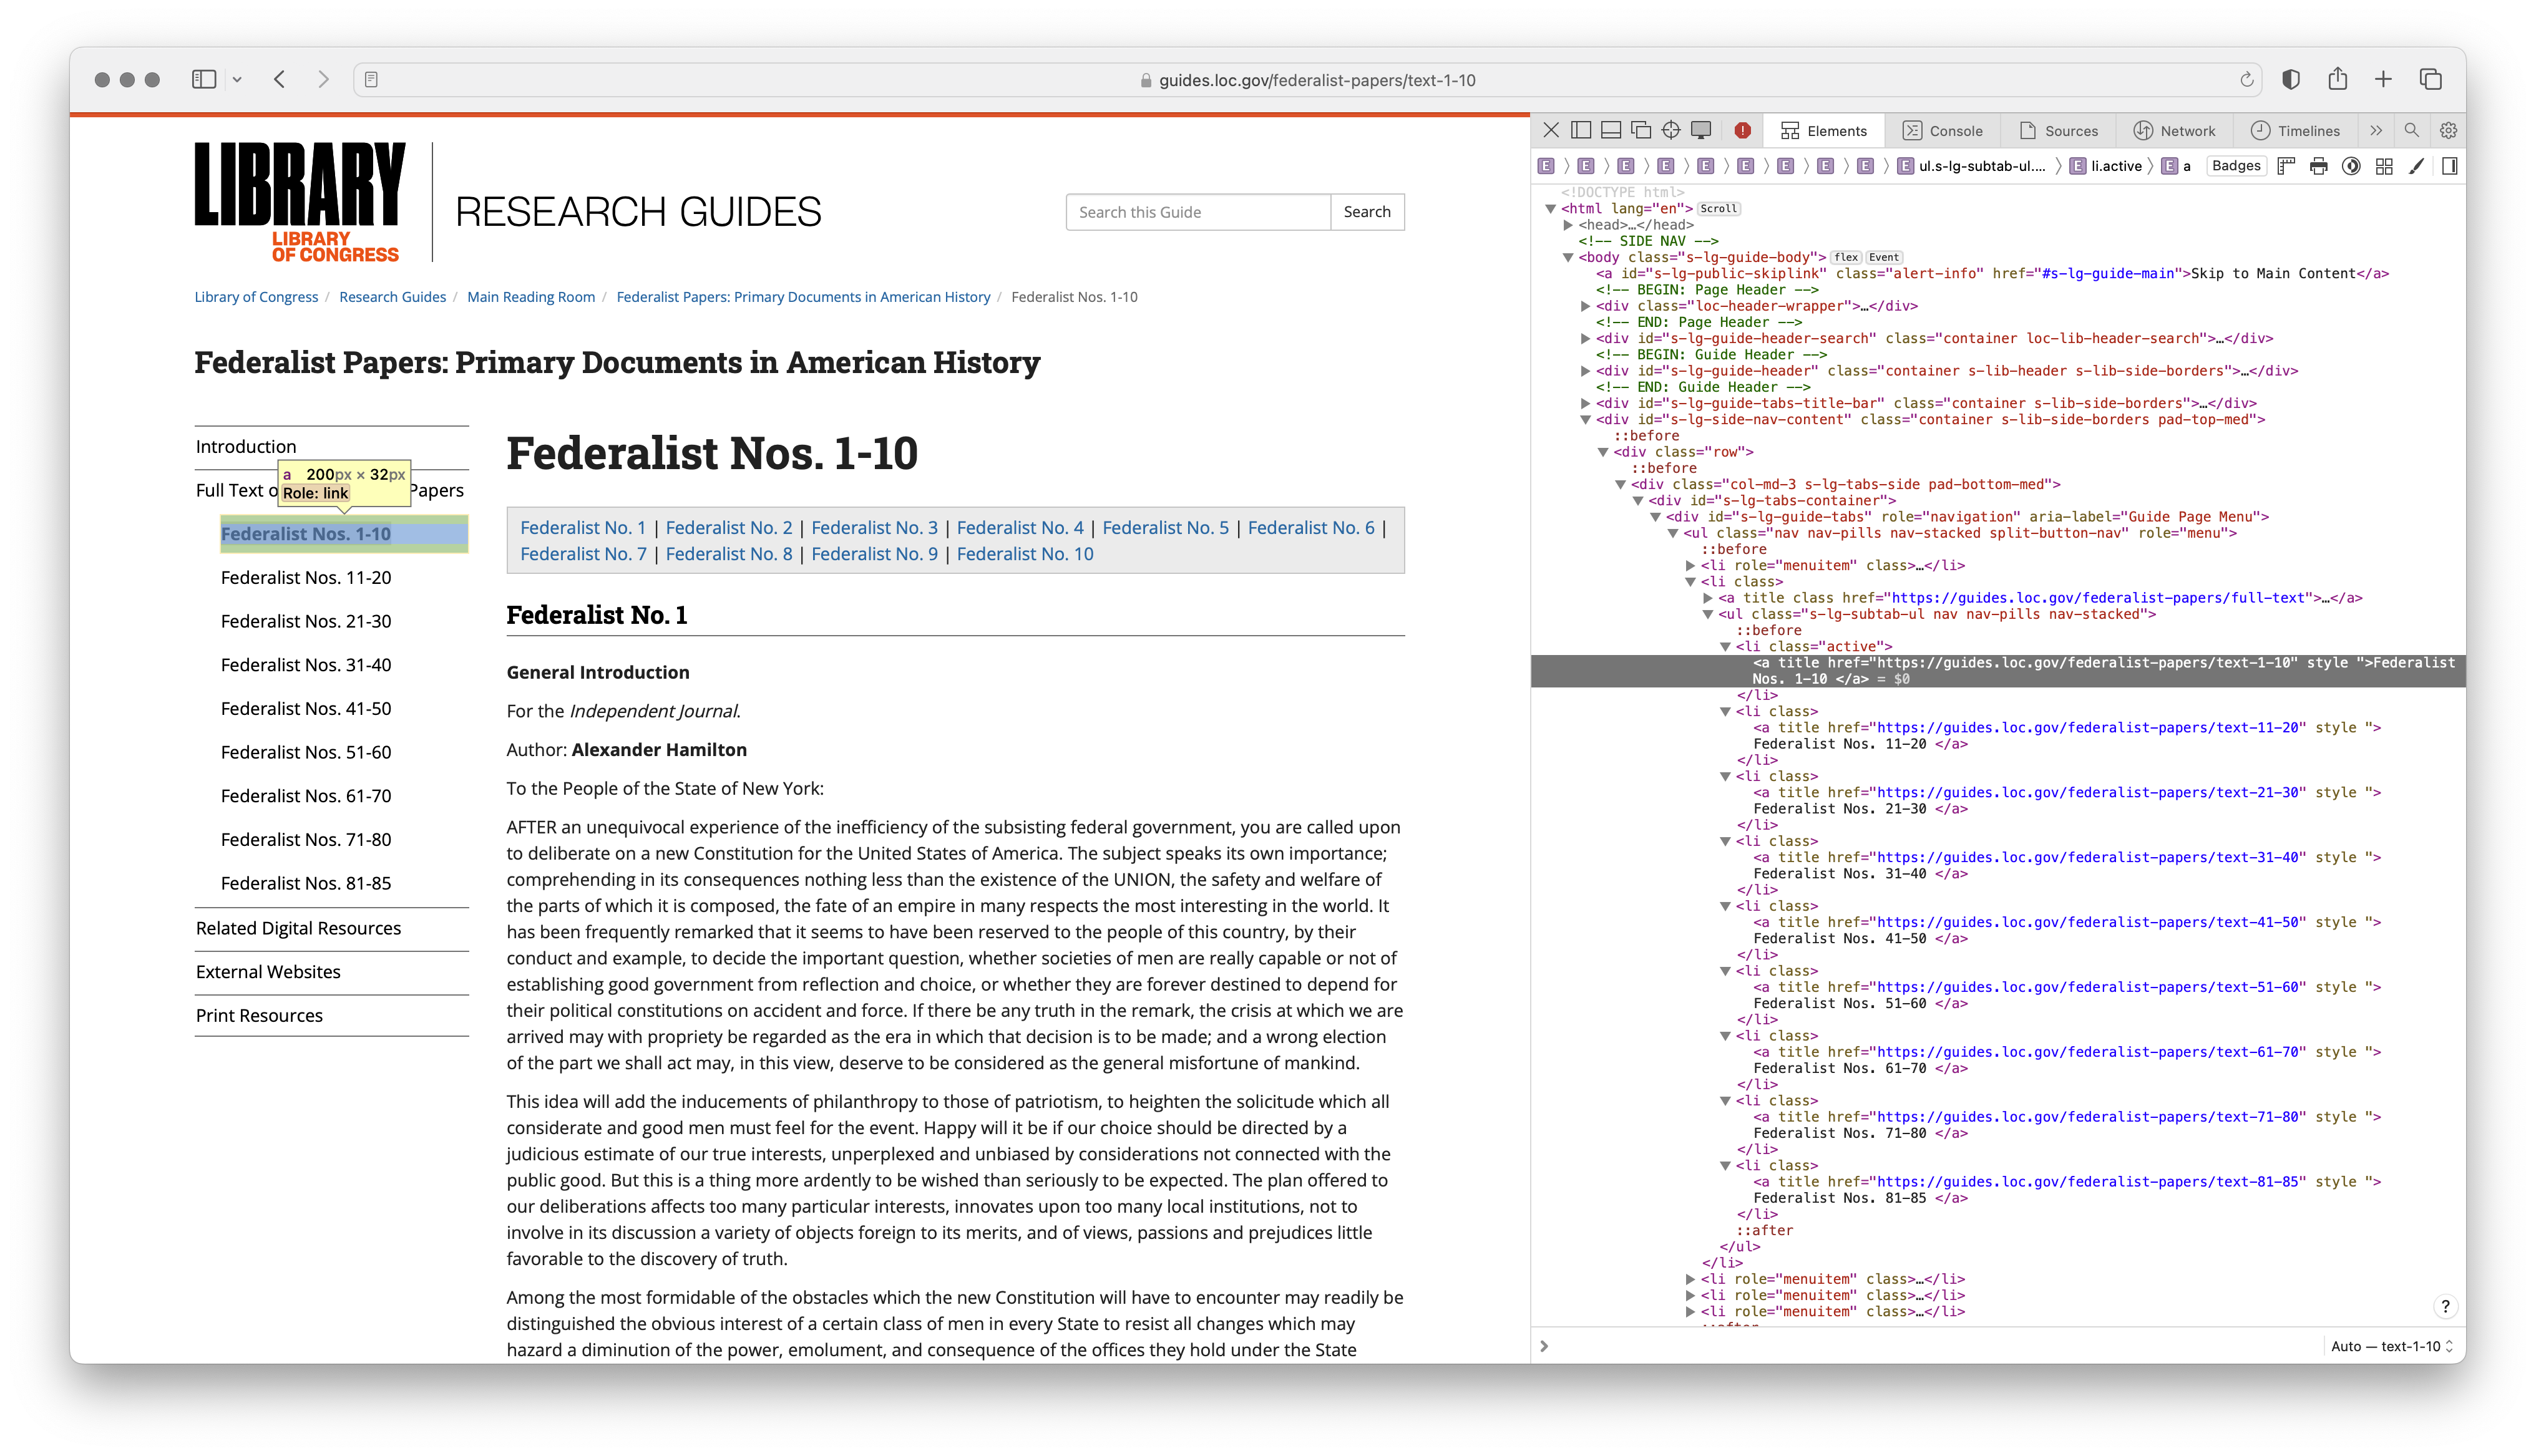
\includegraphics[width=1\textwidth,height=\textheight]{figures/acquire-data/ad-fed-papers-loc-inspect.png}

}

\caption{\label{fig-ad-fed-inspect}Screenshot of the HTML elements
containing the URLs for the Federalist Papers}

\end{figure}

Let's take a closer look at the source HTML in
Figure~\ref{fig-ad-fed-inspect-source} so we can inspect the elements
that contain the URLs and divise a strategy for isolating them to be
extracted.

\begin{figure}[H]

{\centering 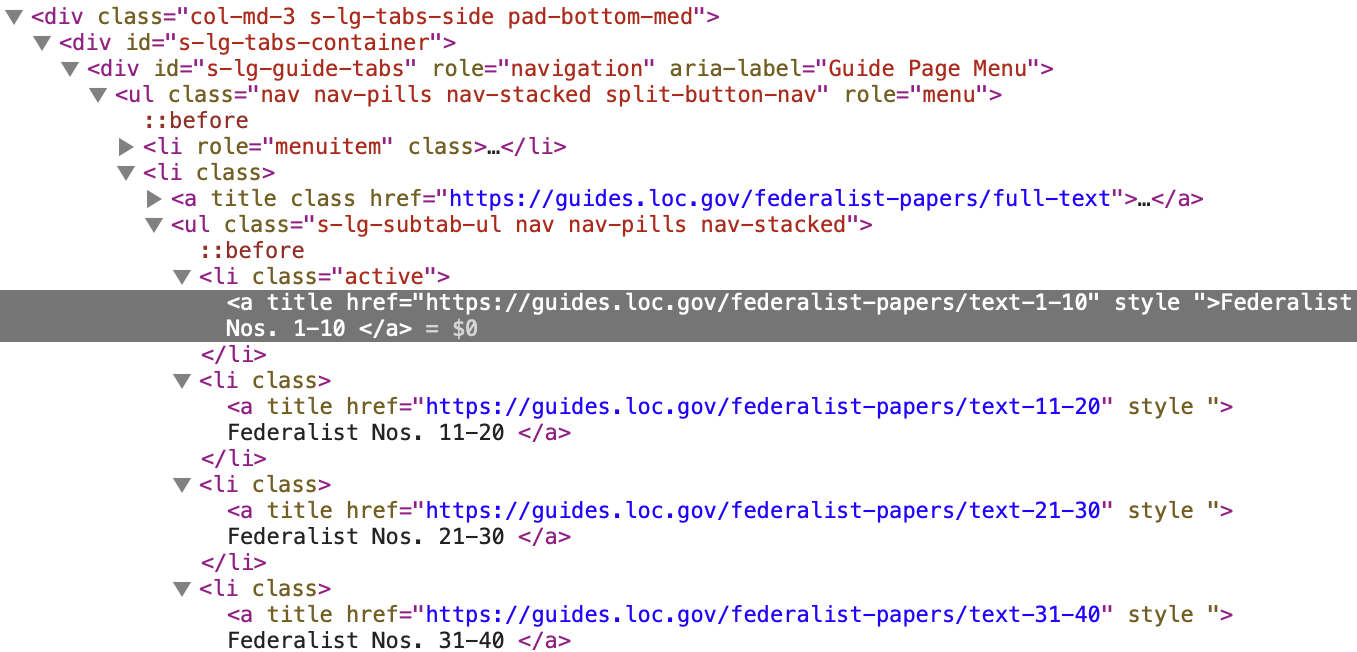
\includegraphics[width=1\textwidth,height=\textheight]{figures/acquire-data/ad-fed-papers-loc-inspect-source.png}

}

\caption{\label{fig-ad-fed-inspect-source}Screenshot of the source HTML
for the Federalist Papers}

\end{figure}

In Figure~\ref{fig-ad-fed-inspect-source} we can see that the HTML
elements that contain the URLs are nested within a
\texttt{\textless{}ul\textgreater{}} element. The
\texttt{\textless{}ul\textgreater{}} element has a set of class
attributes (\texttt{.s-lg-subtab-ul}, \texttt{nav}, \texttt{nav-pills},
\texttt{nav-stacked}). If one of these is unique to this
\texttt{\textless{}ul\textgreater{}} element we can use it to isolate
the element. Let's search the HTML for all the
\texttt{\textless{}ul\textgreater{}} elements on the page.

\begin{example}[]\protect\hypertarget{exm-ad-fed-papers-loc-url-ul}{}\label{exm-ad-fed-papers-loc-url-ul}

~

\begin{Shaded}
\begin{Highlighting}[]
\NormalTok{html }\SpecialCharTok{|\textgreater{}} 
  \FunctionTok{html\_nodes}\NormalTok{(}\StringTok{"ul"}\NormalTok{)}
\end{Highlighting}
\end{Shaded}

\begin{verbatim}
> {xml_nodeset (4)}
> [1] <ul class="nav nav-pills nav-stacked split-button-nav" role="menu">\n<li  ...
> [2] <ul class="s-lg-subtab-ul nav nav-pills nav-stacked">\n<li class=""><a ti ...
> [3] <ul id="s-lg-page-prevnext" class="pager s-lib-hide">\n<li class="previou ...
> [4] <ul id="s-lg-guide-header-attributes" class="">\n<li id="s-lg-guide-heade ...
\end{verbatim}

\end{example}

The output from Example~\ref{exm-ad-fed-papers-loc-url-ul} shows that
there are 4 \texttt{\textless{}ul\textgreater{}} elements on the page.
It's a little hard to see in the output, but the second
\texttt{\textless{}ul\textgreater{}} element is the one we are
targeting, as it contains the class attributes we identified in
Figure~\ref{fig-ad-fed-inspect-source}. We can use the
\texttt{html\_attr()} function to extract the \texttt{class} attribute
from the \texttt{\textless{}ul\textgreater{}} elements to see if one of
them is unique to the \texttt{\textless{}ul\textgreater{}} element we
want to isolate.

\begin{example}[]\protect\hypertarget{exm-ad-fed-papers-loc-url-ul-class}{}\label{exm-ad-fed-papers-loc-url-ul-class}

~

\begin{Shaded}
\begin{Highlighting}[]
\NormalTok{html }\SpecialCharTok{|\textgreater{}} 
  \FunctionTok{html\_nodes}\NormalTok{(}\StringTok{"ul"}\NormalTok{) }\SpecialCharTok{|\textgreater{}} 
  \FunctionTok{html\_attr}\NormalTok{(}\StringTok{"class"}\NormalTok{)}
\end{Highlighting}
\end{Shaded}

\begin{verbatim}
> [1] "nav nav-pills nav-stacked split-button-nav"
> [2] "s-lg-subtab-ul nav nav-pills nav-stacked"  
> [3] "pager s-lib-hide"                          
> [4] ""
\end{verbatim}

\end{example}

Effectively this is the case, as the second
\texttt{\textless{}ul\textgreater{}} element in the output of
Example~\ref{exm-ad-fed-papers-loc-url-ul-class} has a unique class
attribute, \texttt{.s-lg-subtab-ul}. We can use this to isolate the
element using the \texttt{html\_nodes()} function. We then pipe this to
another \texttt{html\_nodes()} function to isolate the
\texttt{\textless{}li\textgreater{}} elements nested within the
\texttt{\textless{}ul\textgreater{}} element. See
Example~\ref{exm-ad-fed-papers-loc-url-ul-class-s-lg-subtab-ul}.

\begin{example}[]\protect\hypertarget{exm-ad-fed-papers-loc-url-ul-class-s-lg-subtab-ul}{}\label{exm-ad-fed-papers-loc-url-ul-class-s-lg-subtab-ul}

~

\begin{Shaded}
\begin{Highlighting}[]
\NormalTok{html }\SpecialCharTok{|\textgreater{}} 
  \FunctionTok{html\_nodes}\NormalTok{(}\StringTok{"ul.s{-}lg{-}subtab{-}ul"}\NormalTok{) }\SpecialCharTok{|\textgreater{}} 
  \FunctionTok{html\_nodes}\NormalTok{(}\StringTok{"li"}\NormalTok{)}
\end{Highlighting}
\end{Shaded}

\begin{verbatim}
> {xml_nodeset (9)}
> [1] <li class=""><a title="" href="https://guides.loc.gov/federalist-papers/t ...
> [2] <li class=""><a title="" href="https://guides.loc.gov/federalist-papers/t ...
> [3] <li class=""><a title="" href="https://guides.loc.gov/federalist-papers/t ...
> [4] <li class=""><a title="" href="https://guides.loc.gov/federalist-papers/t ...
> [5] <li class=""><a title="" href="https://guides.loc.gov/federalist-papers/t ...
> [6] <li class=""><a title="" href="https://guides.loc.gov/federalist-papers/t ...
> [7] <li class=""><a title="" href="https://guides.loc.gov/federalist-papers/t ...
> [8] <li class=""><a title="" href="https://guides.loc.gov/federalist-papers/t ...
> [9] <li class=""><a title="" href="https://guides.loc.gov/federalist-papers/t ...
\end{verbatim}

\end{example}

Great. Now, to get the URLs we add another \texttt{html\_nodes()}
function to
Example~\ref{exm-ad-fed-papers-loc-url-ul-class-s-lg-subtab-ul} to
isolate the \texttt{\textless{}a\textgreater{}} elements nested within
the \texttt{\textless{}li\textgreater{}} elements and then a function
\texttt{html\_attr()} to extract the value of an attribute. In this
case, the attribute of the \texttt{\textless{}a\textgreater{}} elements
we want is \texttt{href}. See
Example~\ref{exm-ad-fed-papers-loc-url-ul-li-a}.

\begin{example}[]\protect\hypertarget{exm-ad-fed-papers-loc-url-ul-li-a}{}\label{exm-ad-fed-papers-loc-url-ul-li-a}

~

\begin{Shaded}
\begin{Highlighting}[]
\NormalTok{html }\SpecialCharTok{|\textgreater{}} 
  \FunctionTok{html\_nodes}\NormalTok{(}\StringTok{"ul.s{-}lg{-}subtab{-}ul"}\NormalTok{) }\SpecialCharTok{|\textgreater{}} 
  \FunctionTok{html\_nodes}\NormalTok{(}\StringTok{"li"}\NormalTok{) }\SpecialCharTok{|\textgreater{}} 
  \FunctionTok{html\_nodes}\NormalTok{(}\StringTok{"a"}\NormalTok{) }\SpecialCharTok{|\textgreater{}} 
  \FunctionTok{html\_attr}\NormalTok{(}\StringTok{"href"}\NormalTok{)}
\end{Highlighting}
\end{Shaded}

\begin{verbatim}
> [1] "https://guides.loc.gov/federalist-papers/text-1-10" 
> [2] "https://guides.loc.gov/federalist-papers/text-11-20"
> [3] "https://guides.loc.gov/federalist-papers/text-21-30"
> [4] "https://guides.loc.gov/federalist-papers/text-31-40"
> [5] "https://guides.loc.gov/federalist-papers/text-41-50"
> [6] "https://guides.loc.gov/federalist-papers/text-51-60"
> [7] "https://guides.loc.gov/federalist-papers/text-61-70"
> [8] "https://guides.loc.gov/federalist-papers/text-71-80"
> [9] "https://guides.loc.gov/federalist-papers/text-81-85"
\end{verbatim}

\end{example}

We can assign the URLs to a variable, \texttt{fed\_urls}.

With the URLs in hand, we can now retrieve the HTML for each of the nine
pages. We can, of course, do this manually, as in
Example~\ref{exm-ad-fed-papers-read-write-html-manual}.

\begin{example}[]\protect\hypertarget{exm-ad-fed-papers-read-write-html-manual}{}\label{exm-ad-fed-papers-read-write-html-manual}

~

\begin{Shaded}
\begin{Highlighting}[]
\CommentTok{\# Read the HTML from the first URL in \textasciigrave{}fed\_urls\textasciigrave{}}
\NormalTok{html }\OtherTok{\textless{}{-}} \FunctionTok{read\_html}\NormalTok{(fed\_urls[}\DecValTok{1}\NormalTok{])}
\FunctionTok{write\_html}\NormalTok{(html, }\StringTok{"../data/original/federalist\_papers/fed1.html"}\NormalTok{)}

\CommentTok{\# Read the HTML from the second URL in \textasciigrave{}fed\_urls\textasciigrave{}}
\NormalTok{html }\OtherTok{\textless{}{-}} \FunctionTok{read\_html}\NormalTok{(fed\_urls[}\DecValTok{2}\NormalTok{])}
\FunctionTok{write\_html}\NormalTok{(html, }\StringTok{"../data/original/federalist\_papers/fed2.html"}\NormalTok{)}

\CommentTok{\# ... and so on}
\end{Highlighting}
\end{Shaded}

\end{example}

But this is tedious and error prone, furthermore, it doesn't scale well.
If we had 1000 URLs to retrieve the HTML from, we would have to write
1000 lines of code. Instead, we can write a function to do this for us.
See Example~\ref{exm-ad-fed-papers-read-write-function}.

\begin{example}[]\protect\hypertarget{exm-ad-fed-papers-read-write-function}{}\label{exm-ad-fed-papers-read-write-function}

~

\begin{Shaded}
\begin{Highlighting}[]
\CommentTok{\# Function to retrieve HTML from a URL and write to a file}
\NormalTok{read\_write\_html }\OtherTok{\textless{}{-}} \ControlFlowTok{function}\NormalTok{(url) \{}
  \CommentTok{\# Create a file name and path from the URL}
\NormalTok{  file\_name }\OtherTok{\textless{}{-}} \FunctionTok{path\_file}\NormalTok{(url) }\SpecialCharTok{|\textgreater{}} \FunctionTok{path\_ext\_set}\NormalTok{(}\StringTok{".html"}\NormalTok{)}
\NormalTok{  file\_path }\OtherTok{\textless{}{-}} \FunctionTok{path}\NormalTok{(}\StringTok{"../data/original/federalist\_papers/"}\NormalTok{, file\_name)}

  \CommentTok{\# Read the HTML from the URL}
\NormalTok{  html }\OtherTok{\textless{}{-}} \FunctionTok{read\_html}\NormalTok{(url)}

  \CommentTok{\# Write the HTML to the file}
  \FunctionTok{write\_xml}\NormalTok{(html, file\_path)}
\NormalTok{\}}
\end{Highlighting}
\end{Shaded}

\end{example}

The function in Example~\ref{exm-ad-fed-papers-read-write-function}
takes a URL as it's only argument. It then creates a file name and path
from the URL. The file name is the last part of the URL, with the
extension \texttt{.html}. The file path is the path to the
\texttt{federalist\_papers} directory in the \texttt{data/original}
directory. The function then reads the HTML from the URL and writes it
to the file.

Example~\ref{exm-ad-fed-papers-read-write-function} might not seem like
a step up from Example~\ref{exm-ad-fed-papers-read-write-html-manual},
but it is. We can now use the \texttt{map()} function from
\texttt{purrr} to iterate over the URLs in \texttt{fed\_urls} and apply
the \texttt{read\_write\_html()} function to each URL. See
Example~\ref{exm-ad-fed-papers-read-write-map}.

\begin{example}[]\protect\hypertarget{exm-ad-fed-papers-read-write-map}{}\label{exm-ad-fed-papers-read-write-map}

~

\begin{Shaded}
\begin{Highlighting}[]
\CommentTok{\# Retrieve the HTML from each URL in \textasciigrave{}fed\_urls\textasciigrave{} and write to a file}
\NormalTok{fed\_urls }\SpecialCharTok{|\textgreater{}} 
  \FunctionTok{map}\NormalTok{(read\_write\_html)}
\end{Highlighting}
\end{Shaded}

\end{example}

\begin{tcolorbox}[enhanced jigsaw, rightrule=.15mm, leftrule=.75mm, opacityback=0, arc=.35mm, colback=white, breakable, toprule=.15mm, bottomrule=.15mm, left=2mm]

\textbf{\faIcon{hand-point-up} Tip}

When processing multiple webpages, it's often important to manage the
load on the server. In R, we can use the \texttt{Sys.sleep()} to
introduce short delays between requests. This helps reduce server load
when iterating over a list of webpages.

For example, we can use \texttt{Sys.sleep(1)} in our function to
introduce a 1 second delay between requests.

\begin{Shaded}
\begin{Highlighting}[]
\NormalTok{read\_write\_html }\OtherTok{\textless{}{-}} \ControlFlowTok{function}\NormalTok{(url) \{}
  \FunctionTok{Sys.sleep}\NormalTok{(}\DecValTok{1}\NormalTok{) }\CommentTok{\# 1 second delay}
  \CommentTok{\# ...}
\NormalTok{\}}
\end{Highlighting}
\end{Shaded}

Another tip is to use the \texttt{message()} function to print a status
message to the console. This can be helpful when processing a large
number of webpages.

\begin{Shaded}
\begin{Highlighting}[]
\NormalTok{read\_write\_html }\OtherTok{\textless{}{-}} \ControlFlowTok{function}\NormalTok{(url) \{}
  \FunctionTok{Sys.sleep}\NormalTok{(}\DecValTok{1}\NormalTok{) }\CommentTok{\# 1 second delay}
  \FunctionTok{message}\NormalTok{(}\StringTok{"Processing "}\NormalTok{, url) }\CommentTok{\# Prints: "Processing https://www.example.com"}
  \CommentTok{\# ...}
\NormalTok{\}}
\end{Highlighting}
\end{Shaded}

\end{tcolorbox}

The result of Example~\ref{exm-ad-fed-papers-read-write-map} can be seen
in the project directory in Example~\ref{exm-ad-fed-papers-directory}.

\begin{example}[]\protect\hypertarget{exm-ad-fed-papers-directory}{}\label{exm-ad-fed-papers-directory}

~

\begin{Shaded}
\begin{Highlighting}[]
\ExtensionTok{data/}
\KeywordTok{|}\ExtensionTok{{-}{-}}\NormalTok{ analysis/}
\KeywordTok{|}\ExtensionTok{{-}{-}}\NormalTok{ derived/}
\ExtensionTok{└──}\NormalTok{ original/}
    \ExtensionTok{└──}\NormalTok{ federalist\_papers/}
        \KeywordTok{|}\ExtensionTok{{-}{-}}\NormalTok{ main.html}
        \KeywordTok{|}\ExtensionTok{{-}{-}}\NormalTok{ text{-}1{-}10.html}
        \KeywordTok{|}\ExtensionTok{{-}{-}}\NormalTok{ text{-}11{-}20.html}
        \KeywordTok{|}\ExtensionTok{{-}{-}}\NormalTok{ text{-}21{-}30.html}
        \KeywordTok{|}\ExtensionTok{{-}{-}}\NormalTok{ text{-}31{-}40.html}
        \KeywordTok{|}\ExtensionTok{{-}{-}}\NormalTok{ text{-}41{-}50.html}
        \KeywordTok{|}\ExtensionTok{{-}{-}}\NormalTok{ text{-}51{-}60.html}
        \KeywordTok{|}\ExtensionTok{{-}{-}}\NormalTok{ text{-}61{-}70.html}
        \KeywordTok{|}\ExtensionTok{{-}{-}}\NormalTok{ text{-}71{-}80.html}
        \ExtensionTok{└──}\NormalTok{ text{-}81{-}85.html}
\end{Highlighting}
\end{Shaded}

\end{example}

And of course, to finish the acquisition process, we need to ensure we
have documented the code and created a data origin file. Since we have
created this resource it much of the information will be up to use to
document. Keep in mind that the data origin file should be written in a
way that is transparent to the researcher and to would-be collaborators
and the general research community.

In this section, we have built on previously introduced R coding
concepts and employed various others in the process of acquiring data
from the web. We have also considered topics that are more general in
nature and concern interacting with data found on the internet. As you
likely appreciate, web scraping often requires more knowledge of and
familiarity with R as well as other web technologies. Rest assured,
however, practice will increase confidence in your abilities. I
encourage you to practice on your own with other websites.

\hypertarget{summary-4}{%
\section*{Summary}\label{summary-4}}
\addcontentsline{toc}{section}{Summary}

\markright{Summary}

In this chapter we have covered a lot of ground. On the surface we have
discussed three methods for acquiring corpus data for use in text
analysis. In the process we have delved into various aspects of the R
programming language. Some key concepts include writing custom
functions, control statements, and applying functions iteratively. We
have also considered topics that are more general in nature and concern
interacting with data found on the internet.

Each of these methods should be approached in a way that is transparent
to the researcher and to would-be collaborators and the general research
community. For this reason the documentation of the steps taken to
acquire data are key both in the code and in human-facing documentation.

At this point you have both a bird's eye view of the data available on
the web and strategies on how to access a great majority of it. It is
now time to turn to the next step in our data analysis project: data
curation. In the next chapter, I will cover how to wrangle your raw data
into a tidy dataset.

\hypertarget{activities-3}{%
\section*{Activities}\label{activities-3}}
\addcontentsline{toc}{section}{Activities}

\markright{Activities}

\begin{itemize}
\tightlist
\item[$\square$]
  \faIcon{wrench} Add description of outcomes
\end{itemize}

\begin{tcolorbox}[enhanced jigsaw, rightrule=.15mm, leftrule=.75mm, opacityback=0, arc=.35mm, colback=white, breakable, toprule=.15mm, bottomrule=.15mm, left=2mm]

\textbf{\faIcon{file-code} Recipe}

\begin{itemize}
\tightlist
\item[$\square$]
  \faIcon{wrench} update
\end{itemize}

\textbf{What}:
\href{https://lin380.github.io/tadr/articles/recipe_6.html}{Control
statements, custom functions, and iteration}\\
\textbf{How}: Read Recipe 6 and participate in the Hypothes.is online
social annotation.\\
\textbf{Why}: To increase your ability to produce effective, concise,
and reproducible code. The three main areas we will cover are working
with control statements, writing custom functions, and leveraging
iteration. These programming strategies are often useful for acquiring
data but, as we will see, they are powerful concepts that can be used
throughout a reproducible research project.

\end{tcolorbox}

\begin{tcolorbox}[enhanced jigsaw, rightrule=.15mm, leftrule=.75mm, opacityback=0, arc=.35mm, colback=white, breakable, toprule=.15mm, bottomrule=.15mm, left=2mm]

\textbf{\faIcon{flask} Lab}

\begin{itemize}
\tightlist
\item[$\square$]
  \faIcon{wrench} update
\end{itemize}

\textbf{What}: \href{https://github.com/lin380/lab_6}{Control
statements, custom functions, and iteration}\\
\textbf{How}: Clone, fork, and complete the steps in Lab 6.\\
\textbf{Why}: To gain experience working with coding strategies such as
control statements, custom functions, and iteration, practice working
with direct downloads and API interfaces to acquire data, and implement
organizational strategies for organizing data in reproducible fashion.

\end{tcolorbox}

\hypertarget{questions-4}{%
\section*{Questions}\label{questions-4}}
\addcontentsline{toc}{section}{Questions}

\markright{Questions}

\begin{itemize}
\tightlist
\item[$\square$]
  \faIcon{wrench} create conceptual and technical questions
\end{itemize}

\begin{tcolorbox}[enhanced jigsaw, rightrule=.15mm, leftrule=.75mm, opacityback=0, arc=.35mm, colback=white, breakable, toprule=.15mm, bottomrule=.15mm, left=2mm]

\textbf{Conceptual questions}

\begin{itemize}
\tightlist
\item
  \ldots{}
\item
  For many resources, information to describe the data origin is found
  on the resource's website. Visit the XXX resource and complete the
  data origin information.
\end{itemize}

\end{tcolorbox}

\begin{tcolorbox}[enhanced jigsaw, rightrule=.15mm, leftrule=.75mm, opacityback=0, arc=.35mm, colback=white, breakable, toprule=.15mm, bottomrule=.15mm, left=2mm]

\textbf{Technical exercises}

\begin{itemize}
\tightlist
\item
  \ldots{}
\item
  \ldots{}
\end{itemize}

\end{tcolorbox}

\hypertarget{sec-curate-datasets}{%
\chapter{Curate datasets}\label{sec-curate-datasets}}

\begin{tcolorbox}[enhanced jigsaw, leftrule=.75mm, title=\textcolor{quarto-callout-caution-color}{\faFire}\hspace{0.5em}{Caution}, coltitle=black, opacityback=0, titlerule=0mm, arc=.35mm, bottomtitle=1mm, opacitybacktitle=0.6, colframe=quarto-callout-caution-color-frame, rightrule=.15mm, toptitle=1mm, left=2mm, colback=white, breakable, toprule=.15mm, bottomrule=.15mm, colbacktitle=quarto-callout-caution-color!10!white]

Under development.

\end{tcolorbox}

\hypertarget{sec-transform-datasets}{%
\chapter{Transform datasets}\label{sec-transform-datasets}}

\begin{tcolorbox}[enhanced jigsaw, leftrule=.75mm, title=\textcolor{quarto-callout-caution-color}{\faFire}\hspace{0.5em}{Caution}, coltitle=black, opacityback=0, titlerule=0mm, arc=.35mm, bottomtitle=1mm, opacitybacktitle=0.6, colframe=quarto-callout-caution-color-frame, rightrule=.15mm, toptitle=1mm, left=2mm, colback=white, breakable, toprule=.15mm, bottomrule=.15mm, colbacktitle=quarto-callout-caution-color!10!white]

Under development.

\end{tcolorbox}

\part{Analysis}

In this section we turn to the analysis of datasets, the evaluation of
results, and the interpretation of the findings. We will outline the
three main types of statistical analyses: Exploratory Data Analysis
(EDA), Predictive Data Analysis (PDA), and Inferential Data Analysis
(IDA). Each of these analysis types have distinct, non-overlapping aims
and therefore should be determined from the outset of the research
project and included as part of the research blueprint. The aim of this
section is to establish a clearer picture of the goals, methods, and
value of each of these approaches.

\hypertarget{sec-exploration}{%
\chapter{Exploration}\label{sec-exploration}}

\begin{tcolorbox}[enhanced jigsaw, leftrule=.75mm, title=\textcolor{quarto-callout-caution-color}{\faFire}\hspace{0.5em}{Caution}, coltitle=black, opacityback=0, titlerule=0mm, arc=.35mm, bottomtitle=1mm, opacitybacktitle=0.6, colframe=quarto-callout-caution-color-frame, rightrule=.15mm, toptitle=1mm, left=2mm, colback=white, breakable, toprule=.15mm, bottomrule=.15mm, colbacktitle=quarto-callout-caution-color!10!white]

Under development.

\end{tcolorbox}

\hypertarget{sec-prediction}{%
\chapter{Prediction}\label{sec-prediction}}

\begin{tcolorbox}[enhanced jigsaw, leftrule=.75mm, title=\textcolor{quarto-callout-caution-color}{\faFire}\hspace{0.5em}{Caution}, coltitle=black, opacityback=0, titlerule=0mm, arc=.35mm, bottomtitle=1mm, opacitybacktitle=0.6, colframe=quarto-callout-caution-color-frame, rightrule=.15mm, toptitle=1mm, left=2mm, colback=white, breakable, toprule=.15mm, bottomrule=.15mm, colbacktitle=quarto-callout-caution-color!10!white]

Under development.

\end{tcolorbox}

\hypertarget{sec-inference}{%
\chapter{Inference}\label{sec-inference}}

\begin{tcolorbox}[enhanced jigsaw, leftrule=.75mm, title=\textcolor{quarto-callout-caution-color}{\faFire}\hspace{0.5em}{Caution}, coltitle=black, opacityback=0, titlerule=0mm, arc=.35mm, bottomtitle=1mm, opacitybacktitle=0.6, colframe=quarto-callout-caution-color-frame, rightrule=.15mm, toptitle=1mm, left=2mm, colback=white, breakable, toprule=.15mm, bottomrule=.15mm, colbacktitle=quarto-callout-caution-color!10!white]

Under development.

\end{tcolorbox}

\part{Communication}

In this section I cover the steps in presenting the findings of the
research both as a research document and as a reproducible research
project. Both research documents and reproducible projects are
fundamental components of modern scientific inquiry. On the one hand a
research document provides readers a detailed summary of the main import
of the research study. On the other hand making the research project
available to interested readers ensures that the scientific community
can gain insight into the process implemented in the research and thus
enables researchers to vet and extend this research to build a more
robust and verifiable research base.

\hypertarget{sec-reports}{%
\chapter{Reports}\label{sec-reports}}

\begin{tcolorbox}[enhanced jigsaw, leftrule=.75mm, title=\textcolor{quarto-callout-caution-color}{\faFire}\hspace{0.5em}{Caution}, coltitle=black, opacityback=0, titlerule=0mm, arc=.35mm, bottomtitle=1mm, opacitybacktitle=0.6, colframe=quarto-callout-caution-color-frame, rightrule=.15mm, toptitle=1mm, left=2mm, colback=white, breakable, toprule=.15mm, bottomrule=.15mm, colbacktitle=quarto-callout-caution-color!10!white]

Under development.

\end{tcolorbox}

\hypertarget{sec-collaboration}{%
\chapter{Collaboration}\label{sec-collaboration}}

\begin{tcolorbox}[enhanced jigsaw, leftrule=.75mm, title=\textcolor{quarto-callout-caution-color}{\faFire}\hspace{0.5em}{Caution}, coltitle=black, opacityback=0, titlerule=0mm, arc=.35mm, bottomtitle=1mm, opacitybacktitle=0.6, colframe=quarto-callout-caution-color-frame, rightrule=.15mm, toptitle=1mm, left=2mm, colback=white, breakable, toprule=.15mm, bottomrule=.15mm, colbacktitle=quarto-callout-caution-color!10!white]

Under development.

\end{tcolorbox}

\bookmarksetup{startatroot}

\hypertarget{references}{%
\chapter*{References}\label{references}}
\addcontentsline{toc}{chapter}{References}

\markboth{References}{References}

\hypertarget{refs}{}
\begin{CSLReferences}{1}{0}
\leavevmode\vadjust pre{\hypertarget{ref-Ackoff1989}{}}%
Ackoff, Russell L. 1989. {``From Data to Wisdom.''} \emph{Journal of
Applied Systems Analysis} 16 (1): 3--9.

\leavevmode\vadjust pre{\hypertarget{ref-Adel2020}{}}%
Ädel, Annelie. 2020. {``Corpus Compilation.''} In \emph{A Practical
Handbook of Corpus Linguistics}, edited by Magali Paquot and Stefan Th.
Gries, 3--24. Switzerland: Springer.

\leavevmode\vadjust pre{\hypertarget{ref-Albert2015}{}}%
Albert, Saul, Laura E. de Ruiter, and J. P. de Ruiter. 2015. {``CABNC:
The Jeffersonian Transcription of the Spoken British National Corpus.''}
TalkBank.

\leavevmode\vadjust pre{\hypertarget{ref-R-quarto}{}}%
Allaire, JJ. 2022. \emph{Quarto: R Interface to Quarto Markdown
Publishing System}. \url{https://github.com/quarto-dev/quarto-r}.

\leavevmode\vadjust pre{\hypertarget{ref-R-rmarkdown}{}}%
Allaire, JJ, Yihui Xie, Christophe Dervieux, Jonathan McPherson, Javier
Luraschi, Kevin Ushey, Aron Atkins, et al. 2023. \emph{Rmarkdown:
Dynamic Documents for r}.
\url{https://CRAN.R-project.org/package=rmarkdown}.

\leavevmode\vadjust pre{\hypertarget{ref-Baayen2006}{}}%
Baayen, R. Harald, L. B. Feldman, and R. Schreuder. 2006.
{``Morphological Influences on the Recognition of Monosyllabic
Monomorphemic Words.''} \emph{Journal of Memory and Language} 55:
290--313. \url{https://doi.org/10.1016/j.jml.2006.03.008}.

\leavevmode\vadjust pre{\hypertarget{ref-Bao2019}{}}%
Bao, Wang, Ning Lianju, and Kong Yue. 2019. {``Integration of
Unsupervised and Supervised Machine Learning Algorithms for Credit Risk
Assessment.''} \emph{Expert Systems with Applications} 128 (August):
301--15. \url{https://doi.org/10.1016/j.eswa.2019.02.033}.

\leavevmode\vadjust pre{\hypertarget{ref-R-quanteda.corpora}{}}%
Benoit, Kenneth. 2020. \emph{Quanteda.corpora: A Collection of Corpora
for Quanteda}. \url{http://github.com/quanteda/quanteda.corpora}.

\leavevmode\vadjust pre{\hypertarget{ref-R-stopwords}{}}%
Benoit, Kenneth, David Muhr, and Kohei Watanabe. 2021. \emph{Stopwords:
Multilingual Stopword Lists}.
\url{https://github.com/quanteda/stopwords}.

\leavevmode\vadjust pre{\hypertarget{ref-R-workflowr}{}}%
Blischak, John, Peter Carbonetto, and Matthew Stephens. 2021.
\emph{Workflowr: A Framework for Reproducible and Collaborative Data
Science}. \url{https://github.com/workflowr/workflowr}.

\leavevmode\vadjust pre{\hypertarget{ref-R-wordbankr}{}}%
Braginsky, Mika. 2022. \emph{Wordbankr: Accessing the Wordbank
Database}. \url{https://CRAN.R-project.org/package=wordbankr}.

\leavevmode\vadjust pre{\hypertarget{ref-Bresnan2007a}{}}%
Bresnan, Joan. 2007. {``A Few Lessons from Typology.''} \emph{Linguistic
Typology} 11 (1): 297--306.

\leavevmode\vadjust pre{\hypertarget{ref-Brown2005}{}}%
Brown, Keith. 2005. \emph{Encyclopedia of Language and Linguistics}.
Vol. 1. Elsevier.

\leavevmode\vadjust pre{\hypertarget{ref-Buckheit1995}{}}%
Buckheit, Jonathan B., and David L. Donoho. 1995. {``Wavelab and
Reproducible Research.''} In \emph{Wavelets and Statistics}, 55--81.
Springer.

\leavevmode\vadjust pre{\hypertarget{ref-Bychkovska2017}{}}%
Bychkovska, Tetyana, and Joseph J. Lee. 2017. {``At the Same Time:
Lexical Bundles in L1 and L2 University Student Argumentative
Writing.''} \emph{Journal of English for Academic Purposes} 30
(November): 38--52. \url{https://doi.org/10.1016/j.jeap.2017.10.008}.

\leavevmode\vadjust pre{\hypertarget{ref-Campbell2001}{}}%
Campbell, Lyle. 2001. {``The History of Linguistics.''} In \emph{The
Handbook of Linguistics}, edited by Mark Aronoff and Janie Rees-Miller,
81--104. Blackwell Handbooks in Linguistics. Blackwell Publishers.

\leavevmode\vadjust pre{\hypertarget{ref-Carmi2020}{}}%
Carmi, Elinor, Simeon J. Yates, Eleanor Lockley, and Alicja Pawluczuk.
2020. {``Data Citizenship: Rethinking Data Literacy in the Age of
Disinformation, Misinformation, and Malinformation.''} \emph{Internet
Policy Review} 9 (2).

\leavevmode\vadjust pre{\hypertarget{ref-Chambers2020}{}}%
Chambers, John M. 2020. {``S, r, and Data Science.''} \emph{Proceedings
of the ACM on Programming Languages} 4 (HOPL): 1--17.
\url{https://doi.org/10.1145/3386334}.

\leavevmode\vadjust pre{\hypertarget{ref-Chan2014}{}}%
Chan, Sin-wai. 2014. \emph{Routledge Encyclopedia of Translation
Technology}. Routledge.

\leavevmode\vadjust pre{\hypertarget{ref-Conway2012}{}}%
Conway, Lucian Gideon, Laura Janelle Gornick, Chelsea Burfeind, Paul
Mandella, Andrea Kuenzli, Shannon C. Houck, and Deven Theresa Fullerton.
2012. {``Does Complex or Simple Rhetoric Win Elections? An Integrative
Complexity Analysis of u.s. Presidential Campaigns.''} \emph{Political
Psychology} 33 (5): 599--618.
\url{https://doi.org/10.1111/j.1467-9221.2012.00910.x}.

\leavevmode\vadjust pre{\hypertarget{ref-Cross2006}{}}%
Cross, Nigel. 2006. {``Design as a Discipline.''} \emph{Designerly Ways
of Knowing}, 95--103.

\leavevmode\vadjust pre{\hypertarget{ref-DataNeverSleeps08-2021}{}}%
{``Data Never Sleeps 7.0 Infographic.''} 2019.
https://www.domo.com/learn/infographic/data-never-sleeps-7.

\leavevmode\vadjust pre{\hypertarget{ref-Desjardins2019}{}}%
Desjardins, Jeff. 2019. {``How Much Data Is Generated Each Day?''}
\emph{Visual Capitalist}.

\leavevmode\vadjust pre{\hypertarget{ref-Donoho2017}{}}%
Donoho, David. 2017. {``50 Years of Data Science.''} \emph{Journal of
Computational and Graphical Statistics} 26 (4): 745--66.
\url{https://doi.org/10.1080/10618600.2017.1384734}.

\leavevmode\vadjust pre{\hypertarget{ref-Dubnjakovic2010}{}}%
Dubnjakovic, Ana, and Patrick Tomlin. 2010. \emph{A Practical Guide to
Electronic Resources in the Humanities}. Elsevier.

\leavevmode\vadjust pre{\hypertarget{ref-Eisenstein2012}{}}%
Eisenstein, Jacob, Brendan O'Connor, Noah A Smith, and Eric P Xing.
2012. {``Mapping the Geographical Diffusion of New Words.''}
\emph{Computation and Language}, 1--13.
\url{https://doi.org/10.1371/journal.pone.0113114}.

\leavevmode\vadjust pre{\hypertarget{ref-Francom2022}{}}%
Francom, Jerid. 2022. {``Corpus Studies of Syntax.''} In \emph{The
Cambridge Handbook of Experimental Syntax}, edited by Grant Goodall,
687--713. Cambridge Handbooks in Language and Linguistics. Cambridge
University Press.

\leavevmode\vadjust pre{\hypertarget{ref-R-qtalrkit}{}}%
---------. 2023. \emph{Qtalrkit: Quantitative Text Analysis for
Linguists Resource Kit}.

\leavevmode\vadjust pre{\hypertarget{ref-Gandrud2015}{}}%
Gandrud, Christopher. 2015.
\emph{\href{https://www.ncbi.nlm.nih.gov/pubmed/17811671}{Reproducible
Research with r and r Studio}}. Second edition. CRC Press.

\leavevmode\vadjust pre{\hypertarget{ref-Gentleman2007}{}}%
Gentleman, Robert, and Duncan Temple Lang. 2007. {``Statistical Analyses
and Reproducible Research.''} \emph{Journal of Computational and
Graphical Statistics} 16 (1): 1--23.

\leavevmode\vadjust pre{\hypertarget{ref-Gilquin2009}{}}%
Gilquin, Gaëtanelle, and Stefan Th Gries. 2009. {``Corpora and
Experimental Methods: A State-of-the-Art Review.''} \emph{Corpus
Linguistics and Linguistic Theory} 5 (1): 1--26.
\url{https://doi.org/10.1515/CLLT.2009.001}.

\leavevmode\vadjust pre{\hypertarget{ref-Gomez-Uribe2015}{}}%
Gomez-Uribe, Carlos A., and Neil Hunt. 2015. {``The Netflix Recommender
System: Algorithms, Business Value, and Innovation.''} \emph{ACM
Transactions on Management Information Systems (TMIS)} 6 (4): 1--19.

\leavevmode\vadjust pre{\hypertarget{ref-Gries2021a}{}}%
Gries, Stefan Th. 2021. \emph{Statistics for Linguistics with r}. De
Gruyter Mouton.

\leavevmode\vadjust pre{\hypertarget{ref-Gries2013a}{}}%
Gries, Stefan Th. 2013. \emph{Statistics for Linguistics with r. A
Practical Introduction}. 2nd revise.

\leavevmode\vadjust pre{\hypertarget{ref-Grieve2018}{}}%
Grieve, Jack, Andrea Nini, and Diansheng Guo. 2018. {``Mapping Lexical
Innovation on American Social Media.''} \emph{Journal of English
Linguistics} 46 (4): 293--319.

\leavevmode\vadjust pre{\hypertarget{ref-Hay2002}{}}%
Hay, Jennifer. 2002. {``From Speech Perception to Morphology: Affix
Ordering Revisited.''} \emph{Language} 78 (3): 527--55.

\leavevmode\vadjust pre{\hypertarget{ref-R-fs}{}}%
Hester, Jim, Hadley Wickham, and Gábor Csárdi. 2023. \emph{Fs:
Cross-Platform File System Operations Based on Libuv}.
\url{https://CRAN.R-project.org/package=fs}.

\leavevmode\vadjust pre{\hypertarget{ref-Hicks2019}{}}%
Hicks, Stephanie C., and Roger D. Peng. 2019. {``Elements and Principles
for Characterizing Variation Between Data Analyses.''} arXiv.
\url{https://doi.org/10.48550/arXiv.1903.07639}.

\leavevmode\vadjust pre{\hypertarget{ref-Ide2008}{}}%
Ide, Nancy, Collin Baker, Christiane Fellbaum, Charles Fillmore, and
Rebecca Passonneau. 2008. {``MASC: The Manually Annotated Sub-Corpus of
American English.''} In \emph{6th International Conference on Language
Resources and Evaluation, LREC 2008}, 2455--60. European Language
Resources Association (ELRA).

\leavevmode\vadjust pre{\hypertarget{ref-Ignatow2017}{}}%
Ignatow, Gabe, and Rada Mihalcea. 2017. \emph{An Introduction to Text
Mining: Research Design, Data Collection, and Analysis}. Sage
Publications.

\leavevmode\vadjust pre{\hypertarget{ref-Jaeger2007}{}}%
Jaeger, T Florian, and Neal Snider. 2007. {``Implicit Learning and
Syntactic Persistence: Surprisal and Cumulativity.''} \emph{University
of Rochester Working Papers in the Language Sciences} 3 (1).

\leavevmode\vadjust pre{\hypertarget{ref-Kaur2018}{}}%
Kaur, Jashanjot, and P. Kaur Buttar. 2018. {``A Systematic Review on
Stopword Removal Algorithms.''} \emph{International Journal on Future
Revolution in Computer Science \& Communication Engineering} 4 (4):
207--10.

\leavevmode\vadjust pre{\hypertarget{ref-Kloumann2012}{}}%
Kloumann, IM, CM Danforth, KD Harris, and CA Bliss. 2012. {``Positivity
of the English Language.''} \emph{PloS One}.

\leavevmode\vadjust pre{\hypertarget{ref-Kostic2003}{}}%
Kostić, Aleksandar, Tanja Marković, and Aleksandar Baucal. 2003.
{``Inflectional Morphology and Word Meaning: Orthogonal or
Co-Implicative Cognitive Domains?''} In \emph{Morphological Structure in
Language Processing}, edited by R. Harald Baayen and Robert Schreuder,
1--44. De Gruyter Mouton. \url{https://doi.org/10.1515/9783110910186.1}.

\leavevmode\vadjust pre{\hypertarget{ref-R-TBDBr}{}}%
Kowalski, John, and Rob Cavanaugh. 2022. \emph{TBDBr: Easy Access to
TalkBankDB via r API}.

\leavevmode\vadjust pre{\hypertarget{ref-Krathwohl2002}{}}%
Krathwohl, David R. 2002. {``A Revision of Bloom's Taxonomy: An
Overview.''} \emph{Theory into Practice} 41 (4): 212--18.

\leavevmode\vadjust pre{\hypertarget{ref-R-swirl}{}}%
Kross, Sean, Nick Carchedi, Bill Bauer, and Gina Grdina. 2020.
\emph{Swirl: Learn r, in r}. \url{http://swirlstats.com}.

\leavevmode\vadjust pre{\hypertarget{ref-Kucera1967}{}}%
Kucera, H, and W N Francis. 1967. \emph{Computational Analysis of
Present Day American English}. Brown University Press Providence.

\leavevmode\vadjust pre{\hypertarget{ref-R-targets}{}}%
Landau, William Michael. 2023. \emph{Targets: Dynamic Function-Oriented
Make-Like Declarative Pipelines}.
\url{https://CRAN.R-project.org/package=targets}.

\leavevmode\vadjust pre{\hypertarget{ref-Lantz2013}{}}%
Lantz, Brett. 2013. \emph{Machine Learning with r}. Birmingham: Packt
Publishing.

\leavevmode\vadjust pre{\hypertarget{ref-Leech1992}{}}%
Leech, Geoffrey. 1992. {``100 Million Words of English: The British
National Corpus (BNC),''} no. 1991: 1--13.

\leavevmode\vadjust pre{\hypertarget{ref-Lewis2004}{}}%
Lewis, Michael. 2004. \emph{Moneyball: The Art of Winning an Unfair
Game}. WW Norton \& Company.

\leavevmode\vadjust pre{\hypertarget{ref-Lozano2009}{}}%
Lozano, Cristóbal. 2009. {``CEDEL2: Corpus Escrito Del Español L2.''}
\emph{Applied Linguistics Now: Understanding Language and Mind/La
Lingüística Aplicada Hoy: Comprendiendo El Lenguaje y La Mente. Almería:
Universidad de Almería}, 197--212.

\leavevmode\vadjust pre{\hypertarget{ref-Magueresse2020}{}}%
Magueresse, Alexandre, Vincent Carles, and Evan Heetderks. 2020.
{``Low-Resource Languages: A Review of Past Work and Future
Challenges.''} arXiv. \url{https://arxiv.org/abs/2006.07264}.

\leavevmode\vadjust pre{\hypertarget{ref-Manning2003}{}}%
Manning, Christopher. 2003. {``Probabilistic Syntax.''} In
\emph{Probabilistic Linguistics}, edited by Bod, Jennifer Hay, and
Jannedy, 289--341. Cambridge, MA: MIT Press.

\leavevmode\vadjust pre{\hypertarget{ref-Marcus1993}{}}%
Marcus, Mitchell P, Beatrice Santorini, and Mary Ann Marcinkiewicz.
1993. {``Building a Large Annotated Corpus of English: The Penn
Treebank.''} \emph{Computational Linguistics} 19 (2): 313--30.

\leavevmode\vadjust pre{\hypertarget{ref-Marwick2018}{}}%
Marwick, Ben, Carl Boettiger, and Lincoln Mullen. 2018. {``Packaging
Data Analytical Work Reproducibly Using r (and Friends).''} \emph{The
American Statistician} 72 (1): 80--88.

\leavevmode\vadjust pre{\hypertarget{ref-R-lingtypology}{}}%
Moroz, George. 2023. \emph{Lingtypology: Linguistic Typology and
Mapping}. \url{https://CRAN.R-project.org/package=lingtypology}.

\leavevmode\vadjust pre{\hypertarget{ref-Mosteller1963}{}}%
Mosteller, Frederick, and David L Wallace. 1963. {``Inference in an
Authorship Problem.''} \emph{Journal of the American Statistical
Association} 58 (302): 275--309.
\url{https://www.jstor.org/stable/2283270}.

\leavevmode\vadjust pre{\hypertarget{ref-Munoz2006}{}}%
Muñoz, Carmen, ed. 2006. \emph{Age and the Rate of Foreign Language
Learning}. 1st ed. Vol. 19. Second Language Acquisition Series.
Clevedon: Multilingual Matters.

\leavevmode\vadjust pre{\hypertarget{ref-Nisioi2016}{}}%
Nisioi, Sergiu, Ella Rabinovich, Liviu P. Dinu, and Shuly Wintner.
23-28, 2016-05. {``A Corpus of Native, Non-Native and Translated
Texts.''} In \emph{Proceedings of the Tenth International Conference on
Language Resources and Evaluation (LREC 2016)}. Portoro{z̆}, Slovenia:
European Language Resources Association (ELRA).

\leavevmode\vadjust pre{\hypertarget{ref-Nivre2016}{}}%
Nivre, Joakim, Marie-Catherine de Marneffe, Filip Ginter, Yoav Goldberg,
Jan Hajič, Christopher D Manning, Ryan McDonald, et al. 2016.
{``Universal Dependencies V1: A Multilingual Treebank Collection.''}
\emph{Proceedings of the Tenth International Conference on Language
Resources and Evaluation (LREC'16)}, 1659--66.

\leavevmode\vadjust pre{\hypertarget{ref-Olohan2008}{}}%
Olohan, Maeve. 2008. {``Leave It Out! Using a Comparable Corpus to
Investigate Aspects of Explicitation in Translation.''} \emph{Cadernos
de Tradução}, 153--69.

\leavevmode\vadjust pre{\hypertarget{ref-Paquot2020a}{}}%
Paquot, Magali, and Stefan Th. Gries, eds. 2020. \emph{A Practical
Handbook of Corpus Linguistics}. Switzerland: Springer.

\leavevmode\vadjust pre{\hypertarget{ref-Riehemann2001}{}}%
Riehemann, Susanne Z. 2001. {``A Constructional Approach to Idioms and
Word Formation.''} PhD thesis, Stanford.

\leavevmode\vadjust pre{\hypertarget{ref-R-pacman}{}}%
Rinker, Tyler, and Dason Kurkiewicz. 2019. \emph{Pacman: Package
Management Tool}. \url{https://github.com/trinker/pacman}.

\leavevmode\vadjust pre{\hypertarget{ref-Roediger2000}{}}%
Roediger, H. L. L, and K. B. B McDermott. 2000. {``Distortions of
Memory.''} \emph{The Oxford Handbook of Memory}, 149--62.

\leavevmode\vadjust pre{\hypertarget{ref-Rowley2007}{}}%
Rowley, Jennifer. 2007. {``The Wisdom Hierarchy: Representations of the
DIKW Hierarchy.''} \emph{Journal of Information Science} 33 (2):
163--80. \url{https://doi.org/10.1177/0165551506070706}.

\leavevmode\vadjust pre{\hypertarget{ref-Saxena2020}{}}%
Saxena, Shweta, and Manasi Gyanchandani. 2020. {``Machine Learning
Methods for Computer-Aided Breast Cancer Diagnosis Using Histopathology:
A Narrative Review.''} \emph{Journal of Medical Imaging and Radiation
Sciences} 51 (1): 182--93.

\leavevmode\vadjust pre{\hypertarget{ref-Talarico2003}{}}%
Talarico, Jennifer M., and David C. Rubin. 2003. {``Confidence, Not
Consistency, Characterizes Flashbulb Memories.''} \emph{Psychological
Science} 14 (5): 455--61. \url{https://doi.org/10.1111/1467-9280.02453}.

\leavevmode\vadjust pre{\hypertarget{ref-Tottie2011}{}}%
Tottie, Gunnel. 2011. {``Uh and Um as Sociolinguistic Markers in British
English.''} \emph{International Journal of Corpus Linguistics} 16 (2):
173--97.

\leavevmode\vadjust pre{\hypertarget{ref-SWDA2008}{}}%
University of Colorado Boulder. 2008. {``Switchboard Dialog Act Corpus.
Web Download.''} Linguistic Data Consortium.

\leavevmode\vadjust pre{\hypertarget{ref-Voigt2017}{}}%
Voigt, Rob, Nicholas P. Camp, Vinodkumar Prabhakaran, William L.
Hamilton, Rebecca C. Hetey, Camilla M. Griffiths, David Jurgens, Dan
Jurafsky, and Jennifer L. Eberhardt. 2017. {``Language from Police Body
Camera Footage Shows Racial Disparities in Officer Respect.''}
\emph{Proceedings of the National Academy of Sciences} 114 (25):
6521--26.

\leavevmode\vadjust pre{\hypertarget{ref-R-ProjectTemplate}{}}%
White, John Myles. 2023. \emph{ProjectTemplate: Automates the Creation
of New Statistical Analysis Projects}. \url{http://projecttemplate.net}.

\leavevmode\vadjust pre{\hypertarget{ref-Wickham2014a}{}}%
Wickham, Hadley. 2014. {``Tidy Data.''} \emph{Journal of Statistical
Software} 59 (10). \url{https://doi.org/10.18637/jss.v059.i10}.

\leavevmode\vadjust pre{\hypertarget{ref-R-rvest}{}}%
---------. 2022. \emph{Rvest: Easily Harvest (Scrape) Web Pages}.
\url{https://CRAN.R-project.org/package=rvest}.

\leavevmode\vadjust pre{\hypertarget{ref-R-tidyverse}{}}%
---------. 2023. \emph{Tidyverse: Easily Install and Load the
Tidyverse}. \url{https://CRAN.R-project.org/package=tidyverse}.

\leavevmode\vadjust pre{\hypertarget{ref-R-usethis}{}}%
Wickham, Hadley, Jennifer Bryan, Malcolm Barrett, and Andy Teucher.
2023. \emph{Usethis: Automate Package and Project Setup}.
\url{https://CRAN.R-project.org/package=usethis}.

\leavevmode\vadjust pre{\hypertarget{ref-R-dplyr}{}}%
Wickham, Hadley, Romain François, Lionel Henry, Kirill Müller, and Davis
Vaughan. 2023. \emph{Dplyr: A Grammar of Data Manipulation}.
\url{https://CRAN.R-project.org/package=dplyr}.

\leavevmode\vadjust pre{\hypertarget{ref-R-readr}{}}%
Wickham, Hadley, Jim Hester, and Jennifer Bryan. 2023. \emph{Readr: Read
Rectangular Text Data}. \url{https://CRAN.R-project.org/package=readr}.

\leavevmode\vadjust pre{\hypertarget{ref-R-devtools}{}}%
Wickham, Hadley, Jim Hester, Winston Chang, and Jennifer Bryan. 2022.
\emph{Devtools: Tools to Make Developing r Packages Easier}.
\url{https://CRAN.R-project.org/package=devtools}.

\leavevmode\vadjust pre{\hypertarget{ref-R-xml2}{}}%
Wickham, Hadley, Jim Hester, and Jeroen Ooms. 2023. \emph{Xml2: Parse
XML}. \url{https://CRAN.R-project.org/package=xml2}.

\leavevmode\vadjust pre{\hypertarget{ref-R-tidyr}{}}%
Wickham, Hadley, Davis Vaughan, and Maximilian Girlich. 2023.
\emph{Tidyr: Tidy Messy Data}.
\url{https://CRAN.R-project.org/package=tidyr}.

\leavevmode\vadjust pre{\hypertarget{ref-Wulff2007}{}}%
Wulff, S, A Stefanowitsch, and Stefan Th. Gries. 2007. {``Brutal Brits
and Persuasive Americans.''} \emph{Aspects of Meaning}.

\leavevmode\vadjust pre{\hypertarget{ref-R-bookdown}{}}%
Xie, Yihui. 2023a. \emph{Bookdown: Authoring Books and Technical
Documents with r Markdown}.
\url{https://CRAN.R-project.org/package=bookdown}.

\leavevmode\vadjust pre{\hypertarget{ref-R-tinytex}{}}%
---------. 2023b. \emph{Tinytex: Helper Functions to Install and
Maintain TeX Live, and Compile LaTeX Documents}.
\url{https://github.com/rstudio/tinytex}.

\end{CSLReferences}

\cleardoublepage
\phantomsection
\addcontentsline{toc}{part}{Appendices}
\appendix

\hypertarget{data-appendix}{%
\chapter{Data}\label{data-appendix}}

\ldots{}

\hypertarget{feedback-appendix}{%
\chapter{\texorpdfstring{Feedback
\faIcon{comment}}{Feedback }}\label{feedback-appendix}}

Thank you for taking the time to read through this book 🫶🏻. I really
value your opinion and I would love to hear your thoughts as I continue
to make progress.

\hypertarget{where-to-review}{%
\subsection*{Where to review}\label{where-to-review}}
\addcontentsline{toc}{subsection}{Where to review}

Chapters that are ready for feedback will appear with the following
callout.

\begin{tcolorbox}[enhanced jigsaw, leftrule=.75mm, title=\textcolor{quarto-callout-tip-color}{\faLightbulb}\hspace{0.5em}{Draft}, coltitle=black, opacityback=0, titlerule=0mm, arc=.35mm, bottomtitle=1mm, opacitybacktitle=0.6, colframe=quarto-callout-tip-color-frame, rightrule=.15mm, toptitle=1mm, left=2mm, colback=white, breakable, toprule=.15mm, bottomrule=.15mm, colbacktitle=quarto-callout-tip-color!10!white]

Ready for review.

\end{tcolorbox}

Those that are not ready will appear with the following callout.

\begin{tcolorbox}[enhanced jigsaw, leftrule=.75mm, title=\textcolor{quarto-callout-caution-color}{\faFire}\hspace{0.5em}{Caution}, coltitle=black, opacityback=0, titlerule=0mm, arc=.35mm, bottomtitle=1mm, opacitybacktitle=0.6, colframe=quarto-callout-caution-color-frame, rightrule=.15mm, toptitle=1mm, left=2mm, colback=white, breakable, toprule=.15mm, bottomrule=.15mm, colbacktitle=quarto-callout-caution-color!10!white]

Under development.

\end{tcolorbox}

In a few cases a chapter will be ready for review, but I'll still be
working on the exercises, callouts, \emph{etc.} In those cases, the
items that are still under development will be marked with the
\faIcon{wrench} icon.

\hypertarget{what-to-look-for}{%
\subsection*{What to look for}\label{what-to-look-for}}
\addcontentsline{toc}{subsection}{What to look for}

As you read over the draft, I'd appreciate your feedback in the
following areas:

\begin{enumerate}
\def\labelenumi{\arabic{enumi}.}
\item
  Clarity and Comprehensibility\\
  I'd love to know if you think the content is clear and easy to
  understand. Do you think the concepts are broken down enough? Are the
  examples helpful? If anything seems too jargon-y or confusing,
  definitely let me know.
\item
  Consistency\\
  It's pretty important to keep things smooth. So, keep an eye out for
  any inconsistent writing styles, terminology, or layout. If something
  seems off, I'd appreciate it if you point it out.
\item
  Relevance\\
  Does the material match the current standards and knowledge? Will it
  the topics and questions be of interest to linguists? If something
  feels outdated or irrelevant, don't hesitate to mention it.
\item
  Engagement\\
  \hspace{0pt}I\hspace{0pt}'m not looking to drop a boring read on
  people. So, as you're going through it, think about whether it holds
  your interest. Maybe \hspace{0pt}the prose needs more life, the
  examples need to be more diverse, or the exercises could be more or
  less challenging. If you have any ideas, I'm all ears.
\end{enumerate}

\hypertarget{how-to-submit-feedback}{%
\subsection*{How to submit feedback}\label{how-to-submit-feedback}}
\addcontentsline{toc}{subsection}{How to submit feedback}

Depending on your preference, you can submit feedback in one of three
ways:

\begin{itemize}
\item
  \href{https://hypothes.is/groups/wppaYKxy/qtal-feedback}{hypothes.is}\\
  This is the easiest way to submit feedback. Join the
  ``qtal\_feedback'' annotation group and just highlight the text you
  want to comment on and click the ``Annotate'' button. You can also add
  comments to the right sidebar.
\item
  \href{https://github.com/qtalr/book/issues}{GitHub issues}\\
  This book is hosted on GitHub, so you can submit feedback directly
  through the issues page for the repository. Just click the ``New
  issue'' button and fill out the form. You'll need a GitHub account to
  do this.
\item
  Email me at
  \href{mailto:francojc@wfu.edu}{\nolinkurl{francojc@wfu.edu}}\\
  If you'd rather not use the other options, you can always email me
  directly. Just make sure to try to include references to the specific
  parts of the book you're referring to. A link or section number will
  do.
\end{itemize}

\hypertarget{thank-yous}{%
\subsection*{Thank yous!}\label{thank-yous}}
\addcontentsline{toc}{subsection}{Thank yous!}

I want to thank you beforehand for your willingness to help me out. I
really appreciate it. I also want to thank you in print. Please give me
the name you would like to appear in the
\protect\hyperlink{acknowledgements}{Acknowledgements} section. If you'd
rather not be acknowledged in the final version of the book, please let
me know.



\printindex

\end{document}
